\documentclass[]{article}
\usepackage{lmodern}
\usepackage{amssymb,amsmath}
\usepackage{ifxetex,ifluatex}
\usepackage{fixltx2e} % provides \textsubscript
\ifnum 0\ifxetex 1\fi\ifluatex 1\fi=0 % if pdftex
  \usepackage[T1]{fontenc}
  \usepackage[utf8]{inputenc}
\else % if luatex or xelatex
  \ifxetex
    \usepackage{mathspec}
  \else
    \usepackage{fontspec}
  \fi
  \defaultfontfeatures{Ligatures=TeX,Scale=MatchLowercase}
\fi
% use upquote if available, for straight quotes in verbatim environments
\IfFileExists{upquote.sty}{\usepackage{upquote}}{}
% use microtype if available
\IfFileExists{microtype.sty}{%
\usepackage{microtype}
\UseMicrotypeSet[protrusion]{basicmath} % disable protrusion for tt fonts
}{}
\usepackage[margin=1in]{geometry}
\usepackage{hyperref}
\hypersetup{unicode=true,
            pdftitle={MAthesis},
            pdfborder={0 0 0},
            breaklinks=true}
\urlstyle{same}  % don't use monospace font for urls
\usepackage{color}
\usepackage{fancyvrb}
\newcommand{\VerbBar}{|}
\newcommand{\VERB}{\Verb[commandchars=\\\{\}]}
\DefineVerbatimEnvironment{Highlighting}{Verbatim}{commandchars=\\\{\}}
% Add ',fontsize=\small' for more characters per line
\usepackage{framed}
\definecolor{shadecolor}{RGB}{248,248,248}
\newenvironment{Shaded}{\begin{snugshade}}{\end{snugshade}}
\newcommand{\KeywordTok}[1]{\textcolor[rgb]{0.13,0.29,0.53}{\textbf{{#1}}}}
\newcommand{\DataTypeTok}[1]{\textcolor[rgb]{0.13,0.29,0.53}{{#1}}}
\newcommand{\DecValTok}[1]{\textcolor[rgb]{0.00,0.00,0.81}{{#1}}}
\newcommand{\BaseNTok}[1]{\textcolor[rgb]{0.00,0.00,0.81}{{#1}}}
\newcommand{\FloatTok}[1]{\textcolor[rgb]{0.00,0.00,0.81}{{#1}}}
\newcommand{\ConstantTok}[1]{\textcolor[rgb]{0.00,0.00,0.00}{{#1}}}
\newcommand{\CharTok}[1]{\textcolor[rgb]{0.31,0.60,0.02}{{#1}}}
\newcommand{\SpecialCharTok}[1]{\textcolor[rgb]{0.00,0.00,0.00}{{#1}}}
\newcommand{\StringTok}[1]{\textcolor[rgb]{0.31,0.60,0.02}{{#1}}}
\newcommand{\VerbatimStringTok}[1]{\textcolor[rgb]{0.31,0.60,0.02}{{#1}}}
\newcommand{\SpecialStringTok}[1]{\textcolor[rgb]{0.31,0.60,0.02}{{#1}}}
\newcommand{\ImportTok}[1]{{#1}}
\newcommand{\CommentTok}[1]{\textcolor[rgb]{0.56,0.35,0.01}{\textit{{#1}}}}
\newcommand{\DocumentationTok}[1]{\textcolor[rgb]{0.56,0.35,0.01}{\textbf{\textit{{#1}}}}}
\newcommand{\AnnotationTok}[1]{\textcolor[rgb]{0.56,0.35,0.01}{\textbf{\textit{{#1}}}}}
\newcommand{\CommentVarTok}[1]{\textcolor[rgb]{0.56,0.35,0.01}{\textbf{\textit{{#1}}}}}
\newcommand{\OtherTok}[1]{\textcolor[rgb]{0.56,0.35,0.01}{{#1}}}
\newcommand{\FunctionTok}[1]{\textcolor[rgb]{0.00,0.00,0.00}{{#1}}}
\newcommand{\VariableTok}[1]{\textcolor[rgb]{0.00,0.00,0.00}{{#1}}}
\newcommand{\ControlFlowTok}[1]{\textcolor[rgb]{0.13,0.29,0.53}{\textbf{{#1}}}}
\newcommand{\OperatorTok}[1]{\textcolor[rgb]{0.81,0.36,0.00}{\textbf{{#1}}}}
\newcommand{\BuiltInTok}[1]{{#1}}
\newcommand{\ExtensionTok}[1]{{#1}}
\newcommand{\PreprocessorTok}[1]{\textcolor[rgb]{0.56,0.35,0.01}{\textit{{#1}}}}
\newcommand{\AttributeTok}[1]{\textcolor[rgb]{0.77,0.63,0.00}{{#1}}}
\newcommand{\RegionMarkerTok}[1]{{#1}}
\newcommand{\InformationTok}[1]{\textcolor[rgb]{0.56,0.35,0.01}{\textbf{\textit{{#1}}}}}
\newcommand{\WarningTok}[1]{\textcolor[rgb]{0.56,0.35,0.01}{\textbf{\textit{{#1}}}}}
\newcommand{\AlertTok}[1]{\textcolor[rgb]{0.94,0.16,0.16}{{#1}}}
\newcommand{\ErrorTok}[1]{\textcolor[rgb]{0.64,0.00,0.00}{\textbf{{#1}}}}
\newcommand{\NormalTok}[1]{{#1}}
\usepackage{longtable,booktabs}
\usepackage{graphicx,grffile}
\makeatletter
\def\maxwidth{\ifdim\Gin@nat@width>\linewidth\linewidth\else\Gin@nat@width\fi}
\def\maxheight{\ifdim\Gin@nat@height>\textheight\textheight\else\Gin@nat@height\fi}
\makeatother
% Scale images if necessary, so that they will not overflow the page
% margins by default, and it is still possible to overwrite the defaults
% using explicit options in \includegraphics[width, height, ...]{}
\setkeys{Gin}{width=\maxwidth,height=\maxheight,keepaspectratio}
\IfFileExists{parskip.sty}{%
\usepackage{parskip}
}{% else
\setlength{\parindent}{0pt}
\setlength{\parskip}{6pt plus 2pt minus 1pt}
}
\setlength{\emergencystretch}{3em}  % prevent overfull lines
\providecommand{\tightlist}{%
  \setlength{\itemsep}{0pt}\setlength{\parskip}{0pt}}
\setcounter{secnumdepth}{0}
% Redefines (sub)paragraphs to behave more like sections
\ifx\paragraph\undefined\else
\let\oldparagraph\paragraph
\renewcommand{\paragraph}[1]{\oldparagraph{#1}\mbox{}}
\fi
\ifx\subparagraph\undefined\else
\let\oldsubparagraph\subparagraph
\renewcommand{\subparagraph}[1]{\oldsubparagraph{#1}\mbox{}}
\fi

%%% Use protect on footnotes to avoid problems with footnotes in titles
\let\rmarkdownfootnote\footnote%
\def\footnote{\protect\rmarkdownfootnote}

%%% Change title format to be more compact
\usepackage{titling}

% Create subtitle command for use in maketitle
\newcommand{\subtitle}[1]{
  \posttitle{
    \begin{center}\large#1\end{center}
    }
}

\setlength{\droptitle}{-2em}
  \title{MAthesis}
  \pretitle{\vspace{\droptitle}\centering\huge}
  \posttitle{\par}
  \author{}
  \preauthor{}\postauthor{}
  \date{}
  \predate{}\postdate{}

\usepackage{setspace}
\doublespacing

\begin{document}
\maketitle

{
\setcounter{tocdepth}{2}
\tableofcontents
}
\section{Time bins (stratigraphic
stages)}\label{time-bins-stratigraphic-stages}

\begin{longtable}[]{@{}lllrrrr@{}}
\caption{Smaller time bins with age range, epoch name, mean age and
corresponding sample sizes (on individual, species and genus
level)}\tabularnewline
\toprule
bin & EpochBins & Stages & MeanBins & nIndividuals & nSpecies &
nGenera\tabularnewline
\midrule
\endfirsthead
\toprule
bin & EpochBins & Stages & MeanBins & nIndividuals & nSpecies &
nGenera\tabularnewline
\midrule
\endhead
(0,0.0117{]} & Modern & Modern & 0.00585 & 253 & 65 & 18\tabularnewline
(0.0117,0.126{]} & Upper Pleistocene & Upper Pleistocene & 0.06885 & 49
& 18 & 8\tabularnewline
(0.126,0.781{]} & Middle Pleistocene & Middle Pleistocene & 0.45350 & 53
& 13 & 7\tabularnewline
(0.781,1.81{]} & Lower Pleistocene & Lower Pleistocene & 1.29350 & 57 &
27 & 12\tabularnewline
(1.81,2.59{]} & Gelasian & Lower Pleistocene & 2.19700 & 31 & 14 &
8\tabularnewline
(2.59,3.6{]} & Piacencian & Upper Pliocene & 3.09400 & 21 & 14 &
9\tabularnewline
(3.6,5.33{]} & Zanclean & Lower Pliocene & 4.46600 & 26 & 14 &
8\tabularnewline
(5.33,7.25{]} & Messinian & Upper Miocene & 6.28900 & 10 & 7 &
4\tabularnewline
(7.25,11.6{]} & Tortonian & Upper Miocene & 9.42700 & 45 & 20 &
9\tabularnewline
(11.6,13.8{]} & Serravallian & Middle Miocene & 12.71400 & 27 & 8 &
6\tabularnewline
(13.8,16{]} & Langhian & Middle Miocene & 14.89500 & 14 & 10 &
7\tabularnewline
(16,23{]} & Burdigalian/Aquitanian & Lower Miocene & 19.50000 & 30 & 14
& 9\tabularnewline
\bottomrule
\end{longtable}

\begin{figure}[htbp]
\centering
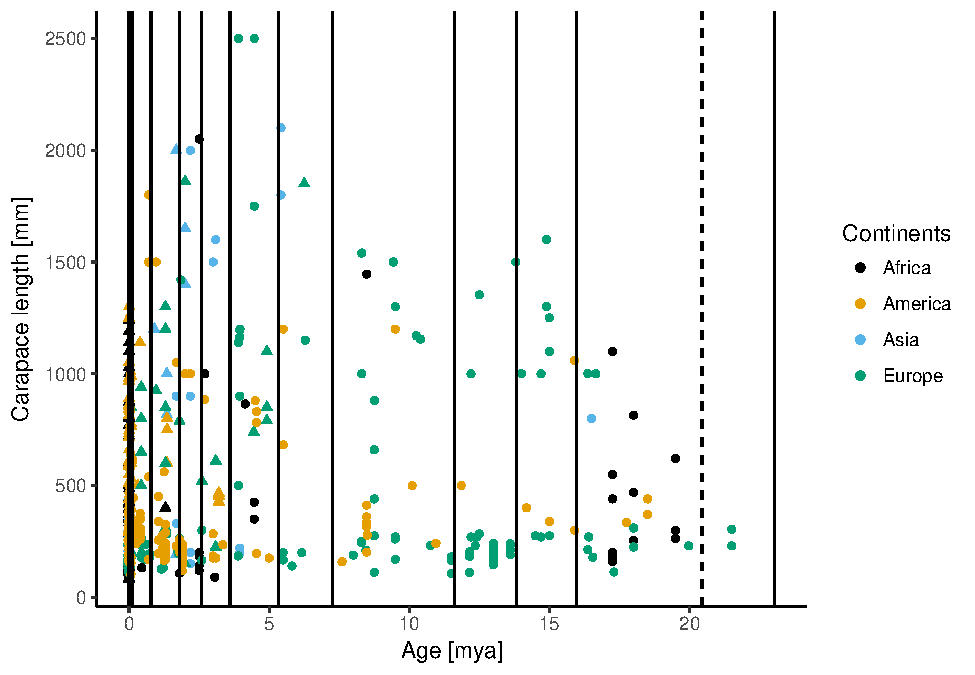
\includegraphics{MA_JJ_files/figure-latex/overviewData-1.pdf}
\caption{Scatterplot of carapace length over time, indicating insular
(triangle) and continental (circles) and colour indicating continents.
Lines indicate stratigraphic stages which were used as time bins, the
dashed line is the border between the two stages of the Lower Miocene,
which were consideres as one time bin.}
\end{figure}

\newpage

\section{Maps}\label{maps}

\subsection{fossil occurences of
testudinidae}\label{fossil-occurences-of-testudinidae}

\begin{verbatim}
## [1] 193
\end{verbatim}

\begin{longtable}[]{@{}lllrrrlll@{}}
\caption{fossil occurrences}\tabularnewline
\toprule
& Locality & Country & Latitude & Longitude & Age & Genus & Taxon &
Author\tabularnewline
\midrule
\endfirsthead
\toprule
& Locality & Country & Latitude & Longitude & Age & Genus & Taxon &
Author\tabularnewline
\midrule
\endhead
1 & Kabyle 2 km N, Yambol Region & Bulgaria & 42.54720 & 26.48430 &
0.0020 & Testudo & Testudo sp. & Linnaeus, 1758\tabularnewline
2 & El Harhoura 2 (Temara) & Morocco & 33.95220 & -6.92590 & 0.0050 &
Testudo & Testudo graeca & Linnaeus, 1758\tabularnewline
3 & El Harhoura 2 (Temara) & Morocco & 33.95220 & -6.92590 & 0.0050 &
Testudo & Testudo sp. & Linnaeus, 1758\tabularnewline
4 & Guenfouda Cave (Ghar Zebouj, ??????), Jerada Province & Morocco &
34.43300 & -2.00000 & 0.0060 & Testudo & Testudo sp. & Linnaeus,
1758\tabularnewline
5 & Brown Sand Wedge Local Fauna, Roosevelt County, New Mexico & USA &
34.00000 & -103.50000 & 0.0060 & Hesperotestudo & Hesperotestudo wilsoni
& (Milstead, 1956)\tabularnewline
6 & Blackwater Loc. No. 1, Roosevelt County, New Mexico & USA & 34.00000
& -103.50000 & 0.0110 & Hesperotstudo & Hesperotestudo cf.~wilsoni &
(Milstead, 1956)\tabularnewline
7 & Robledo Cave, west side of the Robledo Mountains, Doña Ana County,
New Mexico & USA & 33.00000 & -106.50000 & 0.0110 & Gopherus & Gopherus
agassizi & (Cooper, 1861)\tabularnewline
8 & Domebo Local Fauna, Caddo County, Oklahoma & USA & 36.00000 &
-100.00000 & 0.0110 & Hesperotestudo & Hesperotestudo wilsoni &
(Milstead, 1956)\tabularnewline
9 & Salt Creek, 4.7 mi S and 5.7 mi. W Orla, Reeves County, Texas & USA
& 31.78000 & -103.99000 & 0.0130 & Gopherus & Gopherus cf.~sp. &
Rafinesque, 1832\tabularnewline
10 & Schulze Cave Fauna, Edwards County, Texas & USA & 30.30000 &
-99.90000 & 0.0150 & Hesperotestudo & Hesperotestudo cf.~wilsoni &
(Milstead, 1956)\tabularnewline
11 & U-Bar Cave Late Wiskonsin, Hidalgo County, New Mexico & USA &
31.60000 & -108.40000 & 0.0175 & Geochelone & Geochelone cf.~sp. &
Rafinesque, 1832\tabularnewline
12 & Friesenhahn Cave, Bexar County, Texas & USA & 29.00000 & -98.00000
& 0.0180 & Hesperotestudo & Hesperotestudo wilsoni & (Milstead,
1956)\tabularnewline
13 & Gorham's cave IIIb, Gibraltar Peninsula & England & 36.12030 &
-5.34190 & 0.0200 & Eurotestudo & Eurotestudo hermanni & (Gmelin,
1789)\tabularnewline
14 & Gruta do Caldeirão, Tomar & Portugal & 39.60070 & -8.41380 & 0.0200
& Testudo & Testudo sp. & Linnaeus, 1758\tabularnewline
15 & Gruta do Escoural, Évora & Portugal & 38.57000 & -7.91000 & 0.0200
& Eurotestudo & Eurotestudo cf.~hermanni & (Gmelin, 1789)\tabularnewline
16 & Sims Bayou Local Fauna, Harris County, Texas & USA & 29.00000 &
-95.00000 & 0.0200 & Hesperotestudo & Hesperotestudo sp. & Williams,
1950\tabularnewline
17 & Shelter Cave (LACM 1010, UTEP 30), Doña Ana County, New Mexico &
USA & 33.00000 & -106.50000 & 0.0215 & Gopherus & Gopherus agassizi &
(Cooper, 1861)\tabularnewline
18 & Rancho La Brea, California & USA & 34.05220 & -118.24300 & 0.0240 &
Gopherus & Gopherus ? sp. & Rafinesque, 1832\tabularnewline
19 & Sabertooth Camel Maze, Dry Cave (UTEP 5), Eddy County, New Mexico &
USA & 32.00000 & -104.00000 & 0.0255 & Gopherus & Gopherus agassizi &
(Cooper, 1861)\tabularnewline
20 & Sabertooth Camel Maze, Dry Cave (UTEP 5), Eddy County, New Mexico &
USA & 32.00000 & -104.00000 & 0.0255 & Hesperotestudo & Hesperotestudo
wilsoni & (Milstead, 1956)\tabularnewline
21 & Gruta Nova da Columbeira, Bombarral & Portugal & 39.30510 &
-9.19530 & 0.0275 & Eurotestudo & Eurotestudo hermanni & (Gmelin,
1789)\tabularnewline
22 & Clear Creek Local Fauna, Denton County, Texas & USA & 33.20000 &
-97.10000 & 0.0280 & Hesperotestudo & Hesperotestudo sp. & Williams,
1950\tabularnewline
23 & Lewisville Site, Denton County, Texas & USA & 33.00000 & -97.00000
& 0.0280 & Hesperotestudo & Hesperotestudo sp. & Williams,
1950\tabularnewline
24 & Moore Pit, Dallas County, Texas & USA & 32.70000 & -96.70000 &
0.0290 & Hesperotestudo & Hesperotestudo sp. & Williams,
1950\tabularnewline
25 & Gruta da Figueira Brava, Arrábida & Portugal & 38.56800 & -9.14800
& 0.0300 & Eurotestudo & Eurotestudo cf.~hermanni & (Gmelin,
1789)\tabularnewline
26 & U-Bar Cave Mid Wiskonsin, Hidalgo County, New Mexico & USA &
31.60000 & -108.40000 & 0.0315 & Geochelone & Geochelone cf.~sp. &
Rafinesque, 1832\tabularnewline
27 & Gorham's cave IV, Gibraltar Peninsula & England & 36.12040 &
-5.34200 & 0.0330 & Eurotestudo & Eurotestudo hermanni & (Gmelin,
1789)\tabularnewline
28 & Room of the Vanishing Floor, Dry Cave (UTEP 26, 27), Eddy County,
New Mexico & USA & 32.00000 & -104.00000 & 0.0335 & Gopherus & Gopherus
agassizi & (Cooper, 1861)\tabularnewline
29 & Pendejo Cave, Rough Canyon on Fort Bliss land, 21 km east of
Orogrande, Otero County, New Mexico & USA & 32.41670 & -105.91670 &
0.0350 & Gopherus & Gopherus agassizi & (Cooper, 1861)\tabularnewline
30 & Megenity Peccary Cave, Crawford County, Indiana & USA & 38.33000 &
-86.55000 & 0.0370 & Hesperotestudo & Hesperotestudo crassiscutata &
(Leidy, 1889)\tabularnewline
31 & Easley Ranch Local Fauna, Foard County, Texas & USA & 34.00000 &
-99.00000 & 0.0550 & Geochelone & Geochelone sp. & Fitzinger,
1835\tabularnewline
32 & Easley Ranch Local Fauna, Foard County, Texas & USA & 34.00000 &
-99.00000 & 0.0550 & Hesperotestudo & Hesperotestudo sp. & Williams,
1950\tabularnewline
33 & Vero Beach, Indian River County, Florida & USA & 27.60000 &
-80.40000 & 0.0560 & Gopherus & Gopherus polyphemus & (Daudin,
1803)\tabularnewline
34 & Vero Beach, Indian River County, Florida & USA & 27.60000 &
-80.40000 & 0.0560 & Hesperotestudo & Hesperotestudo crassiscutata &
(Leidy, 1889)\tabularnewline
35 & Ingleside Local Fauna, San Patricio County, Texas & USA & 27.00000
& -96.00000 & 0.0600 & Hesperotestudo & Hesperotestudo sp. & Williams,
1950\tabularnewline
36 & Ingleside Local Fauna, San Patricio County, Texas & USA & 27.00000
& -96.00000 & 0.0600 & Gopherus & Gopherus sp. & Rafinesque,
1832\tabularnewline
37 & Zebbug and Gahr Dalam Cave deposits & Malta & 35.88970 & 14.44250 &
0.0660 & Testudo & Testudo graeca & Linnaeus, 1758\tabularnewline
38 & Šandalja near Pula & Croatia & 44.86830 & 13.84800 & 0.0685 &
Testudo & Testudo graeca & Boulenger, 1891\tabularnewline
39 & Bate Cave, Rethymnon & Greece & 35.36470 & 24.47140 & 0.0685 &
Testudo & Testudo marginata & Schoepff, 1792\tabularnewline
40 & Süttö Upper Pleistocene strata, Gerecse Mountains & Hungary &
47.75000 & 18.45000 & 0.0685 & Testudo & Testudo graeca & Linnaeus,
1758\tabularnewline
41 & Sternatia, Lecce & Italy & 40.38330 & 18.18330 & 0.0685 & Testudo &
Testudo sp. & Linnaeus, 1758\tabularnewline
42 & Torre del Pagliaccetto, Rome & Italy & 41.90000 & 12.48330 & 0.0685
& Eurotestudo & Eurotestudo hermanni & (Gmelin, 1789)\tabularnewline
43 & Crevene Stijena Cave, Petrovica & Serbia & 43.11280 & 19.33030 &
0.0685 & Eurotestudo & Eurotestudo hermanni & (Gmelin,
1789)\tabularnewline
44 & Crevene Stijena Cave, Petrovica & Serbia & 43.11280 & 19.33030 &
0.0685 & Testudo & Testudo graeca & Linnaeus, 1758\tabularnewline
45 & Crevene Stijena Cave, Petrovica & Serbia & 43.11280 & 19.33030 &
0.0685 & Testudo & Testudo sp. & Linnaeus, 1758\tabularnewline
46 & Cueva del Boquete de Zafarraya, Sierra de Alhama, Málaga & Spain &
36.96670 & -4.13330 & 0.0685 & Testudo & Testudo sp. & Linnaeus,
1758\tabularnewline
47 & Cueva Horá (Darro, Granada) & Spain & 37.35000 & -3.30000 & 0.0685
& Eurotestudo & Eurotestudo cf.~hermanni & (Gmelin, 1789)\tabularnewline
48 & Hortus Cave, Valflaunès, Herault & France & 43.79980 & 3.87460 &
0.0685 & Testudo & Testudo sp. & Linnaeus, 1758\tabularnewline
49 & Arredondo IIA, Alachua County, Florida & USA & 29.60000 & -82.40000
& 0.0690 & Hesperotestudo & Hesperotestudo incisa & (Hay,
1916)\tabularnewline
50 & Orange Lake 2 miles south, Marion County, Florida & USA & 29.40000
& -82.20000 & 0.0690 & Geochelone & Geochelone sp. & Fitzinger,
1835\tabularnewline
51 & Reddick IA+B, Marion County, Florida & USA & 29.10000 & -82.30000 &
0.0690 & Gopherus & Gopherus polyphemus & (Daudin, 1803)\tabularnewline
52 & Reddick IA+B, Marion County, Florida & USA & 29.10000 & -82.30000 &
0.0690 & Hesperotestudo & Hesperotestudo crassiscutata & (Leidy,
1889)\tabularnewline
53 & Sabertooth Cave, Lecanto 2A, Citrus County, Florida & USA &
28.80000 & -82.20000 & 0.0690 & Gopherus & Gopherus polyphemus &
(Daudin, 1803)\tabularnewline
54 & Arredondo IIA, Alachua County, Florida & USA & 29.60000 & -82.40000
& 0.0690 & Hesperotestudo & Hesperotestudo crassiscutata & (Leidy,
1889)\tabularnewline
55 & Melbourne, Brevard County, Florida & USA & 28.10000 & -80.60000 &
0.0690 & Hesperotestudo & Hesperotestudo crassiscutata & (Leidy,
1889)\tabularnewline
56 & Cueva del Camino Secteur Central, Pinilla del Valle, Madrid & Spain
& 40.92540 & -3.80630 & 0.0910 & Eurotestudo & Eurotestudo hermanni &
(Gmelin, 1789)\tabularnewline
57 & Cueva del Camino Secteur Nord, Pinilla del Valle, Madrid & Spain &
40.92540 & -3.80630 & 0.0920 & Eurotestudo & Eurotestudo hermanni &
(Gmelin, 1789)\tabularnewline
58 & Hopwood Farm Site, near Fillmore, Montgomery County, Illinois & USA
& 39.13000 & -89.28000 & 0.1000 & Hesperotestudo & Hesperotestudo
crassiscutata & (Leidy, 1889)\tabularnewline
59 & Peace Creek, Florida & USA & 26.91730 & -82.14260 & 0.1000 &
Hesperotestudo & Hesperotestudo crassiscutata & (Leidy,
1889)\tabularnewline
60 & El Harhoura 1 (Temara) & Morocco & 33.95000 & -6.93330 & 0.1050 &
Testudo & Testudo graeca & Linnaeus, 1758\tabularnewline
61 & Cova del Rinoceront, eastern Garraf Massif, Can´Aymerich quarry,
Castelldelfs & Spain & 41.27360 & 1.96090 & 0.1105 & Eurotestudo &
Eurotestudo hermanni & (Gmelin, 1789)\tabularnewline
62 & Libertador San Martín north bank Ensenada stream, 15 km E Diamante,
Entre Rios Province & Argentina & -32.08760 & -60.48630 & 0.1200 &
Chelonoidis & Chelonoidis denticulata & Linnaeus 1766
(p.~325)\tabularnewline
63 & Mealhada, Coimbra & Portugal & 40.37810 & -8.45210 & 0.1200 &
Testudo & Testudo sp. & Linnaeus, 1758\tabularnewline
64 & Vanguard Cave, Gibraltar Peninsula & England & 36.12030 & -5.34190
& 0.1200 & Eurotestudo & Eurotestudo hermanni & (Gmelin,
1789)\tabularnewline
65 & San Vito Lo Capo K22, Sicily & Italy & 38.20000 & 12.75000 & 0.1500
& Eurotestudo & Eurotestudo hermanni & (Gmelin, 1789)\tabularnewline
66 & Pecos River near Melena and Acme, 10-15 km NE Roswell, Chaves
County, New Mexico & USA & 33.47000 & -104.53000 & 0.1560 & Gopherus &
Gopherus agassizi & (Cooper, 1861)\tabularnewline
67 & Slaughter Canyon Cave, Eddy County, New Mexico & USA & 32.00000 &
-104.00000 & 0.2090 & Gopherus & Gopherus agassizi & (Cooper,
1861)\tabularnewline
68 & Sima del Elefante TE18+TE19, Sierra de Atapuerca, Burgos & Spain &
42.33000 & -3.51000 & 0.2500 & Testudo & Testudo sp. & Linnaeus,
1758\tabularnewline
69 & Dry Cave Fauna, Eddy County, New Mexico & USA & 32.40000 &
-104.50000 & 0.2900 & Gopherus & Gopherus agassizi & (Cooper,
1861)\tabularnewline
70 & Dry Cave Fauna, Eddy County, New Mexico & USA & 32.40000 &
-104.50000 & 0.2900 & Hesperotestudo & Hesperotestudo wilsoni &
(Milstead, 1956)\tabularnewline
71 & Cragin Quarry Local Fauna, Meade County, Kansas & USA & 37.22420 &
-100.41760 & 0.3000 & Hesperotestudo & Hesperotestudo equicomes & (Hay,
1917)\tabularnewline
72 & Butler Spring XI Ranch (KU Locality 7), Meade County, Kansas & USA
& 37.00000 & -100.00000 & 0.3000 & Gopherus & Gopherus sp. & Rafinesque,
1832\tabularnewline
73 & Butler Spring XI Ranch (UM-K2-62), Meade County, Kansas & USA &
37.00000 & -100.00000 & 0.3000 & Gopherus & Gopherus sp. & Rafinesque,
1832\tabularnewline
74 & Butler Spring XI Ranch (UM-K3-59), Meade County, Kansas & USA &
37.00000 & -100.00000 & 0.3000 & Geochelone & Geochelone sp. &
Fitzinger, 1835\tabularnewline
75 & Butler Spring XI Ranch (UM-K3-59), Meade County, Kansas & USA &
37.00000 & -100.00000 & 0.3000 & Gopherus & Gopherus sp. & Rafinesque,
1832\tabularnewline
76 & Nye Sink Local Fauna, Beaver County, Oklahoma & USA & 36.00000 &
-100.00000 & 0.3000 & Gopherus & Gopherus sp. & Rafinesque,
1832\tabularnewline
77 & Qesem Cave \textasciitilde{}12 km east of Tel Aviv, western slopes
Samaria hills & Israel & 32.11000 & 34.98000 & 0.3100 & Testudo &
Testudo graeca & Linnaeus, 1758\tabularnewline
78 & Lunel-Viel, Mas des Caves (Hérault) & France & 43.68330 & 4.13330 &
0.3200 & Eurotestudo & Eurotestudo aff. hermanni & (Gmelin,
1789)\tabularnewline
79 & Caprine, Rome & Italy & 41.90000 & 12.48330 & 0.3550 & Eurotestudo
& Eurotestudo hermanni & (Gmelin, 1789)\tabularnewline
80 & Palombara Marcellina, Rome & Italy & 41.90000 & 12.48330 & 0.3550 &
Eurotestudo & Eurotestudo hermanni & (Gmelin, 1789)\tabularnewline
81 & Tarquina, Rome & Italy & 41.90000 & 12.48330 & 0.3550 & Eurotestudo
& Eurotestudo hermanni & (Gmelin, 1789)\tabularnewline
82 & Angus Local Fauna (UNSM No-101), Nuckolls County, Nebraska & USA &
40.00000 & -98.00000 & 0.4000 & Hesperotestudo & Hesperotestudo sp. &
Williams, 1950\tabularnewline
83 & Berends Local Biota, Beaver County, Oklahoma & USA & 36.00000 &
-100.00000 & 0.4000 & Hesperotestudo & Hesperotestudo sp. & Williams,
1950\tabularnewline
84 & Kanopolis Local Fauna, Ellsworth County, Kansas & USA & 38.00000 &
-98.00000 & 0.4000 & Hesperotestudo & Hesperotestudo sp. & Williams,
1950\tabularnewline
85 & Stazione Ferroviaria, Comiso (RG), Sicily & Italy & 36.93330 &
14.60000 & 0.4130 & gen. & gen. Indet. & Gray, 1825\tabularnewline
86 & Contrada Annunziata, Ragusa (RG), Sicily & Italy & 36.91670 &
14.73330 & 0.4135 & Testudo & Testudo sp. & Linnaeus,
1758\tabularnewline
87 & Contrada Castellazzo, Vittoria (RG), Sicily & Italy & 36.95000 &
14.53330 & 0.4135 & gen. & gen. Indet. & Gray, 1825\tabularnewline
88 & Marjan & Croatia & 44.87360 & 15.27690 & 0.4135 & Testudo & Testudo
sp. & Linnaeus, 1758\tabularnewline
89 & Spinagallo Cave, Siracusa, Sicily & Italy & 37.06670 & 15.30000 &
0.4135 & Eurotestudo & Eurotestudo hermanni & (Gmelin,
1789)\tabularnewline
90 & Abime de la Fage, Correze & France & 45.36670 & 1.88330 & 0.4135 &
Eurotestudo & Eurotestudo hermanni & (Gmelin, 1789)\tabularnewline
91 & Caverna de Gràcia, Güell park, Barcelona & Spain & 41.40000 &
2.15000 & 0.4500 & Testudo & Testudo lunellensis & Almera \&Bofill,
1903\tabularnewline
92 & Caverna de Gràcia, Güell park, Barcelona & Spain & 41.40000 &
2.15000 & 0.4500 & Eurotestudo & Eurotestudo globosa & (Portis,
1890)\tabularnewline
93 & Caverna de Gràcia, Güell park, Barcelona & Spain & 41.40000 &
2.15000 & 0.4500 & Eurotestudo & Eurotestudo pyrenaica & (Depéret \&
Connezan, 1890)\tabularnewline
94 & Riparo di Visogliano (TS) & Italy & 45.78000 & 13.65000 & 0.4500 &
Eurotestudo & Eurotestudo hermanni & (Gmelin, 1789)\tabularnewline
95 & Kénitra, Guilloux quarry, near Rabat & Morocco & 34.30000 &
-6.60000 & 0.4535 & Testudo & Testudo kenitrensis & Gmira,
1993\tabularnewline
96 & Cova de Gràcia, Park Güell, Barcelona & Spain & 41.41360 & 2.15280
& 0.4535 & Testudo & Testudo lunellensis & Almera \&Bofill,
1903\tabularnewline
97 & Raebia, Atambua area, Timor & Indonesia & -9.10000 & 124.90000 &
0.4535 & Geochelone & Geochelone sp. & Fitzinger, 1835\tabularnewline
98 & Alcamo travertini (TP) & Italy & 37.98330 & 12.96670 & 0.5900 &
gen. & gen. Indet. & Gray, 1825\tabularnewline
99 & Grotta Marasà (PA) & Italy & 38.00000 & 13.00000 & 0.5900 &
Eurotestudo & Eurotestudo hermanni & (Gmelin, 1789)\tabularnewline
100 & Saint-Estève-Janson, l'Escale Cave (Bouches du Rhône) & France &
43.68330 & 5.38330 & 0.6000 & Eurotestudo & Eurotestudo hermanni &
(Gmelin, 1789)\tabularnewline
101 & Arkalon Local Fauna, Seward County, Kansas & USA & 37.00000 &
-100.00000 & 0.6000 & Gopherus & Gopherus & Rafinesque,
1832\tabularnewline
102 & Arkalon Local Fauna, Seward County, Kansas & USA & 37.00000 &
-100.00000 & 0.6000 & Hesperotestudo & Hesperotestudo sp. & Williams,
1950\tabularnewline
103 & Valdemino Cave, 20-24 (Borgio Verezzi, Liguria) & Italy & 44.16330
& 12.45230 & 0.7000 & Eurotestudo & Eurotestudo hermanni & (Gmelin,
1789)\tabularnewline
104 & Gilliland local fauna, Burnett Ranch, 7 miles W of Vera, Knox
County, Texas & USA & 33.80000 & -99.50000 & 0.7000 & Hesperotestudo &
Hesperotestudo sp. & Williams, 1950\tabularnewline
105 & Soave, Zoppega 2 cave, Verona & Italy & 45.42000 & 11.25000 &
0.7400 & Eurotestudo & Eurotestudo aff. hermanni & (Gmelin,
1789)\tabularnewline
106 & Valle de Fontechevade, Charente & France & 45.68070 & 0.48000 &
0.8250 & Testudo & Testudo graeca & Linnaeus, 1758\tabularnewline
107 & Monsummano & Italy & 43.86670 & 10.81670 & 0.8250 & Eurotestudo &
Eurotestudo hermanni & (Gmelin, 1789)\tabularnewline
108 & Loreto di Venosa, Potenza & Italy & 40.63330 & 15.80000 & 0.8835 &
Eurotestudo & Eurotestudo cf.~hermanni & (Gmelin, 1789)\tabularnewline
109 & Rock-Cavities, Gibraltar Peninsula & England & 36.12030 & -5.34190
& 0.9650 & Cheirogaster & Cheirogaster sp. & Bergounioux,
1935\tabularnewline
110 & Wolo Sege, Flores & Indonesia & -8.69060 & 121.09970 & 1.0200 &
Colossochelys & Colossochelys sp. & Falconer \& Cautley,
1844\tabularnewline
111 & Cedazo local fauna, Aguascalientes, Mexico & Mexico & 21.82401 &
-102.36874 & 1.0500 & Gopherus & Gopherus pargensis & Mooser,
1980\tabularnewline
112 & Cueva de la Victoria-1 (CV-1), Carthagène, Murcia & Spain &
37.61670 & -0.86670 & 1.1500 & Eurotestudo & Eurotestudo hermanni &
(Gmelin, 1789)\tabularnewline
113 & Cava Dell'Erba Apricena, Foggia & Italy & 41.45000 & 15.56670 &
1.1700 & Eurotestudo & Eurotestudo ex. gr. hermanni & (Gmelin,
1789)\tabularnewline
114 & Cava Pirro Apricena, Foggia & Italy & 41.45000 & 15.56670 & 1.1700
& Eurotestudo & Eurotestudo ex. gr. hermanni & (Gmelin,
1789)\tabularnewline
115 & Sima del Elefante TE14, Sierra de Atapuerca, Burgos & Spain &
42.33000 & -3.51000 & 1.2200 & Eurotestudo & Eurotestudo hermanni &
(Gmelin, 1789)\tabularnewline
116 & Sima del Elefante TE11, Sierra de Atapuerca, Burgos & Spain &
42.33000 & -3.51000 & 1.2200 & Eurotestudo & Eurotestudo hermanni &
(Gmelin, 1789)\tabularnewline
117 & Sima del Elefante TE12, Sierra de Atapuerca, Burgos & Spain &
42.33000 & -3.51000 & 1.2200 & Eurotestudo & Eurotestudo hermanni &
(Gmelin, 1789)\tabularnewline
118 & Sima del Elefante TE13, Sierra de Atapuerca, Burgos & Spain &
42.33000 & -3.51000 & 1.2200 & Eurotestudo & Eurotestudo hermanni &
(Gmelin, 1789)\tabularnewline
119 & Sima del Elefante TE9, Sierra de Atapuerca, Burgos & Spain &
42.33000 & -3.51000 & 1.2200 & Eurotestudo & Eurotestudo hermanni &
(Gmelin, 1789)\tabularnewline
120 & Leisey Shell Pit 1A, Hillsborough County, Florida & USA & 27.70000
& -82.50000 & 1.2500 & Hesperotestudo & Hesperotestudo crassiscutata &
(Leidy, 1889)\tabularnewline
121 & Leisey Shell Pit 1A, Hillsborough County, Florida & USA & 27.70000
& -82.50000 & 1.2500 & Hesperotestudo & Hesperotestudo mlynarskii &
(Auffenberg, 1998)\tabularnewline
122 & Leisey Shell Pit 2, Hillsborough County, Florida & USA & 27.70000
& -82.50000 & 1.2500 & Hesperotestudo & Hesperotestudo mlynarskii &
(Auffenberg, 1998)\tabularnewline
123 & Leisey Shell Pit 1A, Hillsborough County, Florida & USA & 27.70000
& -82.50000 & 1.2500 & Gopherus & Gopherus polyphemus & (Daudin,
1803)\tabularnewline
124 & Leisey Shell Pit 2, Hillsborough County, Florida & USA & 27.70000
& -82.50000 & 1.2500 & Hesperotestudo & Hesperotestudo crassiscutata &
(Leidy, 1889)\tabularnewline
125 & Leisey Shell Pit 3, Hillsborough County, Florida & USA & 27.70000
& -82.50000 & 1.2500 & Hesperotestudo & Hesperotestudo crassiscutata &
(Leidy, 1889)\tabularnewline
126 & Leisey Shell Pit 3A, Hillsborough County, Florida & USA & 27.70000
& -82.50000 & 1.2500 & Hesperotestudo & Hesperotestudo crassiscutata &
(Leidy, 1889)\tabularnewline
127 & Casimba de Jatibonica, Santa Clara Province & Cuba & 21.95000 &
-79.17000 & 1.3000 & Testudo & Testudo cubensis & Leidy,
1868\tabularnewline
128 & Tangi Talo, Dhozo Dhalu, Flores & Indonesia & -8.70000 & 121.10000
& 1.3000 & Geochelone & Geochelone sp. & Fitzinger, 1835\tabularnewline
129 & Barranco León 5 (BL-5=Capa D), Dépression de Guadix-Baza, Grenade
& Spain & 37.50000 & -3.00000 & 1.3000 & Testudo & Testudo sp. &
Linnaeus, 1758\tabularnewline
130 & Chapepote spring at Banos de Ciego Montero, Santa Clara Province &
Cuba & 22.34000 & -80.40000 & 1.3005 & Testudo & Testudo cubensis &
Leidy, 1869\tabularnewline
131 & Hato Nuevo, Matanzas Province & Cuba & 23.05000 & -81.50000 &
1.3015 & Testudo & Testudo cubensis & Leidy, 1870\tabularnewline
132 & Mesilla Basin Fauna C, Doña Ana County, New Mexico & USA &
33.00000 & -106.50000 & 1.3500 & Gopherus & Gopherus sp. & Rafinesque,
1832\tabularnewline
133 & Mesilla Basin Fauna C, Doña Ana County, New Mexico & USA &
33.00000 & -106.50000 & 1.3500 & Hesperotestudo & Hesperotestudo sp. &
Williams, 1950\tabularnewline
134 & Sierra de Quibas, Abanilla, Murcia & Spain & 38.30000 & -1.05000 &
1.3500 & Eurotestudo & Eurotestudo hermanni & (Gmelin,
1789)\tabularnewline
135 & Gervasio 5 (FG) & Italy & 41.80000 & 15.40000 & 1.4000 &
Eurotestudo & Eurotestudo hermanni & (Gmelin, 1789)\tabularnewline
136 & El Paso, eastern side of the Franklin Mountains and along the Rio
Grande, El Paso County, Texas & USA & 31.76000 & -106.49000 & 1.4000 &
Gopherus & Gopherus ? sp. & Rafinesque, 1832\tabularnewline
137 & Tijeras Arroyo, Bernalillo County, New Mexico & USA & 35.01670 &
-106.61670 & 1.4000 & Hesperotestudo & Hesperotestudo sp. & Williams,
1950\tabularnewline
138 & Pirro Nord (Cava dell'Erba, Cava Pirro); Apricena, Apulia Italy &
Italy & 41.80190 & 15.38470 & 1.5000 & Eurotestudo & Eurotestudo
hermanni & (Gmelin, 1789)\tabularnewline
139 & La Union, Doña Ana County, New Mexico & USA & 32.00000 &
-106.70000 & 1.7000 & Gopherus & Gopherus cf.~sp. & Rafinesque,
1832\tabularnewline
140 & La Union, Doña Ana County, New Mexico & USA & 32.00000 &
-106.70000 & 1.7000 & Hesperotestudo & Hesperotestudo sp. & Williams,
1950\tabularnewline
141 & Pearson Mesa near Virden, Hidalgo County, New Mexico & USA &
31.50000 & -108.50000 & 1.7000 & Hesperotestudo & Hesperotestudo sp. &
Williams, 1950\tabularnewline
142 & Lakonia & Greece & 36.90000 & 22.60000 & 1.7200 & Testudo &
Testudo marginata & Schoepff, 1792\tabularnewline
143 & Dmanisi & Georgia & 41.32000 & 44.35000 & 1.7700 & Testudo &
Testudo graeca & Linnaeus, 1758\tabularnewline
144 & Figline, Upper Valdarno & Italy & 43.61670 & 11.46670 & 1.8000 &
Eurotestudo & Eurotestudo globosa & (Portis, 1890)\tabularnewline
145 & Il Tasso, S. Giovanni (AR), Upper Valdarno & Italy & 43.00000 &
11.00000 & 1.8000 & Eurotestudo & Eurotestudo globosa & (Portis,
1890)\tabularnewline
146 & Le Mignaie, Upper Valdarno & Italy & 43.00000 & 11.00000 & 1.8000
& Eurotestudo & Eurotestudo globosa & (Portis, 1890)\tabularnewline
147 & Le Ville, Upper Valdarno & Italy & 43.48330 & 12.08330 & 1.8000 &
Eurotestudo & Eurotestudo globosa & (Portis, 1890)\tabularnewline
148 & L'Inferno, Upper Valdarno & Italy & 43.00000 & 11.00000 & 1.8000 &
Eurotestudo & Eurotestudo globosa & (Portis, 1890)\tabularnewline
149 & Montecarlo, Upper Valdarno & Italy & 42.86670 & 10.68330 & 1.8000
& Eurotestudo & Eurotestudo globosa & (Portis, 1890)\tabularnewline
150 & Kisláng, Fejer & Hungary & 47.00000 & 18.40000 & 1.9000 & Testudo
& Testudo sp. & Linnaeus, 1758\tabularnewline
151 & Montoussé 5, Hautes Pyrenees & France & 43.06670 & 0.41670 &
1.9500 & Eurotestudo & Eurotestudo cf.~hermanni & (Gmelin,
1789)\tabularnewline
152 & Monte Tuttavista VII mustelide, Sardinia & Italy & 40.38330 &
9.70000 & 2.0000 & Eurotestudo & Eurotestudo cf.~hermanni & (Gmelin,
1789)\tabularnewline
153 & White Rock local fauna, Republic County, Kansas & USA & 39.90000 &
-97.70000 & 2.0000 & Geochelone & Geochelone sp. & Fitzinger,
1835\tabularnewline
154 & Lesbos Island, F-Site & Greece & 39.50000 & 26.50000 & 2.0000 &
Titanochelon & Titanochelon aff. schafferi & (Szalai,
1931)\tabularnewline
155 & Big Springs Gravel Pit (UNSM Ap-103), Antelope County, Nebraska &
USA & 42.40000 & -98.20000 & 2.0000 & Hesperotestudo & Hesperotestudo
oelrichi & Holman, 1972\tabularnewline
156 & Caballo Local Fauna, Palomas Basin, Sierra County, New Mexico &
USA & 32.97000 & -107.31000 & 2.0000 & Gopherus & Gopherus sp. &
Rafinesque, 1832\tabularnewline
157 & Caballo Local Fauna, Palomas Basin, Sierra County, New Mexico &
USA & 32.97000 & -107.31000 & 2.0000 & Hesperotestudo & Hesperotestudo
sp. & Williams, 1950\tabularnewline
158 & Capo Mannu near San Vero Milis, base of D4 dune, Sardinia & Italy
& 40.04090 & 8.38450 & 2.1970 & Testudo & Testudo pecorinii & Delfino,
2008 (p.123-126, figs.5-6)\tabularnewline
159 & Kelatchay (Dushak) & Turkmenistan & 37.80000 & 58.50000 & 2.2000 &
Agrionemys & Agrionemys horsfieldii & (Gray, 1844)\tabularnewline
160 & Varshets 6 km NNE, Michajlovrad Province & Bulgaria & 43.21670 &
23.28330 & 2.2500 & Testudo & Testudo sp. & Linnaeus,
1758\tabularnewline
161 & MacAsphalt Shell Pit, Sarasota County, Florida & USA & 27.40000 &
-82.50000 & 2.2500 & Geochelone & Geochelone sp. & Fitzinger,
1835\tabularnewline
162 & St.~Petersburg Times Site, Pinellas County, Florida & USA &
27.80000 & -82.70000 & 2.2500 & Geochelone & Geochelone sp. & Fitzinger,
1835\tabularnewline
163 & Ahl al Oughlam (near Casablanca) & Morocco & 33.59310 & -7.61640 &
2.5000 & Testudo & Testudo aff. kenitrensis & Gmira, 1993\tabularnewline
164 & Ahl al Oughlam (near Casablanca) & Morocco & 33.59310 & -7.61640 &
2.5000 & Testudo & Testudo sp. & Linnaeus, 1758\tabularnewline
165 & Ahl al Oughlam (near Casablanca) & Morocco & 33.59310 & -7.61640 &
2.5000 & Geochelone & Geochelone sp. & Fitzinger, 1835\tabularnewline
166 & Cova de Ca Na Reia, Eivissa, Ibiza & Spain & 38.90910 & 1.42670 &
2.6000 & Titanochelon & Titanochelon cf.~gymneisucs & (Bate,
1914)\tabularnewline
167 & Es Pujol d´es Fum, Formentera & Spain & 38.72350 & 1.45520 &
2.6000 & Titanochelon & Titanochelon cf.~gymnesicus & (Bate,
1914)\tabularnewline
168 & Kryshanovka 1 & Ukraine & 46.56000 & 30.79170 & 2.6000 & Testudo &
Testudo sp. & Linnaeus, 1758\tabularnewline
169 & Milia, Grevena, W Macedonia & Greece & 40.17910 & 21.47560 &
2.6000 & Testudo & Testudo brevitesta & Vlachos \& Tsoukala,
2016\tabularnewline
170 & Milia, Grevena, W Macedonia & Greece & 40.17910 & 21.47560 &
2.6000 & Titanochelon & Titanochelon sp. & Pérez-Garcia \& Vlachos,
2014\tabularnewline
171 & North Cita Canyon (Middle Stratum), Randall County, Texas & USA &
34.90000 & -101.60000 & 2.7000 & Gopherus & Gopherus canyonensis &
(Johnston, 1937)\tabularnewline
172 & Novaya Etulia 2 & Moldova & 45.52000 & 28.44000 & 2.8000 & Testudo
& Testudo cernovi & Khozatskiy, 1948\tabularnewline
173 & Palomas Creek Fauna, Palomas Basin, Sierra County, New Mexico &
USA & 33.05000 & -107.30000 & 2.8000 & Gopherus & Gopherus sp. &
Rafinesque, 1832\tabularnewline
174 & Tha Chang area, Chaloem Pra Kiat district, Nakhon Ratchasima
Province & Thailand & 14.98740 & 102.33520 & 3.0000 & Aldabrachelys &
Aldabrachelys ? sp. & Loveridge \& Williams, 1975\tabularnewline
175 & Sand Draw local fauna, Brown County, Nebraska & USA & 42.70000 &
-100.00000 & 3.0000 & Hesperotestudo & Hesperotestudo oelrichi & Holman,
1972\tabularnewline
176 & Sawrock Canyon local fauna, Seward County, Kansas & USA & 37.00000
& -100.00000 & 3.0000 & Hesperotestudo & Hesperotestudo riggsi &
(Hibbard, 1944)\tabularnewline
177 & Sand Draw local fauna, Brown County, Nebraska & USA & 42.70000 &
-100.00000 & 3.0000 & Hesperotestudo & Hesperotestudo sp. & Williams,
1950\tabularnewline
178 & Sand Draw local fauna, Brown County, Nebraska & USA & 42.70000 &
-100.00000 & 3.0000 & Caudochelys & Caudochelys sp. & Auffenberg,
1963\tabularnewline
179 & UCMP V6327, La Porteria, Kettleman Hills, Kings County, California
& USA & 35.90000 & -119.90000 & 3.1000 & Hesperotestudo & Hesperotestudo
sp. & Williams, 1950\tabularnewline
180 & Cuchillo Negro Creek Local Fauna, Engle Basin, Sierra County, New
Mexico & USA & 33.19500 & -107.25700 & 3.1000 & Hesperotestudo &
Hesperotestudo sp. & Williams, 1950\tabularnewline
181 & Elephant Butte Lake Fauna, Engle Basin, Sierra County, New Mexico
& USA & 33.20000 & -107.20000 & 3.1000 & Hesperotestudo & Hesperotestudo
sp. & Williams, 1950\tabularnewline
182 & Las Higueruelas, Alcolea de Calatrava, Ciudad Real & Spain &
38.98830 & -4.08570 & 3.2000 & Cheirogaster & Cheirogaster sp. &
Bergounioux, 1935\tabularnewline
183 & Las Higueruelas, Alcolea de Calatrava, Ciudad Real & Spain &
38.98830 & -4.08570 & 3.2000 & Titanochelon & Titanochelon bolivari &
(Hernández Pacheco, 1971)\tabularnewline
184 & Las Tunas, Baja California Sur & Mexico & 23.18330 & -109.18330 &
3.2500 & Hesperotestudo & Hesperotestudo sp. & Williams,
1950\tabularnewline
185 & Laetoli & Tanzania & -2.99620 & 35.35240 & 3.2550 & Geochelone &
Geochelone laetoliensis & Meylan \& Auffenberg, 1987\tabularnewline
186 & Laetoli & Tanzania & -2.99620 & 35.35240 & 3.2550 & Stigmochelys &
Stigmochelys brachygularis & (Meylan \& Auffenberg, 1987)\tabularnewline
187 & Dikika (DIK-1) & Ethiopia & 11.10000 & 40.60000 & 3.3300 &
Centrochelys & Centrochelys sp. & Gray, 1872\tabularnewline
188 & Cita Canyon, UCMP V-3721, Harrell Ranch, Randall County, Texas &
USA & 34.90000 & -101.60000 & 3.3500 & Hesperotestudo & Hesperotestudo
johnstoni & Auffenberg, 1962\tabularnewline
189 & Cita Canyon, UCMP V-3721, Harrell Ranch, Randall County, Texas &
USA & 34.90000 & -101.60000 & 3.3500 & Gopherus & Gopherus canyonensis &
(Johnston, 1937)\tabularnewline
190 & Liventsovka horizon 5, near Rostov-on-Don & Russia & 47.24000 &
39.71000 & 3.7000 & Testudo & Testudo sp. & Linnaeus,
1758\tabularnewline
191 & Serrat-d´en-Vacquer near Perpignan, Pyrénées-Orientales & France &
42.88000 & 2.88000 & 3.9000 & Titanochelon & Titanochelon perpiniana &
(Depéret, 1885)\tabularnewline
192 & Megalo Emvolon 1 (MEV), 20 km SW Thessaloniki & Greece & 40.50170
& 22.81770 & 3.9000 & Testudo & Testudo cf.~graeca & Linnaeus,
1758\tabularnewline
193 & Megalo Emvolon 1 (MEV), 20 km SW Thessaloniki & Greece & 40.50170
& 22.81770 & 3.9000 & Testudo & Testudo sp. & Linnaeus,
1758\tabularnewline
194 & W??e 1 & Poland & 52.35000 & 22.15000 & 3.9000 & Testudo & Testudo
sp. & Linnaeus, 1758\tabularnewline
195 & W??e 1 & Poland & 52.35000 & 22.15000 & 3.9000 & Eurotestudo &
Eurotestudo globosa & (Portis, 1890)\tabularnewline
196 & W??e 1 & Poland & 52.35000 & 22.15000 & 3.9000 & Eurotestudo &
Eurotestudo hermanni & (Gmelin, 1789)\tabularnewline
197 & Perpignan et sa région, Pyrénées-Orientales & France & 42.68330 &
2.88330 & 3.9000 & Eurotestudo & Eurotestudo pyrenaica & (Depéret \&
Donnezan, 1890)\tabularnewline
198 & Perpignan et sa région, Pyrénées-Orientales & France & 42.68330 &
2.88330 & 3.9000 & Titanochelon & Titanochelon perpiniana & (Depéret,
1885)\tabularnewline
199 & Serrat-d´en-Vacquer near Perpignan, Pyrénées-Orientales & France &
42.88000 & 2.88000 & 3.9000 & Eurotestudo & Eurotestudo pyrenaica &
(Depéret \& Donnezan, 1890)\tabularnewline
200 & Musaid right bank of Big Salcha River, Vulkaneshty Region &
Moldova & 45.82060 & 28.50500 & 3.9000 & Testudo & Testudo sp. &
Linnaeus, 1758\tabularnewline
201 & Novo-Savitzkaya & Moldova & 46.80610 & 29.86860 & 3.9000 & Testudo
& Testudo cernovi & Khozatskiy, 1948\tabularnewline
202 & Ptolemais 6A = Notio 1 (NO 1) & Greece & 40.50000 & 21.75000 &
3.9400 & gen. & gen. indet. & Gray, 1825\tabularnewline
203 & Ptolemais 6B = Notio 1 & Greece & 40.50000 & 21.75000 & 3.9400 &
gen. & gen. indet. & Gray, 1825\tabularnewline
204 & Ptolemais 6C = Notio 1 (NO 1) & Greece & 40.50000 & 21.75000 &
3.9400 & gen. & gen. indet. & Gray, 1825\tabularnewline
205 & Epanomi (EPN I), western Chalkidiki Peninsula, Thessaloniki area &
Greece & 40.40460 & 22.89800 & 3.9500 & Titanochelon & Titanochelon
bacharidisi & (Vlachos, Tsoukala \& Corsini, 2014)\tabularnewline
206 & Epanomi (EPN II), western Chalkidiki Peninsula, Thessaloniki area
& Greece & 40.40460 & 22.89800 & 3.9500 & Titanochelon & Titanochelon
bacharidisi & (Vlachos, Tsoukala \& Corsini, 2014)\tabularnewline
207 & Altan-Teli main fossiliferous bed (Dzereg valley) & Mongolia &
47.10000 & 93.16670 & 3.9500 & Ergilemys & Ergilemys oskarkuhni &
M?ynarski(, 1968)\tabularnewline
208 & Nea Kallikratia, western Chalkidiki Peninsula, Thessaloniki area &
Greece & 40.31460 & 23.04620 & 3.9500 & Titanochelon & Titanochelon
bacharidisi & (Vlachos, Tsoukala \& Corsini, 2014)\tabularnewline
209 & Nea Michaniona, western Chalkidiki Peninsula, Thessaloniki area &
Greece & 40.47310 & 22.83850 & 3.9500 & Titanochelon & Titanochelon
bacharidisi & (Vlachos, Tsoukala \& Corsini, 2014)\tabularnewline
210 & Farola Monte Hermoso, 12 km SW Pehuen Có Beach, Buenos Aires
Province & Argentina & -39.00830 & -61.50280 & 3.9650 & Testudo &
Chelonoidis australis & Linnaeus, 1758 (p.~198)\tabularnewline
211 & Çalta & Turkey & 40.25000 & 32.55000 & 4.0000 & Testudo & Testudo
sp. & Linnaeus, 1758\tabularnewline
212 & El Arquillo 3 (ARQ3) & Spain & 40.40000 & -1.10000 & 4.0300 &
Geochelone & Geochelone sp. & Fitzinger, 1835\tabularnewline
213 & Kanapoi & Kenya & 3.54000 & 35.87000 & 4.0700 & Geochelone &
Geochelone crassa & (Andrews, 1914)\tabularnewline
214 & Kanapoi & Kenya & 3.54000 & 35.87000 & 4.0700 & Geochelone &
Geochelone cf.~sp. & Fitzinger, 1835\tabularnewline
215 & Kanapoi & Kenya & 3.54000 & 35.87000 & 4.0700 & Stigmochelys &
Stigmochelys sp. & Gray, 1873\tabularnewline
216 & Aramis, ARA-VP-6/500, Middle Awash Valley & Ethiopia & 9.00000 &
40.16670 & 4.4000 & Geochelone & Geochelone sp. & Fitzinger,
1835\tabularnewline
217 & Cala Es Pous near Ciutadella, Minorca & Spain & 40.05000 & 3.82600
& 4.4500 & Titanochelon & Titanochelon gymneisucs & (Bate,
1914)\tabularnewline
218 & Punta Nati near Ciutadella, Minorca & Spain & 40.05060 & 3.82570 &
4.4500 & Titanochelon & Titanochelon gymnesicus & (Bate,
1914)\tabularnewline
219 & Jambol, Tenovo or General Insovo sandstone quarries & Bulgaria &
42.48000 & 26.51000 & 4.4500 & Geochelone & Geochelone sp. & Fitzinger,
1835\tabularnewline
220 & Montpellier, Hérault & France & 42.60840 & 3.87930 & 4.4500 &
Testudo & Testudo sp. & Linnaeus, 1758\tabularnewline
221 & Novopetrovka & Ukraine & 47.04170 & 29.86500 & 4.4500 & Testudo &
Testudo sp. & Linnaeus, 1758\tabularnewline
222 & Lee Creek Mine, Yorktown Sample, Beaufort County, North Carolina &
USA & 35.40000 & -76.80000 & 4.5000 & Geochelone & Geochelone sp. &
Fitzinger, 1835\tabularnewline
223 & Rexroad local fauna (Fox Canyon locality 3), Meade County, Kansas
& USA & 37.20000 & -100.30000 & 4.5500 & Caudochelys & Caudochelys
rexroadensis & (Oelrich, 1952)\tabularnewline
224 & Rexroad local fauna (Fox Canyon locality 3), Meade County, Kansas
& USA & 37.20000 & -100.30000 & 4.5500 & Hesperotestudo & Hesperotestudo
riggsi & (Hibbard, 1944)\tabularnewline
225 & Tchelopetchene 1 (sand facies) & Bulgaria & 42.73330 & 23.48330 &
4.6500 & Testudo & Testudo sp. & Linnaus, 1758\tabularnewline
226 & Nikolskoe & Moldova & 46.87550 & 29.86140 & 4.7500 & Testudo &
Testudo sp. & Linnaeus, 1758\tabularnewline
227 & Yepómera, Chihuahua & Mexico & 28.80000 & -108.00000 & 4.7500 &
Gopherus & Gopherus cf.~sp. & Rafinesque, 1832\tabularnewline
228 & Santee, Knox County, Nebraska & USA & 42.00000 & -97.00000 &
5.0000 & Geochelone & Geochelone sp. & Fitzinger, 1835\tabularnewline
229 & Devil´s Nest Airstrip, Knox County, Nebraska & USA & 42.00000 &
-97.00000 & 5.0000 & Geochelone & Geochelone sp. & Fitzinger,
1835\tabularnewline
230 & Devil´s Nest Airstrip, Knox County, Nebraska & USA & 42.00000 &
-97.00000 & 5.0000 & Hesperotestudo & Hesperotestudo aff. sp. &
Williams, 1950\tabularnewline
231 & Santee, Knox County, Nebraska & USA & 42.00000 & -97.00000 &
5.0000 & Hesperotestudo & Hesperotestudo sp. & Williams,
1950\tabularnewline
232 & Devil´s Nest Airstrip, Knox County, Nebraska & USA & 42.00000 &
-97.00000 & 5.0000 & Caudochelys & Caudochelys aff. rexroadensis &
(Oelrich, 1952)\tabularnewline
233 & Kuchurgan & Ukraine & 46.75000 & 29.98330 & 5.0500 & Testudo &
Testudo cernovi & Khozatskiy, 1948\tabularnewline
234 & Kuchurgan & Ukraine & 46.75000 & 29.98330 & 5.0500 & Titanochelon
& Titanochelon ex. gr. perpiniana & (Depéret, 1885)\tabularnewline
235 & Osztramos 1C & Hungary & 48.52500 & 20.75830 & 5.1650 & Testudo &
Testudo ? sp. & Linnaeus, 1758\tabularnewline
236 & Polenzo section along Tanaro River, Verduno, Piedmont Italy &
Italy & 44.68580 & 7.93140 & 5.4400 & Testudo & Testudo sp. & Linnaeus,
1758\tabularnewline
237 & UCMP V71137, Turlock Lake 10, Stanislaus County, California & USA
& 37.60000 & -120.60000 & 5.5000 & Hesperotestudo & Hesperotestudo
orthopygia & (Cope, 1878)\tabularnewline
238 & UCMP V81248, Turlock Lake 11, Stanislaus County, California & USA
& 37.60000 & -120.60000 & 5.5000 & Hesperotestudo & Hesperotestudo
orthopygia & (Cope, 1878)\tabularnewline
239 & Allatini, eastern part of Thessaloniki, western Chalkidiki
peninsula & Greece & 40.58990 & 22.97160 & 5.5000 & Testudo & Testudo
graeca & Linnaeus, 1758\tabularnewline
240 & Pylea, eastern part of Thessaloniki, western Chalkidiki peninsula
& Greece & 40.59940 & 22.98760 & 5.5000 & Testudo & Testudo graeca &
Linnaeus, 1758\tabularnewline
241 & As Sahabi & Libya & 30.16670 & 20.83330 & 5.5000 & Centrochelys &
Centrochelys aff. sulcata & (Miller, 1779)\tabularnewline
242 & UCMP V65711, Turlock Lake General, Stanislaus County, California &
USA & 37.60000 & -120.60000 & 5.5000 & Hesperotestudo & Hesperotestudo
orthopygia & (Cope, 1878)\tabularnewline
243 & UCMP V6878, Turlock Lake, Stanislaus County, California & USA &
37.60000 & -120.60000 & 5.5000 & Hesperotestudo & Hesperotestudo
orthopygia & (Cope, 1878)\tabularnewline
244 & UCMP V71138, Dallas-Warner Reservoir 1, Stanislaus County,
California & USA & 37.60000 & -120.60000 & 5.5000 & Hesperotestudo &
Hesperotestudo orthopygia & (Cope, 1878)\tabularnewline
245 & UCMP V90007, Turlock Lake 13, Stanislaus County, California & USA
& 37.60000 & -120.60000 & 5.5000 & Hesperotestudo & Hesperotestudo
orthopygia & (Cope, 1878)\tabularnewline
246 & UCMP V90008, Turlock Lake 14, Stanislaus County, California & USA
& 37.60000 & -120.60000 & 5.5000 & Hesperotestudo & Hesperotestudo
orthopygia & (Cope, 1878)\tabularnewline
247 & Withlacoochee River Site 4A, Marion County, Florida & USA &
28.80000 & -82.30000 & 5.5000 & Geochelone & Geochelone sp. & Fitzinger,
1835\tabularnewline
248 & Chiquimil, Catamarca & Argentina & -28.00000 & -66.00000 & 5.5000
& Geochelone & Chelonoidis gallardoi & Rovereto, 1914
(p.~115)\tabularnewline
249 & Brisghella Cava Monticino & Italy & 44.21670 & 11.76670 & 5.6650 &
Testudo & Testudo sp. & Linnaeus, 1758\tabularnewline
250 & Polgárdi 2 & Hungary & 47.05000 & 18.30000 & 5.7500 & Testudo &
Testudo sp. & Linnaeus, 1758\tabularnewline
251 & Venta del Moro (Cabriel Basin) & Spain & 39.48330 & -1.35000 &
5.8000 & gen. & gen. indet. & Gray, 1825\tabularnewline
252 & Torrente Melacce, Cinigiano (GR) & Italy & 42.88330 & 11.40000 &
5.8150 & Testudo & Testudo sp. & Linnaeus, 1758\tabularnewline
253 & Gretoni, Stazione Monte Amiata (SI) & Italy & 42.96670 & 11.55000
& 5.8150 & Testudo & Testudo sp. & Linnaeus, 1758\tabularnewline
254 & Shkodova Gora & Ukraine & 46.46670 & 30.73330 & 6.0250 & Testudo &
Testudo sp. & Linnaeus, 1758\tabularnewline
255 & Santa-Vittoria d'Alba & Italy & 44.70000 & 7.93330 & 6.1650 &
Testudo & Testudo sp. & Linnaeus, 1758\tabularnewline
256 & Stanianzi & Bulgaria & 43.06250 & 22.92260 & 6.1650 & Testudo &
Testudo sp. & Linnaeus, 1758\tabularnewline
257 & Samos 1 & Greece & 37.80000 & 26.90000 & 6.2500 & Titanochelon &
Titanochelon schafferi & (Szalai, 1931)\tabularnewline
258 & Tudorovo & Moldova & 46.43500 & 30.04250 & 6.3000 & Protestudo &
Protestudo bessarabica & (Riabinin, 1918)\tabularnewline
259 & Kuyalnik & Ukraine & 46.56000 & 30.74000 & 6.3000 & Testudo &
Testudo sp. & Linnaeus, 1758\tabularnewline
260 & Lukeino & Kenya & 0.80000 & 35.90000 & 6.3000 & gen. & gen. indet.
& Gray, 1825\tabularnewline
261 & Autovía A-30, Murcia & Spain & 37.99100 & -1.14570 & 6.3000 &
Cheirogaster & Cheirogaster sp. & Bergounioux, 1935\tabularnewline
262 & Casa Castillo near Jumilla, Murcia & Spain & 38.46470 & -1.42310 &
6.3000 & Cheirogaster & Cheirogaster sp. & Bergounioux,
1935\tabularnewline
263 & Megalo Rema near Paleomilos & Greece & 38.45000 & 22.02000 &
6.5000 & Testudo & Testudo marmorum & Gaudry, 1862\tabularnewline
264 & Lothagam 1 & Kenya & 2.88300 & 36.06600 & 6.5000 & Geochelone &
Geochelone cf.~sp. & Fitzinger, 1835\tabularnewline
265 & Lothagam 2 & Kenya & 2.88300 & 36.06600 & 6.5000 & Geochelone &
Geochelone cf.~sp. & Fitzinger, 1835\tabularnewline
266 & Barranco del Cigarrón (B-Cg1), S El Palmar, Murcia & Spain &
37.91510 & -1.17080 & 6.5000 & Cheirogaster & Cheirogaster sp. &
Bergounioux, 1935\tabularnewline
267 & Hamra & United Arabian Emirates & 23.10000 & 52.52500 & 7.0000 &
Centrochelys & Centrochelys aff. sulcata & (Miller, 1779)\tabularnewline
268 & Jebel Dhannah & United Arabian Emirates & 24.15000 & 52.60000 &
7.0000 & Centrochelys & Centrochelys aff. sulcata & (Miller,
1779)\tabularnewline
269 & Kihal & United Arabian Emirates & 24.12000 & 52.85000 & 7.0000 &
Centrochelys & Centrochelys aff. sulcata & (Miller, 1779)\tabularnewline
270 & Shuwaihat & United Arabian Emirates & 24.10000 & 52.44000 & 7.0000
& Geochelone & Geochelone sp. & Fitzinger, 1835\tabularnewline
271 & Azmaka quarry 2.5 km NNE Chirpan & Bulgaria & 42.23710 & 25.33580
& 7.0000 & Testudo & Testudo marmorum & Gaudry, 1862\tabularnewline
272 & Toros-Menalla, Djurab desert (TM 266) & Chad & 16.25000 & 17.48750
& 7.0400 & gen. & gen. indet. & Gray, 1826\tabularnewline
273 & Chimishlia & Moldova & 46.52000 & 28.78420 & 7.0400 & Protestudo &
Protestudo bessarabica & (Riabinin, 1918)\tabularnewline
274 & Taraklia & Moldova & 46.22000 & 28.22670 & 7.0400 & Protestudo &
Protestudo bessarabica & (Riabinin, 1918)\tabularnewline
275 & Tardosbánya 3 & Hungary & 47.66670 & 18.45000 & 7.2500 & Testudo &
Testudo sp. & Linnaeus, 1758\tabularnewline
276 & Morskaya 2 locality of the Sea of Azov region & Russia & 47.28330
& 39.10000 & 7.2500 & gen. & gen. Indet. & Gray, 1825\tabularnewline
277 & Novoelizavetovka & Ukraine & 47.15000 & 30.40550 & 7.3300 &
Protestudo & Protestudo bessarabica & (Riabinin, 1918)\tabularnewline
278 & Fosso della Fittaia 2013, Baccinello-Cinigiano Basin, Tuscany &
Italy & 42.68330 & 11.33330 & 7.3500 & Testudo & Testudo sp. & Linnaeus,
1758\tabularnewline
279 & Chobruchi & Moldova & 46.60030 & 29.70830 & 7.3650 & Protestudo &
Protestudo bessarabica & (Riabinin, 1918)\tabularnewline
280 & Cliffs in the Paraná eastern riverside near Paraná, Entre Ríos &
Argentina & -31.70000 & -60.40000 & 7.5000 & gen. & - & Gray, 1825
(p.~210)\tabularnewline
281 & Montagne du Lubéron à Cucuron, Vaucluse et Alpes-de-Haute-Provence
& France & 43.79500 & 5.45000 & 7.5000 & Testudo & Testudo sp. &
Linnaeus, 1758\tabularnewline
282 & Montagne du Lubéron à Cucuron, Vaucluse et Alpes-de-Haute-Provence
& France & 43.79500 & 5.45000 & 7.5000 & Titanochelon & Titanochelon
leberonensis & (Depéret, 1890)\tabularnewline
283 & Kalimantsi 2-4 & Bulgaria & 41.45750 & 23.47390 & 7.6000 & Testudo
& Testudo cf.~antiqua & Bronn, 1831\tabularnewline
284 & Kalimantsi 2-4 & Bulgaria & 41.45750 & 23.47390 & 7.6000 & Testudo
& Testudo sp. & Linnaeus, 1758\tabularnewline
285 & Buis Ranch Local Fauna, Beaver County, Oklahoma & USA & 36.80000 &
-100.50000 & 7.6000 & Hesperotestudo & Hesperotestudo riggsi & (Hibbard,
1944)\tabularnewline
286 & Salinas Grandes de Hidalgo, Atreucó, La Pampa & Argentina &
-37.20000 & -63.60000 & 7.9000 & Chelonoidis & & Fitzinger,
1835\tabularnewline
287 & Bajo Giuliani, La Pampa & Argentina & -36.68100 & -64.37500 &
7.9000 & Chelonoidis & Chelonoidis sp. & Fitzinger, 1835
(p.~112)\tabularnewline
288 & Quehué, La Pampa & Argentina & -37.12640 & -64.50890 & 7.9000 &
Chelonoidis & & Fitzinger, 1835\tabularnewline
289 & Belka & Ukraine & 46.89400 & 30.42000 & 7.9000 & Protestudo &
Protestudo bessarabica & (Riabinin, 1918)\tabularnewline
290 & Rooilepel D. laini level & Namibia & -27.00000 & 15.50000 & 8.0000
& Namibchersus & Namibchersus sp. & Lapparent de Broin,
2003\tabularnewline
291 & Aubignas 1+2, Ardèche & France & 44.58330 & 4.61670 & 8.0250 &
Testudo & Testudo amberiacensis & Deperet, 1894\tabularnewline
292 & Yurievka & Ukraine & 46.94560 & 36.27500 & 8.0750 & gen. & gen.
indet. & Gray, 1825\tabularnewline
293 & Novoukrainka 1 (= Budenovka) & Ukraine & 46.81500 & 30.28300 &
8.1500 & Protestudo & Protestudo bessarabica & (Riabinin,
1918)\tabularnewline
294 & Grebeniki 1 & Ukraine & 46.89200 & 29.82500 & 8.1500 & Protestudo
& Protestudo bessarabica & (Riabinin, 1918)\tabularnewline
295 & Csákvár, Esterh?y Cave, Fejér Province & Hungary & 47.40000 &
18.45000 & 8.2000 & Protestudo & Protestudo csakvarensis & (Szalai,
1934)\tabularnewline
296 & Prottes & Austria & 48.38960 & 16.74540 & 8.3000 & Hadrianus &
Hadrianus sp. & Cope, 1872\tabularnewline
297 & Prottes & Austria & 48.38960 & 16.74540 & 8.3000 & Testudo &
Testudo cf.~promarginata & Reinach, 1900\tabularnewline
298 & Prottes & Austria & 48.38960 & 16.74540 & 8.3000 & Testudo &
Testudo sp. & Linnaeus, 1758\tabularnewline
299 & Crevillente 2 & Spain & 38.27000 & -0.80000 & 8.3000 &
Cheirogaster & Cheirogaster sp. & Bergounioux, 1935\tabularnewline
300 & Crevillente 2 & Spain & 38.27000 & -0.80000 & 8.3000 & Testudo &
Testudo catalaunica & (Bataller, 1926)\tabularnewline
301 & Prottes & Austria & 48.38960 & 16.74540 & 8.3000 & Ergilemys &
Ergilemys sp. & Ckhikvadze, 1972\tabularnewline
302 & Crevillente 2 & Spain & 38.27000 & -0.80000 & 8.3000 &
Titanochelon & Titanochelon bolivari & (Hernández Pacheco,
1971)\tabularnewline
303 & Dorn-Dürkheim, Giloth Quarry, about 25 km S Mainz & Germany &
49.76860 & 8.26970 & 8.3000 & Testudo & Testudo sp. & Linnaeus,
1758\tabularnewline
304 & Altan-Teli Oshi horizon (Dzereg valley) & Mongolia & 47.10000 &
93.16670 & 8.3150 & Ergilemys & Ergilemys devjaktini & (Khozatskiy \&
Narmandakh, 1975)\tabularnewline
305 & Kainary & Moldova & 46.67890 & 29.04610 & 8.4000 & Protestudo &
Protestudo sp. & (Chkhikvadze, 1970)\tabularnewline
306 & San Nicolas, UCMP locality V4536 & Colombia & 3.20000 & -75.20000
& 8.5000 & Geochelone & Geochelone hesterna & Auffenberg,
1971\tabularnewline
307 & Cava Monticino, near Brisigella, Emilia-Romana & Italy & 44.21670
& 11.76670 & 8.5000 & Testudo & Testudo sp. & Linnaeus,
1758\tabularnewline
308 & Ambérieu-en-Bugey, Ain & France & 45.95000 & 5.35000 & 8.5000 &
Testudo & Testudo amberiacensis & Deperet, 1894\tabularnewline
309 & Saint-Bauzile, Ardèche & France & 44.68050 & 4.68710 & 8.5000 &
Testudo & Testudo sp. & Linnaeus, 1758\tabularnewline
310 & Dove Spring Fauna, Mojave Desert, Kern County, California & USA &
35.30000 & -118.50000 & 8.5000 & Geochelone & Geochelone sp. &
Fitzinger, 1835\tabularnewline
311 & Dove Spring Fauna, Mojave Desert, Kern County, California & USA &
35.30000 & -118.50000 & 8.5000 & Gopherus & Gopherus ? sp. & Rafinesque,
1832\tabularnewline
312 & Kohfidisch & Austria & 47.16670 & 16.35000 & 8.7500 & gen. & - &
Gray, 1825\tabularnewline
313 & Kohfidisch & Austria & 47.16670 & 16.35000 & 8.7500 & Testudo &
Testudo burgenlandica & Bachmayer \& Mlynarski, 1983\tabularnewline
314 & Kohfidisch & Austria & 47.16670 & 16.35000 & 8.7500 & Protestudo &
Protestudo csakvarensis & Szalai, 1934)\tabularnewline
315 & El Hatillo, 1.5 km north of, Falcón State & Venezuela & 11.22000 &
-70.23000 & 8.8000 & gen. & gen. indet. & Gray, 1825\tabularnewline
316 & Montredon, Aude & France & 43.23600 & 2.38820 & 8.9500 &
Cheirogaster & Cheirogaster sp. & Bergounioux, 1935\tabularnewline
317 & Udabno & Georgia & 41.49220 & 45.38670 & 8.9500 & Centrochelys &
Centrochelys sp. & Gray, 1872\tabularnewline
318 & Krivoj Rog & Ukraine & 47.91670 & 33.35000 & 8.9500 & Testudo &
Testudo ? sp. & Linnaeus, 1758\tabularnewline
319 & Love Bone Bed along State Road 241 near Archer, Alachua County,
Florida & USA & 29.60000 & -82.50000 & 9.2500 & Geochelone & Geochelone
sp. & Fitzinger, 1835\tabularnewline
320 & Patos (= Acre 6, LACM Locality 4611), Assisbrasil County, Acre &
Brazil & -10.90000 & -69.90000 & 9.4300 & Chelonoidis & Chelonoidis sp.
& Fitzinger, 1835\tabularnewline
321 & UCMP V-3952, Ingram Creek site 8, Stanislaus County, California &
USA & 37.60000 & -120.80000 & 9.5000 & Hesperotestudo & Hesperotestudo
sp. & Williams, 1950\tabularnewline
322 & Kamenica nad Hronom & Slovakia & 47.83150 & 18.72380 & 9.5000 &
Testudo & Testudo aff. sp. & Linnaeus, 1758\tabularnewline
323 & Poc?e?ti right side Ikel River valley & Moldova & 47.24500 &
28.67960 & 9.5000 & Protestudo & Protestudo sp. & Chkhikvadze,
1970\tabularnewline
324 & Cerro de los Batallones, Madrid & Spain & 40.17940 & -3.72460 &
9.5000 & Paleotestudo & Paleotestudo sp. & Lapparent de Broin,
2000\tabularnewline
325 & Cerro de los Batallones, Madrid & Spain & 40.17940 & -3.72460 &
9.5000 & Titanochelon & Titanochelon bolivari & (Hernández Pacheco,
1971)\tabularnewline
326 & Varnitza & Moldova & 46.86410 & 29.46920 & 9.6000 & Protestudo &
Protestudo moldavica & Chkhikvadze \& Lungu, 1979\tabularnewline
327 & Borský Svätý Jur & Slovakia & 48.24000 & 17.20000 & 9.6500 &
Protestudo & Protestudo csakvarensis & (Szalai, 1934)\tabularnewline
328 & Bushor 1 & Moldova & 46.92250 & 28.26830 & 9.7000 & Protestudo &
Protestudo csakvarensis & (Szalai, 1934)\tabularnewline
329 & Kalfa & Moldova & 46.90420 & 29.37530 & 9.7000 & Protestudo &
Protestudo csakvarensis & (Szalai, 1934)\tabularnewline
330 & Lapushna & Moldova & 46.88420 & 28.41190 & 9.8000 & Testudo &
Testudo sp. & Linnaeus, 1758\tabularnewline
331 & Götzendorf & Austria & 48.01670 & 16.58330 & 9.8600 & Testudo &
Testudo sp. & Linnaeus, 1758\tabularnewline
332 & Jebel Semama & Tunisia & 35.33330 & 8.83330 & 10.0000 & Testudo &
Testudo semenensis & Bergounioux, 1945-1955\tabularnewline
333 & Sabadell & Spain & 41.55000 & 2.10000 & 10.0000 & Paleotestudo &
Paleotestudo ? antiqua & (Bronn, 1831)\tabularnewline
334 & Saint-Fons, Rhône & France & 45.70910 & 4.85320 & 10.0000 &
Paleotestudo & Paleotestudo cf.~antiqua & (Bronn, 1831)\tabularnewline
335 & WaKeeney Local Fauna (UM-K6-59 on the Lowell Hillman Ranch), Trego
County, Kansas & USA & 39.10000 & -99.80000 & 10.0000 & Geochelone &
Geochelone sp. & Fitzinger, 1835\tabularnewline
336 & WaKeeney Local Fauna (UM-K6-59 on the Lowell Hillman Ranch), Trego
County, Kansas & USA & 39.10000 & -99.80000 & 10.0000 & Hesperotestudo &
Hesperotestudo orthopygia & (Cope, 1878)\tabularnewline
337 & Ricardo Fauna, Mojave Desert, Kern County, California & USA &
35.30000 & -118.50000 & 10.1000 & Geochelone & Geochelone sp. &
Fitzinger, 1835\tabularnewline
338 & Ricardo Fauna, Mojave Desert, Kern County, California & USA &
35.30000 & -118.50000 & 10.1000 & Gopherus & Gopherus ? sp. &
Rafinesque, 1832\tabularnewline
339 & Rudabanya (grey green marl 5C) & Hungary & 48.38330 & 20.63330 &
10.1000 & Testudo & Testudo sp. & Linnaeus, 1758\tabularnewline
340 & Rudabánya, Borsod-Abaúj-Zemplén Province (all) & Hungary &
48.38330 & 20.63330 & 10.1000 & Testudo & Testudo sp. & Linnaeus,
1758\tabularnewline
341 & El Lugarejo (Arévalo), Ávilla, Castilla & Spain & 41.05600 &
-4.71690 & 10.2500 & Cheirogaster & Cheirogaster sp. & Bergounioux,
1935\tabularnewline
342 & Autovía A6, Arévola, Ávila & Spain & 41.05270 & -4.70010 & 10.2500
& Cheirogaster & Cheirogaster sp. & Bergounioux, 1935\tabularnewline
343 & Tataru?-Brusturi & Romania & 47.15000 & 22.25000 & 10.2500 &
Testudo & Testudo sp. & Linnaeus, 1758\tabularnewline
344 & Arevalillo River (Arévola), Ávila & Spain & 40.59350 & -5.37790 &
10.2500 & Cheirogaster & Cheirogaster sp. & Bergounioux,
1935\tabularnewline
345 & Arévalo, Ávila, Castilla & Spain & 41.06670 & -4.72500 & 10.2500 &
Titanochelon & Titanochelon bolivari & (Hernández Pacheco,
1917)\tabularnewline
346 & Höwenegg & Germany & 47.90000 & 8.75000 & 10.3000 & Cheirogaster &
Cheirogaster sp. & Bergounioux, 1953\tabularnewline
347 & Höwenegg & Germany & 47.90000 & 8.75000 & 10.3000 & Testudo &
Testudo sp. & Linnaeus, 1758\tabularnewline
348 & Autovía Orbital de Barcelona B-40 (B40OV/S4K), Vallés-Penedés
basin, Cataluña & Spain & 41.53310 & 1.94260 & 10.3000 & Cheirogaster &
Cheirogaster sp. & Bergounioux, 1935\tabularnewline
349 & Autovía Orbital de Barcelona B-40 (B40OV/S4K), Vallés-Penedés
basin, Cataluña & Spain & 41.53310 & 1.94260 & 10.3000 & Testudo &
Testudo sp. & Linnaeus, 1758\tabularnewline
350 & Can Filuà, Santa Perpétua, Vallès Occidental, Barcelona & Spain &
41.53330 & 2.18190 & 10.3000 & Cheirogaster & Cheirogaster richardi &
(Bergounioux, 1938)\tabularnewline
351 & Can Gavarra, Polinyá, Vallès Occidental, Barcelona & Spain &
41.55710 & 2.15780 & 10.3000 & Cheirogaster & Cheirogaster richardi &
(Bergounioux, 1938)\tabularnewline
352 & Can Vinyalets, Barcelona & Spain & 41.53320 & 2.18190 & 10.3000 &
Cheirogaster & Cheirogaster richardi & (Bergounioux,
1938)\tabularnewline
353 & Djebel Krechem el Artsouma & Tunisia & 35.50000 & 9.00000 &
10.3050 & Geochelone & Geochelone sp. & Fitzinger, 1835\tabularnewline
354 & Vösendorf-Brunn, near Wien & Austria & 48.20000 & 16.36000 &
10.3500 & Testudo & Testudo sp. & Linnaeus, 1758\tabularnewline
355 & Hostalets de Piérola, Barcelone province, Cataluña, Vallés-Penedés
basin & Spain & 41.53490 & 1.76850 & 10.4000 & Cheirogaster &
Cheirogaster richardi & (Bergounioux, 1938)\tabularnewline
356 & Valles de Fuentidueña, Segovia Province & Spain & 41.41670 &
-4.00000 & 10.4000 & Cheirogaster & Cheirgaster sp. & Bergounioux,
1935\tabularnewline
357 & Valles de Fuentidueña, Segovia Province & Spain & 41.41670 &
-4.00000 & 10.4000 & Testudo & Testudo aff. catalaunica & (Bataller,
1926)\tabularnewline
358 & Valles de Fuentidueña, Segovia Province & Spain & 41.41670 &
-4.00000 & 10.4000 & Titanochelon & Titanochelon bolivari & (Hernández
Pacheco, 1971)\tabularnewline
359 & Benavente, Zamora & Spain & 42.00340 & -5.67840 & 10.5500 &
Cheirogaster & Cheirogaster sp. & Bergounioux, 1935\tabularnewline
360 & Estació Depuradora d´Aigües Residuals Sabadell Riu-Ripoll,
Cataluña, Vallés-Penedés basin & Spain & 41.55000 & 2.10000 & 10.5500 &
Cheirogaster & Cheirogaster richardi & (Bergounioux,
1938)\tabularnewline
361 & Hostalets de Piérola Superior, Barcelone province, Cataluña,
Vallés-Penedés basin & Spain & 41.53490 & 1.76850 & 10.5500 &
Titanochelon & Titanochelon bolivari & (Hernández Pacheco,
1971)\tabularnewline
362 & Küçükçekmece & Turkey & 40.98330 & 28.76670 & 10.6500 & Testudo &
Testudo cf.~sp. & Linnaeus, 1758\tabularnewline
363 & Ecoparc de Can Mata (els Hostalets de Pierola), Vallés-Penedés
basin, Cataluña & Spain & 41.53280 & 1.80320 & 10.7000 & Titanochelon &
Titanochelon bolivari & (Hernández Pacheco, 1971)\tabularnewline
364 & Holzmannsdorfberg bei St.~Marein & Austria & 47.01670 & 15.66670 &
10.7500 & Testudo & Testudo sp. & Linnaeus, 1758\tabularnewline
365 & McGehee Farm near Newberry, Alachua County, Florida & USA &
29.70000 & -82.60000 & 10.9500 & Hesperotestudo & Hesperotestudo alleni
& (Auffenbgerg, 1996)\tabularnewline
366 & Karingarab D. wardi level & Namibia & -27.00000 & 15.50000 &
11.0000 & Namibchersus & Namibchersus sp. & Lapparent de Broin F.de,
2003: Miocene Chelonians from southern Namibia. in: B. Senut \& M.
Pickford coord., Faunas from the southern Namibia. Memoir Geol. Surv.
Namibia 19: 67-102\tabularnewline
367 & Rooilepel D. wardi level & Namibia & -27.00000 & 15.50000 &
11.0000 & Namibchersus & Namibchersus sp. & Lapparent de Broin,
2003\tabularnewline
368 & Hammerschmiede 3 & Germany & 47.92730 & 10.59150 & 11.1000 &
Testudo & Testudo sp. & Linnaeus, 1758\tabularnewline
369 & Atzelsdorf, 35 km NE Vienna, Lower Austria & Austria & 48.51030 &
16.54420 & 11.1500 & Testudo & Testudo cf.~burgenlandica & Bachmayer \&
Mlynarski (1983)\tabularnewline
370 & Hammerschmiede 1 & Germany & 47.92730 & 10.59150 & 11.1800 &
Testudo & Testudo sp. & Linnaeus, 1758\tabularnewline
371 & Petersbuch 14 & Germany & 48.97790 & 11.19090 & 11.3000 & gen. &
gen. indet & Gray, 1825\tabularnewline
372 & Sant Quirze de Terrassa/de Galliners (del Vallès), Barcelona &
Spain & 41.38330 & 2.18330 & 11.3000 & Paleotestudo & Paleotestudo
antiqua & (Bronn, 1831)\tabularnewline
373 & Wessington Springs local fauna, Jerauld County, South Dakota & USA
& 44.10000 & -98.60000 & 11.5000 & gen. & gen. indet. & Gray.
1825\tabularnewline
374 & Gritsev (Khmelnitsk area, Shepetovski district) & Ukraine &
49.97500 & 27.16000 & 11.5270 & Protestudo & Protestudo sp. &
Chkhikvadze, 1970\tabularnewline
375 & Hammerschmiede 5 (HAM 5) & Germany & 47.92730 & 10.59150 & 11.6200
& Testudo & Testudo sp. & Linnaeus, 1758\tabularnewline
376 & Nombrevilla 2. NOM 2 & Spain & 41.07000 & -1.21000 & 11.6900 &
Paleotestudo & Paleotestudo cf.~antiqua & (Bronn, 1831)\tabularnewline
377 & Iron Canyon Fauna, Mojave Desert, Kern County, California & USA &
35.30000 & -118.50000 & 11.8500 & Gopherus & Gopherus ? sp. &
Rafinesque, 1832\tabularnewline
378 & Can Mata (els Hostalets de Pierola), Vallés-Penedés basin,
Cataluña & Spain & 41.51920 & 1.72830 & 11.9000 & Cheirogaster &
Cheirogaster sp. & Bergounioux, 1935\tabularnewline
379 & North of Gypsum Plate Pan D. wardi level & Namibia & -27.00000 &
15.50000 & 12.0000 & Namibchersus & Namibchersus sp. & Lapparent de
Broin, 2003\tabularnewline
380 & Gratkorn, clay pit St.~Stefan, Styria & Austria & 47.13720 &
15.34890 & 12.1000 & Testudo & Testudo kalksburgensis & Toula,
1896\tabularnewline
381 & Gratkorn, clay pit St.~Stefan, Styria & Austria & 47.13720 &
15.34890 & 12.1000 & Testudo & Testudo cf.~steinheimensis & Staesche,
1931\tabularnewline
382 & Toril 3A. TOR 3A, near Daroca, Zaragoza province & Spain &
41.13330 & -1.38330 & 12.1300 & Cheirogaster & Cheirogaster sp. &
Bergounioux, 1935\tabularnewline
383 & Toril 3B. TOR 3B, near Daroca, Zaragoza province & Spain &
41.13330 & -1.38330 & 12.1400 & Cheirogaster & Cheirogaster sp. &
Bergounioux, 1935\tabularnewline
384 & Sofca (125) - F 434 & Turkey & 39.16670 & 30.18330 & 12.1500 &
gen. & gen. indet. & Gray, 1825\tabularnewline
385 & La Ciesma 1, Aragón & Spain & 41.86000 & -1.80000 & 12.2000 & gen.
& gen. indet. & Gray, 1825\tabularnewline
386 & La Ciesma 1, Aragón & Spain & 41.86000 & -1.80000 & 12.2000 &
Titanochelon & Titanochelon cf.~bolivari & (Hernández Pacheco,
1971)\tabularnewline
387 & El Buste, Aragón & Spain & 41.88600 & -1.60290 & 12.4000 &
Paleotestudo & Paleotestudo cf.~sp. & Lapparent de Broin,
2000\tabularnewline
388 & Cerro del Otero, Palencia & Spain & 42.01010 & -4.52870 & 12.5000
& Titanochelon & Titanochelon bolivari & (Hernández Pacheco,
1971)\tabularnewline
389 & Fuensaldaña, Valladoid & Spain & 41.70800 & -4.76420 & 12.5000 &
Titanochelon & Titanochelon bolivari & (Hernández Pacheco,
1971)\tabularnewline
390 & Illescas, Toledo & Spain & 40.12650 & -3.84890 & 12.5000 &
Paleotestudo & Paleotestudo antiqua & (Bronn, 1831)\tabularnewline
391 & Illescas, Toledo & Spain & 40.12650 & -3.84890 & 12.5000 &
Titanochelon & Titanochelon cf.~bolivari & (Hernández Pacheco,
1971)\tabularnewline
392 & La Cistérniga, Valladolid & Spain & 41.59730 & -4.65490 & 12.5000
& Titanochelon & Titanochelon bolivari & (Hernández Pacheco,
1971)\tabularnewline
393 & Bois de Fabregues, Aups, Var & France & 43.62840 & 6.22480 &
12.5000 & Cheirogaster & Cheirogaster cf.~sp. & Bergounioux,
1935\tabularnewline
394 & La-Grive-Saint-Alban (M+L7), Isère & France & 45.58000 & 5.26000 &
12.6000 & Testudo & Testudo ex. gr. antiqua & Bronn, 1831\tabularnewline
395 & Abocador de Can Mata (els Hostalets de Pierola)(ACM/BDA),
Vallés-Penedés basin, Cataluña & Spain & 41.51920 & 1.72830 & 12.7500 &
Cheirogaster & Cheirogaster df. richardi & (Bergounioux,
1931)\tabularnewline
396 & Coca cemetery, Segovia & Spain & 41.21940 & -4.52880 & 12.8500 &
Titanochelon & Titanochelon cf.~bolivari & (Hernández Pacheco,
1971)\tabularnewline
397 & Oehningen, oberer Bruch, Schienerberg N Oehningen-Wangen & Germany
& 47.67600 & 8.92510 & 12.8500 & Testudo & Testudo scutella & (Meyer,
1845)\tabularnewline
398 & Valentine Railway Quarry A, UNSM Cr 12, Cherry County, Nebraska &
USA & 42.80000 & -100.80000 & 12.9000 & Hesperotestudo & Hesperotestudo
orthopygia & (Cope, 1878)\tabularnewline
399 & Valentine Railway Quarry B, UNSM Cr 13, Cherry County, Nebraska &
USA & 42.80000 & -100.80000 & 12.9000 & Hesperotestudo & Hesperotestudo
orthopygia & (Cope, 1878)\tabularnewline
400 & Fort Niobrara, UCMP V-3218, Cherry County, Nebraska & USA &
42.80000 & -100.80000 & 12.9500 & Hesperotestudo & Hesperotestudo
orthopygia & (Cope, 1863)\tabularnewline
401 & Steinheim a. Albuch & Germany & 48.69390 & 10.06780 & 13.0000 &
Testudo & Testudo steinheimensis & Staesche, 1931\tabularnewline
402 & Hohenhöwen, Engen, Hegau, southwestern Germany & Germany &
47.83560 & 8.74900 & 13.0000 & Paleotestudo & Paleotestudo antiqua &
(Bronn, 1831)\tabularnewline
403 & Steinheim a. Albuch & Germany & 48.69390 & 10.06780 & 13.0000 &
Testudo & Testudo sp. & Linnaeus, 1758\tabularnewline
404 & Myers Farm, Webster County, Nebraska & USA & 40.00000 & -98.00000
& 13.1000 & Geochelone & Geochelone sp. & Fitzinger, 1835\tabularnewline
405 & Myers Farm, Webster County, Nebraska & USA & 40.00000 & -98.00000
& 13.1000 & Hesperotestudo & Hesperotestudo cf.~orthopygia & (Cope,
1878)\tabularnewline
406 & DISC Cluster Sites, conglomerate, Fort Polk, Louisiana & USA &
31.08030 & -93.20120 & 13.4000 & Hesperotestudo & Hesperotestudo sp. &
Williams, 1950\tabularnewline
407 & Coca-Villeguillo, Segovia & Spain & 41.25000 & -4.57750 & 13.5000
& Titanochelon & Titanochelon bolivari & (Hernández Pacheco,
1971)\tabularnewline
408 & Uitikon-Schlieren, quarry on road, near Zürich & Switzerland &
47.38200 & 8.44730 & 13.5000 & Titanochelon & Titanochelon vitodurana &
(Biedermann, 1862)\tabularnewline
409 & Veltheim-Winterthur & Switzerland & 47.51240 & 8.71700 & 13.5000 &
Titanochelon & Titanochelon vitodurana & (Biedermann,
1862)\tabularnewline
410 & Sansan, Gers (lake) & France & 43.90000 & -0.50000 & 13.6000 &
Paleotestudo & Paleotestudo antiqua & (Bronn, 1831)\tabularnewline
411 & Petersbuch 31 - oben & Germany & 48.97790 & 11.19090 & 13.6000 &
gen. & gen. indet & Gray, 1825\tabularnewline
412 & Mynsualmas & Kazakhstan & 45.90000 & 55.25000 & 13.7000 & gen. &
gen. indet. & Gray, 1825\tabularnewline
413 & Chañe, Segovia & Spain & 41.33890 & -4.42500 & 13.8000 &
Titanochelon & Titanochelon bolivari & (Hernández Pacheco,
1971)\tabularnewline
414 & Somosaguas Sur, Madrid Basin & Spain & 40.42440 & -3.79230 &
13.9000 & gen. & gen. indet. & Gray, 1825\tabularnewline
415 & Belomechetskaya & Russia & 44.40000 & 41.93330 & 14.0000 &
Ergilemys & Ergilemys sp. & Ckhikvadze, 1972\tabularnewline
416 & Puente de la Princessa, Madrid & Spain & 40.38890 & -3.69840 &
14.0000 & Titanochelon & Titanochelon bolivari & (Hernández Pacheco,
1971)\tabularnewline
417 & Villalcón, Palencia & Spain & 42.29320 & -4.85520 & 14.0000 &
Titanochelon & Titanochelon bolivari & (Hernández Pacheco,
1971)\tabularnewline
418 & Goldberg near Pflaumloch, Nördlinger Ries (without number) &
Germany & 48.85970 & 10.47530 & 14.1500 & Testudo & Testudo sp. &
Linnaeus, 1758\tabularnewline
419 & Kirrberg b. Balzhausen - Tongrube & Germany & 48.22500 & 10.50140
& 14.1500 & Geochelone & Geochelone sp. & Fitzinger, 1835\tabularnewline
420 & Kirrberg b. Balzhausen - Tongrube & Germany & 48.22500 & 10.50140
& 14.1500 & Testudo & Testudo sp. & Linnaeus, 1758\tabularnewline
421 & Ursberg (nördliche Sandgrube) & Germany & 48.26110 & 10.45170 &
14.1500 & Testudo & Testudo sp. & Linnaeus, 1758\tabularnewline
422 & Bohlinger Schlucht 6 & Germany & 47.70600 & 8.89000 & 14.3500 &
gen. & gen. indet & Gray, 1825\tabularnewline
423 & Wien-Kalksburg & Austria & 48.12000 & 16.26000 & 14.5000 & Testudo
& Testudo kalksburgensis & Toula, 1896\tabularnewline
424 & Egelhoff Ranch Local Fauna, Keya Paha County, Nebraska & USA &
42.00000 & -100.00000 & 14.5000 & Hesperotestudo & Hesperotestudo
orthopygia & (Cope, 1863)\tabularnewline
425 & La Barranca, Zaragoza & Spain & 41.60000 & -0.90000 & 14.5000 &
Paleotestudo & Paleotestudo cf.~antiqua & (Bronn, 1831)\tabularnewline
426 & Stätzling & Germany & 48.40000 & 10.96670 & 14.5000 & Paleotestudo
& Paleotestudo antiqua & (Bronn, 1831)\tabularnewline
427 & Bonlanden, Illertal & Germany & 48.06860 & 10.07470 & 14.5000 &
Geochelone & Geochelone sp. & Fitzinger, 1835\tabularnewline
428 & Bonlanden, Illertal & Germany & 48.06860 & 10.07470 & 14.5000 &
Testudo & Testudo sp. & Linnaeus, 1758\tabularnewline
429 & Unterzell 1a & Germany & 48.38330 & 11.01670 & 14.5000 &
Geochelone & Geochelone sp. & Fitzinger, 1835\tabularnewline
430 & Norden Bridge Local Fauna, Brown County, Nebraska & USA & 42.80000
& -100.00000 & 14.5000 & Geochelone & Geochelone nordensis & Holman,
1973\tabularnewline
431 & Norden Bridge Local Fauna, Brown County, Nebraska & USA & 42.80000
& -100.00000 & 14.5000 & Hesperotestudo & Hesperotestudo orthopygia &
(Cope, 1878)\tabularnewline
432 & Laimering 3 & Germany & 48.38960 & 11.08850 & 14.6000 & Testudo &
Testudo sp. & Linnaeus, 1758\tabularnewline
433 & Ziemetshausen 1e & Germany & 48.29390 & 10.53030 & 14.6000 &
Testudo & Testudo sp. & Linnaeus, 1758\tabularnewline
434 & Tarazona de Aragón & Spain & 41.90250 & -1.72520 & 14.7000 & gen.
& gen. indet. & Gray, 1825\tabularnewline
435 & Tarazona de Aragón & Spain & 41.90250 & -1.72520 & 14.7000 &
Paleotestudo & Paleotestudo cf.~sp. & Lapparent de Broin,
2000\tabularnewline
436 & Hambach 6C & Germany & 50.90000 & 6.45000 & 14.7000 & Testudo &
Testudo sp. & Linnaeus, 1758\tabularnewline
437 & Georgensgmünd, Reznat-Altmühl-Stausee & Germany & 49.19600 &
11.01000 & 14.7500 & Testudo & Testudo sp. & Linnaeus,
1758\tabularnewline
438 & Edelbeuren-Schlachtberg & Germany & 48.08900 & 10.02330 & 14.8000
& Testudo & Testudo sp. & Linnaeus, 1758\tabularnewline
439 & Griesbeckerzell 1a & Germany & 48.44680 & 11.05430 & 14.8000 &
Geochelone & Geochelone sp. & Fitzinger, 1835\tabularnewline
440 & Griesbeckerzell 1a & Germany & 48.44680 & 11.05430 & 14.8000 &
Testudo & Testudo sp. & Linnaeus, 1758\tabularnewline
441 & Tobel Oelhalde Nord 1 & Germany & 48.04130 & 9.83060 & 14.8000 &
Geochelone & Geochelone sp. & Fitzinger, 1835\tabularnewline
442 & Tobel Oelhalde Süd & Germany & 48.04130 & 9.83060 & 14.8000 &
Geochelone & Geochelone sp. & Fitzinger, 1835\tabularnewline
443 & Tobel Oelhalde Süd & Germany & 48.04130 & 9.83060 & 14.8000 &
Testudo & Testudo sp. & Linnaeus, 1758\tabularnewline
444 & Ziemetshausen 1b & Germany & 48.29390 & 10.53030 & 14.8000 &
Geochelone & Geochelone sp. & Fitzinger, 1835\tabularnewline
445 & Ziemetshausen 1b & Germany & 48.29390 & 10.53030 & 14.8000 &
Testudo & Testudo sp. & Linnaeus, 1758\tabularnewline
446 & Ziemetshausen 1g & Germany & 48.29390 & 10.53030 & 14.8000 & gen.
& gen. indet. & Gray, 1825\tabularnewline
447 & Valdemoros 3B. VA 3B & Spain & 41.09000 & -1.48200 & 14.8400 &
Paleotestudo & Paleotestudo cf.~antiqua & (Bronn, 1831)\tabularnewline
448 & Derching 1b (unten) & Germany & 48.40910 & 10.97190 & 14.9000 &
Geochelone & Geochelone sp. & Fitzinger, 1835\tabularnewline
449 & Edelbeuren-Maurerkopf & Germany & 48.09620 & 10.03110 & 14.9000 &
Geochelone & Geochelone sp. & Fitzinger, 1835\tabularnewline
450 & Edelbeuren-Maurerkopf & Germany & 48.09620 & 10.03110 & 14.9000 &
Testudo & Testudo sp. & Linnaeus, 1758\tabularnewline
451 & Alcalá de Henares, Cerro del Viso (Barranco de los Mártires y
Santos de la Humosa), Madrid & Spain & 40.48820 & -3.31340 & 15.0000 &
Titanochelon & Titanochelon bolivari & (Hernández Pacheco,
1917)\tabularnewline
452 & Vallecas, Madrid & Spain & 40.38150 & -3.62240 & 15.0000 &
Titanochelon & Titanochelon bolivari & (Hernández Pacheco,
1971)\tabularnewline
453 & Burgerbachtobel 1 near Wippertsweiler & Germany & 47.80180 &
9.45040 & 15.0000 & Titanochelon & Titanochelon vitodurana &
(Biedermann, 1862)\tabularnewline
454 & Przeworno I & Poland & 50.68050 & 17.18330 & 15.0000 & Testudo &
Testudo sp. & Linnaeus, 1758\tabularnewline
455 & Barajas, Madrid & Spain & 40.48390 & -3.56790 & 15.0000 &
Paleotestudo & Paleotestudo antiqua & (Bronn, 1831)\tabularnewline
456 & Barajas, Madrid & Spain & 40.48390 & -3.56790 & 15.0000 &
Titanochelon & Titanochelon bolivari & (Hernández Pacheco,
1971)\tabularnewline
457 & Ciudad Universitaria, Madrid & Spain & 40.44670 & -3.73020 &
15.0000 & Titanochelon & Titanochelon bolivari & (Hernández Pacheco,
1971)\tabularnewline
458 & Henares 1, Los Santos de la Humosa, Madrid & Spain & 40.45060 &
-3.44270 & 15.0000 & Titanochelon & Titanochelon bolivari & (Hernández
Pacheco, 1971)\tabularnewline
459 & Puente de los Franceses, Madrid & Spain & 40.43370 & -3.73580 &
15.0000 & Paleotestudo & Paleotestudo cf.~antiqua & (Bronn,
1831)\tabularnewline
460 & Puente de los Franceses, Madrid & Spain & 40.43370 & -3.73580 &
15.0000 & Titanochelon & Titanochelon bolivari & (Hernández Pacheco,
1971)\tabularnewline
461 & Vallecas, Madrid & Spain & 40.38150 & -3.62240 & 15.0000 &
Paleotestudo & Paleotestudo cf.~antiqua & (Bronn, 1831)\tabularnewline
462 & Plum Point, Calvert County, Maryland & USA & 38.00000 & -76.00000
& 15.0000 & Caudochelys & Caudochelys ducateli & (Collins \& Lynn,
1936)\tabularnewline
463 & Hottell Ranch rhino quarries, Banner County, Nebraska & USA &
41.50000 & -103.80000 & 15.0000 & Geochelone & Geochelone sp. &
Fitzinger, 1835\tabularnewline
464 & Lassé, Maine-et-Loire & France & 47.53780 & 0.01160 & 15.0000 &
Testudo & Testudo promarginata & Reinach, 1900\tabularnewline
465 & Pontigné-les-Buisseneaux, Maine-et-Loire & France & 47.54000 &
-0.04010 & 15.0000 & Testudo & Testudo promarginata & Reinach,
1900\tabularnewline
466 & Calle Moratines, Madrid & Spain & 40.40270 & -3.70360 & 15.0000 &
Titanochelon & Titanochelon bolivari & (Hernández Pacheco,
1971)\tabularnewline
467 & Calle Paseo de Moret, Madrid & Spain & 40.43400 & -3.72190 &
15.0000 & Titanochelon & Titanochelon bolivari & (Hernández Pacheco,
1971)\tabularnewline
468 & Paracuellos de Jarama, Madrid & Spain & 40.50570 & -3.53020 &
15.0000 & Titanochelon & Titanochelon cf.~bolivari & (Hernández Pacheco,
1971)\tabularnewline
469 & Benistobel (Kohltobel) & Germany & 47.79570 & 9.44290 & 15.0000 &
Geochelone & Geochelone sp. & Fitzinger, 1835\tabularnewline
470 & Burgerbachtobel 1 near Wippertsweiler & Germany & 47.80180 &
9.45040 & 15.0000 & Geochelone & Geochelone sp. & Fitzinger,
1835\tabularnewline
471 & Burgerbachtobel 1 near Wippertsweiler & Germany & 47.80180 &
9.45040 & 15.0000 & Testudo & Testudo sp. & Linnaeus,
1758\tabularnewline
472 & Ettishofener Ach between Inntobel and Berg-Ettishofen & Germany &
47.82330 & 9.59010 & 15.0000 & Geochelone & Geochelone sp. & Fitzinger,
1835\tabularnewline
473 & Ettishofener Ach between Inntobel and Berg-Ettishofen & Germany &
47.82330 & 9.59010 & 15.0000 & Testudo & Testudo sp. & Linnaeus,
1758\tabularnewline
474 & Griesbeckerzell 1b & Germany & 48.44680 & 11.05430 & 15.0000 &
Testudo & Testudo sp. & Linnaeus, 1758\tabularnewline
475 & Hotterloch-Tobel SW Ravensburg & Germany & 47.76960 & 9.56860 &
15.0000 & Paleotestudo & Paleotestudo antiqua & (Bronn,
1831)\tabularnewline
476 & Lattentobel & Germany & 47.82910 & 9.42970 & 15.0000 & Testudo &
Testudo sp. & Linnaeus, 1758\tabularnewline
477 & Ochsenhausen am Heselsberg, Baustelle Remmele & Germany & 48.06870
& 9.95670 & 15.0000 & Testudo & Testudo sp. & Linnaeus,
1758\tabularnewline
478 & Schmalegger Tobel & Germany & 47.80930 & 9.53320 & 15.0000 &
Geochelone & Geochelone cf.~sp. & Fitzinger, 1835\tabularnewline
479 & Schmalegger Tobel & Germany & 47.80930 & 9.53320 & 15.0000 &
Testudo & Testudo sp. & Linnaeus, 1758\tabularnewline
480 & Ziemetshausen 1d & Germany & 48.29390 & 10.53030 & 15.0000 &
Geochelone & Geochelone sp. & Fitzinger, 1835\tabularnewline
481 & Ziemetshausen 1f & Germany & 48.29390 & 10.53030 & 15.0000 & gen.
& gen. indet. & Gray, 1825\tabularnewline
482 & Grund near Hollabrunn (Collection Schaffer) & Austria & 48.61670 &
16.06670 & 15.1000 & Testudo & Testudo sp. & Linnaeus,
1758\tabularnewline
483 & Petersbuch 41 & Germany & 48.97790 & 11.19090 & 15.2000 & Testudo
& Testudo sp. & Linnaeus, 1758\tabularnewline
484 & Eibiswald & Austria & 46.68780 & 15.24890 & 15.2200 & Paleotestudo
& Paleotestudo mellingi & Peters, 1868\tabularnewline
485 & Furth 460m & Germany & 48.60000 & 12.03330 & 15.2250 & Testudo &
Testudo sp. & Linnaeus, 1758\tabularnewline
486 & Eberstetten 2 (unter Weg) & Germany & 48.53050 & 11.53690 &
15.3000 & Testudo & Testudo sp. & Linnaeus, 1758\tabularnewline
487 & Untereichen-Altenstadt 565m & Germany & 48.18330 & 10.11670 &
15.3000 & Ergilemys & Ergilemys sp. & Ckhikvadze, 1972\tabularnewline
488 & Untereichen-Altenstadt 565m & Germany & 48.18330 & 10.11670 &
15.3000 & Testudo & Testudo sp. & Linnaeus, 1758\tabularnewline
489 & Randle Cliff, Calvert County, Maryland & USA & 38.66650 &
-76.52980 & 15.4000 & Floridemys & Floridemys hurdi & Weems \& George,
2013\tabularnewline
490 & Pontlevoy-Thenay, Loir-et-Cher & France & 47.40000 & 1.20000 &
15.4000 & Ergilemys & Ergilemys sp. & Ckhikvadze, 1972\tabularnewline
491 & Pontlevoy-Thenay, Loir-et-Cher & France & 47.40000 & 1.20000 &
15.4000 & Testudo & Testudo sp. & Linnaeus, 1758\tabularnewline
492 & Biberach-Jordanbad & Germany & 48.07480 & 9.82220 & 15.5000 &
Testudo & Testudo sp. & Linnaeus, 1758\tabularnewline
493 & Heggbach am Buchhaldenberg, Maselheim, near Biberach & Germany &
48.14070 & 9.88710 & 15.5000 & Geochelone & Geochelone sp. & Fitzinger,
1835\tabularnewline
494 & Heggbach am Buchhaldenberg, Maselheim, near Biberach & Germany &
48.14070 & 9.88710 & 15.5000 & Testudo & Testudo sp. & Linnaeus,
1758\tabularnewline
495 & Coldspring Trinity River Local Fauna, San Jacinto County, Texas &
USA & 30.00000 & -95.00000 & 15.5000 & Hesperotestudo & Hesperotestudo
sp. & Williams, 1950\tabularnewline
496 & Chesapeak Beach RR Station, Maryland & USA & 38.67990 & -76.53240
& 15.7000 & Caudochelys & Caudochelys ducateli & (Collins \& Lynn,
1936)\tabularnewline
497 & Oberbernbach a & Germany & 48.47160 & 11.12840 & 15.7000 & Testudo
& Testudo sp. & Linnaeus, 1758\tabularnewline
498 & Oggenhof near Häder & Germany & 48.35800 & 10.76060 & 15.7000 &
Testudo & Testudo sp. & Linnaeus, 1758\tabularnewline
499 & Vieux-Collonges, Saint-Cyr-au-Mont-d´Or, Rhône, France & France &
45.75000 & 4.85000 & 15.7500 & gen. & gen. indet & Gray,
1825\tabularnewline
500 & Vieux-Collonges, Saint-Cyr-au-Mont-d´Or, Rhône, France & France &
45.75000 & 4.85000 & 15.7500 & Testudo & Testudo sp. & Linnaeus,
1758\tabularnewline
501 & Moratilla 2. MOR 2 & Spain & 40.63330 & -2.03330 & 15.7800 &
Paleotestudo & Paleotestudo cf.~antiqua & (Bronn, 1831)\tabularnewline
502 & Gisseltshausen 1b & Germany & 48.71090 & 12.01800 & 15.8000 &
Testudo & Testudo sp. & Linnaeus, 1758\tabularnewline
503 & Castelnau d´Arbieu, Gers & France & 43.88330 & 0.70000 & 15.8500 &
Cheirogaster & Cheirogaster cf.~sp. & Bergounioux, 1935\tabularnewline
504 & Dénezé-sous-le-Lude, Maine-et-Loire & France & 47.53300 & 0.13300
& 15.9000 & Testudo & Testudo promarginata & Reinach,
1900\tabularnewline
505 & Noyant-sous-le-Lude, Maine-et-Loire & France & 47.51700 & 0.11700
& 15.9000 & Testudo & Testudo promarginata & Reinach,
1900\tabularnewline
506 & Savigné-sur-Lathan, Indre-et-Loire & France & 47.45000 & 0.31700 &
15.9000 & Testudo & Testudo promarginata & Reinach, 1900\tabularnewline
507 & Gisseltshausen 1a & Germany & 48.71090 & 12.01800 & 15.9000 &
Testudo & Testudo sp. & Linnaeus, 1758\tabularnewline
508 & Sainbach (bei Ichenhofen) & Germany & 48.51670 & 11.10000 &
15.9000 & Testudo & Testudo sp. & Linnaeus, 1758\tabularnewline
509 & Häder & Germany & 48.35630 & 10.63890 & 16.0000 & Geochelone &
Geochelone sp. & Fitzinger, 1835\tabularnewline
510 & Unterempfenbach 1d & Germany & 48.63040 & 11.74730 & 16.0000 &
Testudo & Testudo sp. & Linnaeus, 1758\tabularnewline
511 & Walda 2 (oben) & Germany & 48.61090 & 11.09080 & 16.1000 &
Ergilemys & Ergilemys sp. & Ckhikvadze, 1972\tabularnewline
512 & Walda 2 (oben) & Germany & 48.61090 & 11.09080 & 16.1000 & Testudo
& Testudo sp. & Linnaeus, 1758\tabularnewline
513 & Altheim-Breitenlauh 2 & Germany & 48.32830 & 9.79170 & 16.2650 &
Testudo & Testudo sp. & Linnaeus, 1758\tabularnewline
514 & Eggingen-Schleiche B & Germany & 48.35220 & 9.85210 & 16.2650 &
Geochelone & Geochelone sp. & Fitzinger, 1835\tabularnewline
515 & Eggingen-Schleiche B & Germany & 48.35220 & 9.85210 & 16.2650 &
Testudo & Testudo sp. & Linnaeus, 1758\tabularnewline
516 & Maßendorf & Germany & 48.59710 & 12.44930 & 16.3000 & Geochelone &
Geochelone sp. & Fitzinger, 1835\tabularnewline
517 & Maßendorf & Germany & 48.59710 & 12.44930 & 16.3000 & Testudo &
Testudo sp. & Linnaeus, 1758\tabularnewline
518 & Walda 1 (unten) & Germany & 48.61090 & 11.09080 & 16.3000 &
Ergilemys & Ergilemys sp. & Ckhikvadze, 1972\tabularnewline
519 & Walda 1 (unten) & Germany & 48.61090 & 11.09080 & 16.3000 &
Testudo & Testudo sp. & Linnaeus, 1758\tabularnewline
520 & San Roque 3. SR 3 & Spain & 41.10000 & -1.49500 & 16.3300 &
Geochelone & Geochelone aff. sp. & Fitzinger, 1835\tabularnewline
521 & Sandelzhausen & Germany & 48.62830 & 11.79600 & 16.3700 & Testudo
& Testudo rectogularis & Schleich, 1981\tabularnewline
522 & Sandelzhausen unterer Geröllmergel (B) & Germany & 48.62830 &
11.79600 & 16.3700 & Titanochelon & Titanochelon cf.~perpiniana &
(Depéret, 1885)\tabularnewline
523 & Sandelzhausen & Germany & 48.62830 & 11.79600 & 16.3700 &
Titanochelon & Titanochelon cf.~perpiniana & (Depéret,
1885)\tabularnewline
524 & Sandelzhausen oberer Geröllmergel (D2) & Germany & 48.62830 &
11.79600 & 16.3700 & Testudo & Testudo rectogularis & Schleich,
1981\tabularnewline
525 & Sandelzhausen oberer Geröllmergel (E) & Germany & 48.62830 &
11.79600 & 16.3700 & Testudo & Testudo rectogularis & Schleich,
1981\tabularnewline
526 & Sandelzhausen unterer Geröllmergel (B) & Germany & 48.62830 &
11.79600 & 16.3700 & Testudo & Testudo rectogularis & Schleich,
1981\tabularnewline
527 & Sandelzhausen unterer Geröllmergel (C1) & Germany & 48.62830 &
11.79600 & 16.3700 & Testudo & Testudo rectogularis & Schleich,
1981\tabularnewline
528 & Sandelzhausen unterer Geröllmergel (C2) & Germany & 48.62830 &
11.79600 & 16.3700 & Testudo & Testudo rectogularis & Schleich,
1981\tabularnewline
529 & Sandelzhausen unterer Geröllmergel (C3/D1) & Germany & 48.62830 &
11.79600 & 16.3700 & Testudo & Testudo rectogularis & Schleich,
1981\tabularnewline
530 & Monteagudo, Aragón & Spain & 41.96270 & -1.69220 & 16.4000 & gen.
& gen. indet. & Gray, 1825\tabularnewline
531 & Puttenhausen 2 & Germany & 48.61220 & 11.77730 & 16.4000 & Testudo
& Testudo sp. & Linnaeus, 1758\tabularnewline
532 & Puttenhausen E & Germany & 48.61220 & 11.77730 & 16.5000 & Testudo
& Testudo sp. & Linnaeus, 1758\tabularnewline
533 & Schießen & Germany & 48.29740 & 10.24320 & 16.5000 & Geochelone &
Geochelone sp. & Fitzinger, 1835\tabularnewline
534 & Schießen & Germany & 48.29740 & 10.24320 & 16.5000 & Testudo &
Testudo sp. & Linnaeus, 1758\tabularnewline
535 & Schönenberg near Jettingen & Germany & 48.37190 & 10.40960 &
16.5000 & Geochelone & Geochelone sp. & Fitzinger, 1835\tabularnewline
536 & Schönenberg near Jettingen & Germany & 48.37190 & 10.40960 &
16.5000 & Testudo & Testudo sp. & Linnaeus, 1758\tabularnewline
537 & Teiritzberg (T1 = 001/D/C), Korneuburg Basin, Lower Austria &
Austria & 48.36670 & 16.33330 & 16.5500 & Paleotestudo & Paleotestudo
sp. & Lapparent de Broin, 2000\tabularnewline
538 & Teiritzberg (T1 = 001/D/C), Korneuburg Basin, Lower Austria &
Austria & 48.36670 & 16.33330 & 16.5500 & gen. & gen. indet. & Gray,
1825\tabularnewline
539 & Kleinebersdorf, Wolmuth-Sandgrube (010/G/Liegendes), Korneuburg
Basin, Lower Austria & Austria & 48.50000 & 16.40000 & 16.5500 & gen. &
- & Gray, 1825\tabularnewline
540 & Obergänserndorf (OG2), Korneuburg Basin, Lower Austria & Austria &
48.41670 & 16.36670 & 16.5500 & gen. & gen. indet. & Gray,
1825\tabularnewline
541 & Teiritzberg (001/X/C), Korneuburg Basin, Lower Austria & Austria &
48.36670 & 16.33330 & 16.5500 & gen. & gen. indet. & Gray,
1825\tabularnewline
542 & Teiritzberg (001/X/C), Korneuburg Basin, Lower Austria & Austria &
48.36670 & 16.33330 & 16.5500 & Paleotestudo & Paleotestudo
angustihyoplastralis &\tabularnewline
543 & Weinsteig (107), Korneuburg Basin, Lower Austria & Austria &
48.45000 & 16.40000 & 16.5500 & gen. & gen. indet. & Gray,
1825\tabularnewline
544 & Weinsteig (107/S/B), Korneuburg Basin, Lower Austria & Austria &
48.45000 & 16.40000 & 16.5500 & gen. & gen. indet. & Gray,
1826\tabularnewline
545 & Kirchdorf an der Iller & Germany & 48.07280 & 10.14240 & 16.6500 &
Geochelone & Geochelone sp. & Fitzinger, 1835\tabularnewline
546 & Langenmosen & Germany & 48.60670 & 11.21410 & 16.7000 & Testudo &
Testudo sp. & Linnaeus, 1758\tabularnewline
547 & Puttenhausen B & Germany & 48.61220 & 11.77730 & 16.8000 & Testudo
& Testudo sp. & Linnaeus, 1758\tabularnewline
548 & Eitensheim & Germany & 48.82030 & 11.32030 & 16.8000 & gen. & gen.
indet & Gray, 1825\tabularnewline
549 & Eitensheim & Germany & 48.82030 & 11.32030 & 16.8000 & Testudo &
Testudo sp. & Linnaeus, 1758\tabularnewline
550 & Randecker Maar & Germany & 48.56670 & 9.53333 & 16.8250 & Testudo
& Testudo sp. & Linnaeus, 1758\tabularnewline
551 & Illerkirchberg 1 & Germany & 48.31000 & 10.04600 & 16.8500 &
Geochelone & Geochelone sp. & Fitzinger, 1835\tabularnewline
552 & Illerkirchberg 1 & Germany & 48.31000 & 10.04600 & 16.8500 &
Testudo & Testudo sp. & Linnaeus, 1758\tabularnewline
553 & Puttenhausen A & Germany & 48.61220 & 11.77730 & 16.9000 & Testudo
& Testudo sp. & Linnaeus, 1758\tabularnewline
554 & Wackersdorf Westfeld & Germany & 49.31670 & 12.18330 & 17.0000 &
Testudo & Testudo sp. & Linnaeus, 1758\tabularnewline
555 & Contres, Loir-et-Cher & France & 47.41810 & 1.42870 & 17.0000 &
Testudo & Testudo sp. & Linnaeus, 1758\tabularnewline
556 & Günzburg 2/1 Umgehungsstrasse Sande & Germany & 48.45600 &
10.27680 & 17.0000 & gen. & gen. indet & Gray, 1825\tabularnewline
557 & Günzburg 2/2 Umgehungstr höhere Bereiche der Sande & Germany &
48.45600 & 10.27680 & 17.0000 & gen. & gen. indet & Gray,
1825\tabularnewline
558 & Günzburg 2/5 Umgehung Sande im Süden Aufschluss & Germany &
48.45600 & 10.27680 & 17.0000 & gen. & gen. indet & Gray,
1825\tabularnewline
559 & Günzburg 2/6 Umgehung Sande im Norden Aufschluss & Germany &
48.45600 & 10.27680 & 17.0000 & gen. & gen. indet & Gray,
1825\tabularnewline
560 & La Romieu, Gers & France & 44.20000 & 0.90000 & 17.2000 & gen. &
gen. indet. & Gray, 1825\tabularnewline
561 & Forsthart & Germany & 48.63580 & 13.03140 & 17.2000 & Testudo &
Testudo sp. & Linnaeus, 1758\tabularnewline
562 & Arrisdrift & Namibia & -28.55000 & 16.50000 & 17.2500 & Mesocherus
& Mesocherus orangeus & Lapparent de Broin, 2003\tabularnewline
563 & Arrisdrift & Namibia & -28.55000 & 16.50000 & 17.2500 &
Namibchersus & Namibchersus aff. namaquensis & (Stromer,
1926)\tabularnewline
564 & Aerotrain a Chevilly pres d'Artenay (Loiret) & France & 48.05000 &
1.85000 & 17.2500 & Testudo & Testudo sp. & Linnaeus,
1758\tabularnewline
565 & Baigneaux-en-Beauce (Eure-et-Loir) & France & 48.10000 & 2.15000 &
17.2500 & Paleotestudo & Paleotestudo mellingi & (Peters,
1868)\tabularnewline
566 & Suèvres aux Imberts, Loir-et-Cher & France & 47.67000 & 1.47000 &
17.2500 & Ergilemys & Ergilemys bruneti & Broin, 1977\tabularnewline
567 & Suèvres aux Imberts, Loir-et-Cher & France & 47.67000 & 1.47000 &
17.2500 & Paleotestudo & Paleotestudo mellingi & (Peters,
1868)\tabularnewline
568 & Erkertshofen 1 & Germany & 48.97970 & 11.22500 & 17.2500 & Testudo
& Testudo sp. & Linnaeus, 1758\tabularnewline
569 & Erkertshofen 2 & Germany & 48.97970 & 11.22500 & 17.2500 &
Ergilemys & Ergilemys sp. & Ckhikvadze, 1972\tabularnewline
570 & Gerlenhofen & Germany & 48.20000 & 10.02000 & 17.2500 & Testudo &
Testudo sp. & Linnaeus, 1758\tabularnewline
571 & Can Mas near El Papiol, Barcelone province, Cataluña,
Vallés-Penedés basin & Spain & 41.43330 & 2.01670 & 17.3000 &
Paleotestudo & Paleotestudo cf.~antiqua & (Bronn, 1831)\tabularnewline
572 & Ba?a Dolina in Ve?ký Krtíš & Slovakia & 48.20730 & 19.34780 &
17.4000 & gen. & gen. Indet. & Gray, 1825\tabularnewline
573 & Reisensburg near Günzburg & Germany & 48.46200 & 10.31400 &
17.4500 & Geochelone & Geochelone sp. & Fitzinger, 1835\tabularnewline
574 & Reisensburg near Günzburg & Germany & 48.46200 & 10.31400 &
17.4500 & Testudo & Testudo sp. & Linnaeus, 1758\tabularnewline
575 & Culebra Reach, Station 1998 + 00, 600 feet W of center line of
Panama Canal & Panama & 9.10000 & -79.70000 & 17.5000 & gen. & gen.
Indet. & Gray, 1825\tabularnewline
576 & Freudenegg 2 Baggersee & Germany & 48.33330 & 10.01670 & 17.5000 &
Testudo & Testudo sp. & Linnaeus, 1758\tabularnewline
577 & Freudenegg 3 Baggersee & Germany & 48.33330 & 10.01670 & 17.5000 &
Geochelone & Geochelone sp. & Fitzinger, 1835\tabularnewline
578 & Freudenegg 3 Baggersee & Germany & 48.33330 & 10.01670 & 17.5000 &
Testudo & Testudo sp. & Linnaeus, 1758\tabularnewline
579 & Petersbuch 4 & Germany & 48.97790 & 11.19090 & 17.5000 & Testudo &
Testudo sp. & Linnaeus, 1758\tabularnewline
580 & Djebel Zelten & Libya & 28.50000 & 20.00000 & 17.5000 & Geochelone
& Geochelone sp. & Fitzinger, 1835\tabularnewline
581 & Béon 1 (Montréal-du-Gers) & France & 43.95000 & 0.20000 & 17.6500
& Cheirogaster & Cheirogaster sp. & Bergounioux, 1935\tabularnewline
582 & Béon 1 (Montréal-du-Gers) & France & 43.95000 & 0.20000 & 17.6500
& Testudo & Testudo sp. & Linnaeus, 1758\tabularnewline
583 & Petersbuch 7 & Germany & 48.97790 & 11.19090 & 17.7500 & Testudo &
Testudo sp. & Linnaeus, 1758\tabularnewline
584 & Pamunkey River, between King William and New Kent Counties,
Virginia & USA & 37.61640 & -77.09630 & 17.7500 & Caudochelys &
Caudochelys williamsi & (Auffenberg, 1964)\tabularnewline
585 & Pollack Farm Site near Cheswold, Kent County, Delaware & USA &
39.23460 & -75.57270 & 17.7500 & Caudochelys & Caudochelys williamsi &
(Auffenberg, 1964)\tabularnewline
586 & Rauscheröd near Passau, Bavaria & Germany & 48.55650 & 13.26020 &
17.7500 & Testudo & Testudo sp. & Linnaeus, 1758\tabularnewline
587 & Langenau 1 & Germany & 48.50030 & 10.12190 & 17.7750 & Geochelone
& Geochelone sp. & Fitzinger, 1835\tabularnewline
588 & Langenau 1 & Germany & 48.50030 & 10.12190 & 17.7750 & Testudo &
Testudo sp. & Linnaeus, 1758\tabularnewline
589 & Langenau 2 & Germany & 48.50000 & 10.10000 & 17.7750 & Geochelone
& Geochelone sp. & Fitzinger, 1835\tabularnewline
590 & Langenau 2 & Germany & 48.50000 & 10.10000 & 17.7750 & Testudo &
Testudo sp. & Linnaeus, 1758\tabularnewline
591 & Hiwegi loc. R 1 & Kenya & -0.40000 & 34.20000 & 17.8000 & gen. &
gen. indet. & Gray, 1825\tabularnewline
592 & Hiwegi loc. R 106 & Kenya & -0.40000 & 34.20000 & 17.8000 & gen. &
gen. indet. & Gray, 1825\tabularnewline
593 & Hiwegi loc. R 3 & Kenya & -0.40000 & 34.20000 & 17.8000 & gen. &
gen. indet. & Gray, 1825\tabularnewline
594 & Hiwegi loc. R 5 & Kenya & -0.40000 & 34.20000 & 17.8000 & gen. &
gen. indet. & Gray, 1825\tabularnewline
595 & Mfangano & Kenya & -0.45000 & 34.05000 & 17.8000 & gen. & gen.
indet. & Gray, 1825\tabularnewline
596 & Nira and Kachuku near Karungu & Kenya & -0.90000 & 34.25000 &
17.8000 & Geochelone & Geochelone crassa & (Andrews,
1914)\tabularnewline
597 & Rangoye, Uyoma peninsula lake Victoria & Kenya & -0.30000 &
34.30000 & 17.8000 & gen. & gen. indet. & Gray, 1825\tabularnewline
598 & Eggingen-Mittelhart & Germany & 48.35230 & 9.85980 & 17.8750 &
Geochelone & Geochelone sp. & Fitzinger, 1835\tabularnewline
599 & Eggingen-Mittelhart & Germany & 48.35230 & 9.85980 & 17.8750 &
Testudo & Testudo sp. & Linnaeus, 1758\tabularnewline
600 & Walangani & Kenya & -0.45000 & 34.05000 & 17.9000 & gen. & gen.
indet. & Gray, 1825\tabularnewline
601 & Auchas & Namibia & -28.55000 & 16.50000 & 18.0000 & Namibchersus &
Namibchersus namaquensis & (Stromer, 1926)\tabularnewline
602 & Leithagebirge between Au and Loretto & Austria & 47.91510 &
16.53580 & 18.0000 & Testudo & Testudo kalksburgensis & Toula,
1896\tabularnewline
603 & Marsolan, Gers & France & 43.95000 & 0.55000 & 18.0000 & Testudo &
Testudo promarginata & Reinach, 1900\tabularnewline
604 & Neuville-aux-Bois, Loiret & France & 48.06700 & 2.05000 & 18.0000
& Testudo & Testudo promarginata & Reinach, 1900\tabularnewline
605 & Grimmelfingen & Germany & 48.22000 & 9.56000 & 18.0000 & Testudo &
Testudo sp. & Linnaeus, 1758\tabularnewline
606 & Kiahera loc. R 120 & Kenya & -0.40000 & 34.20000 & 18.0000 & gen.
& gen. indet. & Gray, 1825\tabularnewline
607 & Thomas Farm Local Fauna, Gilchrist County, Florida & USA &
29.70000 & -82.60000 & 18.5000 & Geochelone & Geochelone tedwhitei &
(Williams, 1953)\tabularnewline
608 & Chitenay, Loir-et-Cher & France & 47.50000 & 1.36670 & 18.5000 &
Testudo & Testudo cf.~promarginata & Reinach, 1900\tabularnewline
609 & Mauvieres, Marcilly-sur-Maulne, Indre-et-Loire & France & 47.55000
& 0.33000 & 18.5000 & Testudo & Testudo cf.~promarginata & Reinach,
1900\tabularnewline
610 & Thomas Farm Local Fauna, Gilchrist County, Florida & USA &
29.70000 & -82.60000 & 18.5000 & Geochelone & Geochelone cf.~sp. &
Rafinesque, 1832\tabularnewline
611 & Torralba de Ribota (Zaragoza) & Spain & 41.58330 & -1.00000 &
18.5050 & Paleotestudo & Paleotestudo cf.~antiqua & (Bronn,
1831)\tabularnewline
612 & Baltringen & Germany & 48.16670 & 9.86670 & 18.6000 & Geochelone &
Geochelone sp. & Fitzinger, 1835\tabularnewline
613 & Baltringen & Germany & 48.16670 & 9.86670 & 18.6000 & Testudo &
Testudo sp. & Linnaeus, 1758\tabularnewline
614 & Chilleurs-aux-Bois, Loiret (Burdigalian) & France & 48.06670 &
2.13330 & 19.0000 & Testudo & Testudo promarginata & Reinach,
1900\tabularnewline
615 & La Brosse, Maine-et-Loire & France & 47.23000 & 0.22000 & 19.0000
& Testudo & Testudo cf.~promarginata & Reinach, 1900\tabularnewline
616 & Stubersheim 3 & Germany & 48.59470 & 9.91390 & 19.0000 &
Geochelone & Geochelone sp. & Fitzinger, 1835\tabularnewline
617 & Glastal & Namibia & -26.90000 & 15.40000 & 19.0000 & Namibchersus
& Namibchersus sp. & Lapparent de Broin, 2003\tabularnewline
618 & Langental, nothern Sperrgebiet & Namibia & -26.90000 & 15.40000 &
19.0000 & Namibchersus & Namibchersus sp. & Lapparent de Broin,
2003\tabularnewline
619 & Elisabethfeld (= Elisabeth Bay) area, northern Sperrgebiet &
Namibia & -26.91610 & 15.18380 & 19.5000 & Namibchersus & Namibchersus
namaquensis & (Stromer, 1926)\tabularnewline
620 & Chubut Valley south side between Gaiman and Dolavon, Patagonia &
Argentina & -43.28560 & -65.58220 & 19.5000 & Testudo & Testudo
gringorum & Simpson, 1942 (p.~1-3, fig. 1.2)\tabularnewline
621 & Fiskus & Namibia & -26.90000 & 15.40000 & 19.5000 & Namibchersus &
Namibchersus namaquensis & (Stromer, 1926)\tabularnewline
622 & Grillental, northern Sperrgebiet & Namibia & -26.98330 & 15.35000
& 19.5000 & Namibchersus & Namibchersus cf.~namaquensis & (Stromer,
1926)\tabularnewline
623 & Marsland Quadrangle, Box Butte County, Nebraska & USA & 42.40000 &
-103.30000 & 19.9000 & gen. & gen. indet. & Gray, 1825\tabularnewline
624 & Eggenburg-Schindergraben, Lower Austria & Austria & 48.63330 &
15.81700 & 19.9650 & Testudo & Testudo kalksburgensis & Toula,
1896\tabularnewline
625 & Auterive, Haute-Garonne & France & 43.35060 & 1.47320 & 20.7500 &
Ergilemys & Ergilemys sp. & Ckhikvadze, 1972\tabularnewline
626 & Grépiac, Haute-Garonne & France & 43.40490 & 1.44790 & 20.7500 &
Cheirogaster & Cheirogaster sp. & Bergounioux, 1935\tabularnewline
627 & Grépiac, Haute-Garonne & France & 43.40490 & 1.44790 & 20.7500 &
Ergilemys & Ergilemys sp. & Ckhikvadze, 1972\tabularnewline
628 & Landes-le-Gaulois, Loir-et-Cher & France & 47.65410 & 1.18380 &
20.7500 & Testudo & Testudo sp. & Linnaeus, 1758\tabularnewline
629 & Barbotan-les-Thermes (Gers) & France & 44.20000 & 0.40000 &
20.7500 & Cheirogaster & Cheirogaster cf.~sp. & Bergounioux,
1935\tabularnewline
630 & Aresing (shallow lake) & Germany & 48.53330 & 11.30000 & 20.9000 &
Testudo & Testudo rectogularis & Schleich, 1981\tabularnewline
631 & Tréteau, Allier & France & 46.36820 & 3.52490 & 21.0000 & gen. &
gen. indet. & Gray, 1825\tabularnewline
632 & Marcoin, Volvic, Puy-de-Dôme & France & 45.87270 & 3.03950 &
21.5000 & Testudo & Testudo sp. & Linnaeus, 1758\tabularnewline
633 & Saint-Gérand-le-Puy, Allier & France & 46.25810 & 3.51200 &
21.5000 & Cheirogaster & Cheirogaster sp. & Bergounioux,
1935\tabularnewline
634 & Saint-Gérand-le-Puy, Allier & France & 46.25810 & 3.51200 &
21.5000 & Ergilemys & Ergilemys aff. bruneti & Broin,
1977\tabularnewline
635 & Saint-Gérand-le-Puy, Allier & France & 46.25810 & 3.51200 &
21.5000 & Testudo & Testudo promarginata & Reinach, 1900\tabularnewline
636 & Wallenried Channel, 10 km N Fribourg & Switzerland & 46.88160 &
7.10650 & 21.7500 & gen. & gen indet. & Gray, 1825\tabularnewline
637 & Montaigu-le-Blin, La Chacotte, Allier & France & 46.32000 &
3.52000 & 22.0000 & gen. & gen. indet. & Gray, 1825\tabularnewline
638 & Langy, Allier & France & 46.26730 & 3.46970 & 22.1000 & Testudo &
Testudo sp. & Linnaeus, 1758\tabularnewline
639 & Saulcet, Allier & France & 46.33000 & 3.27000 & 22.5000 &
Ergilemys & Ergilemys sp. & Ckhikvadze, 1972\tabularnewline
640 & Pechbonnieu, Haute-Garonne & France & 43.70280 & 1.46650 & 22.7500
& Cheirogaster & Cheirogaster sp. & Bergounioux, 1935\tabularnewline
641 & Pechbonnieu, Haute-Garonne & France & 43.70280 & 1.46650 & 22.7500
& Ergilemys & Ergilemys sp. & Ckhikvadze, 1972\tabularnewline
642 & Toledo Bend Dam, Newton County, Texas & USA & 31.00000 & -93.00000
& 23.0000 & Geochelone & Geochelone sp. & Fitzinger, 1835\tabularnewline
643 & Paulhiac, Lot-et-Garonne & France & 44.56190 & 0.82040 & 23.0300 &
Ergilemys & Ergilemys sp. & Ckhikvadze, 1972\tabularnewline
644 & Peublanc, Sorbier, Allier & France & 46.36630 & 3.63640 & 23.0300
& gen. & gen. indet. & Gray, 1825\tabularnewline
645 & Créchy, Allier & France & 46.26670 & 3.41670 & 23.0650 & Ergilemys
& Ergilemys bruneti & Broin, 1977\tabularnewline
646 & Venelles 35 km N Marseille & France & 43.62000 & 5.48000 & 23.0650
& gen. & gen. indet. & Gray, 1825\tabularnewline
647 & Toulouse Puits Borderouge niveau inférieur, Haute-Garonne & France
& 43.60000 & 1.43330 & 23.1150 & Ergilemys & Ergilemys bruneti & Broin,
1977\tabularnewline
648 & Hautesvignes, Lot-et-Garonne & France & 44.45910 & 0.34440 &
23.3500 & gen. & gen. indet. & Gray, 1825\tabularnewline
649 & Moissac 2, Tarn-et-Garonne & France & 44.10390 & 1.08500 & 23.4150
& Cheirogaster & Cheirogaster sp. & Bergounioux, 1935\tabularnewline
650 & Moissac 2, Tarn-et-Garonne & France & 44.10390 & 1.08500 & 23.4150
& gen. & gen. indet. & Gray, 1825\tabularnewline
651 & La Milloque, Hautefage, Lot-et-Garonne & France & 44.32000 &
0.78000 & 23.5000 & Ergilemys & Ergilemys bruneti & Broin,
1977\tabularnewline
652 & Mine des Rois, Dallet et Pont-du-Château, Puy-de-Dôme & France &
45.78420 & 3.25840 & 23.5000 & Cheirogaster & Cheirogaster sp. &
Bergounioux, 1935\tabularnewline
653 & Saint-Thomas, Hautefage, Lot-et-Garonne & France & 44.35570 &
0.77130 & 23.5000 & gen. & gen. indet. & Gray, 1825\tabularnewline
654 & Dieupentale, Tarn-et-Garonne & France & 43.86190 & 1.26960 &
23.5150 & gen. & gen. indet. & Gray, 1825\tabularnewline
655 & Oberleichtersbach & Germany & 50.35000 & 10.05000 & 24.0000 &
Geochelone & Geochelone aff. sp. & Fitzinger, 1835\tabularnewline
656 & Oberleichtersbach & Germany & 50.35000 & 10.05000 & 24.0000 &
Testudo & Testudo sp. & Linnaeus, 1758\tabularnewline
657 & Coderet, Bransat, Allier & France & 46.30000 & 3.28330 & 24.0000 &
Ergilemys & Ergilemys sp. & Ckhikvadze, 1972\tabularnewline
658 & Gannat, Allier (shallow lake) & France & 46.10000 & 3.20000 &
24.0000 & Cheirogaster & Cheirogaster sp. & Bergounioux,
1935\tabularnewline
659 & Prairéal, Vaumas, Allier & France & 46.44600 & 3.63000 & 24.2500 &
gen. & gen. indet. & Gray, 1825\tabularnewline
660 & Pech-Desse, Moulliac, Tarn-et-Garonne, Phosphorite du Quercy &
France & 44.40000 & 1.60000 & 24.3000 & Ergilemys & Ergilemys sp. &
Ckhikvadze, 1972\tabularnewline
661 & Pech-Desse, Moulliac, Tarn-et-Garonne, Phosphorite du Quercy &
France & 44.40000 & 1.60000 & 24.3000 & gen. & gen. indet. & Gray,
1825\tabularnewline
662 & Paali Nala level 1, Balochistan & Pakistan & 28.85000 & 69.21670 &
24.5000 & gen. & gen. Indet. & Gray, 1825\tabularnewline
663 & Pech-du-Fraysse, Saint-Projet, Tarn-et-Garonne, Phosporites du
Quercy & France & 44.75000 & 2.66670 & 24.9000 & Cheirogaster &
Cheirogaster phosphoritarum & Bergounioux, 1935\tabularnewline
664 & Pech-du-Fraysse, Saint-Projet, Tarn-et-Garonne, Phosporites du
Quercy & France & 44.75000 & 2.66670 & 24.9000 & Ergilemys & Ergilemys
sp. & Ckhikvadze, 1972\tabularnewline
665 & Pech-du-Fraysse, Saint-Projet, Tarn-et-Garonne, Phosporites du
Quercy & France & 44.75000 & 2.66670 & 24.9000 & Testudo & Testudo sp. &
Linnaeus, 1758\tabularnewline
666 & Veauche, Loire & France & 45.56230 & 4.27560 & 25.0000 &
Cheirogaster & Cheirogaster sp. & Bergounioux, 1935\tabularnewline
667 & Paali Nala level C2, Balochistan & Pakistan & 28.85000 & 69.21670
& 25.5000 & gen. & gen. Indet. & Gray, 1825\tabularnewline
668 & Aktau Chul´adyr Formatioon Lower Member & Kazakhstan & 44.06670 &
79.36670 & 26.1000 & gen. & gen. indet. & Gray, 1825\tabularnewline
669 & Marseille, Saint-André, Bouches-du-Rhône & France & 43.45000 &
5.45000 & 26.5000 & Cheirogaster & Cheirogaster sp. & Bergounioux,
1935\tabularnewline
670 & Marseille, Saint-André, Bouches-du-Rhône & France & 43.45000 &
5.45000 & 26.5000 & gen. & gen. indet. & Gray, 1825\tabularnewline
671 & Le Crozatier, Brons, Cantal & France & 45.04020 & 3.15070 &
28.0000 & Cheirogaster & Cheirogaster sp. & Bergounioux,
1935\tabularnewline
672 & Le Crozatier, Brons, Cantal & France & 45.04020 & 3.15070 &
28.0000 & Testudo & Testudo sp. & Linnaeus, 1758\tabularnewline
673 & Le Garouillas, Phosphorites du Quercy & France & 44.40000 &
1.60000 & 28.7500 & Cheirogaster & Cheirogaster nov. sp. &
-\tabularnewline
674 & Rigal-Jouet, Phosphorites du Quercy & France & 44.40000 & 1.60000
& 28.7500 & gen. & gen. indet. & Gray, 1825\tabularnewline
675 & Neschers à La Sauvetat, Puy-de-Dôme & France & 45.59920 & 3.17100
& 28.8500 & gen. & gen. indet. & Gray, 1825\tabularnewline
676 & Saint-Germain-Lembron, Puy-de-Dôme & France & 45.45850 & 3.23870 &
28.8500 & gen. & gen. indet. & Gray, 1825\tabularnewline
677 & Vaumas, Allier & France & 46.44610 & 3.63030 & 28.8500 &
Cheirogaster & Cheirogaster sp. & Bergounioux, 1935\tabularnewline
678 & Puylaurens, Tarn & France & 43.57140 & 2.01380 & 29.5000 & gen. &
gen. indet. & Gray, 1825\tabularnewline
679 & Pichovet, Vachères, Lubéron, Provence-Alpes-Côte d´Azur & France &
43.90000 & 5.60000 & 29.7000 & gen. & gen. indet. & Gray,
1825\tabularnewline
680 & Espenhain near Leipzig & Germany & 51.18000 & 12.47000 & 30.2500 &
gen. & gen. indet & Gray, 1825\tabularnewline
681 & Talagay (Tayzhuzgen section) & Kazakhstan & 47.59840 & 84.00000 &
30.2500 & Ergilemys & Ergilemys saikenensis & (Chkhikvadze,
1972)\tabularnewline
682 & Saint-Vivien-de-Monségur, Gironde & France & 44.61570 & 0.17010 &
30.5000 & gen. & gen. indet. & Gray, 1825\tabularnewline
683 & Itardies (Caylus, Tarn-et-Garonne) & France & 44.23330 & 1.78330 &
30.5000 & Ergilemys & Ergilemys sp. & Ckhikvadze, 1972\tabularnewline
684 & Mounayne, Phosphorites du Quercy & France & 44.40000 & 1.60000 &
30.5000 & gen. & gen. indet. & Gray, 1825\tabularnewline
685 & Roqueprune, Mouillac, Tarn-et-Garonne, Phosphorites du Quercy &
France & 44.61670 & 0.03330 & 30.5000 & gen. & gen. indet. & Gray,
1825\tabularnewline
686 & Pech-Crabit, Bach, Lot, Phosphorites du Quercy & France & 44.40000
& 1.60000 & 30.6000 & Ergilemys & Ergilemys sp. & Ckhikvadze,
1972\tabularnewline
687 & Pech-Crabit, Bach, Lot, Phosphorites du Quercy & France & 44.40000
& 1.60000 & 30.6000 & gen. & gen. indet. & Gray, 1825\tabularnewline
688 & North Mesa, Shara Murun region, Inner Mongolia & China & 43.00000
& 112.00000 & 31.0000 & Testudo & Testudo ulanensis & Gilmore,
1931\tabularnewline
689 & Twin Oboes, Shara Murun region, Inner Mongolia & China & 43.00000
& 112.00000 & 31.0000 & Testudo & Testudo nanus & Gilmore,
1931\tabularnewline
690 & Ardyn Obo basin, Chinese Postroad & Mongolia & 45.00000 &
110.00000 & 31.0000 & Ergilemys & Ergilemys insolitus & (Matthew \&
Granger, 1923)\tabularnewline
691 & Ardyn Obo basin, Chinese Postroad & Mongolia & 45.00000 &
110.00000 & 31.0000 & Testudo & Testudo demissa & Gilmore,
1931\tabularnewline
692 & Ardyn Obo basin, Chinese Postroad & Mongolia & 45.00000 &
110.00000 & 31.0000 & Testudo & Testudo kaiseni & Gilmore,
1931\tabularnewline
693 & Promontory Bluff (Sair Usu 150- Kalgan 350 miles) & Mongolia &
45.00000 & 110.00000 & 31.0000 & Ergilemys & Ergilemys insolitus &
(Matthew \& Granger, 1923)\tabularnewline
694 & Bournoncle-Saint-Pierre, Auvergne, Haute-Loire & France & 45.34870
& 3.32530 & 31.0000 & Taraschelon & Taraschelon gigas & (Bravard,
1844)\tabularnewline
695 & Los Barros quarry, 4 km SE Àvila & Spain & 40.63080 & -4.65870 &
31.0000 & Cheirogaster & Cheirogaster ? sp. & Bergounioux,
1935\tabularnewline
696 & La Plante 2, Concots, Lot, Phosporite du Quercy & France &
44.40000 & 1.60000 & 31.8000 & gen. & gen. indet. & Gray,
1825\tabularnewline
697 & Mas de Got A, Phosphorites du Quercy & France & 44.40000 & 1.60000
& 31.8000 & gen. & gen. indet. & Gray, 1825\tabularnewline
698 & Mas de Got B, Phosphorites du Quercy & France & 44.40000 & 1.60000
& 31.8000 & gen. & gen. indet. & Gray, 1825\tabularnewline
699 & Quercy (Phosphorites du Quercy) & France & 44.20000 & 1.50000 &
32.0000 & Cheirogaster & Cheirogaster phosphoritarum & Bergounioux,
1935\tabularnewline
700 & Quercy (Phosphorites du Quercy) & France & 44.20000 & 1.50000 &
32.0000 & Ergilemys & Ergilemys sp. & Ckhikvadze, 1972\tabularnewline
701 & Thaytiniti, Dhofar & Oman & 17.00000 & 54.00000 & 32.5000 & gen. &
gen. Indet. & Gray, 1825\tabularnewline
702 & Kalgan area & China & 41.00000 & 115.00000 & 32.5000 & Testudo &
Testudo kalganensis & Gilmore, 1931\tabularnewline
703 & Gua Teg & Mongolia & 43.50000 & 108.00000 & 32.6000 & Ergilemys &
Ergilemys insolitus & (Matthew \& Granger, 1923)\tabularnewline
704 & AMNH quarries A, B, C, Fayyum & Egypt & 29.50000 & 30.90000 &
32.6500 & Gigantochersina & Gigantochersina ammon & Andres in Andrews \&
Beadnell, 1903\tabularnewline
705 & Neumühle near Weinheim/Alzey & Germany & 49.73610 & 8.06530 &
32.9500 & gen. & gen. indet & Gray, 1825\tabularnewline
706 & Ruch, Gironde & France & 44.77550 & -0.03920 & 33.1000 & gen. &
gen. indet. & Gray, 1825\tabularnewline
707 & Sainte-Marthe, Eymet, Dordogne & France & 44.67850 & 0.39680 &
33.1000 & gen. & gen. indet. & Gray, 1825\tabularnewline
708 & Ravet-Lupo, Caylus, Lot, Phosphorites du Quercy & France &
44.40000 & 1.60000 & 33.2000 & gen. & gen. indet. & Gray,
1825\tabularnewline
709 & Soumaille, Pardaillan, Lot-et-Garonne & France & 44.66710 &
0.25980 & 33.2500 & Cheirogaster & Cheirogaster sp. & Bergounioux,
1935\tabularnewline
710 & Aubrelong 1, Phosphorites du Quercy, Lot & France & 44.40000 &
1.60000 & 33.5000 & Cheirogaster & Cheirogaster cf.~sp. & Bergounioux,
1935\tabularnewline
711 & Baby 2, Saint-André-et-Appelles, Gironde & France & 44.81200 &
0.21330 & 33.9500 & Cheirogaster & Cheirogaster maurini & Bergounioux,
1935\tabularnewline
712 & Saint-Capraise-d´Eymet, Dordogne & France & 44.70870 & 0.50320 &
33.9500 & gen. & gen. indet. & Gray, 1825\tabularnewline
713 & Korablik Kiinkerish & Kazakhstan & 48.00000 & 84.50000 & 34.2000 &
Ergilemys & Ergilemys sp. & Chkhikvadze, 1972\tabularnewline
714 & Ardyn Obo (Ergelyeen Dzo), SE Gobi & Mongolia & 43.50000 &
109.00000 & 34.2000 & Ergilemys & Ergilemys insolitus & (Matthew \&
Granger, 1923)\tabularnewline
715 & Escamps, Phosphorites du Quercy & France & 44.40000 & 1.58330 &
34.4000 & gen. & gen. indet. & Gray, 1825\tabularnewline
716 & Lostange, Beduer, Lot & France & 44.58110 & 1.94840 & 34.4000 &
Dithyrosternon & Dithyrosternon sp. & Pictet \& Humbert,
1869\tabularnewline
717 & Lostange, Beduer, Lot & France & 44.58110 & 1.94840 & 34.4000 &
Ergilemys & Ergilemys sp. & Ckhikvadze, 1972\tabularnewline
718 & Rosières, Escamps, Lot, Phosporites du Quercy & France & 44.40000
& 1.60000 & 34.4000 & gen. & gen. indet. & Gray, 1825\tabularnewline
719 & Sainte-Croix-de-Brignon, Gard & France & 43.98890 & 4.21660 &
35.0000 & Ergilemys & Ergilemys aff. sp. & Ckhikvadze,
1972\tabularnewline
720 & Sindou D, Phosphorites du Quercy & France & 44.40000 & 1.60000 &
35.0000 & Ergilemys & Ergilemys sp. & Ckhikvadze, 1972\tabularnewline
721 & Paris Montmartre & France & 48.86670 & 2.33330 & 35.2000 &
Cheirogaster & Cheirogaster sp. & Bergounioux, 1935\tabularnewline
722 & Côja, Cerâmica da Carriça & Portugal & 40.27010 & -7.97810 &
35.5000 & Cheirogaster & Cheirogaster sp. & Bergounioux,
1935\tabularnewline
723 & La Débruge = Butte de Sainte Radegonde (pres d´Apt, Gargas,
Vaucluse) & France & 43.90000 & 5.38330 & 35.5000 & Cheirogaster &
Cheirogaster sp. & Bergounioux, 1935\tabularnewline
724 & La Grave, Bonsac, Gironde & France & 45.01130 & -0.22510 & 35.5000
& Cheirogaster & Cheirogaster sp. & Bergounioux, 1935\tabularnewline
725 & Langlès, Saint-Martin-de-Villeréal, Lot-et-Garonne & France &
44.64470 & 0.82040 & 35.5000 & gen. & gen. indet. & Gray,
1825\tabularnewline
726 & Sainte-Néboule, Béduer, Lot & France & 44.58330 & 1.93330 &
35.5500 & Ergilemys & Ergilemys sp. & Ckhikvadze, 1972\tabularnewline
727 & Santiago Yolomécatl, Oaxaca & Mexico & 17.47000 & -97.56000 &
36.5000 & Hadrianus & Hadrianus aff. sp. & Cope, 1872\tabularnewline
728 & Santiago Yolomécatl, Oaxaca & Mexico & 17.47000 & -97.56000 &
36.5000 & Stylemys & Stylemys sp. & Leidy, 1851\tabularnewline
729 & Calf Creek near Eastend, Saskatchewan & Canada & 49.00000 &
-109.00000 & 36.9000 & gen. & gen. indet. & Gray, 1825\tabularnewline
730 & Chéry-Chartreuve (Aisne) & France & 49.26670 & 3.61670 & 37.7000 &
Ergilemys & Ergilemys sp. & Ckhikvadze, 1972\tabularnewline
731 & Grisolles, Est du Basin de Paris, Aisne & France & 49.15000 &
3.35000 & 37.7000 & gen. & gen. indet. & Gray, 1825\tabularnewline
732 & Rocourt-Saint-Martin, Aisne & France & 49.15000 & 3.38330 &
38.5000 & gen. & gen. indet. & Gray, 1825\tabularnewline
733 & Rocourt-Saint-Martin, Aisne & France & 49.15000 & 3.38330 &
38.5000 & Hadrianus & Hadrianus sp. & Cope, 1872\tabularnewline
734 & Myaing UCMP locality V6204 & Myanmar & 21.60000 & 94.80000 &
38.5000 & gen. & gen. Indet. & Gray, 1825\tabularnewline
735 & Thandaung kyitchaung, UCMP locality V78090 & Myanmar & 21.92000 &
94.56000 & 38.5000 & gen. & gen. Indet. & Gray, 1825\tabularnewline
736 & Naia, Tondela, Viseu & Portugal & 40.57480 & -8.03980 & 38.5000 &
Cheirogaster & Cheirogaster ? sp. & Bergounioux, 1935\tabularnewline
737 & Castres, Bassin de l´Agout, Tarn & France & 43.60520 & 2.24090 &
39.0000 & Hadrianus & Hadrianus castrensis & (Bergounioux,
1935)\tabularnewline
738 & Lautrec, Tarn & France & 43.70560 & 2.13590 & 39.0000 & Hadrianus
& Hadrianus sp. & Cope, 1872\tabularnewline
739 & Robiac, Saint-Mamert, Gard & France & 44.26670 & 4.13330 & 39.0000
& gen. & gen. indet. & Gray, 1825\tabularnewline
740 & Robiac, Saint-Mamert, Gard & France & 44.26670 & 4.13330 & 39.0000
& Hadrianus & Hadrianus sp. & Cope, 1872\tabularnewline
741 & Mazaterón, Soria Province, Castilla y León & Spain & 41.50000 &
-2.10000 & 39.5000 & Pelorochelon & Pelorochelon soriana & Pérez-García,
Ortega \& Jiménez Fuentes, 2016\tabularnewline
742 & Issel, Department Aude & France & 43.46670 & 1.98330 & 42.4000 &
Hadrianus & Hadrianus sp. & Cope, 1872\tabularnewline
743 & Le Guépelle, Saint-Witz, Val d´Oise & France & 49.08420 & 2.53550
& 42.5000 & Ergilemys & Ergilemys sp. & Ckhikvadze, 1972\tabularnewline
744 & Aigues-Vives 2, Hérault & France & 43.33750 & 2.81790 & 43.5000 &
Hadrianus & Hadrianus sp. & Cope, 1872\tabularnewline
745 & Jumencourt, Aisne & France & 49.50860 & 3.35630 & 43.5000 &
Hadrianus & Hadrianus sp. & Cope, 1872\tabularnewline
746 & La Défense, Hauts-de-Seine & France & 48.90000 & 2.23330 & 43.6000
& Hadrianus & Hadrianus sp. & Cope, 1872\tabularnewline
747 & Swift Current Creek, southern Saskatchewan & Canada & 50.20000 &
-107.60000 & 44.5000 & gen. & gen. indet. & Gray, 1826\tabularnewline
748 & Geiseltal near Halle (Mücheln), Sachsen-Anhalt & Germany &
51.33390 & 11.83180 & 44.5000 & Pelorochelon & Pelorochelon eocaenica &
(Hummel, 1935)\tabularnewline
749 & Bouxwiller, Bas-Rhin & France & 48.81670 & 7.48330 & 45.0000 &
Hadrianus & Hadrianus sp. & Cope, 1872\tabularnewline
750 & Stena & Kazakhstan & 47.50000 & 84.80000 & 48.0000 & Hadrianus &
Hadrianus obailiensis & Chkhikvadze, 1972\tabularnewline
751 & UCMP V98009, Uinta County, Wyoming & USA & 41.00000 & -110.00000 &
49.4000 & Hadrianus & Hadrianus corsoni & (Leidy, 1871)\tabularnewline
752 & North Fork, Wapiti Valley north Shoshone River (NF-5 Wapiti III),
Park County, Wyoming & USA & 44.30000 & -109.00000 & 49.4500 & Hadrianus
& Hadrianus sp. & Cope, 1872\tabularnewline
753 & Cuis (Marne) & France & 49.00000 & 3.96670 & 49.5000 & Hadrianus &
Hadrianus sp. & Cope, 1872\tabularnewline
754 & Grauves (Marne) & France & 48.96670 & 3.96670 & 49.5000 &
Hadrianus & Hadrianus sp. & Cope, 1872\tabularnewline
755 & Mancy, Marne & France & 48.98370 & 3.93510 & 49.5000 & Hadrianus &
Hadrianus sp. & Cope, 1872\tabularnewline
756 & Monthelon, Marne & France & 48.98330 & 3.93330 & 49.5000 &
Hadrianus & Hadrianus sp. & Cope, 1872\tabularnewline
757 & Haunsberg near St.~Pankraz, Salzburg & Austria & 47.76560 &
14.20790 & 50.0000 & Titanochelon & Titanochelon steinbacheri & Karl,
1996\tabularnewline
758 & Andarak 2, Osh Region & Kyrgyzstan & 39.79000 & 69.49000 & 50.5000
& Hadrianus & Hadrianus vialovi & (Chkhikvadze, 1984)\tabularnewline
759 & Andarak 1, Osh Region & Kyrgyzstan & 39.74990 & 69.49160 & 52.0000
& Hadrianus & Hadrianus vialovi & (Chkhikvadze, 1984)\tabularnewline
760 & Khayzhin-Ula 2 & Mongolia & 44.20000 & 100.00000 & 52.0000 &
Kansuchelys & Kansuchelys sp. & Ye, 1963\tabularnewline
761 & Saint-Papoul NE Carcasonne, Aude & France & 43.33330 & 2.03330 &
52.2000 & Fontainechelon & Fontainechelon cassouleti & (Claude \& Tong,
2004)\tabularnewline
762 & North Fork, Wapiti Valley north Shoshone River (NF-16 Wapiti II),
Park County, Wyoming & USA & 44.30000 & -109.00000 & 52.8500 & Hadrianus
& Hadrianus sp. & Cope, 1872\tabularnewline
763 & North Fork, Wapiti Valley north Shoshone River (NF-17 Wapiti II),
Park County, Wyoming & USA & 44.30000 & -109.00000 & 52.8500 & Hadrianus
& Hadrianus sp. & Cope, 1872\tabularnewline
764 & North Fork, Wapiti Valley north Shoshone River (NF-3 Wapiti II),
Park County, Wyoming & USA & 44.30000 & -109.00000 & 52.8500 & Hadrianus
& Hadrianus sp. & Cope, 1872\tabularnewline
765 & North Fork, Wapiti Valley north Shoshone River (NF-8 Wapiti II),
Park County, Wyoming & USA & 44.30000 & -109.00000 & 52.8500 & Hadrianus
& Hadrianus sp. & Cope, 1872\tabularnewline
766 & UCMP V70251, Patrick Draw S, Sweetwater County, Wyoming & USA &
41.70000 & -109.00000 & 52.9000 & Hadrianus & Hadrianus majusculus &
Hay, 1904\tabularnewline
767 & UCMP V70251, Patrick Draw S, Sweetwater County, Wyoming & USA &
41.70000 & -109.00000 & 52.9000 & Hadrianus & Hadrianus sp. & Cope,
1872\tabularnewline
768 & UCMP V74024, Turtle Graveyard General, Sweetwater County, Wyoming
& USA & 41.00000 & -108.00000 & 52.9000 & Hadrianus & Hadrianus
majusculus & Hay, 1904\tabularnewline
769 & Tsagan-Khushu (Naran member, layer 2) & Mongolia & 43.45500 &
100.37000 & 56.1100 & gen. & gen. Indet. & Gray, 1825\tabularnewline
770 & Kaseki-Kabe near Shiramine, Kuwajima, Hakusan City, Ishikawa
Prefecture, Honshu & Japan & 36.20000 & 136.63300 & 122.0000 & gen. &
gen. indet. & Gray, 1825\tabularnewline
\bottomrule
\end{longtable}

\begin{figure}[htbp]
\centering
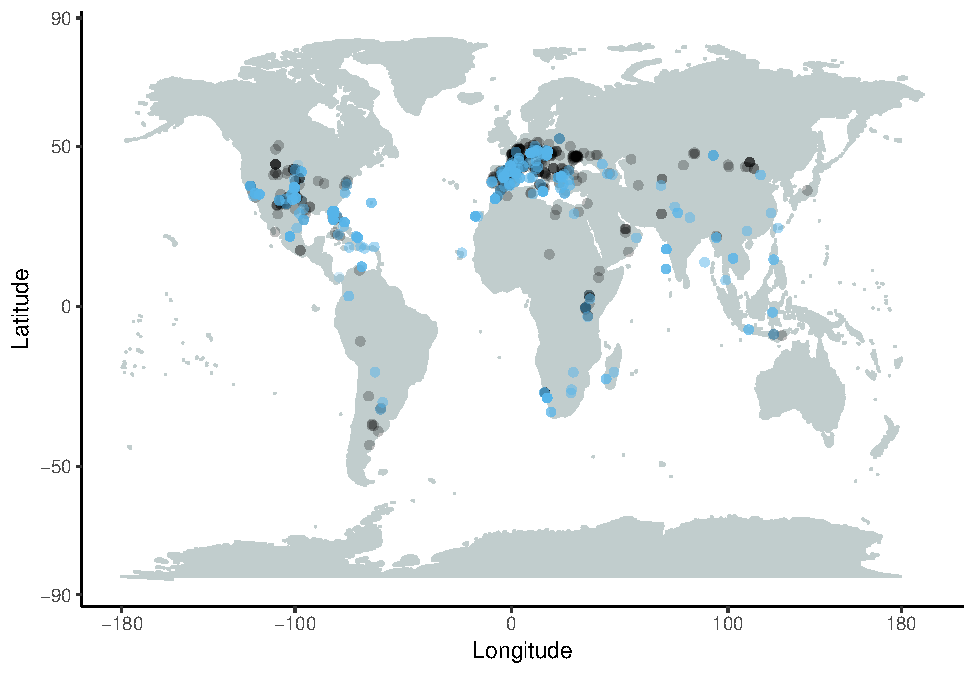
\includegraphics{MA_JJ_files/figure-latex/MapFossilOccurrences-1.pdf}
\caption{Map displaying all fossil occurrences of testudinids, with
color indicating whether relevant literature was available (black if
not) and if it was, whether body size data was available or not (yes and
no, respectively).}
\end{figure}

\newpage

\subsection{body size of testudinidae}\label{body-size-of-testudinidae}

\begin{figure}[htbp]
\centering
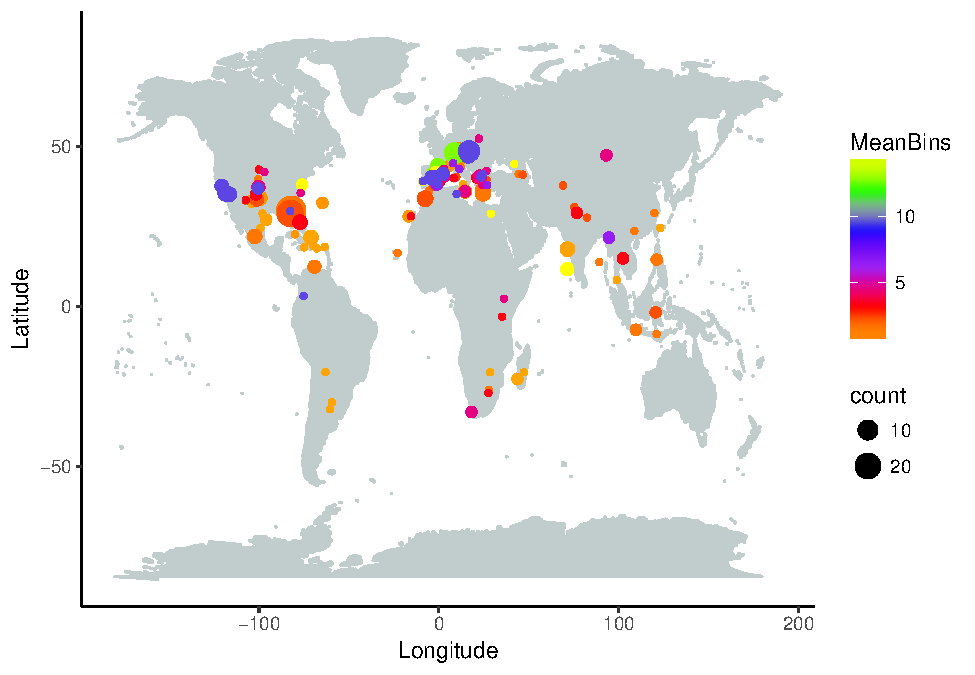
\includegraphics{MA_JJ_files/figure-latex/MapCL-1.pdf}
\caption{Map displaying all localities for which body size data for
testudinids was available in the literature. Size of points denotes
sample size, color denotes approximate age.}
\end{figure}

\begin{longtable}[]{@{}llrr@{}}
\caption{Overview over fossil species per time bin, with sample size and
mean CL.}\tabularnewline
\toprule
EpochBins & Taxon & n & meanCL\tabularnewline
\midrule
\endfirsthead
\toprule
EpochBins & Taxon & n & meanCL\tabularnewline
\midrule
\endhead
Upper Pleistocene & Centrochelys robusta & 1 & 850.0000\tabularnewline
Upper Pleistocene & Chelonoidis denticulata & 1 &
616.0000\tabularnewline
Upper Pleistocene & Chelonoidis lutzae & 1 & 830.0000\tabularnewline
Upper Pleistocene & Chelonoidis marcanoi & 4 & 672.2500\tabularnewline
Upper Pleistocene & Chelonoidis monensis & 1 & 500.0000\tabularnewline
Upper Pleistocene & Chelonoidis sombrerensis & 1 &
990.0000\tabularnewline
Upper Pleistocene & Chelonoidis sp. & 3 & 666.6667\tabularnewline
Upper Pleistocene & Eurotestudo hermanni & 1 & 187.0000\tabularnewline
Upper Pleistocene & gen. indet. & 1 & 813.0000\tabularnewline
Upper Pleistocene & Geochelone sp. & 2 & 475.0000\tabularnewline
Upper Pleistocene & Gopherus agassizi & 1 & 252.0000\tabularnewline
Upper Pleistocene & Gopherus polyphemus & 20 & 292.9700\tabularnewline
Upper Pleistocene & Gopherus praecedens & 1 & 360.0000\tabularnewline
Upper Pleistocene & Hesperotestudo crassiscutata & 6 &
435.1667\tabularnewline
Upper Pleistocene & Hesperotestudo incisa & 1 & 232.7600\tabularnewline
Upper Pleistocene & Hesperotestudo sp. & 2 & 806.5000\tabularnewline
Upper Pleistocene & Hesperotestudo wilsoni & 1 & 226.0000\tabularnewline
Upper Pleistocene & Indotestudo elongata & 1 & 270.0000\tabularnewline
Middle Pleistocene & Centrochelys burchardi & 4 &
722.5000\tabularnewline
Middle Pleistocene & Chelonoidis cubensis & 1 & 1139.0000\tabularnewline
Middle Pleistocene & Eurotestudo aff. hermanni & 2 &
187.0000\tabularnewline
Middle Pleistocene & Eurotestudo hermanni & 2 & 204.0500\tabularnewline
Middle Pleistocene & Geochelone sp. & 1 & 170.0000\tabularnewline
Middle Pleistocene & Gopherus agassizi & 1 & 445.0000\tabularnewline
Middle Pleistocene & Gopherus laticaudatus & 1 & 375.0000\tabularnewline
Middle Pleistocene & Gopherus polyphemus & 31 & 300.4316\tabularnewline
Middle Pleistocene & Hesperotestudo bermudae & 2 &
385.0000\tabularnewline
Middle Pleistocene & Hesperotestudo equicomes & 1 &
340.0000\tabularnewline
Middle Pleistocene & Hesperotestudo sp. & 2 & 1650.0000\tabularnewline
Middle Pleistocene & Testudo kenitrensis & 1 & 132.0000\tabularnewline
Middle Pleistocene & Testudo lunellensis & 4 & 215.4250\tabularnewline
Lower Pleistocene & Centrochelys atlantica & 1 & 400.0000\tabularnewline
Lower Pleistocene & Centrochelys robusta & 3 & 883.3333\tabularnewline
Lower Pleistocene & Cheirogaster cf.~gymnesica & 1 &
789.0000\tabularnewline
Lower Pleistocene & Cheirogaster sp. & 1 & 925.0000\tabularnewline
Lower Pleistocene & Chelonoidis sp. & 3 & 716.6667\tabularnewline
Lower Pleistocene & Eurotestudo globosa & 1 & 263.0000\tabularnewline
Lower Pleistocene & Eurotestudo hermanni & 2 & 205.0000\tabularnewline
Lower Pleistocene & gen. indet. & 1 & 900.0000\tabularnewline
Lower Pleistocene & Geochelone sp. & 1 & 340.0000\tabularnewline
Lower Pleistocene & Gopherus berlandieri & 2 & 225.6500\tabularnewline
Lower Pleistocene & Gopherus flavomarginatus & 1 &
450.0000\tabularnewline
Lower Pleistocene & Gopherus pertenuis & 1 & 1050.0000\tabularnewline
Lower Pleistocene & Gopherus polyphemus & 3 & 254.4667\tabularnewline
Lower Pleistocene & Gopherus sp. & 6 & 233.9667\tabularnewline
Lower Pleistocene & Hesperotestudo crassiscutata & 5 &
285.6000\tabularnewline
Lower Pleistocene & Hesperotestudo incisa & 7 & 234.6286\tabularnewline
Lower Pleistocene & Hesperotestudo mlynarskii & 2 &
184.2500\tabularnewline
Lower Pleistocene & Hesperotestudo sp. & 1 & 1500.0000\tabularnewline
Lower Pleistocene & Hesperotestudo turgida & 1 & 230.0000\tabularnewline
Lower Pleistocene & Megalochelys sondaari & 2 & 909.0000\tabularnewline
Lower Pleistocene & Megalochelys sp. & 3 & 1130.4667\tabularnewline
Lower Pleistocene & Psammobates antiquorum & 1 & 107.8000\tabularnewline
Lower Pleistocene & Testudo changshanesis & 1 & 330.0000\tabularnewline
Lower Pleistocene & Testudo graeca & 1 & 195.0000\tabularnewline
Lower Pleistocene & Testudo hermanni & 2 & 176.5500\tabularnewline
Lower Pleistocene & Testudo marginata & 3 & 270.0000\tabularnewline
Lower Pleistocene & Titanochelon gymnesica & 1 &
1300.0000\tabularnewline
Gelasian & Centrochelys marocana & 1 & 2050.0000\tabularnewline
Gelasian & Eurotestudo cf.~hermanni & 1 & 150.0000\tabularnewline
Gelasian & Gopherus sp. & 15 & 185.7467\tabularnewline
Gelasian & Hesperotestudo campester & 1 & 1000.0000\tabularnewline
Gelasian & Hesperotestudo sp. & 1 & 1000.0000\tabularnewline
Gelasian & Manouria punjabiensis & 1 & 900.0000\tabularnewline
Gelasian & Megalochelys atlas & 3 & 1683.3333\tabularnewline
Gelasian & Testudo aff. kenitrensis & 1 & 142.0000\tabularnewline
Gelasian & Testudo oughlamensis & 1 & 120.0000\tabularnewline
Gelasian & Testudo ranovi & 1 & 200.0000\tabularnewline
Gelasian & Testudo sp. & 2 & 192.0000\tabularnewline
Gelasian & Testudo transcaucasia & 1 & 150.0000\tabularnewline
Gelasian & Titanochelon aff. schafferi & 1 & 1860.0000\tabularnewline
Gelasian & Titanochelon sp. & 1 & 1420.0000\tabularnewline
Piacencian & ``Aldabrachelys'' laetoliensis & 1 &
1000.0000\tabularnewline
Piacencian & Aldabrachelys ? sp. & 2 & 1500.0000\tabularnewline
Piacencian & Centrochelys vulcanica & 1 & 610.0000\tabularnewline
Piacencian & Chelonoidis alburyorum & 4 & 442.7500\tabularnewline
Piacencian & Gopherus canyonensis & 1 & 885.5000\tabularnewline
Piacencian & Hesperotestudo johnstoni & 1 & 235.0000\tabularnewline
Piacencian & Hesperotestudo oelrichi & 1 & 283.8000\tabularnewline
Piacencian & Hesperotestudo riggsi & 2 & 180.5000\tabularnewline
Piacencian & Hesperotestudo sp. & 1 & 176.0000\tabularnewline
Piacencian & Homopus fenestratus & 1 & 90.0000\tabularnewline
Piacencian & Megalochelys atlas & 2 & 1600.0000\tabularnewline
Piacencian & Testudo brevitesta & 2 & 232.5000\tabularnewline
Piacencian & Testudo pecorinii & 1 & 225.0000\tabularnewline
Piacencian & Titanochelon sp. & 1 & 520.0000\tabularnewline
Zanclean & Caudochelys rexroadensis & 2 & 805.5000\tabularnewline
Zanclean & Centrochelys robusta & 3 & 913.3333\tabularnewline
Zanclean & Cheirogaster gymnesica & 1 & 739.0000\tabularnewline
Zanclean & Ergilemys oskarkuhni & 2 & 209.0000\tabularnewline
Zanclean & Geochelone crassa & 1 & 865.0000\tabularnewline
Zanclean & Geochelone s. l. & 1 & 1750.0000\tabularnewline
Zanclean & Geochelone sp. & 2 & 528.0000\tabularnewline
Zanclean & Geochelone stromeri & 2 & 387.5000\tabularnewline
Zanclean & Hesperotestudo riggsi & 1 & 195.8000\tabularnewline
Zanclean & Testudo cf.~graeca & 1 & 185.0000\tabularnewline
Zanclean & Testudo sp. & 4 & 1675.0000\tabularnewline
Zanclean & Titanochelon bacharidisi & 4 & 1040.0000\tabularnewline
Zanclean & Titanochelon perpiniana & 1 & 1140.0000\tabularnewline
Zanclean & Titanochelon schafferi & 1 & 2500.0000\tabularnewline
Messinian & Hesperotestudo orthopygia & 2 & 941.0000\tabularnewline
Messinian & Megalochelys atlas & 2 & 1950.0000\tabularnewline
Messinian & Testudo amiatae & 1 & 140.0000\tabularnewline
Messinian & Testudo graeca & 2 & 183.5000\tabularnewline
Messinian & Testudo sp. & 1 & 200.0000\tabularnewline
Messinian & Titanochelon bolivari & 1 & 1150.0000\tabularnewline
Messinian & Titanochelon schafferi & 1 & 1850.0000\tabularnewline
Tortonian & ``Hadrianus sp.'' & 1 & 1000.0000\tabularnewline
Tortonian & Cheirogaster richardi & 1 & 1155.0000\tabularnewline
Tortonian & Cheirogaster sp. & 2 & 1355.0000\tabularnewline
Tortonian & gen. indet. & 3 & 660.0000\tabularnewline
Tortonian & Geochelone hesterna & 1 & 278.0000\tabularnewline
Tortonian & Geochelone sp. & 2 & 973.0000\tabularnewline
Tortonian & Gopherus ? sp. & 1 & 500.0000\tabularnewline
Tortonian & Gopherus mohavetus & 5 & 324.8000\tabularnewline
Tortonian & Hesperotestudo alleni & 1 & 240.9000\tabularnewline
Tortonian & Hesperotestudo riggsi & 2 & 159.5000\tabularnewline
Tortonian & Hesperotestudo sp. & 1 & 1200.0000\tabularnewline
Tortonian & Paleotestudo sp. & 3 & 233.6667\tabularnewline
Tortonian & Testudo burgenlandica & 2 & 193.5000\tabularnewline
Tortonian & Testudo catalaunica & 4 & 157.0000\tabularnewline
Tortonian & Testudo cf.~promarginata & 5 & 250.0000\tabularnewline
Tortonian & Testudo graeca & 1 & 210.0000\tabularnewline
Tortonian & Testudo s. s. & 1 & 189.0000\tabularnewline
Tortonian & Testudo sp. & 7 & 243.1571\tabularnewline
Tortonian & Titanochelon bolivari & 1 & 1300.0000\tabularnewline
Tortonian & Titanochelon cf.~bolivari & 1 & 1500.0000\tabularnewline
Serravallian & Cheirogaster sp. & 2 & 1250.0000\tabularnewline
Serravallian & gen. indet. & 1 & 270.0000\tabularnewline
Serravallian & Gopherus ? sp. & 1 & 500.0000\tabularnewline
Serravallian & Paleotestudo antiqua & 18 & 203.0556\tabularnewline
Serravallian & Paleotestudo cf.~sp. & 1 & 270.0000\tabularnewline
Serravallian & Testudo catalaunica & 1 & 232.0000\tabularnewline
Serravallian & Testudo steinheimensis & 2 & 169.3500\tabularnewline
Serravallian & Titanochelon bolivari & 1 & 1353.0000\tabularnewline
Langhian & Caudochelys ducateli & 1 & 339.9000\tabularnewline
Langhian & Chelonoidis sp. & 3 & 553.3333\tabularnewline
Langhian & Ergilemys sp. & 1 & 1000.0000\tabularnewline
Langhian & gen. indet. & 1 & 1000.0000\tabularnewline
Langhian & Paleotestudo antiqua & 1 & 275.0000\tabularnewline
Langhian & Paleotestudo cf.~sp. & 1 & 270.0000\tabularnewline
Langhian & Testudo kalksburgensis & 1 & 275.0000\tabularnewline
Langhian & Testudo sp. & 1 & 400.0000\tabularnewline
Langhian & Titanochelon bolivari & 2 & 1175.0000\tabularnewline
Langhian & Titanochelon cf.~bolivari & 2 & 1450.0000\tabularnewline
Burdigalian/Aquitanian & Caudochelys williamsi & 1 &
334.0000\tabularnewline
Burdigalian/Aquitanian & gen. indet. & 1 & 270.0000\tabularnewline
Burdigalian/Aquitanian & Geochelone sp. & 2 & 900.0000\tabularnewline
Burdigalian/Aquitanian & Geochelone tedwhitei & 2 &
405.0000\tabularnewline
Burdigalian/Aquitanian & Impregnochelys pachytectis & 1 &
620.0000\tabularnewline
Burdigalian/Aquitanian & Mesocherus orangeus & 5 &
180.0000\tabularnewline
Burdigalian/Aquitanian & Namibchersus aff. namaquensis & 3 &
696.6667\tabularnewline
Burdigalian/Aquitanian & Namibchersus namaquensis & 6 &
428.8333\tabularnewline
Burdigalian/Aquitanian & Paleotestudo cf.~antiqua & 1 &
113.0000\tabularnewline
Burdigalian/Aquitanian & Paleotestudo sp. & 1 & 179.3000\tabularnewline
Burdigalian/Aquitanian & Testudo kalksburgensis & 2 &
227.5000\tabularnewline
Burdigalian/Aquitanian & Testudo promarginata & 3 &
281.5667\tabularnewline
Burdigalian/Aquitanian & Testudo rectogularis & 1 &
213.0000\tabularnewline
Burdigalian/Aquitanian & Titanochelon cf.~perpiniana & 1 &
1001.0000\tabularnewline
\bottomrule
\end{longtable}

\begin{longtable}[]{@{}lrr@{}}
\caption{General overview over fossil species, with sample size and mean
CL}\tabularnewline
\toprule
Taxon & n & meanCL\tabularnewline
\midrule
\endfirsthead
\toprule
Taxon & n & meanCL\tabularnewline
\midrule
\endhead
``Aldabrachelys'' laetoliensis & 1 & 1000.0000\tabularnewline
``Hadrianus sp.'' & 1 & 1000.0000\tabularnewline
Aldabrachelys ? sp. & 2 & 1500.0000\tabularnewline
Caudochelys ducateli & 1 & 339.9000\tabularnewline
Caudochelys rexroadensis & 2 & 805.5000\tabularnewline
Caudochelys williamsi & 1 & 334.0000\tabularnewline
Centrochelys atlantica & 1 & 400.0000\tabularnewline
Centrochelys burchardi & 4 & 722.5000\tabularnewline
Centrochelys marocana & 1 & 2050.0000\tabularnewline
Centrochelys robusta & 7 & 891.4286\tabularnewline
Centrochelys vulcanica & 1 & 610.0000\tabularnewline
Cheirogaster cf.~gymnesica & 1 & 789.0000\tabularnewline
Cheirogaster gymnesica & 1 & 739.0000\tabularnewline
Cheirogaster richardi & 1 & 1155.0000\tabularnewline
Cheirogaster sp. & 5 & 1227.0000\tabularnewline
Chelonoidis alburyorum & 4 & 442.7500\tabularnewline
Chelonoidis cubensis & 1 & 1139.0000\tabularnewline
Chelonoidis denticulata & 1 & 616.0000\tabularnewline
Chelonoidis lutzae & 1 & 830.0000\tabularnewline
Chelonoidis marcanoi & 4 & 672.2500\tabularnewline
Chelonoidis monensis & 1 & 500.0000\tabularnewline
Chelonoidis sombrerensis & 1 & 990.0000\tabularnewline
Chelonoidis sp. & 9 & 645.5556\tabularnewline
Ergilemys oskarkuhni & 2 & 209.0000\tabularnewline
Ergilemys sp. & 1 & 1000.0000\tabularnewline
Eurotestudo aff. hermanni & 2 & 187.0000\tabularnewline
Eurotestudo cf.~hermanni & 1 & 150.0000\tabularnewline
Eurotestudo globosa & 1 & 263.0000\tabularnewline
Eurotestudo hermanni & 5 & 201.0200\tabularnewline
gen. indet. & 8 & 654.1250\tabularnewline
Geochelone crassa & 1 & 865.0000\tabularnewline
Geochelone hesterna & 1 & 278.0000\tabularnewline
Geochelone s. l. & 1 & 1750.0000\tabularnewline
Geochelone sp. & 10 & 626.2000\tabularnewline
Geochelone stromeri & 2 & 387.5000\tabularnewline
Geochelone tedwhitei & 2 & 405.0000\tabularnewline
Gopherus ? sp. & 2 & 500.0000\tabularnewline
Gopherus agassizi & 2 & 348.5000\tabularnewline
Gopherus berlandieri & 2 & 225.6500\tabularnewline
Gopherus canyonensis & 1 & 885.5000\tabularnewline
Gopherus flavomarginatus & 1 & 450.0000\tabularnewline
Gopherus laticaudatus & 1 & 375.0000\tabularnewline
Gopherus mohavetus & 5 & 324.8000\tabularnewline
Gopherus pertenuis & 1 & 1050.0000\tabularnewline
Gopherus polyphemus & 54 & 295.1144\tabularnewline
Gopherus praecedens & 1 & 360.0000\tabularnewline
Gopherus sp. & 21 & 199.5238\tabularnewline
Hesperotestudo alleni & 1 & 240.9000\tabularnewline
Hesperotestudo bermudae & 2 & 385.0000\tabularnewline
Hesperotestudo campester & 1 & 1000.0000\tabularnewline
Hesperotestudo crassiscutata & 11 & 367.1818\tabularnewline
Hesperotestudo equicomes & 1 & 340.0000\tabularnewline
Hesperotestudo incisa & 8 & 234.3950\tabularnewline
Hesperotestudo johnstoni & 1 & 235.0000\tabularnewline
Hesperotestudo mlynarskii & 2 & 184.2500\tabularnewline
Hesperotestudo oelrichi & 1 & 283.8000\tabularnewline
Hesperotestudo orthopygia & 2 & 941.0000\tabularnewline
Hesperotestudo riggsi & 5 & 175.1600\tabularnewline
Hesperotestudo sp. & 8 & 1098.6250\tabularnewline
Hesperotestudo turgida & 1 & 230.0000\tabularnewline
Hesperotestudo wilsoni & 1 & 226.0000\tabularnewline
Homopus fenestratus & 1 & 90.0000\tabularnewline
Impregnochelys pachytectis & 1 & 620.0000\tabularnewline
Indotestudo elongata & 1 & 270.0000\tabularnewline
Manouria punjabiensis & 1 & 900.0000\tabularnewline
Megalochelys atlas & 7 & 1735.7143\tabularnewline
Megalochelys sondaari & 2 & 909.0000\tabularnewline
Megalochelys sp. & 3 & 1130.4667\tabularnewline
Mesocherus orangeus & 5 & 180.0000\tabularnewline
Namibchersus aff. namaquensis & 3 & 696.6667\tabularnewline
Namibchersus namaquensis & 6 & 428.8333\tabularnewline
Paleotestudo antiqua & 19 & 206.8421\tabularnewline
Paleotestudo cf.~antiqua & 1 & 113.0000\tabularnewline
Paleotestudo cf.~sp. & 2 & 270.0000\tabularnewline
Paleotestudo sp. & 4 & 220.0750\tabularnewline
Psammobates antiquorum & 1 & 107.8000\tabularnewline
Testudo aff. kenitrensis & 1 & 142.0000\tabularnewline
Testudo amiatae & 1 & 140.0000\tabularnewline
Testudo brevitesta & 2 & 232.5000\tabularnewline
Testudo burgenlandica & 2 & 193.5000\tabularnewline
Testudo catalaunica & 5 & 172.0000\tabularnewline
Testudo cf.~graeca & 1 & 185.0000\tabularnewline
Testudo cf.~promarginata & 5 & 250.0000\tabularnewline
Testudo changshanesis & 1 & 330.0000\tabularnewline
Testudo graeca & 4 & 193.0000\tabularnewline
Testudo hermanni & 2 & 176.5500\tabularnewline
Testudo kalksburgensis & 3 & 243.3333\tabularnewline
Testudo kenitrensis & 1 & 132.0000\tabularnewline
Testudo lunellensis & 4 & 215.4250\tabularnewline
Testudo marginata & 3 & 270.0000\tabularnewline
Testudo oughlamensis & 1 & 120.0000\tabularnewline
Testudo pecorinii & 1 & 225.0000\tabularnewline
Testudo promarginata & 3 & 281.5667\tabularnewline
Testudo ranovi & 1 & 200.0000\tabularnewline
Testudo rectogularis & 1 & 213.0000\tabularnewline
Testudo s. s. & 1 & 189.0000\tabularnewline
Testudo sp. & 15 & 625.7400\tabularnewline
Testudo steinheimensis & 2 & 169.3500\tabularnewline
Testudo transcaucasia & 1 & 150.0000\tabularnewline
Titanochelon aff. schafferi & 1 & 1860.0000\tabularnewline
Titanochelon bacharidisi & 4 & 1040.0000\tabularnewline
Titanochelon bolivari & 5 & 1230.6000\tabularnewline
Titanochelon cf.~bolivari & 3 & 1466.6667\tabularnewline
Titanochelon cf.~perpiniana & 1 & 1001.0000\tabularnewline
Titanochelon gymnesica & 1 & 1300.0000\tabularnewline
Titanochelon perpiniana & 1 & 1140.0000\tabularnewline
Titanochelon schafferi & 2 & 2175.0000\tabularnewline
Titanochelon sp. & 2 & 970.0000\tabularnewline
\bottomrule
\end{longtable}

\begin{longtable}[]{@{}llrr@{}}
\caption{Overview over genera (modern and fossil) per time bin, with
sample sizes and mean CL.}\tabularnewline
\toprule
EpochBins & Genus & n & meanCL\tabularnewline
\midrule
\endfirsthead
\toprule
EpochBins & Genus & n & meanCL\tabularnewline
\midrule
\endhead
Modern & Aldabrachelys & 12 & 974.5833\tabularnewline
Modern & Astrochelys & 14 & 366.2143\tabularnewline
Modern & Centrochelys & 3 & 493.3333\tabularnewline
Modern & Chelonoidis & 45 & 531.5178\tabularnewline
Modern & Chersina & 15 & 176.2667\tabularnewline
Modern & Cylindraspis & 5 & 724.0000\tabularnewline
Modern & Geochelone & 8 & 252.1250\tabularnewline
Modern & Gopherus & 23 & 302.4839\tabularnewline
Modern & Hesperotestudo & 1 & 250.0000\tabularnewline
Modern & Homopus & 7 & 139.2857\tabularnewline
Modern & Indotestudo & 16 & 242.9875\tabularnewline
Modern & Kinixys & 15 & 213.0667\tabularnewline
Modern & Malacochersus & 2 & 166.5000\tabularnewline
Modern & Manouria & 9 & 380.7778\tabularnewline
Modern & Psammobates & 17 & 113.4118\tabularnewline
Modern & Pyxis & 16 & 124.1875\tabularnewline
Modern & Stigmochelys & 6 & 405.3333\tabularnewline
Modern & Testudo & 39 & 197.5436\tabularnewline
Upper Pleistocene & Centrochelys & 1 & 850.0000\tabularnewline
Upper Pleistocene & Chelonoidis & 11 & 693.1818\tabularnewline
Upper Pleistocene & Eurotestudo & 1 & 187.0000\tabularnewline
Upper Pleistocene & gen. & 1 & 813.0000\tabularnewline
Upper Pleistocene & Geochelone & 2 & 475.0000\tabularnewline
Upper Pleistocene & Gopherus & 22 & 294.1545\tabularnewline
Upper Pleistocene & Hesperotestudo & 10 & 468.2760\tabularnewline
Upper Pleistocene & Indotestudo & 1 & 270.0000\tabularnewline
Middle Pleistocene & Centrochelys & 4 & 722.5000\tabularnewline
Middle Pleistocene & Chelonoidis & 1 & 1139.0000\tabularnewline
Middle Pleistocene & Eurotestudo & 4 & 195.5250\tabularnewline
Middle Pleistocene & Geochelone & 1 & 170.0000\tabularnewline
Middle Pleistocene & Gopherus & 33 & 307.0721\tabularnewline
Middle Pleistocene & Hesperotestudo & 5 & 882.0000\tabularnewline
Middle Pleistocene & Testudo & 5 & 198.7400\tabularnewline
Lower Pleistocene & Centrochelys & 4 & 762.5000\tabularnewline
Lower Pleistocene & Cheirogaster & 2 & 857.0000\tabularnewline
Lower Pleistocene & Chelonoidis & 3 & 716.6667\tabularnewline
Lower Pleistocene & Eurotestudo & 4 & 201.5250\tabularnewline
Lower Pleistocene & gen. & 1 & 900.0000\tabularnewline
Lower Pleistocene & Geochelone & 1 & 340.0000\tabularnewline
Lower Pleistocene & Gopherus & 13 & 316.8077\tabularnewline
Lower Pleistocene & Hesperotestudo & 16 & 323.0562\tabularnewline
Lower Pleistocene & Megalochelys & 5 & 1041.8800\tabularnewline
Lower Pleistocene & Psammobates & 1 & 107.8000\tabularnewline
Lower Pleistocene & Testudo & 6 & 259.1667\tabularnewline
Lower Pleistocene & Titanochelon & 1 & 1300.0000\tabularnewline
Gelasian & Centrochelys & 1 & 2050.0000\tabularnewline
Gelasian & Eurotestudo & 1 & 150.0000\tabularnewline
Gelasian & Gopherus & 15 & 185.7467\tabularnewline
Gelasian & Hesperotestudo & 2 & 1000.0000\tabularnewline
Gelasian & Manouria & 1 & 900.0000\tabularnewline
Gelasian & Megalochelys & 3 & 1683.3333\tabularnewline
Gelasian & Testudo & 6 & 166.0000\tabularnewline
Gelasian & Titanochelon & 2 & 1640.0000\tabularnewline
Piacencian & Aldabrachelys & 3 & 1333.3333\tabularnewline
Piacencian & Centrochelys & 1 & 610.0000\tabularnewline
Piacencian & Chelonoidis & 4 & 442.7500\tabularnewline
Piacencian & Gopherus & 1 & 885.5000\tabularnewline
Piacencian & Hesperotestudo & 5 & 211.1600\tabularnewline
Piacencian & Homopus & 1 & 90.0000\tabularnewline
Piacencian & Megalochelys & 2 & 1600.0000\tabularnewline
Piacencian & Testudo & 3 & 230.0000\tabularnewline
Piacencian & Titanochelon & 1 & 520.0000\tabularnewline
Zanclean & Caudochelys & 2 & 805.5000\tabularnewline
Zanclean & Centrochelys & 3 & 913.3333\tabularnewline
Zanclean & Cheirogaster & 1 & 739.0000\tabularnewline
Zanclean & Ergilemys & 2 & 209.0000\tabularnewline
Zanclean & Geochelone & 6 & 741.0000\tabularnewline
Zanclean & Hesperotestudo & 1 & 195.8000\tabularnewline
Zanclean & Testudo & 5 & 1377.0000\tabularnewline
Zanclean & Titanochelon & 6 & 1300.0000\tabularnewline
Messinian & Hesperotestudo & 2 & 941.0000\tabularnewline
Messinian & Megalochelys & 2 & 1950.0000\tabularnewline
Messinian & Testudo & 4 & 176.7500\tabularnewline
Messinian & Titanochelon & 2 & 1500.0000\tabularnewline
Tortonian & ``Hadrianus'' & 1 & 1000.0000\tabularnewline
Tortonian & Cheirogaster & 3 & 1288.3333\tabularnewline
Tortonian & gen. & 3 & 660.0000\tabularnewline
Tortonian & Geochelone & 3 & 741.3333\tabularnewline
Tortonian & Gopherus & 6 & 354.0000\tabularnewline
Tortonian & Hesperotestudo & 4 & 439.9750\tabularnewline
Tortonian & Paleotestudo & 3 & 233.6667\tabularnewline
Tortonian & Testudo & 20 & 218.3050\tabularnewline
Tortonian & Titanochelon & 2 & 1400.0000\tabularnewline
Serravallian & Cheirogaster & 2 & 1250.0000\tabularnewline
Serravallian & gen. & 1 & 270.0000\tabularnewline
Serravallian & Gopherus & 1 & 500.0000\tabularnewline
Serravallian & Paleotestudo & 19 & 206.5789\tabularnewline
Serravallian & Testudo & 3 & 190.2333\tabularnewline
Serravallian & Titanochelon & 1 & 1353.0000\tabularnewline
Langhian & Caudochelys & 1 & 339.9000\tabularnewline
Langhian & Chelonoidis & 3 & 553.3333\tabularnewline
Langhian & Ergilemys & 1 & 1000.0000\tabularnewline
Langhian & gen. & 1 & 1000.0000\tabularnewline
Langhian & Paleotestudo & 2 & 272.5000\tabularnewline
Langhian & Testudo & 2 & 337.5000\tabularnewline
Langhian & Titanochelon & 4 & 1312.5000\tabularnewline
Burdigalian/Aquitanian & Caudochelys & 1 & 334.0000\tabularnewline
Burdigalian/Aquitanian & gen. & 1 & 270.0000\tabularnewline
Burdigalian/Aquitanian & Geochelone & 4 & 652.5000\tabularnewline
Burdigalian/Aquitanian & Impregnochelys & 1 & 620.0000\tabularnewline
Burdigalian/Aquitanian & Mesocherus & 5 & 180.0000\tabularnewline
Burdigalian/Aquitanian & Namibchersus & 9 & 518.1111\tabularnewline
Burdigalian/Aquitanian & Paleotestudo & 2 & 146.1500\tabularnewline
Burdigalian/Aquitanian & Testudo & 6 & 252.1167\tabularnewline
Burdigalian/Aquitanian & Titanochelon & 1 & 1001.0000\tabularnewline
\bottomrule
\end{longtable}

\begin{longtable}[]{@{}lrr@{}}
\caption{General overview over genera, with sample sizes and mean
CL.}\tabularnewline
\toprule
Genus & n & meanCL\tabularnewline
\midrule
\endfirsthead
\toprule
Genus & n & meanCL\tabularnewline
\midrule
\endhead
``Hadrianus'' & 1 & 1000.0000\tabularnewline
Aldabrachelys & 15 & 1046.3333\tabularnewline
Astrochelys & 14 & 366.2143\tabularnewline
Caudochelys & 4 & 571.2250\tabularnewline
Centrochelys & 17 & 804.1176\tabularnewline
Cheirogaster & 8 & 1102.2500\tabularnewline
Chelonoidis & 67 & 571.0940\tabularnewline
Chersina & 15 & 176.2667\tabularnewline
Cylindraspis & 5 & 724.0000\tabularnewline
Ergilemys & 3 & 472.6667\tabularnewline
Eurotestudo & 10 & 192.5200\tabularnewline
gen. & 8 & 654.1250\tabularnewline
Geochelone & 25 & 510.2800\tabularnewline
Gopherus & 114 & 298.0361\tabularnewline
Hesperotestudo & 46 & 465.3296\tabularnewline
Homopus & 8 & 133.1250\tabularnewline
Impregnochelys & 1 & 620.0000\tabularnewline
Indotestudo & 17 & 244.5765\tabularnewline
Kinixys & 15 & 213.0667\tabularnewline
Malacochersus & 2 & 166.5000\tabularnewline
Manouria & 10 & 432.7000\tabularnewline
Megalochelys & 12 & 1446.6167\tabularnewline
Mesocherus & 5 & 180.0000\tabularnewline
Namibchersus & 9 & 518.1111\tabularnewline
Paleotestudo & 26 & 210.1269\tabularnewline
Psammobates & 18 & 113.1000\tabularnewline
Pyxis & 16 & 124.1875\tabularnewline
Stigmochelys & 6 & 405.3333\tabularnewline
Testudo & 99 & 269.2465\tabularnewline
Titanochelon & 20 & 1315.2000\tabularnewline
\bottomrule
\end{longtable}

\newpage

\section{Sampling Accumulation
Curves}\label{sampling-accumulation-curves}

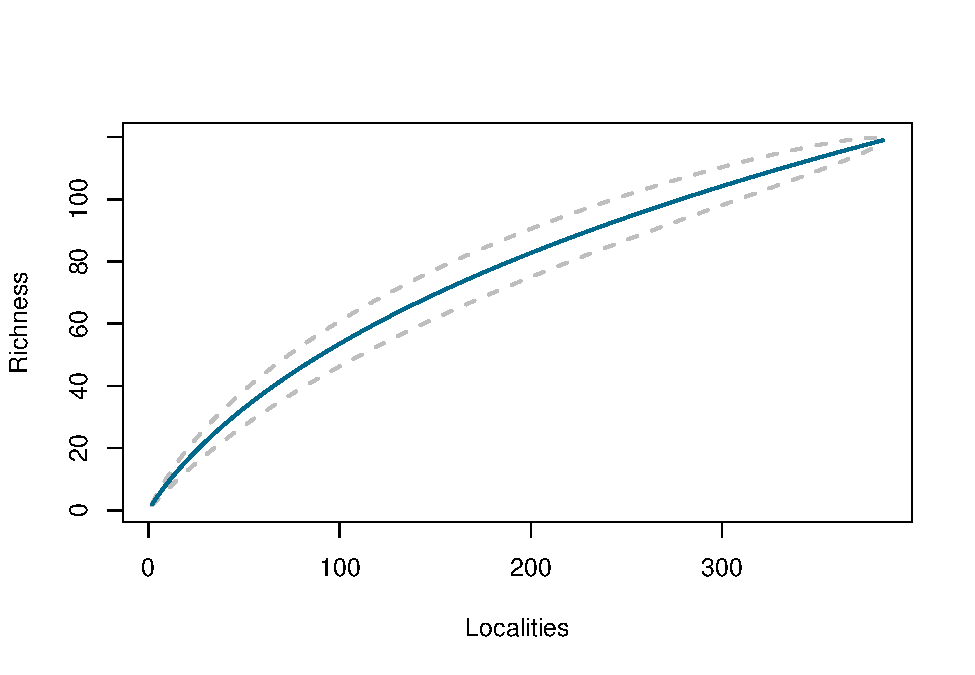
\includegraphics{MA_JJ_files/figure-latex/SACSpecies-1.pdf}
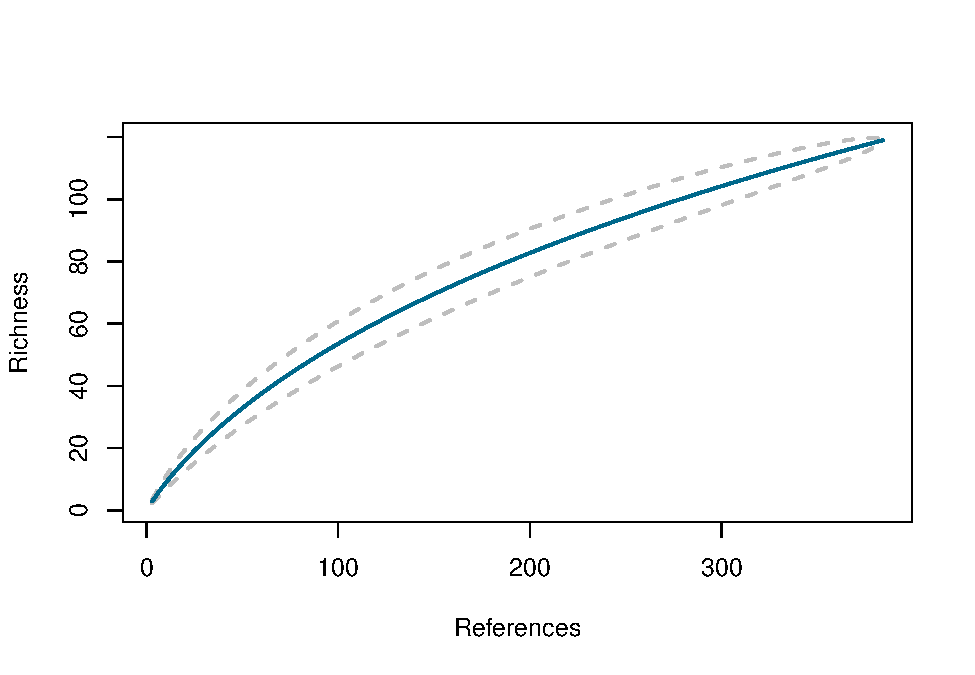
\includegraphics{MA_JJ_files/figure-latex/SACSpecies-2.pdf}

\begin{figure}[htbp]
\centering
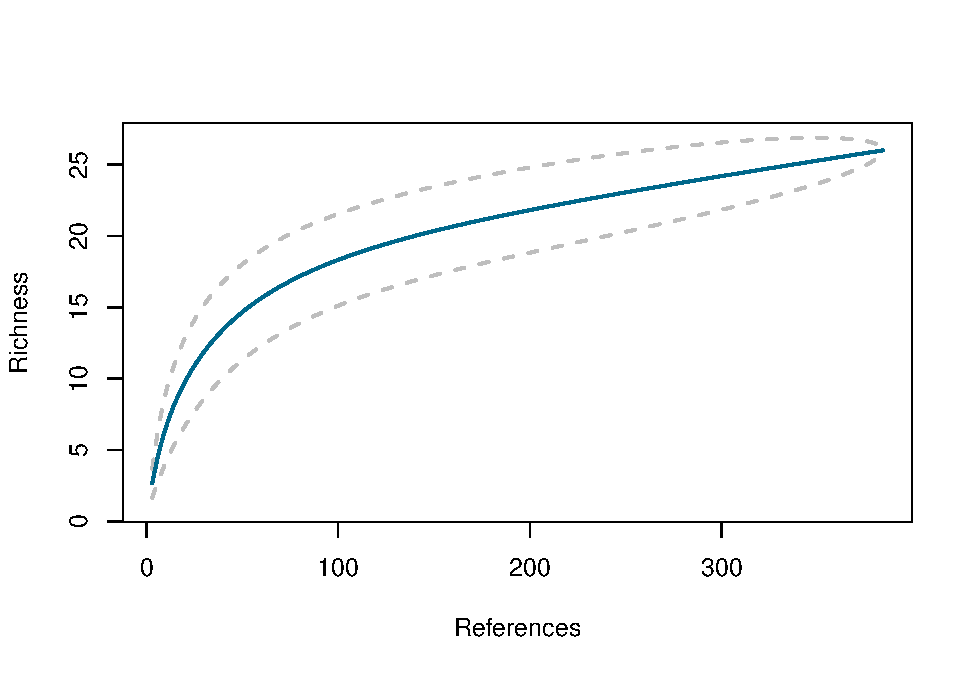
\includegraphics{MA_JJ_files/figure-latex/SACGenera-1.pdf}
\caption{Sampling Accumulation Curve of fossil genera per reference}
\end{figure}

\begin{figure}[htbp]
\centering
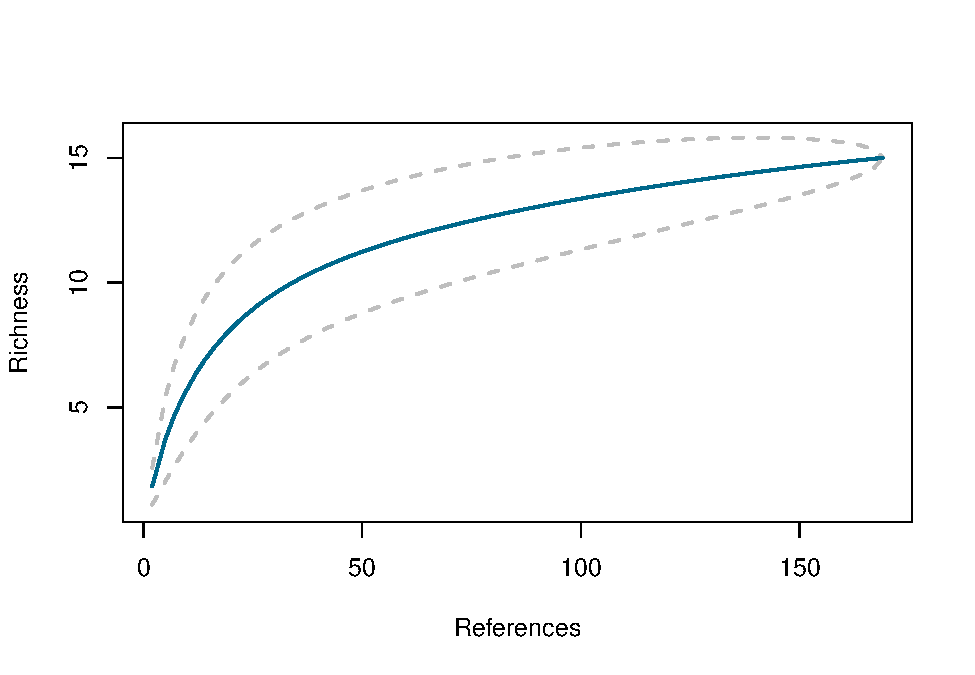
\includegraphics{MA_JJ_files/figure-latex/SACGEurasia-1.pdf}
\caption{Sampling Accumulation Curve of fossil genera per reference,
Eurasia}
\end{figure}

\begin{figure}[htbp]
\centering
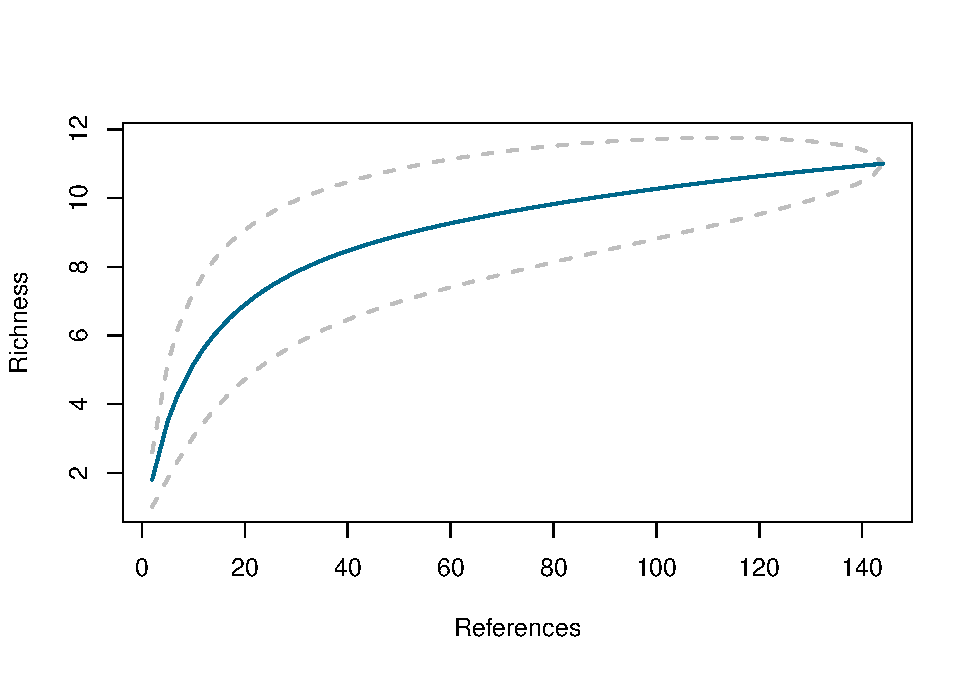
\includegraphics{MA_JJ_files/figure-latex/SACGEurope-1.pdf}
\caption{Sampling Accumulation Curve of fossil genera per reference,
Europe}
\end{figure}

\begin{figure}[htbp]
\centering
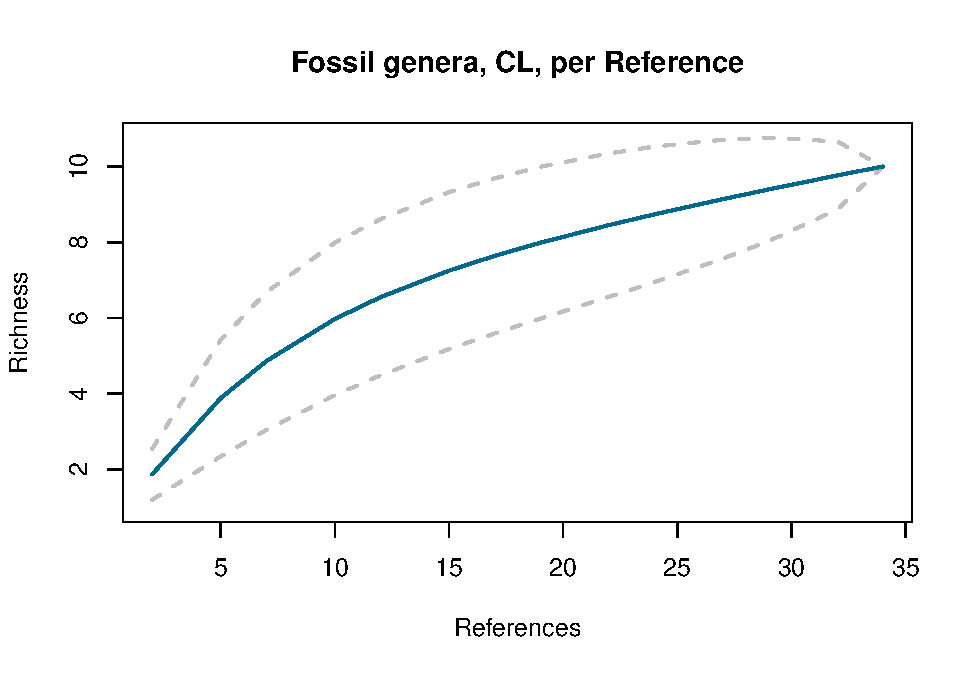
\includegraphics{MA_JJ_files/figure-latex/SACGAfrica-1.pdf}
\caption{Sampling Accumulation Curve of fossil genera per reference,
Africa}
\end{figure}

\begin{figure}[htbp]
\centering
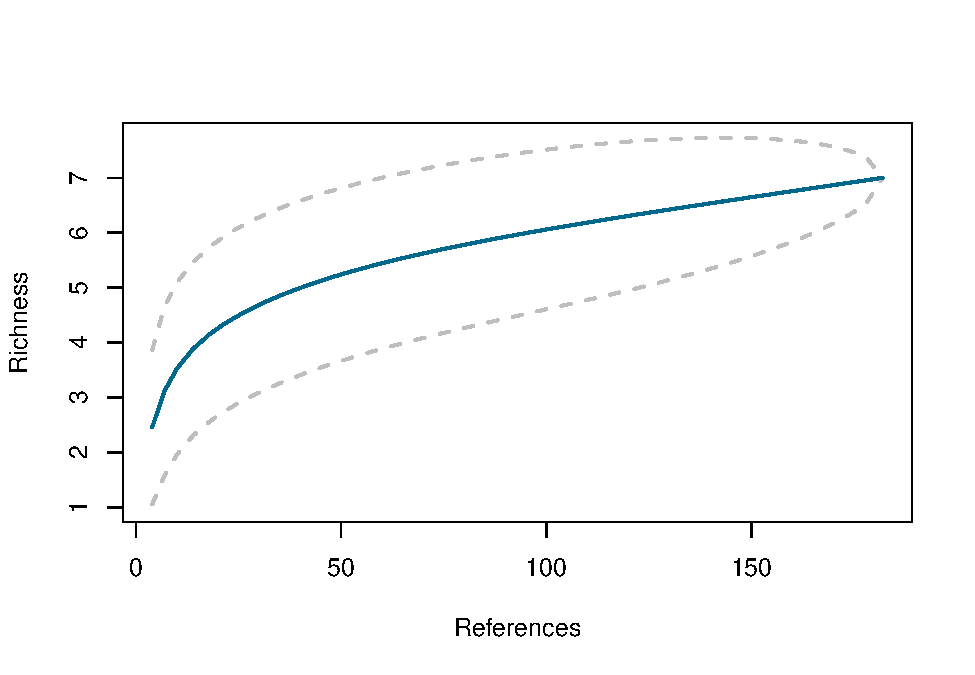
\includegraphics{MA_JJ_files/figure-latex/SACGAmerica-1.pdf}
\caption{Sampling Accumulation Curve of fossil genera per reference,
America}
\end{figure}

\begin{figure}[htbp]
\centering
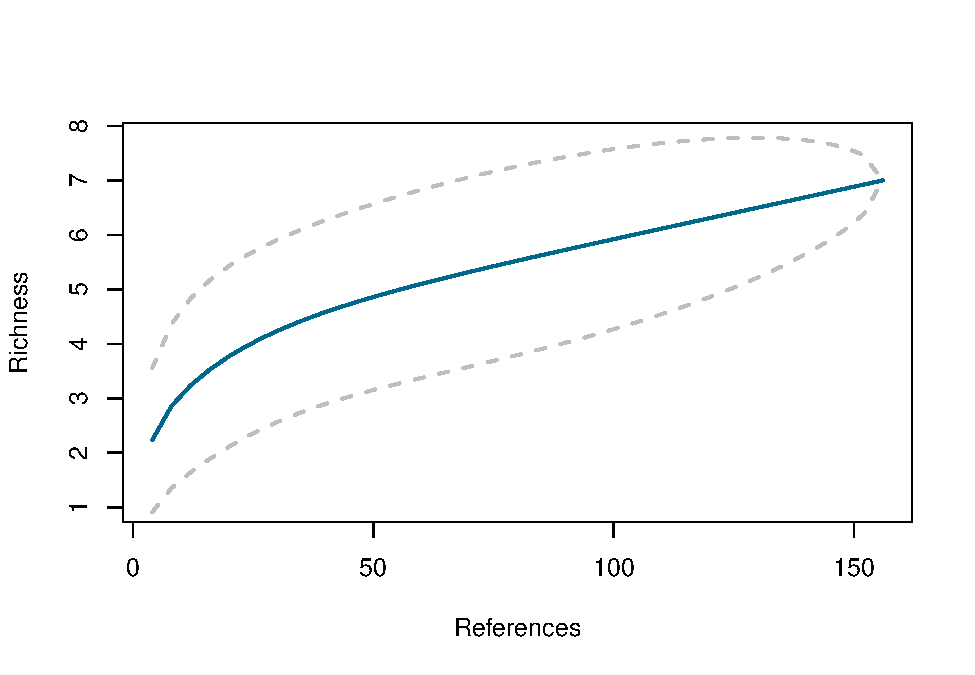
\includegraphics{MA_JJ_files/figure-latex/SACGNAmerica-1.pdf}
\caption{Sampling Accumulation Curve of fossil genera per reference,
N-America}
\end{figure}

\begin{figure}[htbp]
\centering
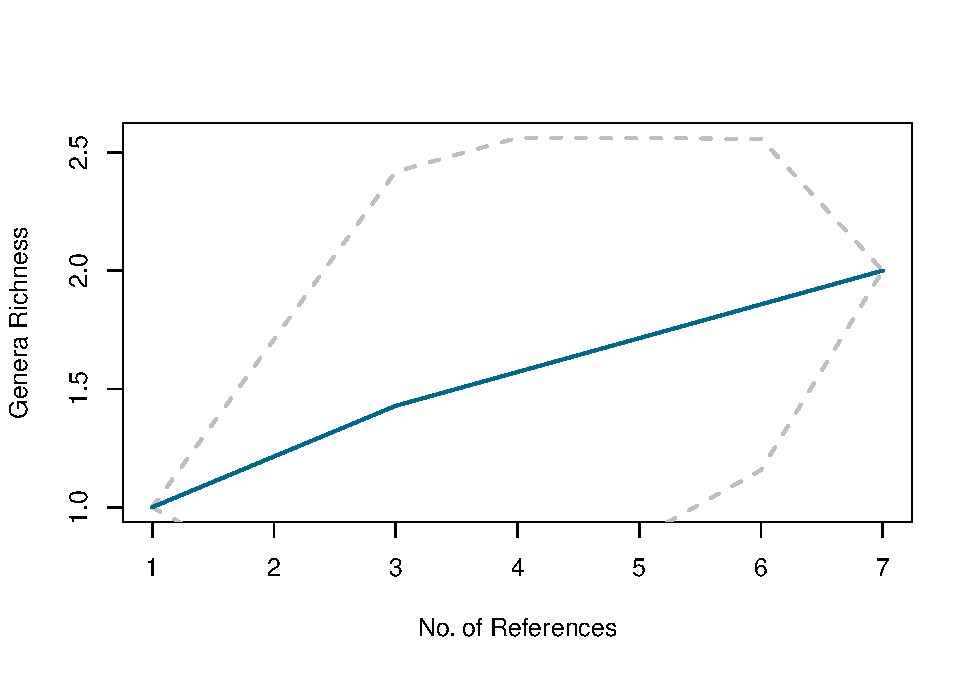
\includegraphics{MA_JJ_files/figure-latex/SACGSAmerica-1.pdf}
\caption{Sampling Accumulation Curve of fossil genera per reference,
S-America}
\end{figure}

\begin{figure}[htbp]
\centering
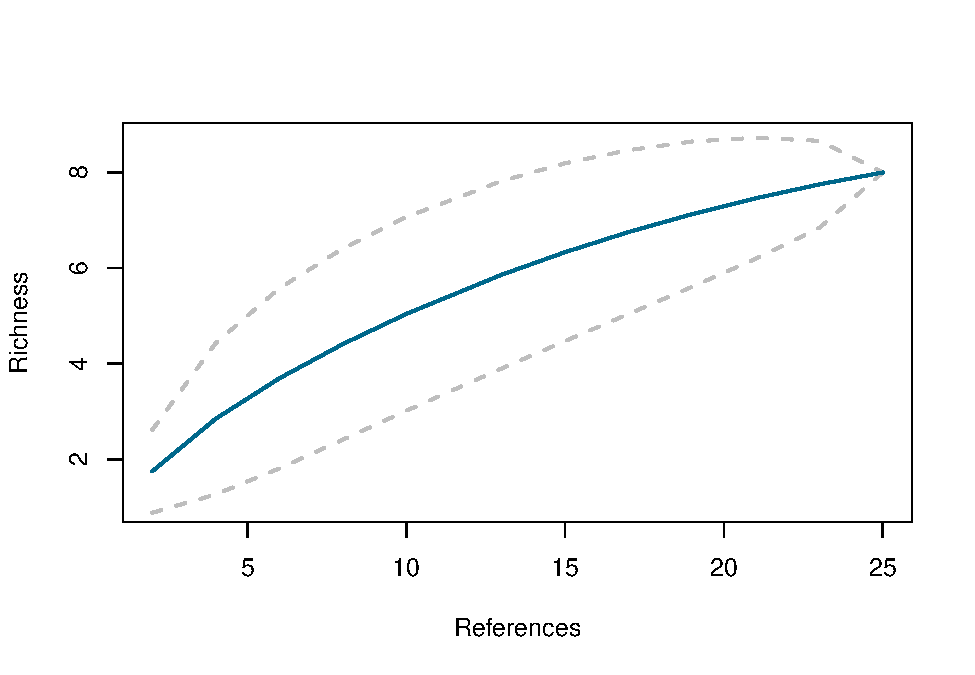
\includegraphics{MA_JJ_files/figure-latex/SACGAsia-1.pdf}
\caption{Sampling Accumulation Curve of fossil genera per reference,
Asia}
\end{figure}

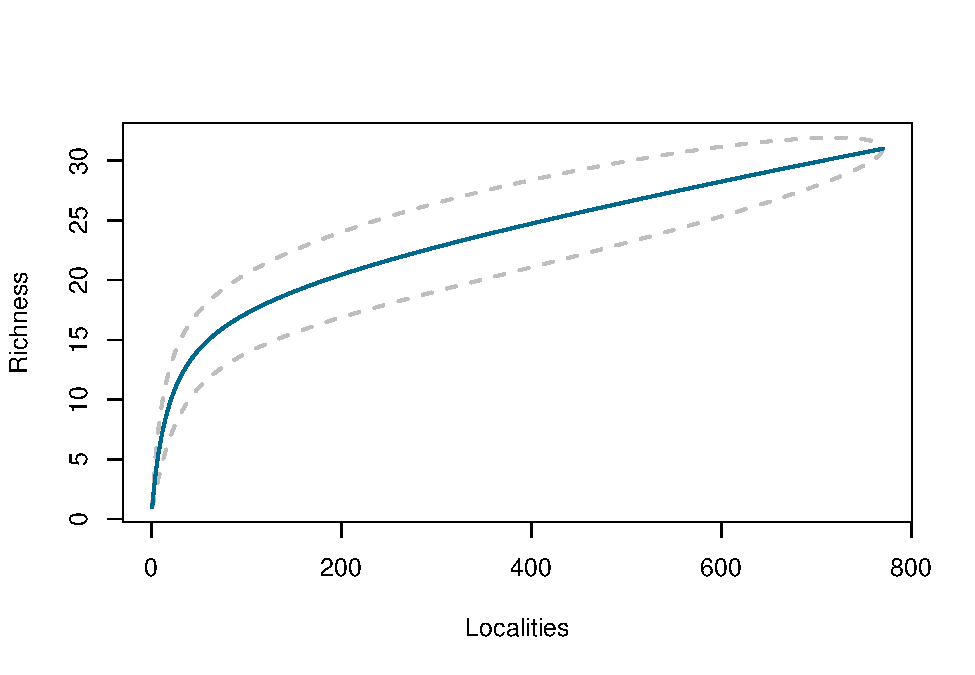
\includegraphics{MA_JJ_files/figure-latex/SAC fossil occurences-1.pdf}

\newpage

\section{Histograms}\label{histograms}

\subsection{all}\label{all}

\begin{verbatim}
## `stat_bin()` using `bins = 30`. Pick better value with `binwidth`.
\end{verbatim}

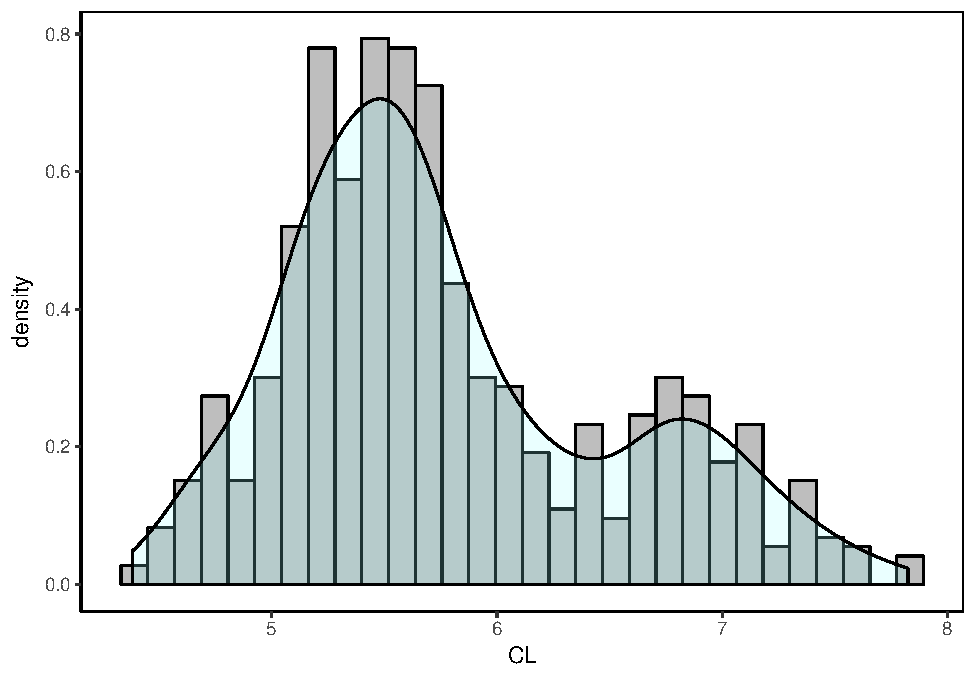
\includegraphics{MA_JJ_files/figure-latex/HistAll-1.pdf}
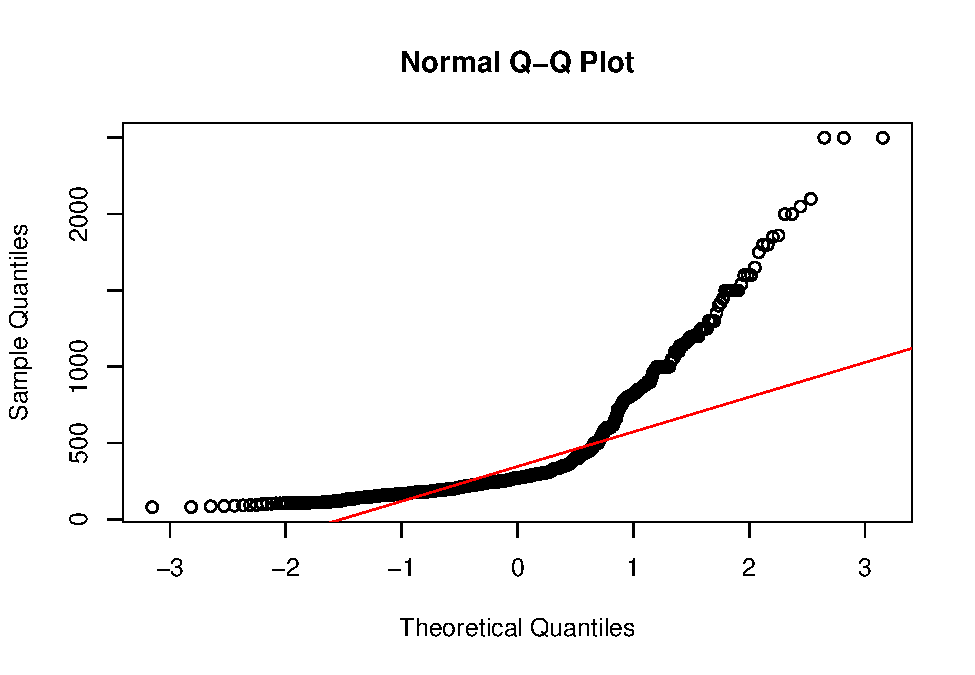
\includegraphics{MA_JJ_files/figure-latex/normalDistribution-1.pdf}
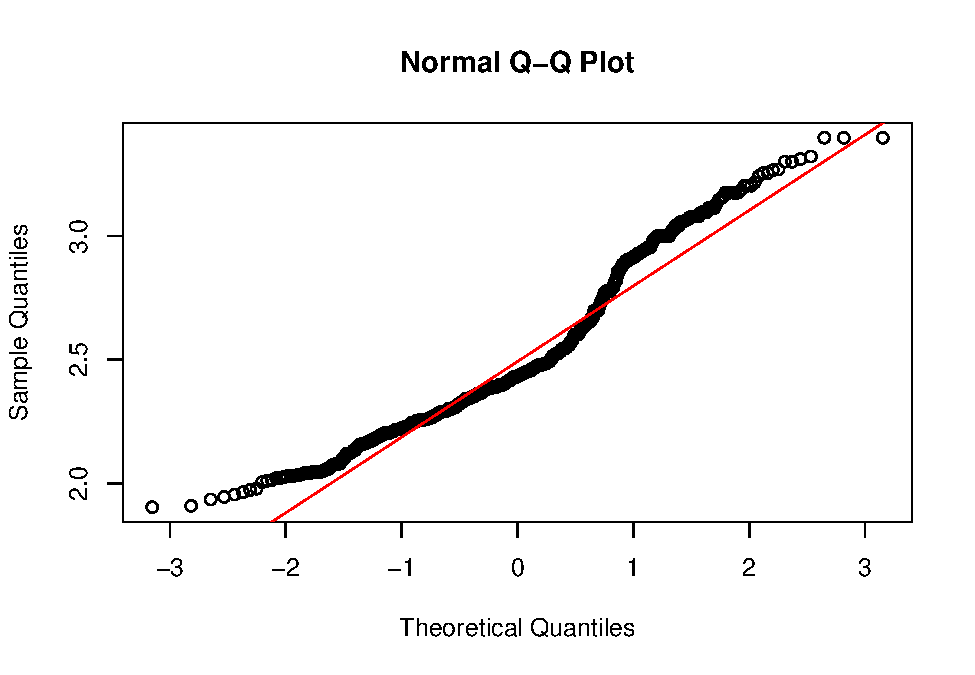
\includegraphics{MA_JJ_files/figure-latex/normalDistribution-2.pdf}

\newpage

\subsection{per time bin}\label{per-time-bin}

\begin{verbatim}
## `stat_bin()` using `bins = 30`. Pick better value with `binwidth`.
\end{verbatim}

\begin{figure}[htbp]
\centering
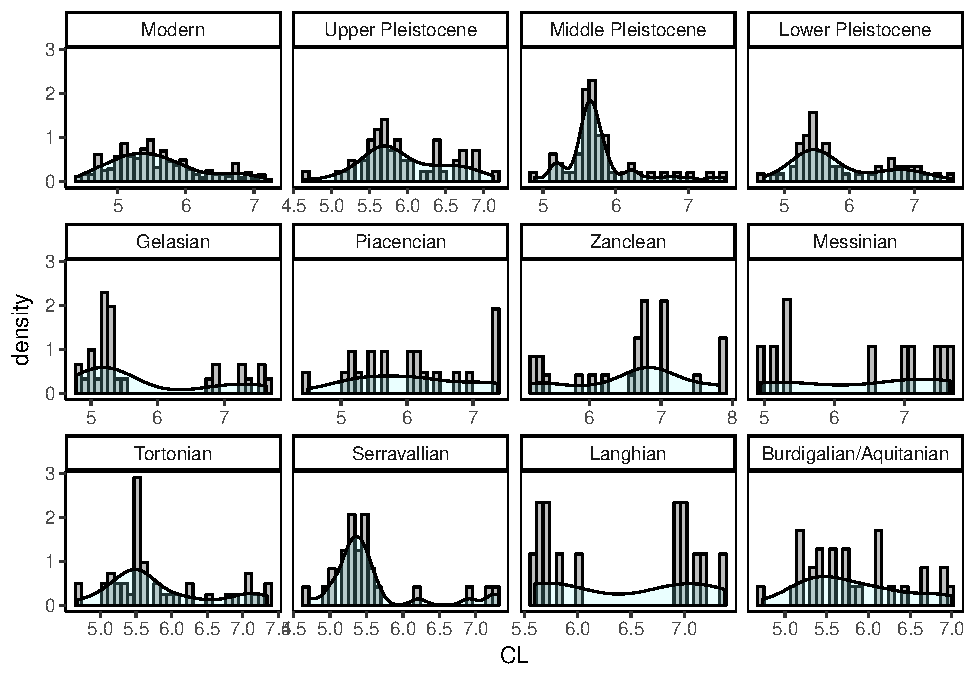
\includegraphics{MA_JJ_files/figure-latex/HistBins-1.pdf}
\caption{Distribution of body size data per time bin, logtransformed.}
\end{figure}

\newpage

\subsection{modern vs.~fossil}\label{modern-vs.fossil}

\begin{verbatim}
## `stat_bin()` using `bins = 30`. Pick better value with `binwidth`.
\end{verbatim}

\begin{figure}[htbp]
\centering
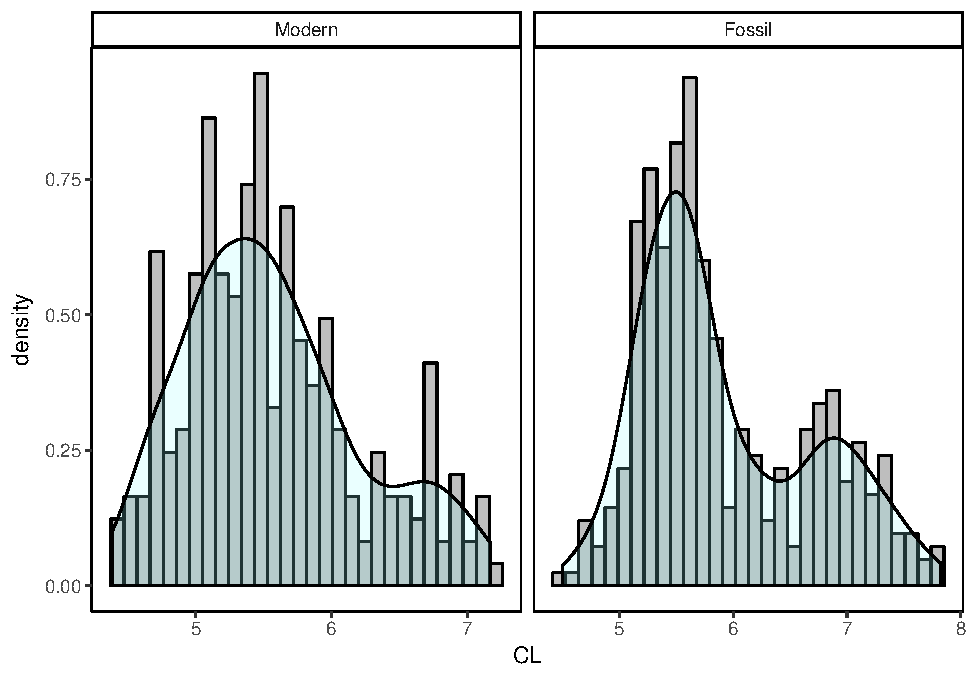
\includegraphics{MA_JJ_files/figure-latex/HistFosMo-1.pdf}
\caption{Distribution of body size data modern vs.~fossil,
logtransformed.}
\end{figure}

\newpage

\subsection{modern vs.~fossil, continental
vs.~insular}\label{modern-vs.fossil-continental-vs.insular}

\begin{verbatim}
## `stat_bin()` using `bins = 30`. Pick better value with `binwidth`.
\end{verbatim}

\begin{figure}[htbp]
\centering
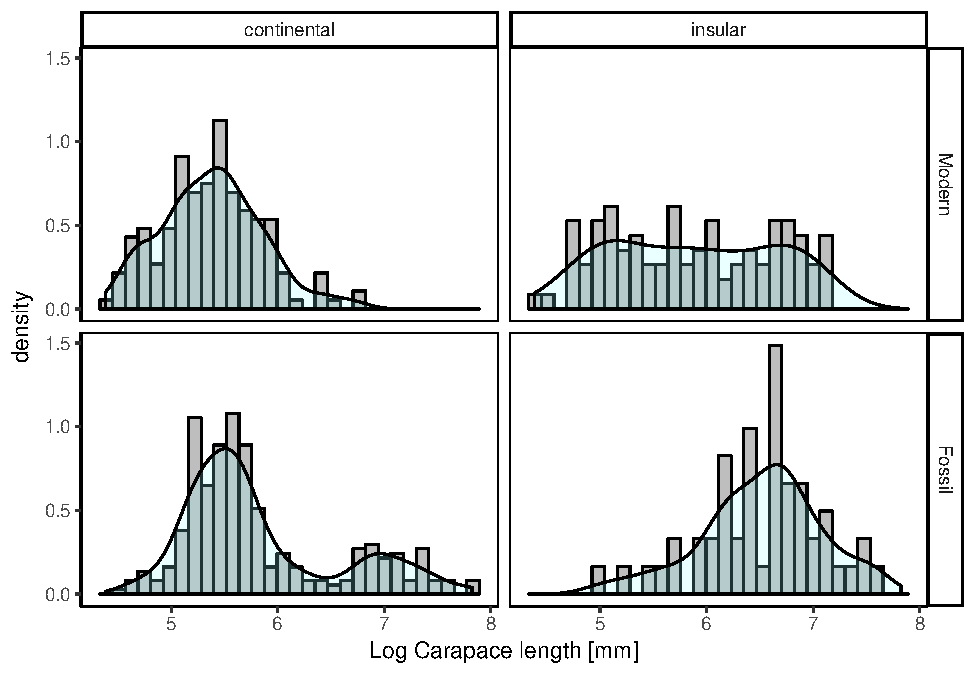
\includegraphics{MA_JJ_files/figure-latex/HistFMCI-1.pdf}
\caption{Distribution of body size data modern vs.~fossil, continental
vs.~insular logtransformed.}
\end{figure}

\newpage

\subsection{continental vs.~insular}\label{continental-vs.insular}

\begin{verbatim}
## `stat_bin()` using `bins = 30`. Pick better value with `binwidth`.
\end{verbatim}

\begin{figure}[htbp]
\centering
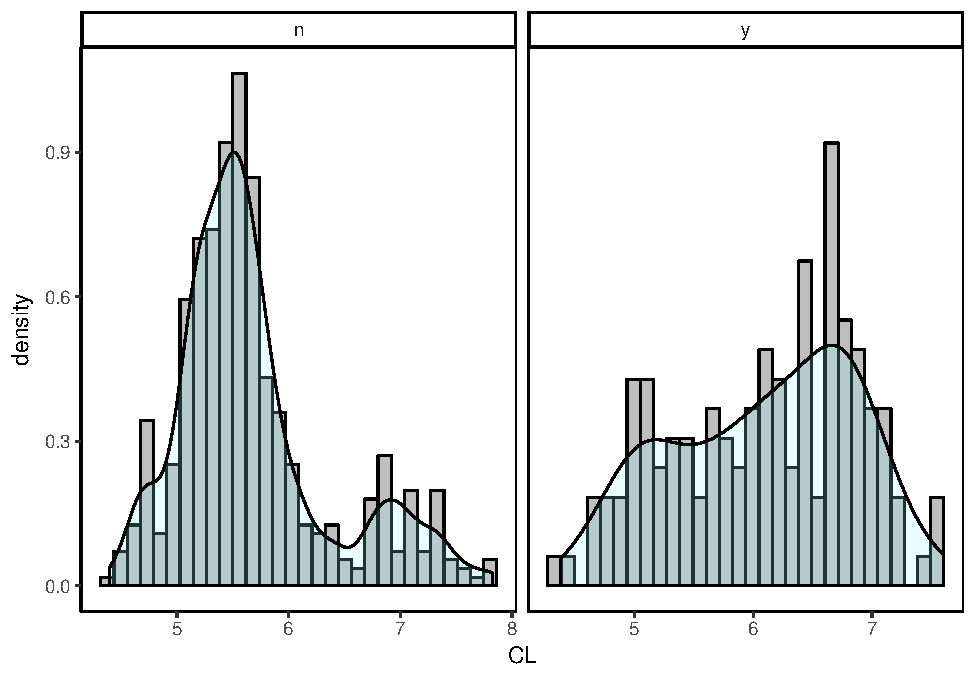
\includegraphics{MA_JJ_files/figure-latex/HistCI-1.pdf}
\caption{Distribution of body site data of continental (n) and
insular(y) species, logtransformed.}
\end{figure}

\newpage

\subsection{continents}\label{continents}

\begin{verbatim}
## `stat_bin()` using `bins = 30`. Pick better value with `binwidth`.
\end{verbatim}

\begin{figure}[htbp]
\centering
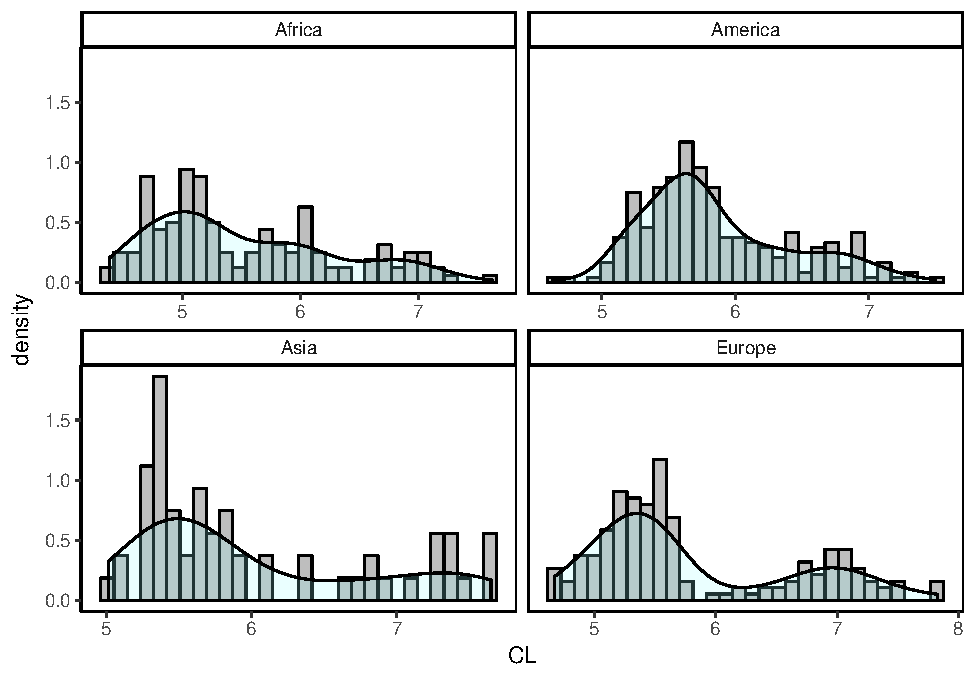
\includegraphics{MA_JJ_files/figure-latex/HistCon-1.pdf}
\caption{Distribution of body site data per continent, logtransformed.}
\end{figure}

\newpage

\subsection{Descriptive statistics}\label{descriptive-statistics}

\begin{longtable}[]{@{}rrrrrrrrrrrrl@{}}
\caption{General statistics of body size data: all, per time bin,
insular and continental, per continent (all referring to CL: min, max,
variance, mean, logmean, median, logmedian, skewness, logskewness,
kurosis, logkurtosis}\tabularnewline
\toprule
nCL & min & max & var & mean & logm & med & logmed & skew & logsk & kurt
& logku & Variable\tabularnewline
\midrule
\endfirsthead
\toprule
nCL & min & max & var & mean & logm & med & logmed & skew & logsk & kurt
& logku & Variable\tabularnewline
\midrule
\endhead
616 & 80.00 & 2500 & 164537.80 & 437.2 & 2.5 & 270.5 & 2.4 & 2.14 & 0.69
& 8.00 & 2.73 & all\tabularnewline
253 & 80.00 & 1300 & 67485.50 & 330.3 & 2.4 & 242.0 & 2.4 & 1.83 & 0.58
& 5.87 & 2.69 & Modern\tabularnewline
49 & 102.44 & 1250 & 69690.66 & 445.9 & 2.6 & 334.7 & 2.5 & 1.20 & 0.24
& 3.61 & 2.56 & Upper Pleistocene\tabularnewline
53 & 132.00 & 1800 & 97910.83 & 387.1 & 2.5 & 292.9 & 2.5 & 3.03 & 1.52
& 12.24 & 5.55 & Middle Pleistocene\tabularnewline
57 & 107.80 & 2000 & 161948.82 & 463.5 & 2.5 & 263.0 & 2.4 & 1.74 & 0.73
& 5.76 & 2.40 & Lower Pleistocene\tabularnewline
31 & 118.90 & 2050 & 411224.51 & 555.2 & 2.5 & 194.9 & 2.3 & 1.31 & 0.93
& 3.12 & 2.11 & Gelasian\tabularnewline
21 & 90.00 & 1600 & 270535.82 & 610.6 & 2.6 & 428.0 & 2.6 & 1.00 & 0.14
& 2.50 & 1.99 & Piacencian\tabularnewline
26 & 176.00 & 2500 & 476162.71 & 955.2 & 2.9 & 857.5 & 2.9 & 1.11 &
-0.40 & 3.56 & 2.30 & Zanclean\tabularnewline
10 & 140.00 & 2100 & 602611.21 & 948.9 & 2.8 & 916.0 & 2.9 & 0.26 &
-0.22 & 1.49 & 1.29 & Messinian\tabularnewline
45 & 107.00 & 1540 & 175470.12 & 462.7 & 2.5 & 250.0 & 2.4 & 1.49 & 0.81
& 3.74 & 2.54 & Tortonian\tabularnewline
27 & 111.00 & 1500 & 126060.40 & 337.7 & 2.4 & 220.0 & 2.3 & 2.49 & 1.77
& 7.77 & 5.30 & Serravallian\tabularnewline
14 & 270.00 & 1600 & 230451.33 & 747.9 & 2.8 & 700.0 & 2.8 & 0.30 & 0.03
& 1.55 & 1.18 & Langhian\tabularnewline
30 & 113.00 & 1100 & 76288.76 & 406.8 & 2.5 & 302.4 & 2.5 & 1.27 & 0.45
& 3.45 & 2.26 & Burdigalian/Aquitanian\tabularnewline
253 & 80.00 & 1300 & 67485.50 & 330.3 & 2.4 & 242.0 & 2.4 & 1.83 & 0.58
& 5.87 & 2.69 & Modern\tabularnewline
363 & 90.00 & 2500 & 219004.66 & 511.7 & 2.6 & 285.6 & 2.5 & 1.83 & 0.68
& 6.11 & 2.42 & Fossil\tabularnewline
469 & 81.00 & 2500 & 157808.79 & 392.9 & 2.5 & 250.0 & 2.4 & 2.65 & 1.07
& 10.57 & 3.74 & continental\tabularnewline
147 & 80.00 & 2000 & 160834.35 & 578.5 & 2.6 & 500.0 & 2.7 & 1.02 &
-0.27 & 3.95 & 2.05 & insular\tabularnewline
157 & 81.00 & 830 & 17009.02 & 244.0 & 2.3 & 221.0 & 2.3 & 1.92 & 0.29 &
8.09 & 2.98 & modern-con\tabularnewline
96 & 80.00 & 1300 & 118641.09 & 471.5 & 2.6 & 353.0 & 2.5 & 0.82 & 0.01
& 2.47 & 1.77 & modern-ins\tabularnewline
312 & 90.00 & 2500 & 212116.79 & 467.9 & 2.5 & 270.0 & 2.4 & 2.11 & 0.96
& 7.25 & 2.96 & fossil-con\tabularnewline
51 & 150.00 & 2000 & 180825.40 & 780.0 & 2.8 & 750.0 & 2.9 & 1.11 &
-0.40 & 4.02 & 3.18 & fossil-ins\tabularnewline
142 & 80.00 & 2050 & 112417.26 & 347.7 & 2.4 & 193.5 & 2.3 & 2.10 & 0.68
& 7.97 & 2.48 & Africa\tabularnewline
242 & 102.44 & 1800 & 82209.71 & 415.0 & 2.5 & 302.2 & 2.5 & 1.92 & 0.75
& 6.79 & 2.91 & America\tabularnewline
59 & 150.00 & 2100 & 323123.20 & 585.5 & 2.6 & 280.0 & 2.4 & 1.43 & 0.85
& 3.61 & 2.24 & Asia\tabularnewline
173 & 107.00 & 2500 & 254222.84 & 491.2 & 2.5 & 245.0 & 2.4 & 1.86 &
0.81 & 6.30 & 2.34 & Europe\tabularnewline
\bottomrule
\end{longtable}

\newpage

\section{Boxplots}\label{boxplots}

\subsection{genera per time bins}\label{genera-per-time-bins}

\begin{figure}[htbp]
\centering
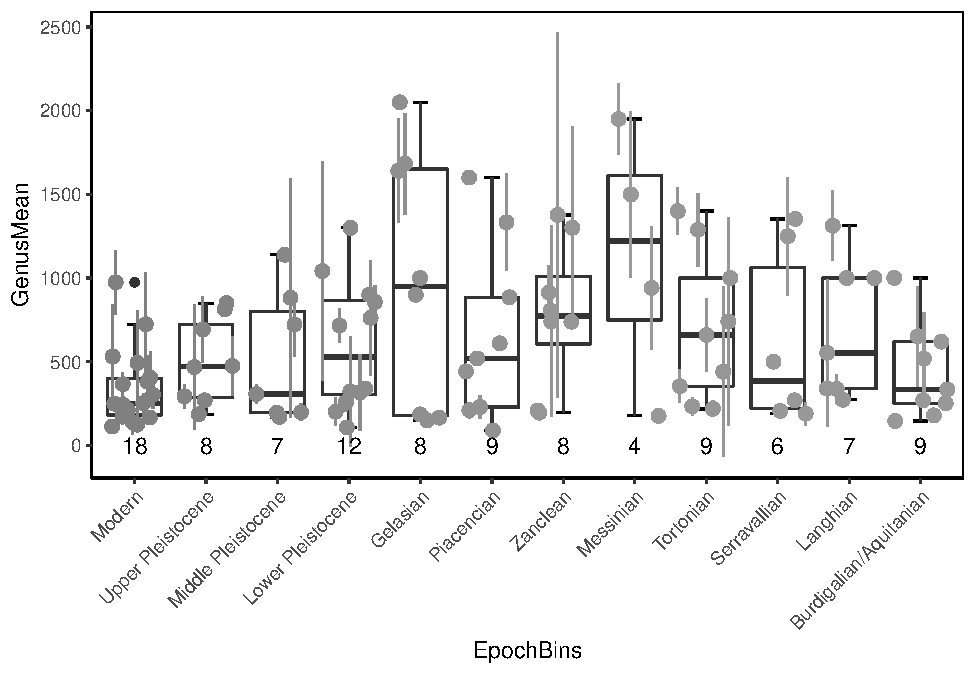
\includegraphics{MA_JJ_files/figure-latex/BPGBins-1.pdf}
\caption{Boxplots of mean CL per time bin, including mean and sd CL for
each genus (as pointrange).}
\end{figure}

\begin{verbatim}
## [1] "EpochBins" "Genus"     "GenusMean" "GenusSD"   "n"
\end{verbatim}

\begin{verbatim}
## Multiple comparison test after Kruskal-Wallis 
## p.value: 0.05 
## Comparisons
##                                              obs.dif critical.dif
## Modern-Upper Pleistocene                  16.7916667     43.58276
## Modern-Middle Pleistocene                 11.5238095     45.68715
## Modern-Lower Pleistocene                  20.7500000     38.22461
## Modern-Gelasian                           28.6666667     43.58276
## Modern-Piacencian                         21.0000000     41.87296
## Modern-Zanclean                           31.3541667     43.58276
## Modern-Messinian                          40.1666667     56.69626
## Modern-Tortonian                          28.2777778     41.87296
## Modern-Serravallian                       18.5000000     48.35073
## Modern-Langhian                           30.2380952     45.68715
## Modern-Burdigalian/Aquitanian              9.8888889     41.87296
## Upper Pleistocene-Middle Pleistocene       5.2678571     53.08367
## Upper Pleistocene-Lower Pleistocene        3.9583333     46.81540
## Upper Pleistocene-Gelasian                11.8750000     51.28370
## Upper Pleistocene-Piacencian               4.2083333     49.83880
## Upper Pleistocene-Zanclean                14.5625000     51.28370
## Upper Pleistocene-Messinian               23.3750000     62.80945
## Upper Pleistocene-Tortonian               11.4861111     49.83880
## Upper Pleistocene-Serravallian             1.7083333     55.39273
## Upper Pleistocene-Langhian                13.4464286     53.08367
## Upper Pleistocene-Burdigalian/Aquitanian   6.9027778     49.83880
## Middle Pleistocene-Lower Pleistocene       9.2261905     48.78053
## Middle Pleistocene-Gelasian               17.1428571     53.08367
## Middle Pleistocene-Piacencian              9.4761905     51.68911
## Middle Pleistocene-Zanclean               19.8303571     53.08367
## Middle Pleistocene-Messinian              28.6428571     64.28752
## Middle Pleistocene-Tortonian              16.7539683     51.68911
## Middle Pleistocene-Serravallian            6.9761905     57.06323
## Middle Pleistocene-Langhian               18.7142857     54.82458
## Middle Pleistocene-Burdigalian/Aquitanian  1.6349206     51.68911
## Lower Pleistocene-Gelasian                 7.9166667     46.81540
## Lower Pleistocene-Piacencian               0.2500000     45.22797
## Lower Pleistocene-Zanclean                10.6041667     46.81540
## Lower Pleistocene-Messinian               19.4166667     59.21731
## Lower Pleistocene-Tortonian                7.5277778     45.22797
## Lower Pleistocene-Serravallian             2.2500000     51.28370
## Lower Pleistocene-Langhian                 9.4880952     48.78053
## Lower Pleistocene-Burdigalian/Aquitanian  10.8611111     45.22797
## Gelasian-Piacencian                        7.6666667     49.83880
## Gelasian-Zanclean                          2.6875000     51.28370
## Gelasian-Messinian                        11.5000000     62.80945
## Gelasian-Tortonian                         0.3888889     49.83880
## Gelasian-Serravallian                     10.1666667     55.39273
## Gelasian-Langhian                          1.5714286     53.08367
## Gelasian-Burdigalian/Aquitanian           18.7777778     49.83880
## Piacencian-Zanclean                       10.3541667     49.83880
## Piacencian-Messinian                      19.1666667     61.63534
## Piacencian-Tortonian                       7.2777778     48.35073
## Piacencian-Serravallian                    2.5000000     54.05776
## Piacencian-Langhian                        9.2380952     51.68911
## Piacencian-Burdigalian/Aquitanian         11.1111111     48.35073
## Zanclean-Messinian                         8.8125000     62.80945
## Zanclean-Tortonian                         3.0763889     49.83880
## Zanclean-Serravallian                     12.8541667     55.39273
## Zanclean-Langhian                          1.1160714     53.08367
## Zanclean-Burdigalian/Aquitanian           21.4652778     49.83880
## Messinian-Tortonian                       11.8888889     61.63534
## Messinian-Serravallian                    21.6666667     66.20697
## Messinian-Langhian                         9.9285714     64.28752
## Messinian-Burdigalian/Aquitanian          30.2777778     61.63534
## Tortonian-Serravallian                     9.7777778     54.05776
## Tortonian-Langhian                         1.9603175     51.68911
## Tortonian-Burdigalian/Aquitanian          18.3888889     48.35073
## Serravallian-Langhian                     11.7380952     57.06323
## Serravallian-Burdigalian/Aquitanian        8.6111111     54.05776
## Langhian-Burdigalian/Aquitanian           20.3492063     51.68911
##                                           difference
## Modern-Upper Pleistocene                       FALSE
## Modern-Middle Pleistocene                      FALSE
## Modern-Lower Pleistocene                       FALSE
## Modern-Gelasian                                FALSE
## Modern-Piacencian                              FALSE
## Modern-Zanclean                                FALSE
## Modern-Messinian                               FALSE
## Modern-Tortonian                               FALSE
## Modern-Serravallian                            FALSE
## Modern-Langhian                                FALSE
## Modern-Burdigalian/Aquitanian                  FALSE
## Upper Pleistocene-Middle Pleistocene           FALSE
## Upper Pleistocene-Lower Pleistocene            FALSE
## Upper Pleistocene-Gelasian                     FALSE
## Upper Pleistocene-Piacencian                   FALSE
## Upper Pleistocene-Zanclean                     FALSE
## Upper Pleistocene-Messinian                    FALSE
## Upper Pleistocene-Tortonian                    FALSE
## Upper Pleistocene-Serravallian                 FALSE
## Upper Pleistocene-Langhian                     FALSE
## Upper Pleistocene-Burdigalian/Aquitanian       FALSE
## Middle Pleistocene-Lower Pleistocene           FALSE
## Middle Pleistocene-Gelasian                    FALSE
## Middle Pleistocene-Piacencian                  FALSE
## Middle Pleistocene-Zanclean                    FALSE
## Middle Pleistocene-Messinian                   FALSE
## Middle Pleistocene-Tortonian                   FALSE
## Middle Pleistocene-Serravallian                FALSE
## Middle Pleistocene-Langhian                    FALSE
## Middle Pleistocene-Burdigalian/Aquitanian      FALSE
## Lower Pleistocene-Gelasian                     FALSE
## Lower Pleistocene-Piacencian                   FALSE
## Lower Pleistocene-Zanclean                     FALSE
## Lower Pleistocene-Messinian                    FALSE
## Lower Pleistocene-Tortonian                    FALSE
## Lower Pleistocene-Serravallian                 FALSE
## Lower Pleistocene-Langhian                     FALSE
## Lower Pleistocene-Burdigalian/Aquitanian       FALSE
## Gelasian-Piacencian                            FALSE
## Gelasian-Zanclean                              FALSE
## Gelasian-Messinian                             FALSE
## Gelasian-Tortonian                             FALSE
## Gelasian-Serravallian                          FALSE
## Gelasian-Langhian                              FALSE
## Gelasian-Burdigalian/Aquitanian                FALSE
## Piacencian-Zanclean                            FALSE
## Piacencian-Messinian                           FALSE
## Piacencian-Tortonian                           FALSE
## Piacencian-Serravallian                        FALSE
## Piacencian-Langhian                            FALSE
## Piacencian-Burdigalian/Aquitanian              FALSE
## Zanclean-Messinian                             FALSE
## Zanclean-Tortonian                             FALSE
## Zanclean-Serravallian                          FALSE
## Zanclean-Langhian                              FALSE
## Zanclean-Burdigalian/Aquitanian                FALSE
## Messinian-Tortonian                            FALSE
## Messinian-Serravallian                         FALSE
## Messinian-Langhian                             FALSE
## Messinian-Burdigalian/Aquitanian               FALSE
## Tortonian-Serravallian                         FALSE
## Tortonian-Langhian                             FALSE
## Tortonian-Burdigalian/Aquitanian               FALSE
## Serravallian-Langhian                          FALSE
## Serravallian-Burdigalian/Aquitanian            FALSE
## Langhian-Burdigalian/Aquitanian                FALSE
\end{verbatim}

\begin{verbatim}
##  [1] "bin"          "Taxon"        "CL"           "extraCL"     
##  [5] "PL"           "size"         "estimated"    "Age"         
##  [9] "Island"       "Continent"    "Genus"        "EpochBins"   
## [13] "Stages"       "MeanBins"     "nIndividuals" "nSpecies"    
## [17] "nGenera"
\end{verbatim}

\begin{verbatim}
## Multiple comparison test after Kruskal-Wallis 
## p.value: 0.05 
## Comparisons
##                                              obs.dif critical.dif
## Modern-Upper Pleistocene                  116.987013     93.54915
## Modern-Middle Pleistocene                  80.140652     90.54349
## Modern-Lower Pleistocene                   66.123604     87.87753
## Modern-Gelasian                             1.627566    114.05459
## Modern-Piacencian                         113.296537    136.11314
## Modern-Zanclean                           205.945804    123.43828
## Modern-Messinian                          137.122727    193.24680
## Modern-Tortonian                           61.739394     96.96976
## Modern-Serravallian                        21.764310    121.34770
## Modern-Langhian                           202.487013    164.56067
## Modern-Burdigalian/Aquitanian              70.472727    115.73561
## Upper Pleistocene-Middle Pleistocene       36.846361    118.78423
## Upper Pleistocene-Lower Pleistocene        50.863409    116.76486
## Upper Pleistocene-Gelasian                115.359447    137.55006
## Upper Pleistocene-Piacencian                3.690476    156.32773
## Upper Pleistocene-Zanclean                 88.958791    145.42551
## Upper Pleistocene-Messinian                20.135714    207.98052
## Upper Pleistocene-Tortonian                55.247619    123.75260
## Upper Pleistocene-Serravallian            138.751323    143.65527
## Upper Pleistocene-Langhian                 85.500000    181.63641
## Upper Pleistocene-Burdigalian/Aquitanian   46.514286    138.94713
## Middle Pleistocene-Lower Pleistocene       14.017047    114.37094
## Middle Pleistocene-Gelasian                78.513086    135.52379
## Middle Pleistocene-Piacencian              33.155885    154.54785
## Middle Pleistocene-Zanclean               125.805152    143.51048
## Middle Pleistocene-Messinian               56.982075    206.64601
## Middle Pleistocene-Tortonian               18.401258    121.49644
## Middle Pleistocene-Serravallian           101.904962    141.71632
## Middle Pleistocene-Langhian               122.346361    180.10681
## Middle Pleistocene-Burdigalian/Aquitanian   9.667925    136.94153
## Lower Pleistocene-Gelasian                 64.496038    133.75738
## Lower Pleistocene-Piacencian               47.172932    153.00123
## Lower Pleistocene-Zanclean                139.822200    141.84356
## Lower Pleistocene-Messinian                70.999123    205.49188
## Lower Pleistocene-Tortonian                 4.384211    119.52289
## Lower Pleistocene-Serravallian             87.887914    140.02804
## Lower Pleistocene-Langhian                136.363409    178.78144
## Lower Pleistocene-Burdigalian/Aquitanian    4.349123    135.19364
## Gelasian-Piacencian                       111.668971    169.39706
## Gelasian-Zanclean                         204.318238    159.39129
## Gelasian-Messinian                        135.495161    217.97454
## Gelasian-Tortonian                         60.111828    139.89893
## Gelasian-Serravallian                      23.391876    157.77782
## Gelasian-Langhian                         200.859447    192.99946
## Gelasian-Burdigalian/Aquitanian            68.845161    153.50345
## Piacencian-Zanclean                        92.649267    175.85199
## Piacencian-Messinian                       23.826190    230.28513
## Piacencian-Tortonian                       51.557143    158.39839
## Piacencian-Serravallian                   135.060847    174.39088
## Piacencian-Langhian                        89.190476    206.80215
## Piacencian-Burdigalian/Aquitanian          42.823810    170.53342
## Zanclean-Messinian                         68.823077    223.02794
## Zanclean-Tortonian                        144.206410    147.64914
## Zanclean-Serravallian                     227.710114    164.68880
## Zanclean-Langhian                           3.458791    198.68908
## Zanclean-Burdigalian/Aquitanian           135.473077    160.59847
## Messinian-Tortonian                        75.383333    209.54137
## Messinian-Serravallian                    158.887037    221.87771
## Messinian-Langhian                         65.364286    248.16258
## Messinian-Burdigalian/Aquitanian           66.650000    218.85882
## Tortonian-Serravallian                     83.503704    145.90588
## Tortonian-Langhian                        140.747619    183.42158
## Tortonian-Burdigalian/Aquitanian            8.733333    141.27276
## Serravallian-Langhian                     224.251323    197.39708
## Serravallian-Burdigalian/Aquitanian        92.237037    158.99725
## Langhian-Burdigalian/Aquitanian           132.014286    193.99761
##                                           difference
## Modern-Upper Pleistocene                        TRUE
## Modern-Middle Pleistocene                      FALSE
## Modern-Lower Pleistocene                       FALSE
## Modern-Gelasian                                FALSE
## Modern-Piacencian                              FALSE
## Modern-Zanclean                                 TRUE
## Modern-Messinian                               FALSE
## Modern-Tortonian                               FALSE
## Modern-Serravallian                            FALSE
## Modern-Langhian                                 TRUE
## Modern-Burdigalian/Aquitanian                  FALSE
## Upper Pleistocene-Middle Pleistocene           FALSE
## Upper Pleistocene-Lower Pleistocene            FALSE
## Upper Pleistocene-Gelasian                     FALSE
## Upper Pleistocene-Piacencian                   FALSE
## Upper Pleistocene-Zanclean                     FALSE
## Upper Pleistocene-Messinian                    FALSE
## Upper Pleistocene-Tortonian                    FALSE
## Upper Pleistocene-Serravallian                 FALSE
## Upper Pleistocene-Langhian                     FALSE
## Upper Pleistocene-Burdigalian/Aquitanian       FALSE
## Middle Pleistocene-Lower Pleistocene           FALSE
## Middle Pleistocene-Gelasian                    FALSE
## Middle Pleistocene-Piacencian                  FALSE
## Middle Pleistocene-Zanclean                    FALSE
## Middle Pleistocene-Messinian                   FALSE
## Middle Pleistocene-Tortonian                   FALSE
## Middle Pleistocene-Serravallian                FALSE
## Middle Pleistocene-Langhian                    FALSE
## Middle Pleistocene-Burdigalian/Aquitanian      FALSE
## Lower Pleistocene-Gelasian                     FALSE
## Lower Pleistocene-Piacencian                   FALSE
## Lower Pleistocene-Zanclean                     FALSE
## Lower Pleistocene-Messinian                    FALSE
## Lower Pleistocene-Tortonian                    FALSE
## Lower Pleistocene-Serravallian                 FALSE
## Lower Pleistocene-Langhian                     FALSE
## Lower Pleistocene-Burdigalian/Aquitanian       FALSE
## Gelasian-Piacencian                            FALSE
## Gelasian-Zanclean                               TRUE
## Gelasian-Messinian                             FALSE
## Gelasian-Tortonian                             FALSE
## Gelasian-Serravallian                          FALSE
## Gelasian-Langhian                               TRUE
## Gelasian-Burdigalian/Aquitanian                FALSE
## Piacencian-Zanclean                            FALSE
## Piacencian-Messinian                           FALSE
## Piacencian-Tortonian                           FALSE
## Piacencian-Serravallian                        FALSE
## Piacencian-Langhian                            FALSE
## Piacencian-Burdigalian/Aquitanian              FALSE
## Zanclean-Messinian                             FALSE
## Zanclean-Tortonian                             FALSE
## Zanclean-Serravallian                           TRUE
## Zanclean-Langhian                              FALSE
## Zanclean-Burdigalian/Aquitanian                FALSE
## Messinian-Tortonian                            FALSE
## Messinian-Serravallian                         FALSE
## Messinian-Langhian                             FALSE
## Messinian-Burdigalian/Aquitanian               FALSE
## Tortonian-Serravallian                         FALSE
## Tortonian-Langhian                             FALSE
## Tortonian-Burdigalian/Aquitanian               FALSE
## Serravallian-Langhian                           TRUE
## Serravallian-Burdigalian/Aquitanian            FALSE
## Langhian-Burdigalian/Aquitanian                FALSE
\end{verbatim}

\begin{verbatim}
## 
##  Kruskal-Wallis rank sum test
## 
## data:  list(M, UPle, MPle, LPle, G, Pia, Z, Mess, Tort, S, L, BA)
## Kruskal-Wallis chi-squared = 71.441, df = 11, p-value = 6.496e-11
\end{verbatim}

\begin{verbatim}
## 
##  Wilcoxon rank sum test with continuity correction
## 
## data:  M and UPle
## W = 3853.5, p-value = 1.392e-05
## alternative hypothesis: true location shift is less than 0
\end{verbatim}

\begin{verbatim}
## [1] TRUE
\end{verbatim}

\begin{verbatim}
## 
##  Wilcoxon rank sum test with continuity correction
## 
## data:  UPle and MPle
## W = 1560, p-value = 0.08043
## alternative hypothesis: true location shift is not equal to 0
\end{verbatim}

\begin{verbatim}
## [1] FALSE
\end{verbatim}

\begin{verbatim}
## 
##  Wilcoxon rank sum test with continuity correction
## 
## data:  MPle and LPle
## W = 1643.5, p-value = 0.428
## alternative hypothesis: true location shift is not equal to 0
\end{verbatim}

\begin{verbatim}
## [1] FALSE
\end{verbatim}

\begin{verbatim}
## 
##  Wilcoxon rank sum test with continuity correction
## 
## data:  LPle and G
## W = 1124, p-value = 0.01802
## alternative hypothesis: true location shift is greater than 0
\end{verbatim}

\begin{verbatim}
## [1] TRUE
\end{verbatim}

\begin{verbatim}
## Warning in wilcox.test.default(G, Pia, paired = FALSE): cannot compute
## exact p-value with ties
\end{verbatim}

\begin{verbatim}
## 
##  Wilcoxon rank sum test with continuity correction
## 
## data:  G and Pia
## W = 246, p-value = 0.1406
## alternative hypothesis: true location shift is not equal to 0
\end{verbatim}

\begin{verbatim}
## [1] FALSE
\end{verbatim}

\begin{verbatim}
## Warning in wilcox.test.default(Pia, Z, paired = FALSE): cannot compute
## exact p-value with ties
\end{verbatim}

\begin{verbatim}
## 
##  Wilcoxon rank sum test with continuity correction
## 
## data:  Pia and Z
## W = 185.5, p-value = 0.06256
## alternative hypothesis: true location shift is not equal to 0
\end{verbatim}

\begin{verbatim}
## [1] FALSE
\end{verbatim}

\begin{verbatim}
## Warning in wilcox.test.default(Z, Mess, paired = FALSE): cannot compute
## exact p-value with ties
\end{verbatim}

\begin{verbatim}
## 
##  Wilcoxon rank sum test with continuity correction
## 
## data:  Z and Mess
## W = 134.5, p-value = 0.8876
## alternative hypothesis: true location shift is not equal to 0
\end{verbatim}

\begin{verbatim}
## [1] FALSE
\end{verbatim}

\begin{verbatim}
## Warning in wilcox.test.default(Mess, Tort, paired = FALSE): cannot compute
## exact p-value with ties
\end{verbatim}

\begin{verbatim}
## 
##  Wilcoxon rank sum test with continuity correction
## 
## data:  Mess and Tort
## W = 274.5, p-value = 0.2844
## alternative hypothesis: true location shift is not equal to 0
\end{verbatim}

\begin{verbatim}
## [1] FALSE
\end{verbatim}

\begin{verbatim}
## Warning in wilcox.test.default(Tort, S, paired = FALSE, alternative = "g"):
## cannot compute exact p-value with ties
\end{verbatim}

\begin{verbatim}
## 
##  Wilcoxon rank sum test with continuity correction
## 
## data:  Tort and S
## W = 810, p-value = 0.009363
## alternative hypothesis: true location shift is greater than 0
\end{verbatim}

\begin{verbatim}
## [1] TRUE
\end{verbatim}

\begin{verbatim}
## Warning in wilcox.test.default(S, L, paired = FALSE, alternative = "l"):
## cannot compute exact p-value with ties
\end{verbatim}

\begin{verbatim}
## 
##  Wilcoxon rank sum test with continuity correction
## 
## data:  S and L
## W = 45, p-value = 3.952e-05
## alternative hypothesis: true location shift is less than 0
\end{verbatim}

\begin{verbatim}
## [1] TRUE
\end{verbatim}

\begin{verbatim}
## Warning in wilcox.test.default(L, BA, paired = FALSE, alternative = "g"):
## cannot compute exact p-value with ties
\end{verbatim}

\begin{verbatim}
## 
##  Wilcoxon rank sum test with continuity correction
## 
## data:  L and BA
## W = 311, p-value = 0.005639
## alternative hypothesis: true location shift is greater than 0
\end{verbatim}

\begin{verbatim}
## [1] TRUE
\end{verbatim}

\begin{longtable}[]{@{}lrr@{}}
\toprule
lineage & pvalue & Bonferroni\tabularnewline
\midrule
\endhead
M and UPle & 0.0000139 & 0.0001531\tabularnewline
S and L & 0.0000395 & 0.0004347\tabularnewline
L and BA & 0.0056389 & 0.0620282\tabularnewline
Tort and S & 0.0093632 & 0.1029949\tabularnewline
LPle and G & 0.0180154 & 0.1981690\tabularnewline
Pia and Z & 0.0625644 & 0.6882088\tabularnewline
UPle and MPle & 0.0804319 & 0.8847504\tabularnewline
G and Pia & 0.1405871 & 1.0000000\tabularnewline
Mess and Tort & 0.2844360 & 1.0000000\tabularnewline
MPle and LPle & 0.4279860 & 1.0000000\tabularnewline
Z and Mess & 0.8876030 & 1.0000000\tabularnewline
\bottomrule
\end{longtable}

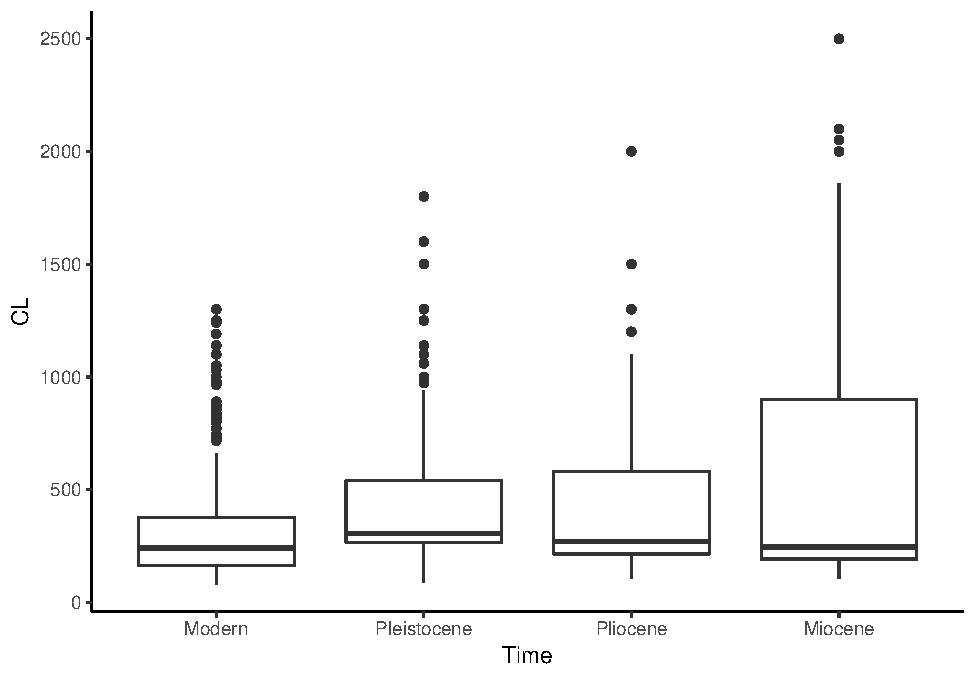
\includegraphics{MA_JJ_files/figure-latex/Boxplot Modern, Pleistocene etc.-1.pdf}
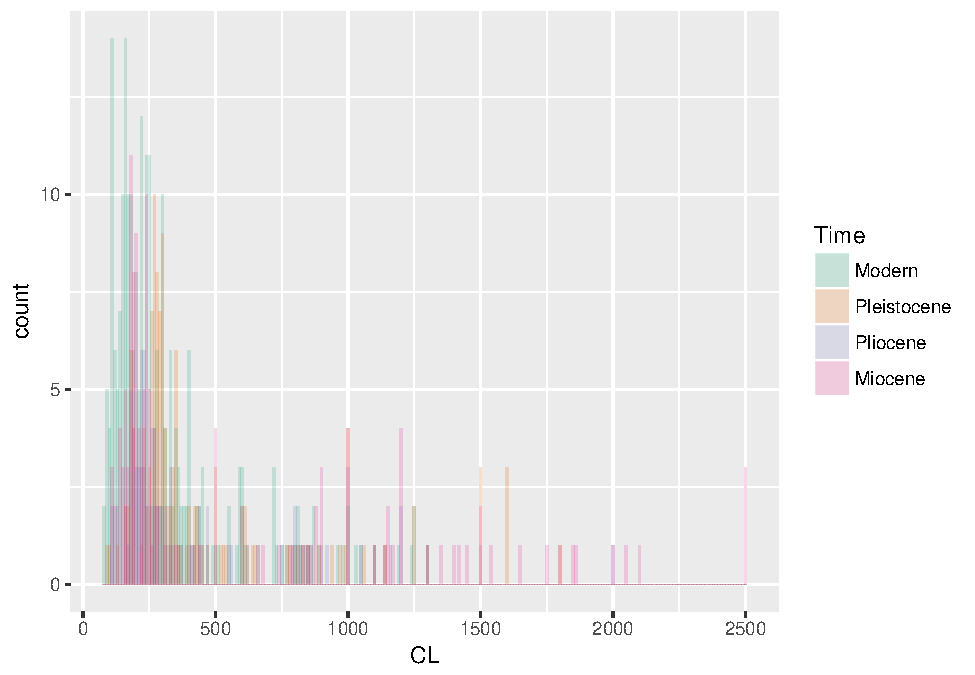
\includegraphics{MA_JJ_files/figure-latex/Boxplot Modern, Pleistocene etc.-2.pdf}

\begin{verbatim}
## 
##  Kruskal-Wallis rank sum test
## 
## data:  list(Modern, Plei, Plio, Mio)
## Kruskal-Wallis chi-squared = 37.764, df = 3, p-value = 3.172e-08
\end{verbatim}

\begin{verbatim}
##  [1] "EpochBins"    "bin"          "Taxon"        "CL"          
##  [5] "extraCL"      "PL"           "size"         "estimated"   
##  [9] "Age"          "Island"       "Continent"    "Genus"       
## [13] "Stages"       "MeanBins"     "nIndividuals" "nSpecies"    
## [17] "nGenera"      "Time"
\end{verbatim}

\begin{verbatim}
## Multiple comparison test after Kruskal-Wallis 
## p.value: 0.05 
## Comparisons
##                         obs.dif critical.dif difference
## Modern-Pleistocene   110.904114     49.80480       TRUE
## Modern-Pliocene       67.623302     58.35513       TRUE
## Modern-Miocene        64.510137     49.57182       TRUE
## Pleistocene-Pliocene  43.280812     64.36704      FALSE
## Pleistocene-Miocene   46.393977     56.52575      FALSE
## Pliocene-Miocene       3.113165     64.18694      FALSE
\end{verbatim}

\newpage

\subsection{continental vs.~insular per time
bin}\label{continental-vs.insular-per-time-bin}

\begin{figure}[htbp]
\centering
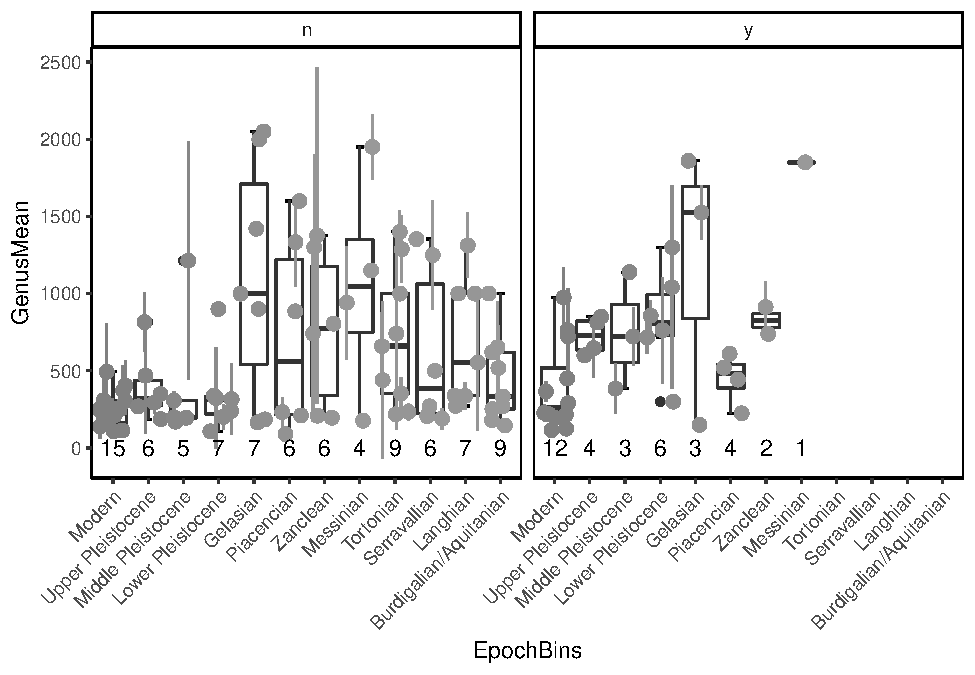
\includegraphics{MA_JJ_files/figure-latex/BPGBinsCI-1.pdf}
\caption{Boxplots of each genus per time bin, continental vs.~insular
species.}
\end{figure}

\newpage

\subsection{fossil vs.~modern}\label{fossil-vs.modern}

\begin{figure}[htbp]
\centering
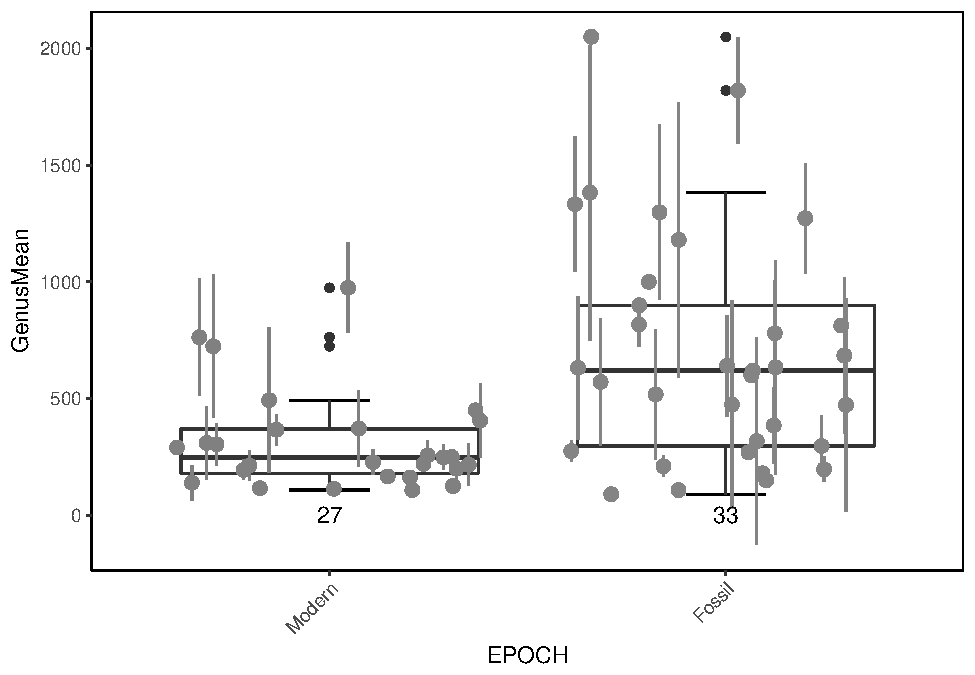
\includegraphics{MA_JJ_files/figure-latex/BPMF-1.pdf}
\caption{Boxplots fossil vs.~modern.}
\end{figure}

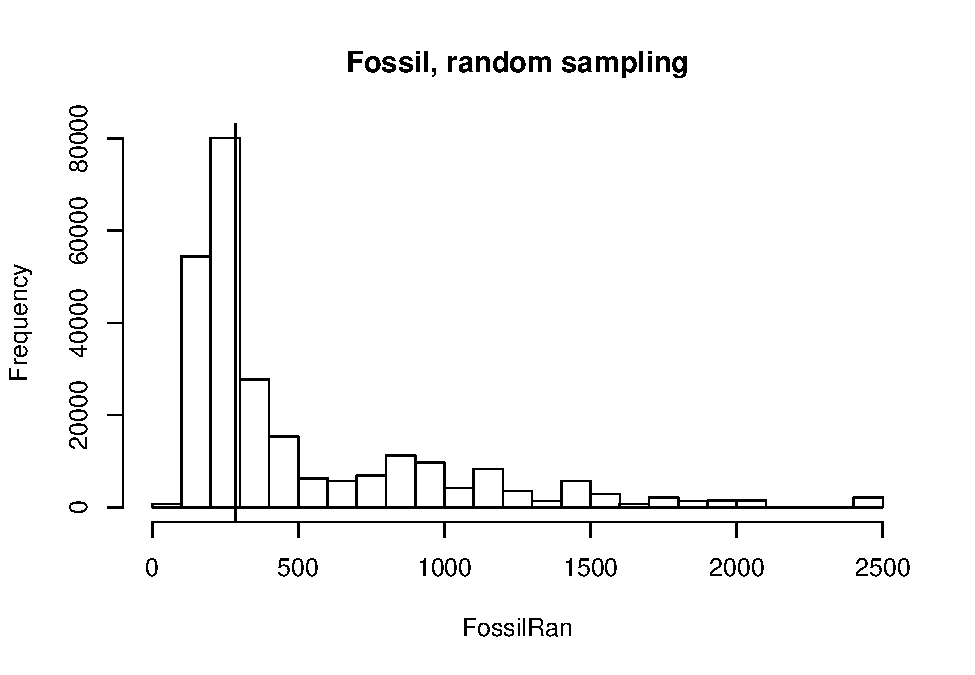
\includegraphics{MA_JJ_files/figure-latex/RSFM-1.pdf}

\begin{verbatim}
## [1] 330.3495
\end{verbatim}

\begin{verbatim}
## [1] 493.2024
\end{verbatim}

\begin{verbatim}
## 
##  Wilcoxon rank sum test with continuity correction
## 
## data:  Modern and Fossil
## W = 23910, p-value = 8.06e-07
## alternative hypothesis: true location shift is less than 0
\end{verbatim}

Wilcoxon Rank Sum Test (unpaired data):

modern \textless{} fossil (P = \(8.0601853\times 10^{-7}\))

\newpage

\subsection{fossil vs.~modern, continental
vs.~insular}\label{fossil-vs.modern-continental-vs.insular}

\begin{figure}[htbp]
\centering
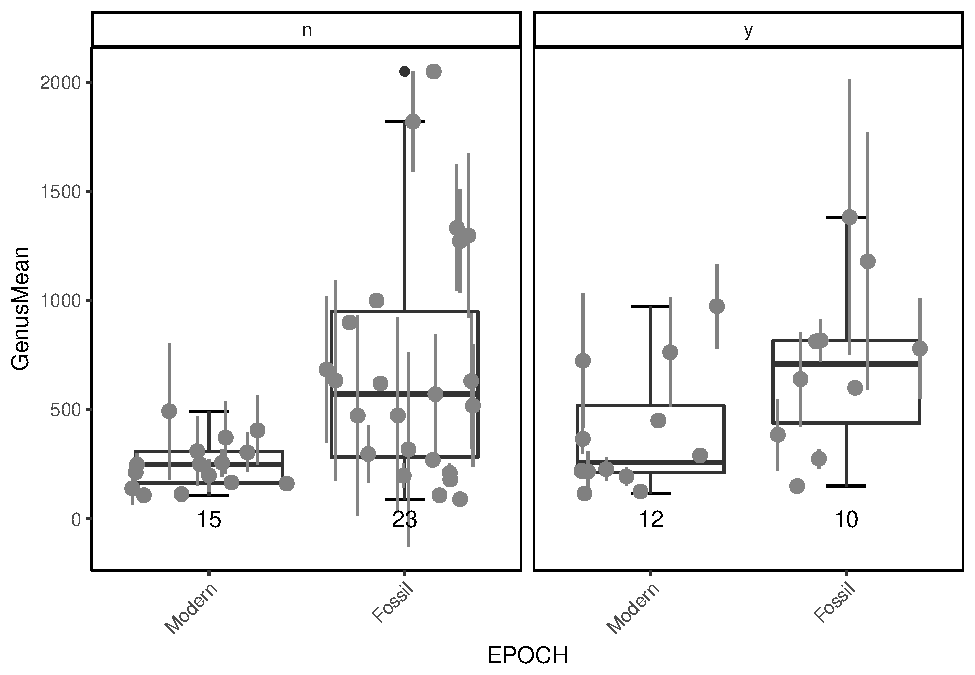
\includegraphics{MA_JJ_files/figure-latex/BPFMCI-1.pdf}
\caption{Boxplots fossil vs.~modern, continental vs.~insular species.}
\end{figure}

\begin{verbatim}
## [1] 51
\end{verbatim}

\begin{verbatim}
## [1] 51
\end{verbatim}

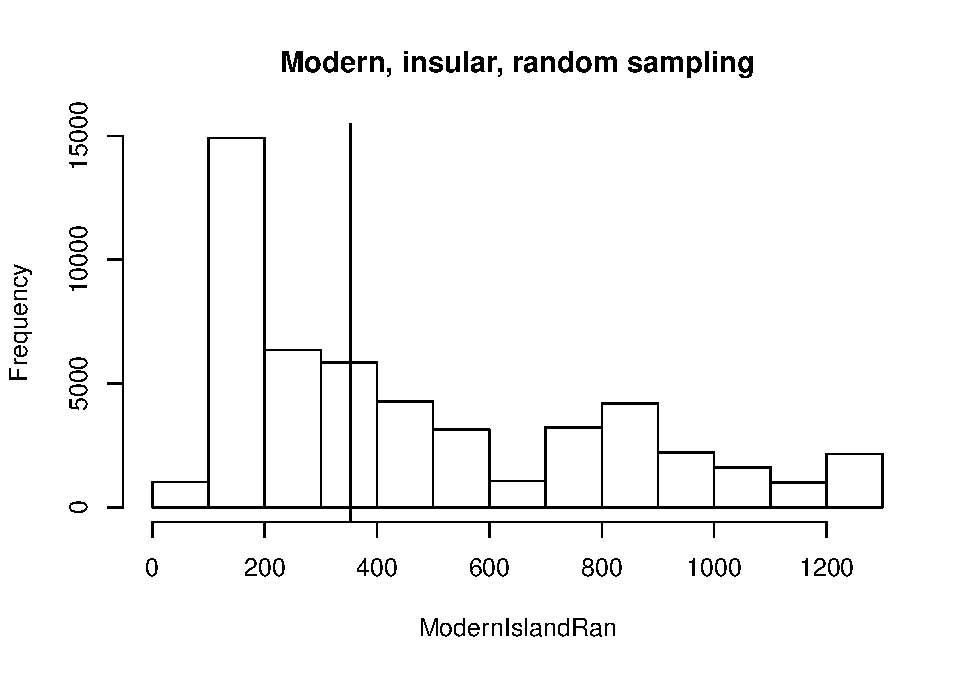
\includegraphics{MA_JJ_files/figure-latex/RSMFCI-1.pdf}

\begin{verbatim}
## 
##  Wilcoxon rank sum test with continuity correction
## 
## data:  ModernIsland and FossilIsland
## W = 736.5, p-value = 8.105e-05
## alternative hypothesis: true location shift is less than 0
\end{verbatim}

\begin{verbatim}
## [1] 157
\end{verbatim}

\begin{verbatim}
## [1] 157
\end{verbatim}

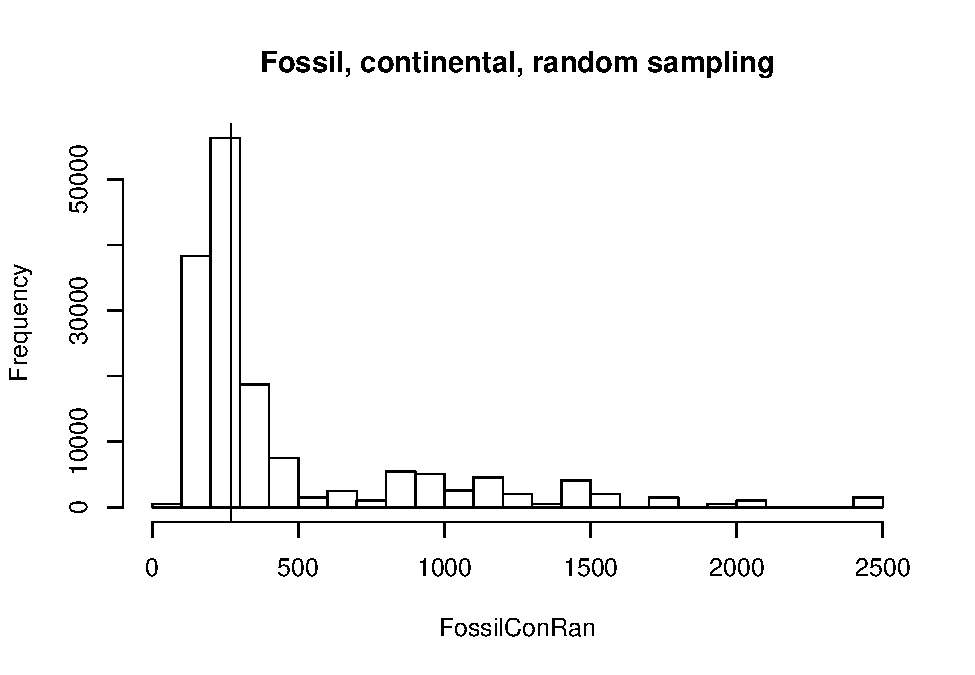
\includegraphics{MA_JJ_files/figure-latex/RSMFCI-2.pdf}

\begin{verbatim}
## 
##  Wilcoxon rank sum test with continuity correction
## 
## data:  ModernCon and FossilCon
## W = 8618.5, p-value = 2.045e-06
## alternative hypothesis: true location shift is less than 0
\end{verbatim}

Wilcoxon Rank Sum Test (unpaired data):

modern continental \textless{} fossil continental (P =
\(2.0453428\times 10^{-6}\))

modern insular \textless{} fossil insular (P =
\(8.1054671\times 10^{-5}\))

\newpage

\subsection{continental vs.~insular}\label{continental-vs.insular-1}

\begin{figure}[htbp]
\centering
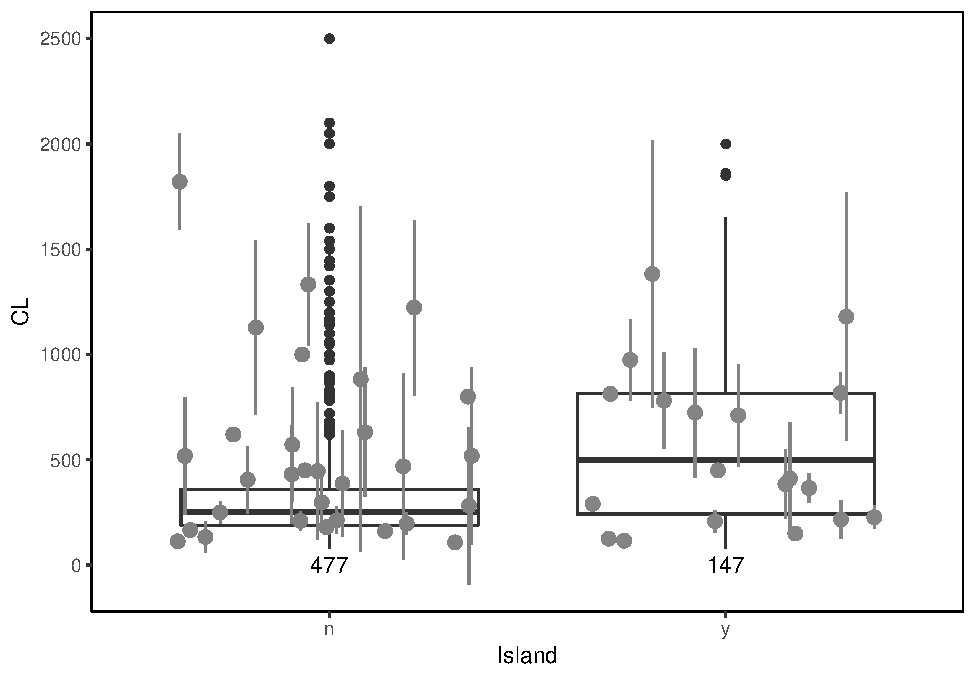
\includegraphics{MA_JJ_files/figure-latex/BPCI-1.pdf}
\caption{Boxplot continental vs.~insular, genera summarised}
\end{figure}

\begin{verbatim}
## [1] 147
\end{verbatim}

\begin{verbatim}
## [1] 147
\end{verbatim}

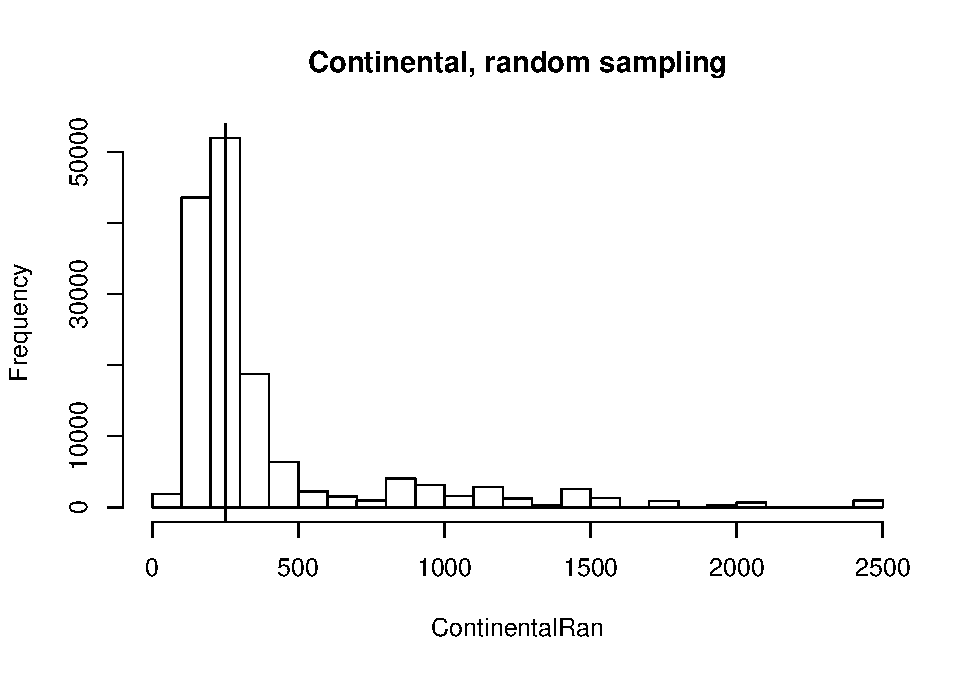
\includegraphics{MA_JJ_files/figure-latex/RSCI-1.pdf}

\begin{verbatim}
## 
##  Wilcoxon rank sum test with continuity correction
## 
## data:  Insular and Continental
## W = 14486, p-value = 2.21e-07
## alternative hypothesis: true location shift is greater than 0
\end{verbatim}

Wilcoxon Rank Sum Test (unpaired data):

continental \textless{} insular (P = \(2.2103293\times 10^{-7}\))

\newpage

\subsection{continental vs.~insular per time
bin}\label{continental-vs.insular-per-time-bin-1}

\begin{figure}[htbp]
\centering
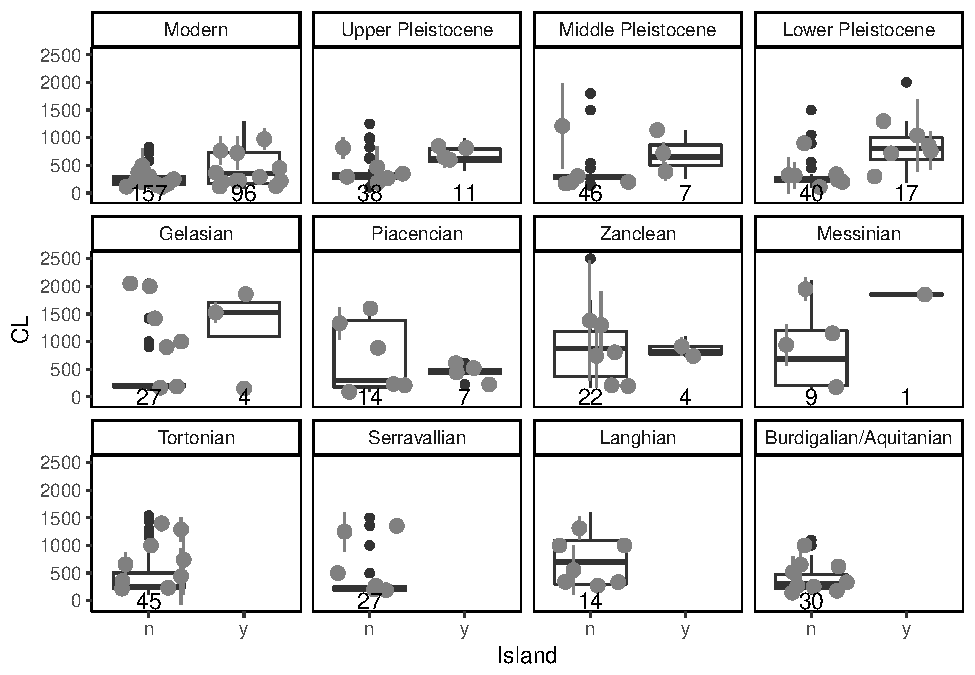
\includegraphics{MA_JJ_files/figure-latex/BPCIBins-1.pdf}
\caption{Boxplot continental vs.~insular, genera summarised}
\end{figure}

\newpage

\subsection{continents}\label{continents-1}

\begin{figure}[htbp]
\centering
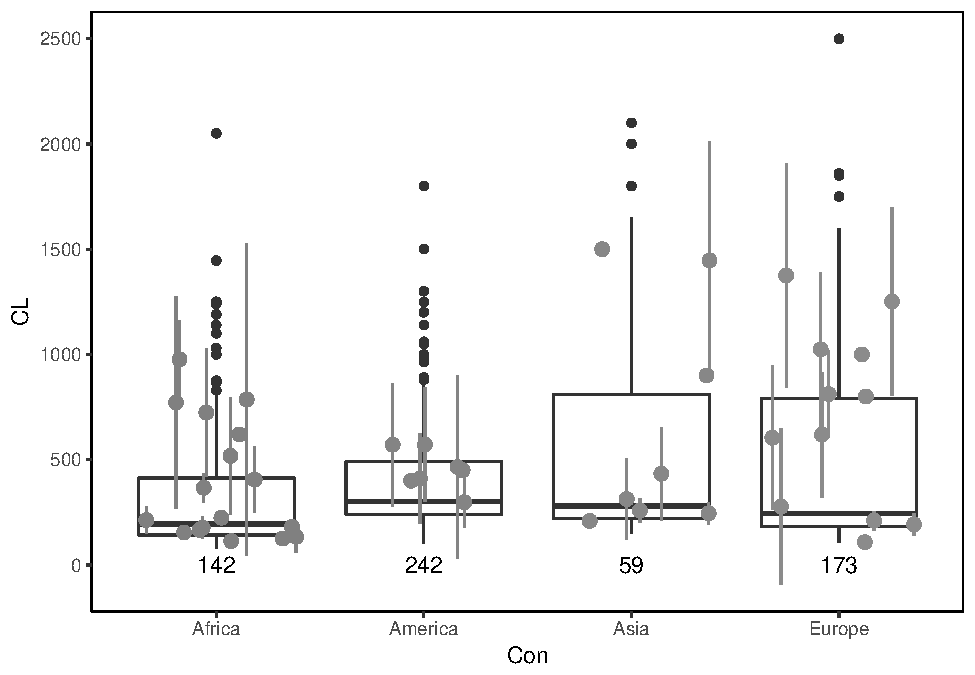
\includegraphics{MA_JJ_files/figure-latex/BPCon-1.pdf}
\caption{Boxplot: body size on different continents, genera summarised}
\end{figure}

\begin{verbatim}
##  [1] "Continent"    "bin"          "Taxon"        "CL"          
##  [5] "extraCL"      "PL"           "size"         "estimated"   
##  [9] "Age"          "Island"       "Genus"        "EpochBins"   
## [13] "Stages"       "MeanBins"     "nIndividuals" "nSpecies"    
## [17] "nGenera"      "Con"
\end{verbatim}

\begin{table}

\centering
\begin{tabular}[t]{l}
\hline
Multiple comparison test after Kruskal-Wallis\\
\hline
\end{tabular}
\centering
\begin{tabular}[t]{r}
\hline
0.05\\
\hline
\end{tabular}
\centering
\begin{tabular}[t]{l|r|r|l}
\hline
  & obs.dif & critical.dif & difference\\
\hline
Africa-America & 108.957339 & 49.63331 & TRUE\\
\hline
Africa-Asia & 118.618286 & 72.72560 & TRUE\\
\hline
Africa-Europe & 58.612310 & 53.16766 & TRUE\\
\hline
America-Asia & 9.660947 & 68.17247 & FALSE\\
\hline
America-Europe & 50.345029 & 46.74690 & TRUE\\
\hline
Asia-Europe & 60.005976 & 70.78714 & FALSE\\
\hline
\end{tabular}
\end{table}

\begin{verbatim}
## [1] 142
\end{verbatim}

\begin{verbatim}
## [1] 347.6887
\end{verbatim}

\begin{verbatim}
## [1] 142
\end{verbatim}

\begin{verbatim}
## [1] 427.6447
\end{verbatim}

\begin{verbatim}
## [1] 59
\end{verbatim}

\begin{verbatim}
## [1] 173
\end{verbatim}

\begin{verbatim}
## [1] 142
\end{verbatim}

\begin{verbatim}
## [1] 530.7401
\end{verbatim}

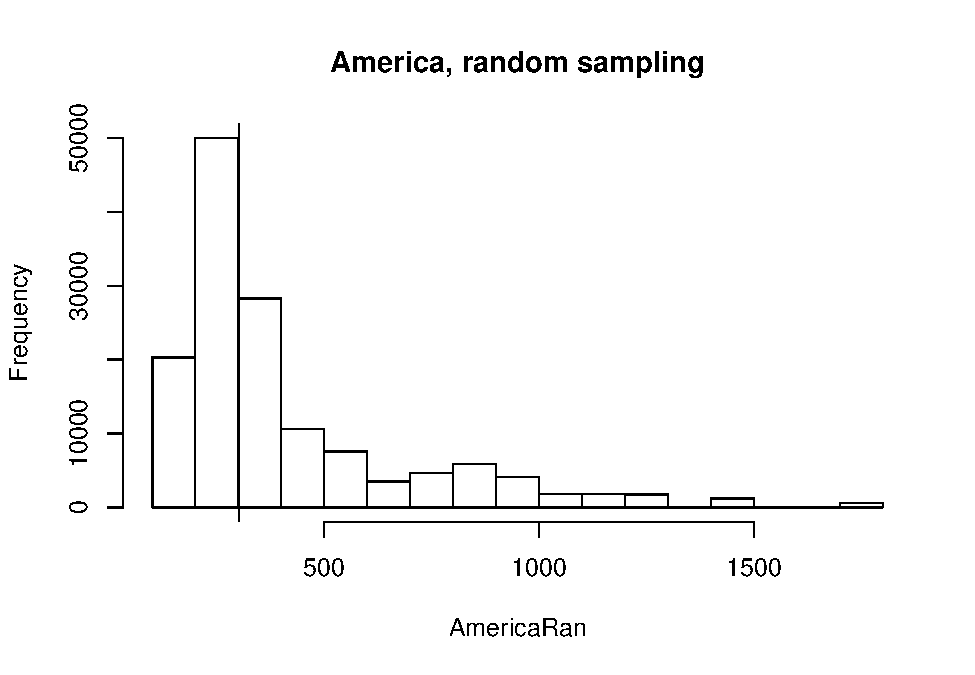
\includegraphics{MA_JJ_files/figure-latex/RSCon-1.pdf}
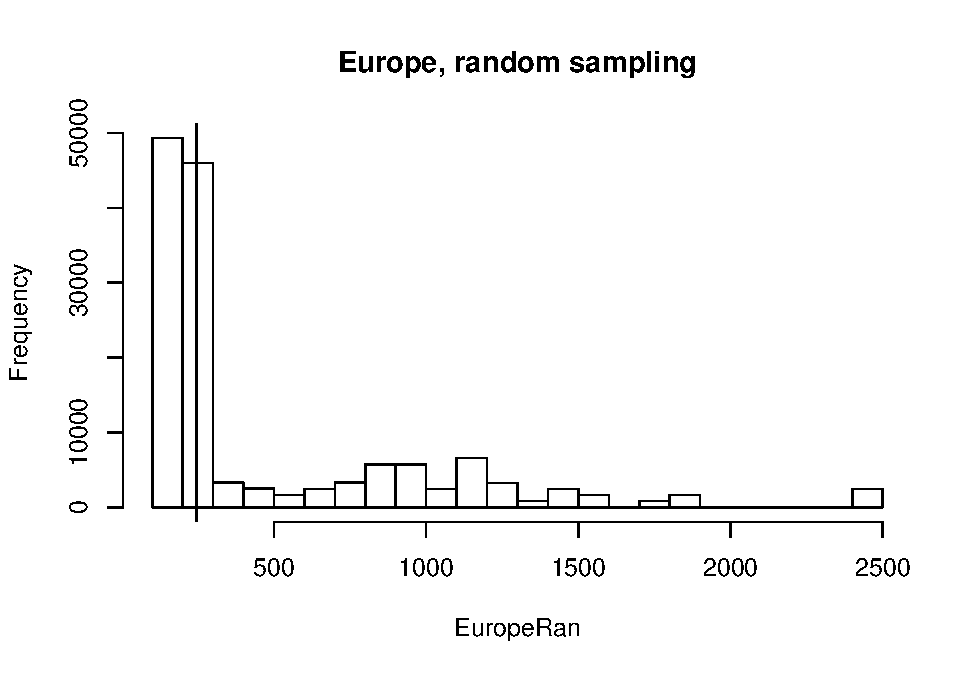
\includegraphics{MA_JJ_files/figure-latex/RSCon-2.pdf}
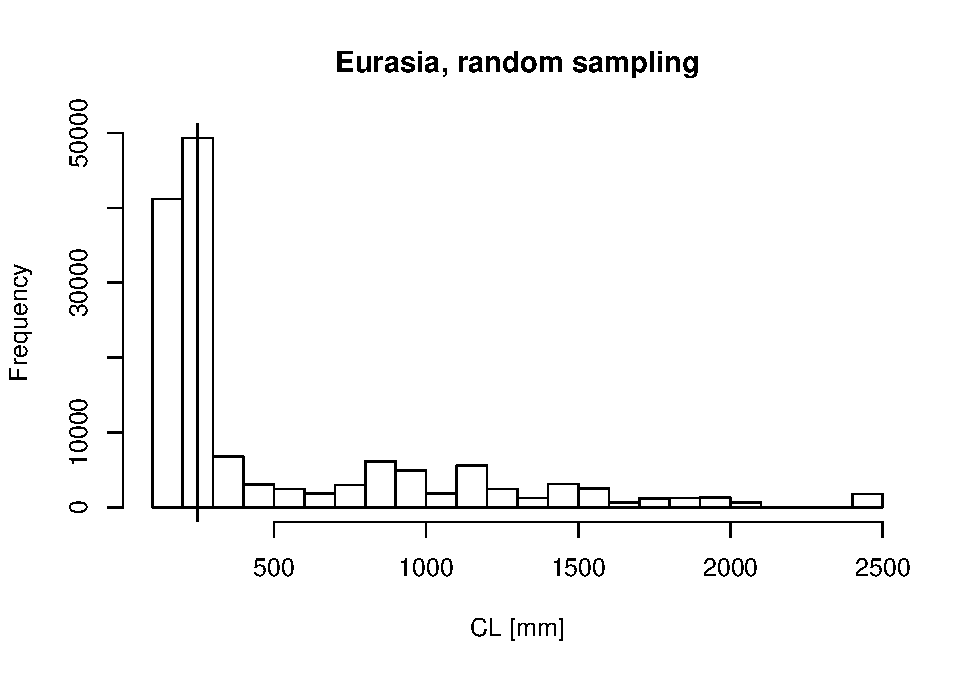
\includegraphics{MA_JJ_files/figure-latex/RSCon-3.pdf}

\begin{verbatim}
## 
##  Kruskal-Wallis rank sum test
## 
## data:  list(Africa, America, Eurasia, Europe)
## Kruskal-Wallis chi-squared = 36.614, df = 3, p-value = 5.554e-08
\end{verbatim}

Kruskal-Wallis-Test:

Continent means differ (P = \(5.5537507\times 10^{-8}\)) (still have to
look into the details\ldots{})

\newpage

\subsection{continents, continental
vs.~insular}\label{continents-continental-vs.insular}

\begin{figure}[htbp]
\centering
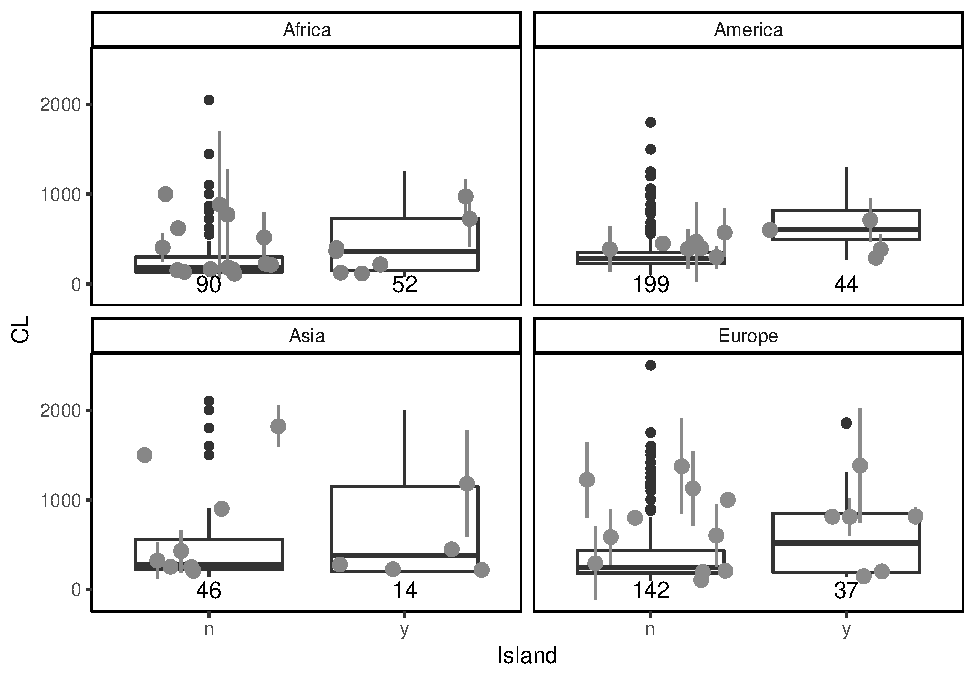
\includegraphics{MA_JJ_files/figure-latex/BPConCI-1.pdf}
\caption{Boxplot: body size on different continents, genera summarised}
\end{figure}

\newpage

\section{paleoTS analysis}\label{paleots-analysis}

\subsection{all (continental and
insular)}\label{all-continental-and-insular}

\subsubsection{genera (all)}\label{genera-all}

\begin{longtable}[]{@{}rrrr@{}}
\caption{paleoTS object, all data}\tabularnewline
\toprule
tt & nn & mm & vv\tabularnewline
\midrule
\endfirsthead
\toprule
tt & nn & mm & vv\tabularnewline
\midrule
\endhead
0.00585 & 22 & 330.1456 & 50307.87\tabularnewline
0.06885 & 8 & 506.3265 & 64620.11\tabularnewline
0.45350 & 7 & 516.4053 & 155241.85\tabularnewline
1.29350 & 12 & 593.8669 & 147507.20\tabularnewline
2.19700 & 8 & 971.8850 & 580540.76\tabularnewline
3.09400 & 9 & 658.0826 & 271043.73\tabularnewline
4.46600 & 8 & 785.0792 & 187937.61\tabularnewline
6.28900 & 4 & 1141.9375 & 584378.85\tabularnewline
9.42700 & 9 & 703.9570 & 195766.19\tabularnewline
12.71400 & 6 & 628.3020 & 285258.36\tabularnewline
14.89500 & 7 & 687.9619 & 169914.58\tabularnewline
19.50000 & 9 & 441.5420 & 78467.65\tabularnewline
\bottomrule
\end{longtable}

\begin{figure}[htbp]
\centering
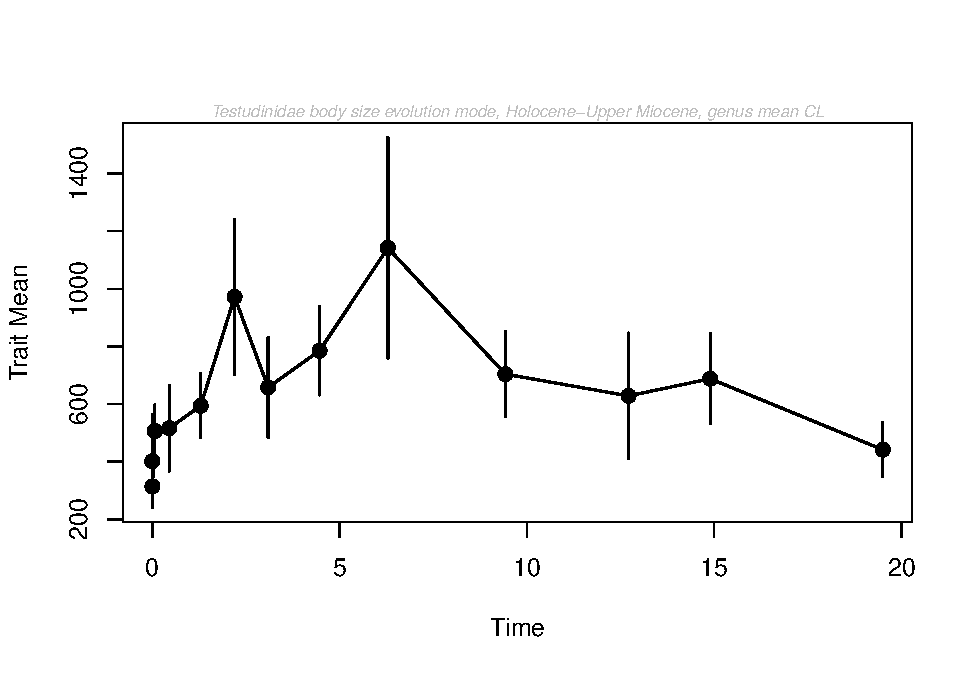
\includegraphics{MA_JJ_files/figure-latex/paleoTSAll-1.pdf}
\caption{paleoTS plot with genus mean, all}
\end{figure}

\begin{longtable}[]{@{}lrrrr@{}}
\caption{Model-fitting results for testudinidae, genera,
all}\tabularnewline
\toprule
& logL & K & AICc & Akaike.wt\tabularnewline
\midrule
\endfirsthead
\toprule
& logL & K & AICc & Akaike.wt\tabularnewline
\midrule
\endhead
GRW & -74.86614 & 2 & 155.2323 & 0.026\tabularnewline
URW & -75.71177 & 1 & 153.8680 & 0.051\tabularnewline
Stasis & -71.27845 & 2 & 148.0569 & 0.924\tabularnewline
\bottomrule
\end{longtable}

\newpage

\subsection{continental (excluding insular
species)}\label{continental-excluding-insular-species}

\subsubsection{genera (continental)}\label{genera-continental}

\begin{longtable}[]{@{}rrrr@{}}
\caption{paleoTS object, continental}\tabularnewline
\toprule
tt & nn & mm & vv\tabularnewline
\midrule
\endfirsthead
\toprule
tt & nn & mm & vv\tabularnewline
\midrule
\endhead
0.00585 & 18 & 240.3544 & 11701.08\tabularnewline
0.06885 & 6 & 397.4606 & 50619.39\tabularnewline
0.45350 & 5 & 416.9341 & 200982.12\tabularnewline
1.29350 & 7 & 346.8484 & 66240.07\tabularnewline
2.19700 & 7 & 1103.1067 & 595507.93\tabularnewline
3.09400 & 6 & 725.4156 & 414253.29\tabularnewline
4.46600 & 6 & 771.3833 & 259173.08\tabularnewline
6.28900 & 4 & 1054.4375 & 531455.93\tabularnewline
9.42700 & 9 & 703.9570 & 195766.19\tabularnewline
12.71400 & 6 & 628.3020 & 285258.36\tabularnewline
14.89500 & 7 & 687.9619 & 169914.58\tabularnewline
19.50000 & 9 & 441.5420 & 78467.65\tabularnewline
\bottomrule
\end{longtable}

\begin{figure}[htbp]
\centering
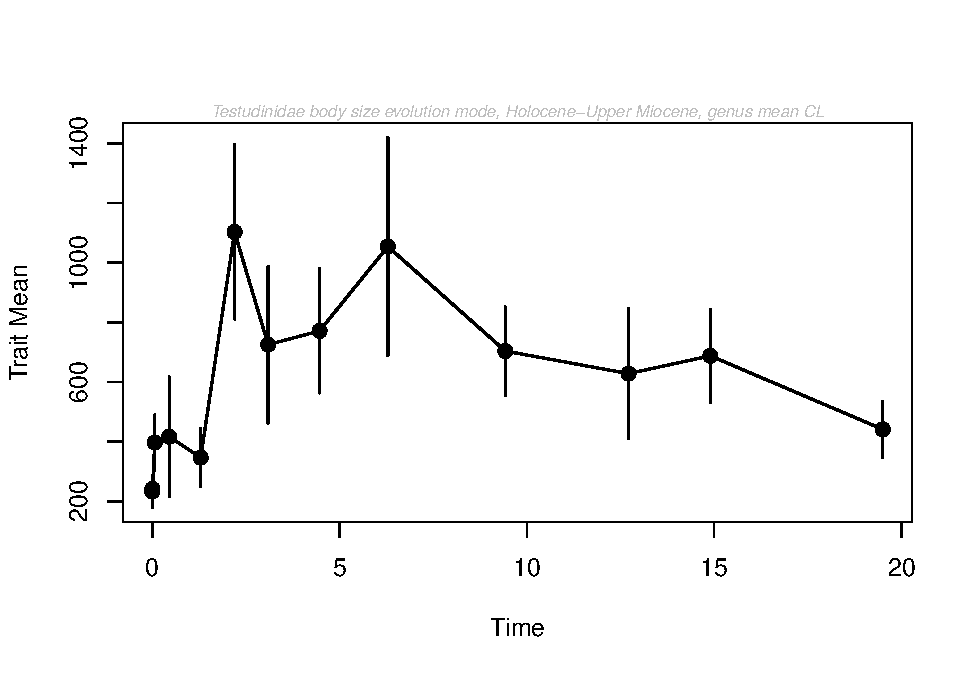
\includegraphics{MA_JJ_files/figure-latex/paleoTSC-1.pdf}
\caption{paleoTS plot with genus mean, continental}
\end{figure}

\begin{longtable}[]{@{}lrrrr@{}}
\caption{Model-fitting results for testudinidae, genera,
continental}\tabularnewline
\toprule
& logL & K & AICc & Akaike.wt\tabularnewline
\midrule
\endfirsthead
\toprule
& logL & K & AICc & Akaike.wt\tabularnewline
\midrule
\endhead
GRW & -77.27805 & 2 & 160.0561 & 0.077\tabularnewline
URW & -78.24092 & 1 & 158.9263 & 0.135\tabularnewline
Stasis & -74.94957 & 2 & 155.3991 & 0.788\tabularnewline
\bottomrule
\end{longtable}

\newpage

\subsection{insular (excluding
continental)}\label{insular-excluding-continental}

\subsubsection{genera (insular)}\label{genera-insular}

\begin{longtable}[]{@{}rrrr@{}}
\caption{paleoTS object, insular}\tabularnewline
\toprule
tt & nn & mm & vv\tabularnewline
\midrule
\endfirsthead
\toprule
tt & nn & mm & vv\tabularnewline
\midrule
\endhead
0.00585 & 13 & 416.5655 & 80682.22\tabularnewline
0.06885 & 4 & 727.5938 & 14997.58\tabularnewline
0.45350 & 3 & 748.8333 & 142649.08\tabularnewline
1.29350 & 6 & 829.6744 & 112964.44\tabularnewline
2.19700 & 3 & 1178.3333 & 821158.33\tabularnewline
3.09400 & 4 & 449.4375 & 27058.77\tabularnewline
4.46600 & 2 & 826.1667 & 15196.06\tabularnewline
6.28900 & 1 & 1850.0000 & 0.00\tabularnewline
\bottomrule
\end{longtable}

\begin{figure}[htbp]
\centering
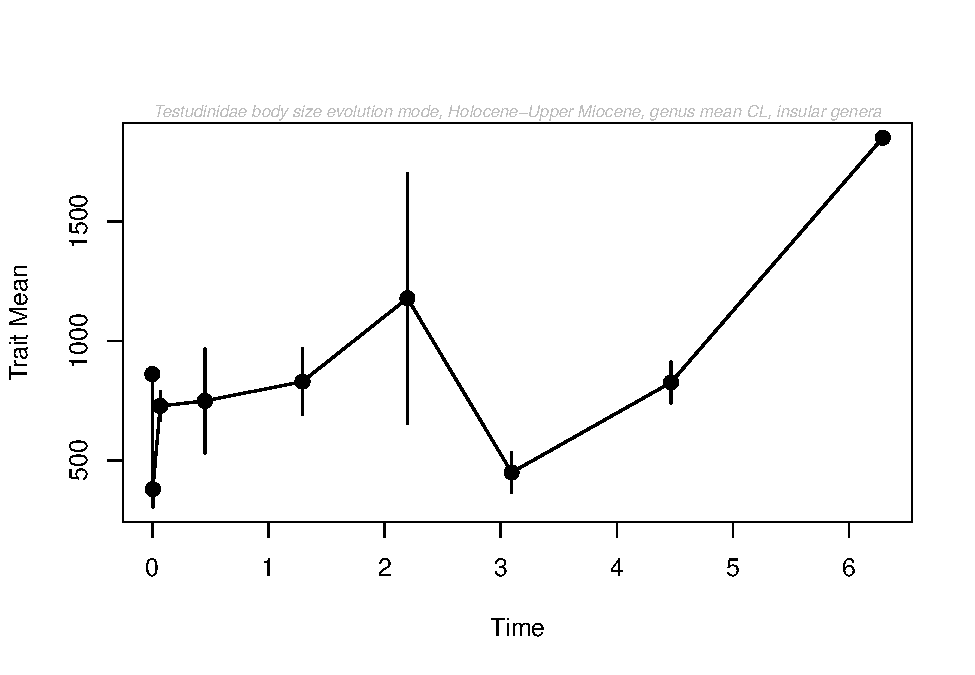
\includegraphics{MA_JJ_files/figure-latex/paleoTSI-1.pdf}
\caption{paleoTS plot with genus mean, insular}
\end{figure}

\begin{longtable}[]{@{}lrrrr@{}}
\caption{Model-fitting results for testudinidae, genera,
insular}\tabularnewline
\toprule
& logL & K & AICc & Akaike.wt\tabularnewline
\midrule
\endfirsthead
\toprule
& logL & K & AICc & Akaike.wt\tabularnewline
\midrule
\endhead
GRW & -52.51109 & 2 & 112.0222 & 0.230\tabularnewline
URW & -53.67334 & 1 & 110.1467 & 0.586\tabularnewline
Stasis & -52.73284 & 2 & 112.4657 & 0.184\tabularnewline
\bottomrule
\end{longtable}

\newpage

\subsection{per continent}\label{per-continent}

\subsubsection{Europe, genera}\label{europe-genera}

\begin{longtable}[]{@{}rrrr@{}}
\caption{paleoTS object, Europe}\tabularnewline
\toprule
tt & nn & mm & vv\tabularnewline
\midrule
\endfirsthead
\toprule
tt & nn & mm & vv\tabularnewline
\midrule
\endhead
0.00585 & 2 & 148.8559 & 3338.406\tabularnewline
0.06885 & 3 & 616.6667 & 138802.333\tabularnewline
0.45350 & 3 & 377.8167 & 89203.953\tabularnewline
1.29350 & 5 & 697.3717 & 218431.974\tabularnewline
2.19700 & 2 & 895.0000 & 1110050.000\tabularnewline
3.09400 & 3 & 453.3333 & 39433.333\tabularnewline
4.46600 & 5 & 1215.8667 & 159317.256\tabularnewline
6.28900 & 2 & 838.3750 & 875495.281\tabularnewline
9.42700 & 6 & 800.0508 & 263434.389\tabularnewline
12.71400 & 5 & 653.9625 & 351634.528\tabularnewline
14.89500 & 5 & 772.0000 & 223154.375\tabularnewline
19.50000 & 5 & 533.8533 & 183706.682\tabularnewline
\bottomrule
\end{longtable}

\begin{figure}[htbp]
\centering
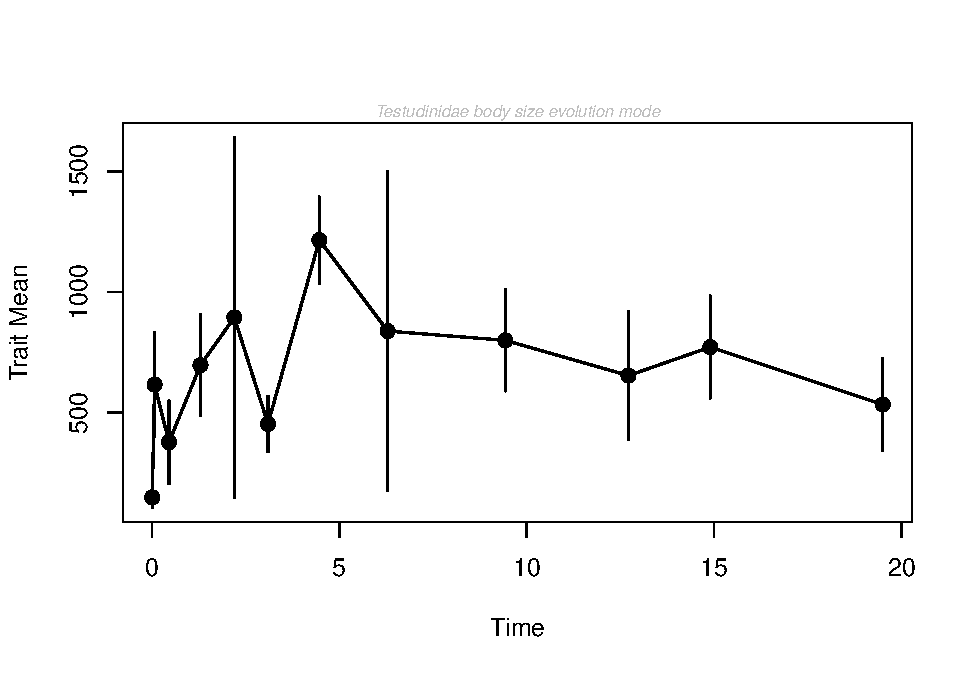
\includegraphics{MA_JJ_files/figure-latex/paleoTSEurope-1.pdf}
\caption{Genera, Europe}
\end{figure}

\begin{longtable}[]{@{}lrrrr@{}}
\caption{Model-fitting results for testudinidae, genera,
Europe}\tabularnewline
\toprule
& logL & K & AICc & Akaike.wt\tabularnewline
\midrule
\endfirsthead
\toprule
& logL & K & AICc & Akaike.wt\tabularnewline
\midrule
\endhead
GRW & -84.14010 & 2 & 173.7802 & 0.006\tabularnewline
URW & -85.90727 & 1 & 174.2590 & 0.005\tabularnewline
Stasis & -79.01365 & 2 & 163.5273 & 0.990\tabularnewline
\bottomrule
\end{longtable}

\newpage

\paragraph{Europe, smaller original bins (see Table 2), genera,
continental}\label{europe-smaller-original-bins-see-table-2-genera-continental}

\begin{longtable}[]{@{}rrrr@{}}
\caption{paleoTs object, Europe, continental}\tabularnewline
\toprule
tt & nn & mm & vv\tabularnewline
\midrule
\endfirsthead
\toprule
tt & nn & mm & vv\tabularnewline
\midrule
\endhead
0.00585 & 2 & 149.5381 & 3450.8267\tabularnewline
0.06885 & 1 & 187.0000 & 0.0000\tabularnewline
0.45350 & 2 & 205.4750 & 198.0050\tabularnewline
1.29350 & 2 & 204.9292 & 23.1767\tabularnewline
2.19700 & 1 & 1420.0000 & 0.0000\tabularnewline
3.09400 & 1 & 232.5000 & 0.0000\tabularnewline
4.46600 & 3 & 1475.6667 & 57926.3333\tabularnewline
6.28900 & 2 & 663.3750 & 473607.7812\tabularnewline
9.42700 & 6 & 800.0508 & 263434.3893\tabularnewline
12.71400 & 5 & 653.9625 & 351634.5281\tabularnewline
14.89500 & 5 & 772.0000 & 223154.3750\tabularnewline
19.50000 & 5 & 533.8533 & 183706.6821\tabularnewline
\bottomrule
\end{longtable}

\begin{figure}[htbp]
\centering
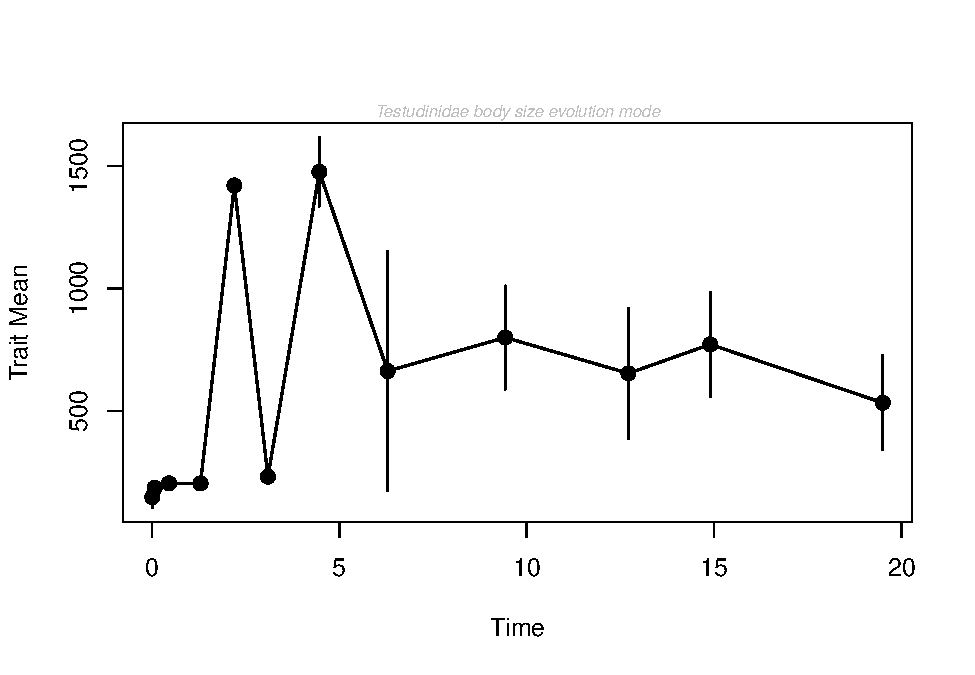
\includegraphics{MA_JJ_files/figure-latex/pTSEuC-1.pdf}
\caption{paleoTS, genera, Europe, continental}
\end{figure}

\begin{longtable}[]{@{}lrrrr@{}}
\caption{Model-fitting results for testudinidae, genera, Europe,
continental}\tabularnewline
\toprule
& logL & K & AICc & Akaike.wt\tabularnewline
\midrule
\endfirsthead
\toprule
& logL & K & AICc & Akaike.wt\tabularnewline
\midrule
\endhead
GRW & -87.93137 & 2 & 181.3627 & 0.009\tabularnewline
URW & -92.56882 & 1 & 187.5821 & 0.000\tabularnewline
Stasis & -83.21073 & 2 & 171.9215 & 0.991\tabularnewline
\bottomrule
\end{longtable}

\newpage

\paragraph{Europe, smaller original bins (see Table 2), genera,
insular}\label{europe-smaller-original-bins-see-table-2-genera-insular}

\begin{longtable}[]{@{}rrrr@{}}
\caption{paleoTs object, Europe, insular}\tabularnewline
\toprule
tt & nn & mm & vv\tabularnewline
\midrule
\endfirsthead
\toprule
tt & nn & mm & vv\tabularnewline
\midrule
\endhead
0.00585 & 1 & 187.5077 & 0.00\tabularnewline
0.06885 & 2 & 831.5000 & 684.50\tabularnewline
0.45350 & 1 & 722.5000 & 0.00\tabularnewline
1.29350 & 4 & 835.0833 & 168423.36\tabularnewline
2.19700 & 2 & 1005.0000 & 1462050.00\tabularnewline
3.09400 & 3 & 451.6667 & 40558.33\tabularnewline
4.46600 & 2 & 826.1667 & 15196.06\tabularnewline
6.28900 & 1 & 1850.0000 & 0.00\tabularnewline
\bottomrule
\end{longtable}

\begin{figure}[htbp]
\centering
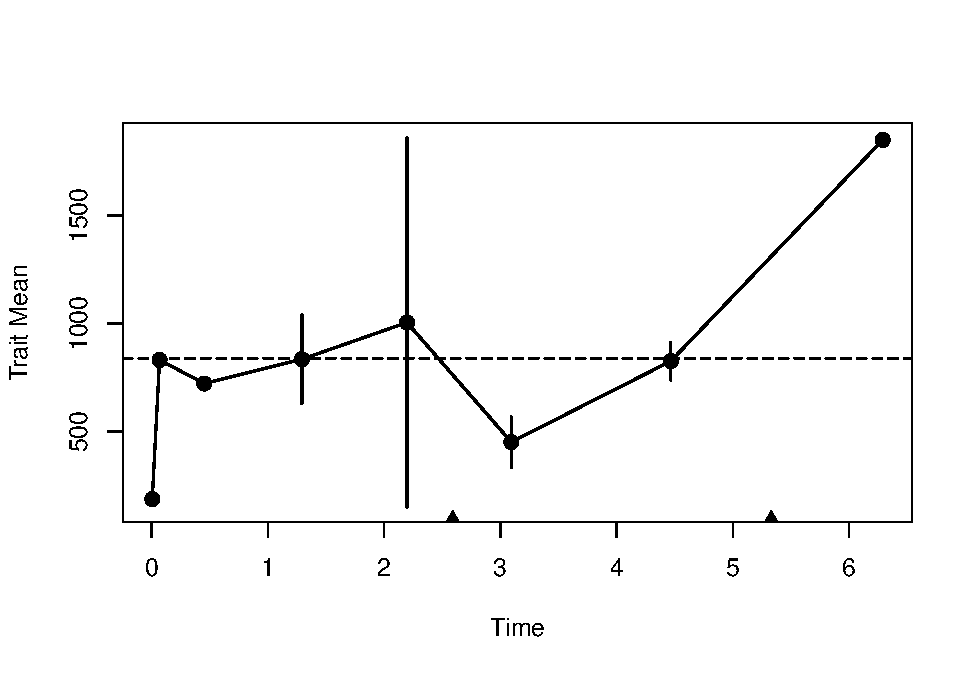
\includegraphics{MA_JJ_files/figure-latex/pTSEuI-1.pdf}
\caption{paleoTS, genera, Europe, insular}
\end{figure}

\begin{longtable}[]{@{}lrrrr@{}}
\caption{Model-fitting results for testudinidae, genera, Europe,
insular}\tabularnewline
\toprule
& logL & K & AICc & Akaike.wt\tabularnewline
\midrule
\endfirsthead
\toprule
& logL & K & AICc & Akaike.wt\tabularnewline
\midrule
\endhead
GRW & -67.12192 & 2 & 141.2438 & 0.000\tabularnewline
URW & -57.51634 & 1 & 117.8327 & 0.074\tabularnewline
Stasis & -52.89638 & 2 & 112.7928 & 0.926\tabularnewline
\bottomrule
\end{longtable}

\newpage 

\subsubsection{Eurasia, genera}\label{eurasia-genera}

\begin{longtable}[]{@{}rrrr@{}}
\caption{paleoTS object, all data, Eurasia}\tabularnewline
\toprule
tt & nn & mm & vv\tabularnewline
\midrule
\endfirsthead
\toprule
tt & nn & mm & vv\tabularnewline
\midrule
\endhead
0.00585 & 6 & 210.8687 & 10460.89\tabularnewline
0.06885 & 4 & 530.0000 & 122579.33\tabularnewline
0.45350 & 3 & 377.8167 & 89203.95\tabularnewline
1.29350 & 7 & 777.5579 & 162641.14\tabularnewline
2.19700 & 5 & 909.6667 & 562217.22\tabularnewline
3.09400 & 5 & 892.0000 & 381770.00\tabularnewline
4.46600 & 6 & 1048.0556 & 296417.22\tabularnewline
6.28900 & 3 & 1208.9167 & 849651.02\tabularnewline
9.42700 & 6 & 800.0508 & 263434.39\tabularnewline
12.71400 & 5 & 653.9625 & 351634.53\tabularnewline
14.89500 & 5 & 772.0000 & 223154.38\tabularnewline
19.50000 & 5 & 513.8533 & 162399.35\tabularnewline
\bottomrule
\end{longtable}

\begin{figure}[htbp]
\centering
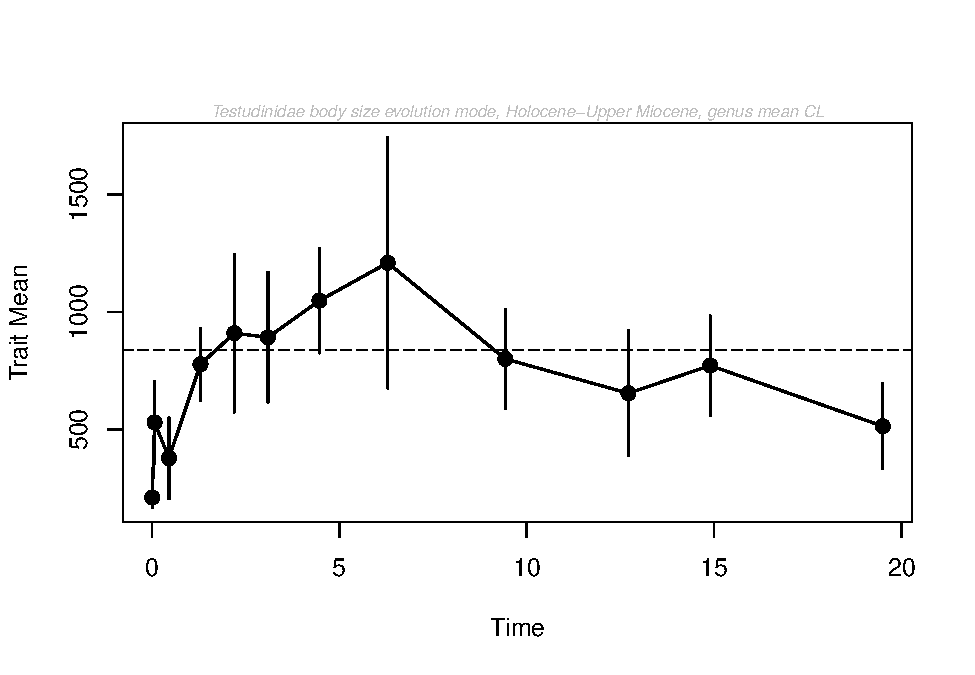
\includegraphics{MA_JJ_files/figure-latex/paleoTSEurasia-1.pdf}
\caption{paleoTS, genera, Eurasia}
\end{figure}

\begin{longtable}[]{@{}lrrrr@{}}
\caption{Model-fitting results for testudinidae, genera,
Eurasia}\tabularnewline
\toprule
& logL & K & AICc & Akaike.wt\tabularnewline
\midrule
\endfirsthead
\toprule
& logL & K & AICc & Akaike.wt\tabularnewline
\midrule
\endhead
GRW & -78.25066 & 2 & 162.0013 & 0.039\tabularnewline
URW & -78.39530 & 1 & 159.2350 & 0.154\tabularnewline
Stasis & -75.21099 & 2 & 155.9220 & 0.807\tabularnewline
\bottomrule
\end{longtable}

\newpage 

\subsubsection{Eurasia, genera,
continental}\label{eurasia-genera-continental}

\begin{longtable}[]{@{}rrrr@{}}
\caption{paleoTS object, all data}\tabularnewline
\toprule
tt & nn & mm & vv\tabularnewline
\midrule
\endfirsthead
\toprule
tt & nn & mm & vv\tabularnewline
\midrule
\endhead
0.00585 & 6 & 210.6223 & 10502.932\tabularnewline
0.06885 & 2 & 228.5000 & 3444.500\tabularnewline
0.45350 & 2 & 205.4750 & 198.005\tabularnewline
1.29350 & 4 & 595.5388 & 191487.404\tabularnewline
2.19700 & 4 & 1044.5833 & 442006.250\tabularnewline
3.09400 & 3 & 1110.8333 & 581102.083\tabularnewline
4.46600 & 4 & 1159.0000 & 439728.667\tabularnewline
6.28900 & 3 & 1092.2500 & 788605.188\tabularnewline
9.42700 & 6 & 800.0508 & 263434.389\tabularnewline
12.71400 & 5 & 653.9625 & 351634.528\tabularnewline
14.89500 & 5 & 772.0000 & 223154.375\tabularnewline
19.50000 & 5 & 513.8533 & 162399.349\tabularnewline
\bottomrule
\end{longtable}

\begin{figure}[htbp]
\centering
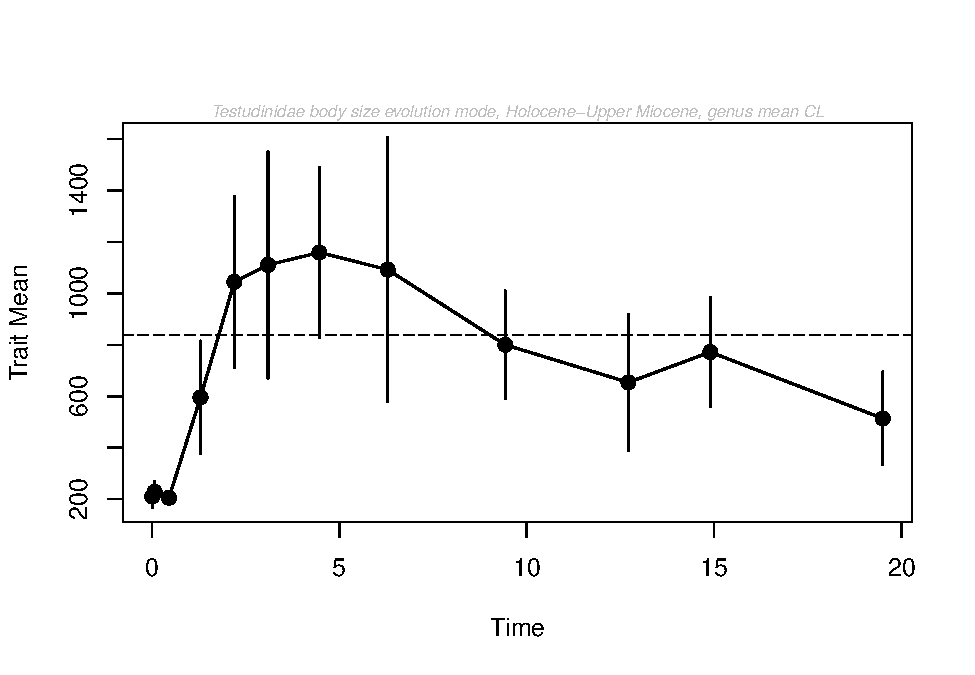
\includegraphics{MA_JJ_files/figure-latex/pTSEsC-1.pdf}
\caption{paleoTS, genera, Eurasia, continental}
\end{figure}

\begin{longtable}[]{@{}lrrrr@{}}
\caption{Model-fitting results for testudinidae, genera, Eurasia,
continental}\tabularnewline
\toprule
& logL & K & AICc & Akaike.wt\tabularnewline
\midrule
\endfirsthead
\toprule
& logL & K & AICc & Akaike.wt\tabularnewline
\midrule
\endhead
GRW & -74.89025 & 2 & 155.2805 & 0.211\tabularnewline
URW & -75.10165 & 1 & 152.6477 & 0.787\tabularnewline
Stasis & -79.85118 & 2 & 165.2024 & 0.001\tabularnewline
\bottomrule
\end{longtable}

\newpage 

\subsubsection{Eurasia, smaller original bins (See Table 2), genera,
insular}\label{eurasia-smaller-original-bins-see-table-2-genera-insular}

\begin{longtable}[]{@{}rrrr@{}}
\caption{paleoTS object, all data}\tabularnewline
\toprule
tt & nn & mm & vv\tabularnewline
\midrule
\endfirsthead
\toprule
tt & nn & mm & vv\tabularnewline
\midrule
\endhead
0.00585 & 4 & 272.9348 & 14139.94\tabularnewline
0.06885 & 2 & 831.5000 & 684.50\tabularnewline
0.45350 & 1 & 722.5000 & 0.00\tabularnewline
1.29350 & 5 & 876.4427 & 134870.49\tabularnewline
2.19700 & 3 & 1178.3333 & 821158.33\tabularnewline
3.09400 & 3 & 451.6667 & 40558.33\tabularnewline
4.46600 & 2 & 826.1667 & 15196.06\tabularnewline
6.28900 & 1 & 1850.0000 & 0.00\tabularnewline
\bottomrule
\end{longtable}

\begin{figure}[htbp]
\centering
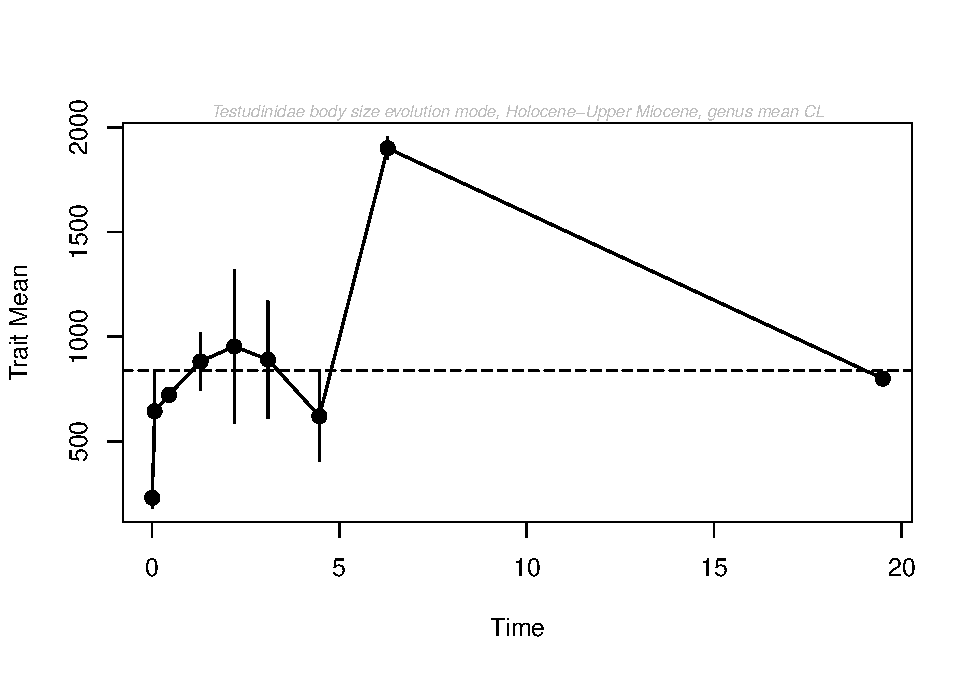
\includegraphics{MA_JJ_files/figure-latex/pTSEsI-1.pdf}
\caption{paleoTS, genera, Eurasia, insular}
\end{figure}

\begin{longtable}[]{@{}lrrrr@{}}
\caption{Model-fitting results for testudinidae, genera, Eurasia,
insular}\tabularnewline
\toprule
& logL & K & AICc & Akaike.wt\tabularnewline
\midrule
\endfirsthead
\toprule
& logL & K & AICc & Akaike.wt\tabularnewline
\midrule
\endhead
GRW & -56.16352 & 2 & 119.3270 & 0.027\tabularnewline
URW & -63.16971 & 1 & 129.1394 & 0.000\tabularnewline
Stasis & -52.56060 & 2 & 112.1212 & 0.973\tabularnewline
\bottomrule
\end{longtable}

\begin{longtable}[]{@{}llllrllrlll@{}}
\caption{Data set, fossil.}\tabularnewline
\toprule
& Locality & Genus & Taxon & CL & estimated & EpochBins & Age & Island &
Con & Reference\tabularnewline
\midrule
\endfirsthead
\toprule
& Locality & Genus & Taxon & CL & estimated & EpochBins & Age & Island &
Con & Reference\tabularnewline
\midrule
\endhead
1 & Laetoli, Tanzania & Aldabrachelys & ``Aldabrachelys'' laetoliensis &
1000.00 & mo & Piacencian & 2.70300 & n & Africa & Meylan and
Auffenberg, 1986\tabularnewline
2 & Sal Island & Centrochelys & Centrochelys atlantica & 400.00 & mo &
Lower Pleistocene & 1.30000 & y & Africa & Lopez-Jurado et al.,
1998\tabularnewline
3 & Ahl al Oughlam (near Casablanca) & Centrochelys & Centrochelys
marocana & 2050.00 & mo & Gelasian & 2.50000 & n & Africa & Lapparent de
Broin F.de, 2002a: A giant tortoise from the Late Pliocene of Lesvos
Island (Greece) and its possible relationships. Annales Geologiques des
Pays Helleniques, 1e Serie, t.XXXIX, fasc. A: 99-130\tabularnewline
4 & Kanapoi & Geochelone & Geochelone crassa & 865.00 & mf & Zanclean &
4.14500 & n & Africa & Harris et al., 2003\tabularnewline
5 & Djebel Krechem & Geochelone & Geochelone sp. & 1446.00 & eh &
Tortonian & 8.47600 & n & Africa & Geraads, 1989\tabularnewline
6 & Pellatal Phosphate Member, Varswater Formation, E Quarry
Langebaanweg & Geochelone & Geochelone stromeri & 350.00 & m & Zanclean
& 4.46600 & n & Africa & Meylan and Auffenberg, 1986\tabularnewline
7 & Pellatal Phosphate Member, Varswater Formation, E Quarry
Langebaanweg & Geochelone & Geochelone stromeri & 425.00 & m & Zanclean
& 4.46600 & n & Africa & Meylan and Auffenberg, 1986\tabularnewline
8 & South Africa & Homopus & Homopus fenestratus & 90.00 & mo &
Piacencian & 3.05650 & n & Africa & Rhodin et al., 2015\tabularnewline
9 & Rusinga Island, Lake Victoria, Kenya & Impregnochelys &
Impregnochelys pachytectis & 620.00 & m & Burdigalian/Aquitanian &
19.50000 & n & Africa & Meylan and Auffenberg, 1986\tabularnewline
10 & Arrisdrift & Mesocherus & Mesocherus orangeus & 160.00 & mo &
Burdigalian/Aquitanian & 17.25000 & n & Africa & Lapparent de Broin
F.de, 2003: Miocene Chelonians from southern Namibia. in: B. Senut \& M.
Pickford coord., Faunas from the southern Namibia. Memoir Geol. Surv.
Namibia 19: 67-102aus den Diamantfeldern Deutsch Südwestafrica. in: Die
Diamantenwüste Südwest-Afrikas, Erich Kaiser (ed.) 2: 139-141, D.
Reimer, Berlin\tabularnewline
11 & Arrisdrift & Mesocherus & Mesocherus orangeus & 180.00 & mo &
Burdigalian/Aquitanian & 17.25000 & n & Africa & Lapparent de Broin
F.de, 2003: Miocene Chelonians from southern Namibia. in: B. Senut \& M.
Pickford coord., Faunas from the southern Namibia. Memoir Geol. Surv.
Namibia 19: 67-102aus den Diamantfeldern Deutsch Südwestafrica. in: Die
Diamantenwüste Südwest-Afrikas, Erich Kaiser (ed.) 2: 139-141, D.
Reimer, Berlin\tabularnewline
12 & Arrisdrift & Mesocherus & Mesocherus orangeus & 180.00 & mo &
Burdigalian/Aquitanian & 17.25000 & n & Africa & Lapparent de Broin
F.de, 2003: Miocene Chelonians from southern Namibia. in: B. Senut \& M.
Pickford coord., Faunas from the southern Namibia. Memoir Geol. Surv.
Namibia 19: 67-102aus den Diamantfeldern Deutsch Südwestafrica. in: Die
Diamantenwüste Südwest-Afrikas, Erich Kaiser (ed.) 2: 139-141, D.
Reimer, Berlin\tabularnewline
13 & Arrisdrift & Mesocherus & Mesocherus orangeus & 180.00 & mo &
Burdigalian/Aquitanian & 17.25000 & n & Africa & Lapparent de Broin
F.de, 2003: Miocene Chelonians from southern Namibia. in: B. Senut \& M.
Pickford coord., Faunas from the southern Namibia. Memoir Geol. Surv.
Namibia 19: 67-102aus den Diamantfeldern Deutsch Südwestafrica. in: Die
Diamantenwüste Südwest-Afrikas, Erich Kaiser (ed.) 2: 139-141, D.
Reimer, Berlin\tabularnewline
14 & Arrisdrift & Mesocherus & Mesocherus orangeus & 180.00 & mo &
Burdigalian/Aquitanian & 17.25000 & n & Africa & Lapparent de Broin
F.de, 2003: Miocene Chelonians from southern Namibia. in: B. Senut \& M.
Pickford coord., Faunas from the southern Namibia. Memoir Geol. Surv.
Namibia 19: 67-102aus den Diamantfeldern Deutsch Südwestafrica. in: Die
Diamantenwüste Südwest-Afrikas, Erich Kaiser (ed.) 2: 139-141, D.
Reimer, Berlin\tabularnewline
15 & Arrisdrift & Mesocherus & Mesocherus orangeus & 180.00 & mo &
Burdigalian/Aquitanian & 17.25000 & n & Africa & Lapparent de Broin
F.de, 2003: Miocene Chelonians from southern Namibia. in: B. Senut \& M.
Pickford coord., Faunas from the southern Namibia. Memoir Geol. Surv.
Namibia 19: 67-102aus den Diamantfeldern Deutsch Südwestafrica. in: Die
Diamantenwüste Südwest-Afrikas, Erich Kaiser (ed.) 2: 139-141, D.
Reimer, Berlin\tabularnewline
16 & Arrisdrift & Mesocherus & Mesocherus orangeus & 200.00 & mo &
Burdigalian/Aquitanian & 17.25000 & n & Africa & Lapparent de Broin
F.de, 2003: Miocene Chelonians from southern Namibia. in: B. Senut \& M.
Pickford coord., Faunas from the southern Namibia. Memoir Geol. Surv.
Namibia 19: 67-102aus den Diamantfeldern Deutsch Südwestafrica. in: Die
Diamantenwüste Südwest-Afrikas, Erich Kaiser (ed.) 2: 139-141, D.
Reimer, Berlin\tabularnewline
17 & Arrisdrift & Namibchersus & Namibchersus aff. namaquensis & 1100.00
& mo & Burdigalian/Aquitanian & 17.25000 & n & Africa & Lapparent de
Broin F.de, 2003: Miocene Chelonians from southern Namibia. in: B. Senut
\& M. Pickford coord., Faunas from the southern Namibia. Memoir Geol.
Surv. Namibia 19: 67-102aus den Diamantfeldern Deutsch Südwestafrica.
in: Die Diamantenwüste Südwest-Afrikas, Erich Kaiser (ed.) 2: 139-141,
D. Reimer, Berlin\tabularnewline
18 & Arrisdrift & Namibchersus & Namibchersus aff. namaquensis & 440.00
& mo & Burdigalian/Aquitanian & 17.25000 & n & Africa & Lapparent de
Broin F.de, 2003: Miocene Chelonians from southern Namibia. in: B. Senut
\& M. Pickford coord., Faunas from the southern Namibia. Memoir Geol.
Surv. Namibia 19: 67-102aus den Diamantfeldern Deutsch Südwestafrica.
in: Die Diamantenwüste Südwest-Afrikas, Erich Kaiser (ed.) 2: 139-141,
D. Reimer, Berlin\tabularnewline
19 & Arrisdrift & Namibchersus & Namibchersus aff. namaquensis & 550.00
& mo & Burdigalian/Aquitanian & 17.25000 & n & Africa & Lapparent de
Broin F.de, 2003: Miocene Chelonians from southern Namibia. in: B. Senut
\& M. Pickford coord., Faunas from the southern Namibia. Memoir Geol.
Surv. Namibia 19: 67-102aus den Diamantfeldern Deutsch Südwestafrica.
in: Die Diamantenwüste Südwest-Afrikas, Erich Kaiser (ed.) 2: 139-141,
D. Reimer, Berlin\tabularnewline
20 & Auchas & Namibchersus & Namibchersus namaquensis & 254.00 & m &
Burdigalian/Aquitanian & 18.00000 & n & Africa & Lapparent de Broin
F.de, 2003: Miocene Chelonians from southern Namibia. in: B. Senut \& M.
Pickford coord., Faunas from the southern Namibia. Memoir Geol. Surv.
Namibia 19: 67-102aus den Diamantfeldern Deutsch Südwestafrica. in: Die
Diamantenwüste Südwest-Afrikas, Erich Kaiser (ed.) 2: 139-141, D.
Reimer, Berlin\tabularnewline
21 & Elisabethfeld (= Elisabeth Bay) area, northern Sperrgebiet &
Namibchersus & Namibchersus namaquensis & 264.00 & m &
Burdigalian/Aquitanian & 19.50000 & n & Africa & Lapparent de Broin
F.de, 2003: Miocene Chelonians from southern Namibia. in: B. Senut \& M.
Pickford coord., Faunas from the southern Namibia. Memoir Geol. Surv.
Namibia 19: 67-102aus den Diamantfeldern Deutsch Südwestafrica. in: Die
Diamantenwüste Südwest-Afrikas, Erich Kaiser (ed.) 2: 139-141, D.
Reimer, Berlin\tabularnewline
22 & Elisabethfeld (= Elisabeth Bay) area, northern Sperrgebiet &
Namibchersus & Namibchersus namaquensis & 300.00 & m &
Burdigalian/Aquitanian & 19.50000 & n & Africa & Lapparent de Broin
F.de, 2003: Miocene Chelonians from southern Namibia. in: B. Senut \& M.
Pickford coord., Faunas from the southern Namibia. Memoir Geol. Surv.
Namibia 19: 67-102aus den Diamantfeldern Deutsch Südwestafrica. in: Die
Diamantenwüste Südwest-Afrikas, Erich Kaiser (ed.) 2: 139-141, D.
Reimer, Berlin\tabularnewline
23 & Auchas & Namibchersus & Namibchersus namaquensis & 470.00 & m &
Burdigalian/Aquitanian & 18.00000 & n & Africa & Lapparent de Broin
F.de, 2003: Miocene Chelonians from southern Namibia. in: B. Senut \& M.
Pickford coord., Faunas from the southern Namibia. Memoir Geol. Surv.
Namibia 19: 67-102aus den Diamantfeldern Deutsch Südwestafrica. in: Die
Diamantenwüste Südwest-Afrikas, Erich Kaiser (ed.) 2: 139-141, D.
Reimer, Berlin\tabularnewline
24 & Auchas & Namibchersus & Namibchersus namaquensis & 470.00 & m &
Burdigalian/Aquitanian & 18.00000 & n & Africa & Lapparent de Broin
F.de, 2003: Miocene Chelonians from southern Namibia. in: B. Senut \& M.
Pickford coord., Faunas from the southern Namibia. Memoir Geol. Surv.
Namibia 19: 67-102aus den Diamantfeldern Deutsch Südwestafrica. in: Die
Diamantenwüste Südwest-Afrikas, Erich Kaiser (ed.) 2: 139-141, D.
Reimer, Berlin\tabularnewline
25 & Auchas & Namibchersus & Namibchersus namaquensis & 815.00 & m &
Burdigalian/Aquitanian & 18.00000 & n & Africa & Lapparent de Broin
F.de, 2003: Miocene Chelonians from southern Namibia. in: B. Senut \& M.
Pickford coord., Faunas from the southern Namibia. Memoir Geol. Surv.
Namibia 19: 67-102aus den Diamantfeldern Deutsch Südwestafrica. in: Die
Diamantenwüste Südwest-Afrikas, Erich Kaiser (ed.) 2: 139-141, D.
Reimer, Berlin\tabularnewline
26 & Drimolon, Sterkfontein, Krugersdorp District, Gauteng Province &
Psammobates & Psammobates antiquorum & 107.80 & m & Lower Pleistocene &
1.80000 & n & Africa & Broadley, 1997\tabularnewline
27 & Ahl al Oughlam (near Casablanca) & Testudo & Testudo aff.
kenitrensis & 142.00 & mf & Gelasian & 2.50000 & n & Africa & Gmira s.,
2013\tabularnewline
28 & Kénitra, Guilloux quarry, near Rabat & Testudo & Testudo
kenitrensis & 132.00 & mo & Middle Pleistocene & 0.45350 & n & Africa &
Gmira S., 1993: Une nouvelle espèce de tortue Testudininei (Testudo
kenitrensis n. sp.) de l'Inter Amirien-Tensiftien de Kénitra (Maroc).
Comptes rendus de l'Académie des Sciences de Paris -II 316:
701-707\tabularnewline
29 & Ahl al Oughlam (near Casablanca) & Testudo & Testudo oughlamensis &
120.00 & mo & Gelasian & 2.50000 & n & Africa & Gmira s.,
2013\tabularnewline
30 & Ahl al Oughlam (near Casablanca) & Testudo & Testudo sp. & 184.00 &
mf & Gelasian & 2.50000 & n & Africa & Gmira s., 2013\tabularnewline
31 & Ahl al Oughlam (near Casablanca) & Testudo & Testudo sp. & 200.00 &
mf & Gelasian & 2.50000 & n & Africa & Gmira s., 2013\tabularnewline
32 & Tha Chang area, Chaloem Pra Kiat district, Nakhon Ratchasima
Province & Aldabrachelys & Aldabrachelys ? sp. & 1500.00 & mo &
Piacencian & 3.00000 & n & Asia & Claude J., Naksri W., Boonchai N.,
Buffetaut E., Duangkrayom J., Laojumpon C., Jintasakul P., Lauprasert
K., Martin J., Sutheethorn V., Tong H., 2011: Neogene reptiles of
northeastern Thailand and their paleogeographical significance. Annales
de Paléontologie (2011)
\url{doi:10.1016/j.annpal.2011.08.002}\tabularnewline
33 & Tha Chang area, Chaloem Pra Kiat district, Nakhon Ratchasima
Province & Aldabrachelys & Aldabrachelys ? sp. & 1500.00 & mo &
Piacencian & 3.00000 & n & Asia & Claude J., Naksri W., Boonchai N.,
Buffetaut E., Duangkrayom J., Laojumpon C., Jintasakul P., Lauprasert
K., Martin J., Sutheethorn V., Tong H., 2011: Neogene reptiles of
northeastern Thailand and their paleogeographical significance. Annales
de Paléontologie (2011)
\url{doi:10.1016/j.annpal.2011.08.002}\tabularnewline
34 & Tha Chang area, Chaloem Pra Kiat district, Nakhon Ratchasima
Province & Aldabrachelys & Aldabrachelys ? sp. & 1500.00 & mo &
Piacencian & 3.00000 & n & Asia & Claude J., Naksri W., Boonchai N.,
Buffetaut E., Duangkrayom J., Laojumpon C., Jintasakul P., Lauprasert
K., Martin J., Sutheethorn V., Tong H., 2011: Neogene reptiles of
northeastern Thailand and their paleogeographical significance. Annales
de Paléontologie (2011)
\url{doi:10.1016/j.annpal.2011.08.002}\tabularnewline
35 & Tha Chang area, Chaloem Pra Kiat district, Nakhon Ratchasima
Province & Aldabrachelys & Aldabrachelys ? sp. & 1500.00 & mo &
Piacencian & 3.00000 & n & Asia & Claude J., Naksri W., Boonchai N.,
Buffetaut E., Duangkrayom J., Laojumpon C., Jintasakul P., Lauprasert
K., Martin J., Sutheethorn V., Tong H., 2011: Neogene reptiles of
northeastern Thailand and their paleogeographical significance. Annales
de Paléontologie (2011)
\url{doi:10.1016/j.annpal.2011.08.002}\tabularnewline
36 & Altan-Teli main fossiliferous bed (Dzereg valley) & Ergilemys &
Ergilemys oskarkuhni & 198.00 & m & Zanclean & 3.95000 & n & Asia &
Mlynarski, 1968: Notes on tortoises (Testudinidae) from the tertiary of
Mongolia. Paleontologica Polonica, 19: 85-99\tabularnewline
37 & Altan-Teli main fossiliferous bed (Dzereg valley) & Ergilemys &
Ergilemys oskarkuhni & 220.00 & m & Zanclean & 3.95000 & n & Asia &
Mlynarski, 1968: Notes on tortoises (Testudinidae) from the tertiary of
Mongolia. Paleontologica Polonica, 19: 85-99\tabularnewline
38 & Guangxi & gen. & gen. indet. & 900.00 & mo & Lower Pleistocene &
1.68450 & n & Asia & Rhodin et al., 2015\tabularnewline
39 & Ghaba & Geochelone & Geochelone sp. & 800.00 & ev &
Burdigalian/Aquitanian & 16.50000 & n & Asia & Roger,
1994\tabularnewline
40 & Lang Rongrien Rockshelter, Krabi, Thailand & Indotestudo &
Indotestudo elongata & 270.00 & m & Upper Pleistocene & 0.03700 & n &
Asia & Mudar and Anderson, 2007\tabularnewline
41 & Punjab & Manouria & Manouria punjabiensis & 900.00 & mo & Gelasian
& 2.19050 & n & Asia & Rhodin et al., 2015\tabularnewline
42 & Sulawesi (Celebes), Indonesia & Megalochelys & Megalochelys atlas &
1400.00 & mo & Gelasian & 2.00000 & y & Asia & Hooijer,
1951\tabularnewline
43 & Northwest of Naipli & Megalochelys & Megalochelys atlas & 1600.00 &
mo & Piacencian & 3.09400 & n & Asia & Badam, 1981\tabularnewline
44 & Northwest of Naipli & Megalochelys & Megalochelys atlas & 1600.00 &
mo & Piacencian & 3.09400 & n & Asia & Badam, 1981\tabularnewline
45 & Northwest of Naipli & Megalochelys & Megalochelys atlas & 1600.00 &
mo & Piacencian & 3.09400 & n & Asia & Badam, 1981\tabularnewline
46 & Northwest of Naipli & Megalochelys & Megalochelys atlas & 1600.00 &
mo & Piacencian & 3.09400 & n & Asia & Badam, 1981\tabularnewline
47 & Sulawesi (Celebes), Indonesia & Megalochelys & Megalochelys atlas &
1650.00 & mo & Gelasian & 2.00000 & y & Asia & Setiyabudi,
2009\tabularnewline
48 & Pauk Twonship & Megalochelys & Megalochelys atlas & 1800.00 & m &
Messinian & 5.42300 & n & Asia & Hirayama, R., Sonoda, T., Takai, M.,
Htike, T., Thein, Z. M. M., \& Takahashi, A. (2015).~Megalochelys:
gigantic tortoise from the Neogene of Myanmar~(No. e1185). PeerJ
PrePrints.\tabularnewline
49 & Siwalik & Megalochelys & Megalochelys atlas & 2000.00 & mo &
Gelasian & 2.19050 & n & Asia & Setiyabudi, 2009\tabularnewline
50 & Pauk Twonship & Megalochelys & Megalochelys atlas & 2100.00 & mo &
Messinian & 5.42300 & n & Asia & Hirayama, R., Sonoda, T., Takai, M.,
Htike, T., Thein, Z. M. M., \& Takahashi, A. (2015).~Megalochelys:
gigantic tortoise from the Neogene of Myanmar~(No. e1185). PeerJ
PrePrints.\tabularnewline
51 & Tres Hermanas, Manila, Luzon & Megalochelys & Megalochelys sondaari
& 1000.00 & ec & Lower Pleistocene & 1.35000 & y & Asia & Karl, H., \&
Staesche, U. (2007). Fossile Riesen-Landschildkroten von den Philippinen
und ihre palaogeographische Bedeutung. Geologisches Jahrbuch Reihe B,
98, 171.\tabularnewline
52 & Tres Hermanas, Manila, Luzon & Megalochelys & Megalochelys sondaari
& 818.00 & ec & Lower Pleistocene & 1.35000 & y & Asia & Karl, H., \&
Staesche, U. (2007). Fossile Riesen-Landschildkroten von den Philippinen
und ihre palaogeographische Bedeutung. Geologisches Jahrbuch Reihe B,
98, 171.\tabularnewline
53 & Flores & Megalochelys & Megalochelys sp. & 1200.00 & ev & Lower
Pleistocene & 0.90000 & y & Asia & Setiyabudi, 2009\tabularnewline
54 & Bumiayu, Java Island & Megalochelys & Megalochelys sp. & 191.40 & m
& Lower Pleistocene & 1.68450 & y & Asia & Setiyabudi,
2009\tabularnewline
55 & Java Island & Megalochelys & Megalochelys sp. & 2000.00 & m & Lower
Pleistocene & 1.68450 & y & Asia & Hirayama, R., Sonoda, T., Takai, M.,
Htike, T., Thein, Z. M. M., \& Takahashi, A. (2015).~Megalochelys:
gigantic tortoise from the Neogene of Myanmar~(No. e1185). PeerJ
PrePrints.\tabularnewline
56 & Zhejiang & Testudo & Testudo changshanesis & 330.00 & mo & Lower
Pleistocene & 1.68450 & n & Asia & Rhodin et al., 2015\tabularnewline
57 & Khatlon & Testudo & Testudo ranovi & 200.00 & mo & Gelasian &
2.19050 & n & Asia & Rhodin et al., 2015\tabularnewline
58 & Gerogia (Caucasus) & Testudo & Testudo transcaucasia & 150.00 & mo
& Gelasian & 2.19050 & n & Asia & Rhodin et al., 2015\tabularnewline
59 & Sawmill Sink, Abaco & Chelonoidis & Chelonoidis alburyorum & 424.00
& m & Piacencian & 3.20150 & y & America & Franz, R., \& Franz, S. E.
(2009). A new fossil land tortoise in the genus Chelonoidis (Testudines:
Testudinidae) from the Northern Bahamas: with an osteological assessment
of other neotropical tortoises. University of Florida.\tabularnewline
60 & Sawmill Sink, Abaco & Chelonoidis & Chelonoidis alburyorum & 428.00
& m & Piacencian & 3.20150 & y & America & Franz, R., \& Franz, S. E.
(2009). A new fossil land tortoise in the genus Chelonoidis (Testudines:
Testudinidae) from the Northern Bahamas: with an osteological assessment
of other neotropical tortoises. University of Florida.\tabularnewline
61 & Sawmill Sink, Abaco & Chelonoidis & Chelonoidis alburyorum & 453.00
& m & Piacencian & 3.20150 & y & America & Franz, R., \& Franz, S. E.
(2009). A new fossil land tortoise in the genus Chelonoidis (Testudines:
Testudinidae) from the Northern Bahamas: with an osteological assessment
of other neotropical tortoises. University of Florida.\tabularnewline
62 & Sawmill Sink, Abaco & Chelonoidis & Chelonoidis alburyorum & 466.00
& m & Piacencian & 3.20150 & y & America & Franz, R., \& Franz, S. E.
(2009). A new fossil land tortoise in the genus Chelonoidis (Testudines:
Testudinidae) from the Northern Bahamas: with an osteological assessment
of other neotropical tortoises. University of Florida.\tabularnewline
63 & Santa Clara & Chelonoidis & Chelonoidis cubensis & 1139.00 & ef &
Middle Pleistocene & 0.39350 & y & America & Williams, E. E. (1950).
Testudo cubensis and the evolution of western hemisphere tortoises.
Bulletin of the AMNH; v. 95, article 1.\tabularnewline
64 & Cueva del Papayo, Pedernales & Chelonoidis & Chelonoidis marcanoi &
530.00 & eh & Upper Pleistocene & 0.06900 & y & America & Turvey, S. T.,
Almonte, J., Hansford, J., Scofield, R. P., Brocca, J. L., \& Chapman,
S. D. (2017). A new species of extinct Late Quaternary giant tortoise
from Hispaniola.~Zootaxa,~4277(1), 1-16.\tabularnewline
65 & Cueva del Papayo, Pedernales & Chelonoidis & Chelonoidis marcanoi &
614.00 & eh & Upper Pleistocene & 0.06900 & y & America & Turvey, S. T.,
Almonte, J., Hansford, J., Scofield, R. P., Brocca, J. L., \& Chapman,
S. D. (2017). A new species of extinct Late Quaternary giant tortoise
from Hispaniola.~Zootaxa,~4277(1), 1-16.\tabularnewline
66 & Cueva del Papayo, Pedernales & Chelonoidis & Chelonoidis marcanoi &
767.00 & eh & Upper Pleistocene & 0.06900 & y & America & Turvey, S. T.,
Almonte, J., Hansford, J., Scofield, R. P., Brocca, J. L., \& Chapman,
S. D. (2017). A new species of extinct Late Quaternary giant tortoise
from Hispaniola.~Zootaxa,~4277(1), 1-16.\tabularnewline
67 & Cueva del Papayo, Pedernales & Chelonoidis & Chelonoidis marcanoi &
778.00 & eh & Upper Pleistocene & 0.06900 & y & America & Turvey, S. T.,
Almonte, J., Hansford, J., Scofield, R. P., Brocca, J. L., \& Chapman,
S. D. (2017). A new species of extinct Late Quaternary giant tortoise
from Hispaniola.~Zootaxa,~4277(1), 1-16.\tabularnewline
68 & Mona Island & Chelonoidis & Chelonoidis monensis & 500.00 & m &
Upper Pleistocene & 0.06450 & y & America & Williams,
1952\tabularnewline
69 & Sombrero Island & Chelonoidis & Chelonoidis sombrerensis & 990.00 &
m & Upper Pleistocene & 0.06900 & y & America & Carlson, L. A. (2000).
Aftermath of a feast: Human colonization of the southern Bahamian
archipelago and its effects on the indigenous fauna.\tabularnewline
70 & Navassa Island & Chelonoidis & Chelonoidis sp. & 400.00 & mo &
Upper Pleistocene & 0.06900 & y & America & Auffenberg, W. (1967). Notes
on West Indian tortoises. Herpetologica, 23(1), 34-44.\tabularnewline
71 & San Pedro, Curaçao & Chelonoidis & Chelonoidis sp. & 600.00 & mo &
Lower Pleistocene & 1.35700 & y & America & Hooijer, D. A. (1963).
Geochelone from the Pleistocene of Curaçao, Netherlands Antilles.
Copeia, 3, 579-580.\tabularnewline
72 & Bayaguana, Los Haitises, San Cristobal & Chelonoidis & Chelonoidis
sp. & 600.00 & mo & Upper Pleistocene & 0.06900 & y & America & Franz,
R., \& Woods, C. A. (1983). A fossil tortoise from Hispaniola. Journal
of Herpetology, 17(1), 79-81.\tabularnewline
73 & San Pedro, Curaçao & Chelonoidis & Chelonoidis sp. & 750.00 & mo &
Lower Pleistocene & 1.35700 & y & America & Hooijer, D. A. (1963).
Geochelone from the Pleistocene of Curaçao, Netherlands Antilles.
Copeia, 3, 579-580.\tabularnewline
74 & San Pedro, Curaçao & Chelonoidis & Chelonoidis sp. & 800.00 & mo &
Lower Pleistocene & 1.35700 & y & America & Hooijer, D. A. (1963).
Geochelone from the Pleistocene of Curaçao, Netherlands Antilles.
Copeia, 3, 579-580.\tabularnewline
75 & Cedazo local fauna, Aguascalientes, Mexico & Geochelone &
Geochelone sp. & 340.00 & mo & Lower Pleistocene & 1.05000 & n & America
& Mooser, 1972\tabularnewline
76 & Cedazo local fauna, Aguascalientes, Mexico & Gopherus & Gopherus
berlandieri & 195.00 & m & Lower Pleistocene & 1.05000 & n & America &
Mooser, 1972\tabularnewline
77 & Cedazo local fauna, Aguascalientes, Mexico & Gopherus & Gopherus
berlandieri & 256.30 & m & Lower Pleistocene & 1.05000 & n & America &
Mooser, 1972\tabularnewline
78 & Cedazo local fauna, Aguascalientes, Mexico & Gopherus & Gopherus
flavomarginatus & 450.00 & m & Lower Pleistocene & 1.05000 & n & America
& Mooser, 1972\tabularnewline
79 & Smith's Parrish, No. 3Verdmont Valley Close & Hesperotestudo &
Hesperotestudo bermudae & 270.00 & m & Middle Pleistocene & 0.31000 & y
& America & Meylan and Sterrer, 2000\tabularnewline
80 & Smith's Parrish, No. 3Verdmont Valley Close & Hesperotestudo &
Hesperotestudo bermudae & 500.00 & m & Middle Pleistocene & 0.31000 & y
& America & Olson and Meylan, 2009\tabularnewline
81 & Río Tomayate, Apopa Municipality & Hesperotestudo & Hesperotestudo
sp. & 1500.00 & mo & Lower Pleistocene & 0.96600 & n & America &
Cisneros, 2005\tabularnewline
82 & Belomechetskaya & Ergilemys & Ergilemys sp. & 1000.00 & m &
Langhian & 14.00000 & n & Europe & FosFarBase\tabularnewline
83 & Dmanisi & Testudo & Testudo graeca & 195.00 & mf & Lower
Pleistocene & 1.77000 & n & Europe & Blain H.A., Agustí H.,
Lordkipanidze D., Rook L., Delfino M., 2014: Paleoclimatic and
paleoenvironmental context of the Early Pleistocene hominins from
Dmanisi (Georgia, Lesser Caucasus) inferred from the herpetofaunal
assemblage. Quaternary Science Reviews 105: 136-150\tabularnewline
84 & Prottes & ``Hadrianus'' & ``Hadrianus sp.'' & 1000.00 & m &
Tortonian & 8.30000 & n & Europe & Bachmayer F., M?ynarski M., 1985: Die
Landschildkröten (Testudinidae) aus den Schotter-Ablagerungen (Pontien)
von Prottes, Niederösterreich.. Annalen des Naturhistorischen Museums in
Wien 87 A: 65-77\tabularnewline
85 & Adeje, Tenerife & Centrochelys & Centrochelys burchardi & 500.00 &
mo & Middle Pleistocene & 0.43500 & y & Europe & Ahl, E. (1925). Über
eine ausgestorbene Riesenschildkröte der Insel Teneriffa. Zeitschrift
der Deutschen Geologischen Gesellschaft, 575-580.\tabularnewline
86 & Callao de Fañabé, Tenerife & Centrochelys & Centrochelys burchardi
& 650.00 & mo & Middle Pleistocene & 0.43500 & y & Europe & Hutterer et
al., 1998\tabularnewline
87 & Adeje, Tenerife & Centrochelys & Centrochelys burchardi & 800.00 &
m & Middle Pleistocene & 0.43500 & y & Europe & Ahl, E. (1925). Über
eine ausgestorbene Riesenschildkröte der Insel Teneriffa. Zeitschrift
der Deutschen Geologischen Gesellschaft, 575-580.\tabularnewline
88 & Callao de Fañabé, Tenerife & Centrochelys & Centrochelys burchardi
& 940.00 & mo & Middle Pleistocene & 0.43500 & y & Europe & Hutterer et
al., 1998\tabularnewline
89 & Corrida, Malta & Centrochelys & Centrochelys robusta & 1100.00 & mo
& Zanclean & 4.91700 & y & Europe & Adams A.L., 1877: On gigantic
land-tortoises and a small freshwater species from the ossiferous
caverns of Malta, together with a list of their fossil fauna; and a note
on Chelonian remains from the rock-cavities of Gibraltar. Quarterly
Journal of the Geological Society of London 33: 177-191\tabularnewline
90 & Ghar Dalam & Centrochelys & Centrochelys robusta & 1200.00 & ev &
Lower Pleistocene & 1.30000 & y & Europe & Hunt and Schembri,
1999\tabularnewline
91 & Ghar Dalam & Centrochelys & Centrochelys robusta & 600.00 & ev &
Lower Pleistocene & 1.30000 & y & Europe & Hunt and Schembri,
1999\tabularnewline
92 & Mnaidra Gap, Malta & Centrochelys & Centrochelys robusta & 790.00 &
ef & Zanclean & 4.91700 & y & Europe & Adams A.L., 1877: On gigantic
land-tortoises and a small freshwater species from the ossiferous
caverns of Malta, together with a list of their fossil fauna; and a note
on Chelonian remains from the rock-cavities of Gibraltar. Quarterly
Journal of the Geological Society of London 33: 177-191\tabularnewline
93 & Corrida, Malta & Centrochelys & Centrochelys robusta & 850.00 & mo
& Zanclean & 4.91700 & y & Europe & Adams A.L., 1877: On gigantic
land-tortoises and a small freshwater species from the ossiferous
caverns of Malta, together with a list of their fossil fauna; and a note
on Chelonian remains from the rock-cavities of Gibraltar. Quarterly
Journal of the Geological Society of London 33: 177-191\tabularnewline
94 & Zebbug and Gahr Dalam Cave deposits & Centrochelys & Centrochelys
robusta & 850.00 & mo & Upper Pleistocene & 0.06600 & y & Europe &
Lapparent de Broin F.de, 2002a: A giant tortoise from the Late Pliocene
of Lesvos Island (Greece) and its possible relationships. Annales
Geologiques des Pays Helleniques, 1e Serie, t.XXXIX, fasc. A:
99-130\tabularnewline
95 & Ghar Dalam & Centrochelys & Centrochelys robusta & 850.00 & ev &
Lower Pleistocene & 1.30000 & y & Europe & Hunt and Schembri,
1999\tabularnewline
96 & Barranco de las Ballenas, Las Palmas, Gran Canaria & Centrochelys &
Centrochelys vulcanica & 610.00 & mo & Piacencian & 3.09400 & y & Europe
& Hutterer et al., 1998\tabularnewline
97 & Pujo d'es Fum, Formentera, Balearic Islands & Cheirogaster &
Cheirogaster cf.~gymnesica & 789.00 & mo & Lower Pleistocene & 1.80000 &
y & Europe & Filella-Subira et al., 1999\tabularnewline
98 & Punta Nati near Ciutadella, Minorca & Cheirogaster & Cheirogaster
gymnesica & 739.00 & ef & Zanclean & 4.45000 & y & Europe & Mercadal B.,
Pretus Real L., 1980: Nuevo yacimiento de Testudo gymnesicus Bate, 1914
en la isla de Menorca. Boletín de la Sociedad de Historia Natural de
Baleares 24: 15-21\tabularnewline
99 & Hostalets de Piérola, Barcelone province, Cataluña, Vallés-Penedés
basin & Cheirogaster & Cheirogaster richardi & 1155.00 & mo & Tortonian
& 10.40000 & n & Europe & Pérez-García A., Vlachos E., 2014: New generic
proposal for the European Neogene large testudinids (Cryptodira) and the
?rst phylogenetic hypothesis for the medium and large representatives of
the European Cenozoic record. Zoological Journal of the Linnean Society
172: 653-719\tabularnewline
100 & La Ciesma 1, Aragón & Cheirogaster & Cheirogaster sp. & 1000.00 &
mo & Serravallian & 12.20000 & n & Europe & Murelaga X., Azanza B.,
Astibia H., 2006: Restos de quelonios del Mioceno medio del área de
Tarazona de Aragón (Cuenca del Ebro, Aragón, España). Estudios
Geológicos 62(1): 205-212\tabularnewline
101 & El Lugarejo (Arévalo), Ávilla, Castilla & Cheirogaster &
Cheirogaster sp. & 1170.00 & m & Tortonian & 10.25000 & n & Europe &
Jiménez Fuentes, E., Acosta, P., \& Fincias San Martín, B. (1986). Un
nuevo ejemplar de tortuga gigante del Mioceno de Arévalo (Ávila). Studia
Geologica. Salmanticensia, 23, 11.\tabularnewline
102 & Chañe, Segovia & Cheirogaster & Cheirogaster sp. & 1500.00 & e &
Serravallian & 13.80000 & n & Europe & Jiménez Fuentes E., 2000:
Tortugas gigantes fósiles de la provincia de Segovia (Castilla y León,
España). Nueva localidad: Chañe. Studia Geologica Salamanticensia 36:
109-115\tabularnewline
103 & Crevillente 2 & Cheirogaster & Cheirogaster sp. & 1540.00 & ef &
Tortonian & 8.30000 & n & Europe & Jiménez E., Montoya P., 2002:
Quelonios del Mioceno superior de Crevillente 2 (Alicante, Espana).
Studia Geologica Salamanticensia, 38: 87-103 or Pickford M., Morales J.,
1994: Biostratigraphy and palaeobiogeography of East Africa and the
Iberian peninsula. Palaeogeography, Palaeoclimatology, Palaeoecology
112: 297-322\tabularnewline
104 & Rock-Cavities, Gibraltar Peninsula & Cheirogaster & Cheirogaster
sp. & 925.00 & ef & Lower Pleistocene & 0.96500 & y & Europe & Adams
A.L., 1877: On gigantic land-tortoises and a small freshwater species
from the ossiferous caverns of Malta, together with a list of their
fossil fauna; and a note on Chelonian remains from the rock-cavities of
Gibraltar. Quarterly Journal of the Geological Society of London 33:
177-191\tabularnewline
105 & Soave, Zoppega 2 cave, Verona & Eurotestudo & Eurotestudo aff.
hermanni & 179.30 & mf & Middle Pleistocene & 0.74000 & n & Europe &
Lapparent de Broin F. de, Bour R., Perälä J., 2006: Morphological
definition of Eurotestudo (Testudinidae, Chelonii): First part. Annales
de Paléontologie 92(3): 255-304\tabularnewline
106 & Soave, Zoppega 2 cave, Verona & Eurotestudo & Eurotestudo aff.
hermanni & 194.70 & mf & Middle Pleistocene & 0.74000 & n & Europe &
Lapparent de Broin F. de, Bour R., Perälä J., 2006: Morphological
definition of Eurotestudo (Testudinidae, Chelonii): First part. Annales
de Paléontologie 92(3): 255-304\tabularnewline
107 & Monte Tuttavista VII mustelide, Sardinia & Eurotestudo &
Eurotestudo cf.~hermanni & 150.00 & mo & Gelasian & 2.00000 & y & Europe
& Abbazzi L., Angelone C., Arca M., Barisone G., Bedetti C., Delfino M.,
Kotsakis T., Marcolini F., Palombo M.R., Pavia M., Piras P., Rook L.,
Torre D., Tuveri C., Valli A.M.F., Wilkens B., 2004: Plio-Pleistocene
fossil vertebrates of Monte Tuttavista (Orosei, Eastern Sardinia,
Italy), an overview. Rivista Italiana di Paleontologia e Stratigraphia
110(3): 681-706\tabularnewline
108 & Le Ville, Upper Valdarno & Eurotestudo & Eurotestudo globosa &
263.00 & m & Lower Pleistocene & 1.80000 & n & Europe & Portis A., 1890:
I Rettili pliocenici del Valdarno superiore e di alcune altre località
plioceniche di Toscana. Le Monnier Suc., Firenze (1--32) or Lapparent de
Broin F. de, Bour R., Perälä J., 2006: Morphological definition of
Eurotestudo (Testudinidae, Chelonii): First part. Annales de
Paléontologie 92(3): 255-304 or Lapparent de Broin F. de, Bour R.,
Perälä J., 2006a: Morphological definition of Eurotestudo (Testudinidae,
Chelonii): second part. Annales de Paléontologie 92(4):
325-357\tabularnewline
109 & Cueva de la Victoria-1 (CV-1), Carthagène, Murcia & Eurotestudo &
Eurotestudo hermanni & 126.00 & mf & Lower Pleistocene & 1.15000 & n &
Europe & Pérez-García, 2012\tabularnewline
110 & Saint-Estève-Janson, l'Escale Cave (Bouches du Rhône) &
Eurotestudo & Eurotestudo hermanni & 170.50 & mf & Middle Pleistocene &
0.60000 & n & Europe & Lapparent de Broin F. de, Bour R., Perälä J.,
2006: Morphological definition of Eurotestudo (Testudinidae, Chelonii):
First part. Annales de Paléontologie 92(3): 255-304\tabularnewline
111 & Cova del Rinoceront, eastern Garraf Massif, Can´Aymerich quarry,
Castelldelfs & Eurotestudo & Eurotestudo hermanni & 187.00 & mf & Upper
Pleistocene & 0.11050 & n & Europe & Daura J., Sanz M., Julià R.,
García-Fernández D., Fornós J.J., Vaquero M., Allué E., López-García
J.M., Blain H.A., Ortiz J.E., Torres T., Albert J.M., et al., 2015: Cova
del Rinoceront (Castelldefels, Barcelona): a terrestrial record for the
Last Interglacial period (MIS 5) in the Mediterranean coast of the
Iberian Peninsula. Quaternay Science Reviews 114: 203-227\tabularnewline
112 & Saint-Estève-Janson, l'Escale Cave (Bouches du Rhône) &
Eurotestudo & Eurotestudo hermanni & 237.60 & mf & Middle Pleistocene &
0.60000 & n & Europe & Lapparent de Broin F. de, Bour R., Perälä J.,
2006: Morphological definition of Eurotestudo (Testudinidae, Chelonii):
First part. Annales de Paléontologie 92(3): 255-304\tabularnewline
113 & Sierra de Quibas, Abanilla, Murcia & Eurotestudo & Eurotestudo
hermanni & 284.00 & mf & Lower Pleistocene & 1.35000 & n & Europe &
Pérez-García et al., 2015\tabularnewline
114 & Tarazona de Aragón & gen. & gen. indet. & 1000.00 & mo & Langhian
& 14.70000 & n & Europe & Murelaga X., Azanza B., Astibia H., 2006:
Restos de quelonios del Mioceno medio del área de Tarazona de Aragón
(Cuenca del Ebro, Aragón, España). Estudios Geológicos 62(1):
205-212\tabularnewline
115 & La Ciesma 1, Aragón & gen. & gen. indet. & 270.00 & mo &
Serravallian & 12.20000 & n & Europe & Murelaga X., Azanza B., Astibia
H., 2006: Restos de quelonios del Mioceno medio del área de Tarazona de
Aragón (Cuenca del Ebro, Aragón, España). Estudios Geológicos 62(1):
205-212\tabularnewline
116 & Monteagudo, Aragón & gen. & gen. indet. & 270.00 & mo &
Burdigalian/Aquitanian & 16.40000 & n & Europe & Murelaga X., Azanza B.,
Astibia H., 2006: Restos de quelonios del Mioceno medio del área de
Tarazona de Aragón (Cuenca del Ebro, Aragón, España). Estudios
Geológicos 62(1): 205-212\tabularnewline
117 & Kohfidisch & gen. & gen. indet. & 440.00 & m & Tortonian & 8.75000
& n & Europe & Bachmayer F., M?ynarski M., 1983: Die Fauna der
pontischen Höhlen- und Spaltenfüllungen bei Kohfidisch, Burgenland
(Österreich)-Schildkröten (Emydidae und Testudinidae). Annalen des
Naturhistorischen Museums in Wien 85/A: 107-128\tabularnewline
118 & Kohfidisch & gen. & gen. indet. & 660.00 & m & Tortonian & 8.75000
& n & Europe & Bachmayer F., M?ynarski M., 1983: Die Fauna der
pontischen Höhlen- und Spaltenfüllungen bei Kohfidisch, Burgenland
(Österreich)-Schildkröten (Emydidae und Testudinidae). Annalen des
Naturhistorischen Museums in Wien 85/A: 107-128\tabularnewline
119 & Zubbio di Cozzo San Pietro & gen. & gen. indet. & 813.00 & ef &
Upper Pleistocene & 0.01250 & y & Europe & Delfino et al.,
2015\tabularnewline
120 & Kohfidisch & gen. & gen. indet. & 880.00 & m & Tortonian & 8.75000
& n & Europe & Bachmayer F., M?ynarski M., 1983: Die Fauna der
pontischen Höhlen- und Spaltenfüllungen bei Kohfidisch, Burgenland
(Österreich)-Schildkröten (Emydidae und Testudinidae). Annalen des
Naturhistorischen Museums in Wien 85/A: 107-128\tabularnewline
121 & Jambol & Geochelone & Geochelone s. l. & 1750.00 & mo & Zanclean &
4.46600 & n & Europe & Stojanoc, A. (2009). Erster Nachweis einer
Riesenlandschildkröte (Geochelone sl Gray, 1872) aus Bulgarien.~Revue de
Paléobiologie,~28, 457-470.\tabularnewline
122 & Kirchdorf an der Iller & Geochelone & Geochelone sp. & 1000.00 & m
& Burdigalian/Aquitanian & 16.65000 & n & Europe &
FosFarBase\tabularnewline
123 & Hohenhöwen, Engen, Hegau, southwestern Germany & Paleotestudo &
Paleotestudo antiqua & 145.00 & mf & Serravallian & 13.00000 & n &
Europe & Corsini J.A., Böhme M., Joyce W.G., 2014: Reappraisal of
Testudo antiqua (Testudines, Testudinidae) from the Miocene of
Hohenhöwen, Germany. Journal of Paleontology
88(5):948-966\tabularnewline
124 & Hohenhöwen, Engen, Hegau, southwestern Germany & Paleotestudo &
Paleotestudo antiqua & 152.00 & m & Serravallian & 13.00000 & n & Europe
& Schleich H.H., 1981: Jungtertiäre Schildkröten Süddeutschlands unter
besonderer Berücksichtigung der Fundstelle Sandelzhausen. Courier
Forschungsinstitut Senckenberg 48: 372pp., Frankfurt\tabularnewline
125 & Hohenhöwen, Engen, Hegau, southwestern Germany & Paleotestudo &
Paleotestudo antiqua & 159.50 & m & Serravallian & 13.00000 & n & Europe
& Corsini J.A., Böhme M., Joyce W.G., 2014: Reappraisal of Testudo
antiqua (Testudines, Testudinidae) from the Miocene of Hohenhöwen,
Germany. Journal of Paleontology 88(5):948-966\textbar{}Schleich H.H.,
1981: Jungtertiäre Schildkröten Süddeutschlands unter besonderer
Berücksichtigung der Fundstelle Sandelzhausen. Courier
Forschungsinstitut Senckenberg 48: 372pp., Frankfurt\tabularnewline
126 & Hohenhöwen, Engen, Hegau, southwestern Germany & Paleotestudo &
Paleotestudo antiqua & 180.00 & m & Serravallian & 13.00000 & n & Europe
& Corsini J.A., Böhme M., Joyce W.G., 2014: Reappraisal of Testudo
antiqua (Testudines, Testudinidae) from the Miocene of Hohenhöwen,
Germany. Journal of Paleontology 88(5):948-966\textbar{}Schleich H.H.,
1981: Jungtertiäre Schildkröten Süddeutschlands unter besonderer
Berücksichtigung der Fundstelle Sandelzhausen. Courier
Forschungsinstitut Senckenberg 48: 372pp., Frankfurt\tabularnewline
127 & Gammelsdorf & Paleotestudo & Paleotestudo antiqua & 183.70 & m &
Serravallian & 12.15000 & n & Europe & Schleich H.H., 1981: Jungtertiäre
Schildkröten Süddeutschlands unter besonderer Berücksichtigung der
Fundstelle Sandelzhausen. Courier Forschungsinstitut Senckenberg 48:
372pp., Frankfurt\tabularnewline
128 & Hohenhöwen, Engen, Hegau, southwestern Germany & Paleotestudo &
Paleotestudo antiqua & 185.00 & mf & Serravallian & 13.00000 & n &
Europe & Corsini J.A., Böhme M., Joyce W.G., 2014: Reappraisal of
Testudo antiqua (Testudines, Testudinidae) from the Miocene of
Hohenhöwen, Germany. Journal of Paleontology
88(5):948-966\tabularnewline
129 & Sansan, Gers (lake) & Paleotestudo & Paleotestudo antiqua & 191.00
& mf & Serravallian & 13.60000 & n & Europe & Pérez-García A., 2016:
Analysis of the Iberian Aragonian record of Paleotestudo, and refutation
of the validity of the Spanish
\texttt{Testudo\ catalaunica´\ and\ the\ French}Paleotestudo
canetotiana´. Spanish Journal of Palaeontology 31(2):
321-340\tabularnewline
130 & Hohenhöwen, Engen, Hegau, southwestern Germany & Paleotestudo &
Paleotestudo antiqua & 195.00 & m & Serravallian & 13.00000 & n & Europe
& Corsini J.A., Böhme M., Joyce W.G., 2014: Reappraisal of Testudo
antiqua (Testudines, Testudinidae) from the Miocene of Hohenhöwen,
Germany. Journal of Paleontology 88(5):948-966\textbar{}Schleich H.H.,
1981: Jungtertiäre Schildkröten Süddeutschlands unter besonderer
Berücksichtigung der Fundstelle Sandelzhausen. Courier
Forschungsinstitut Senckenberg 48: 372pp., Frankfurt\tabularnewline
131 & Hohenhöwen, Engen, Hegau, southwestern Germany & Paleotestudo &
Paleotestudo antiqua & 195.00 & mf & Serravallian & 13.00000 & n &
Europe & Corsini J.A., Böhme M., Joyce W.G., 2014: Reappraisal of
Testudo antiqua (Testudines, Testudinidae) from the Miocene of
Hohenhöwen, Germany. Journal of Paleontology
88(5):948-966\tabularnewline
132 & Gammelsdorf & Paleotestudo & Paleotestudo antiqua & 203.00 & m &
Serravallian & 12.15000 & n & Europe & Schleich H.H., 1981: Jungtertiäre
Schildkröten Süddeutschlands unter besonderer Berücksichtigung der
Fundstelle Sandelzhausen. Courier Forschungsinstitut Senckenberg 48:
372pp., Frankfurt\tabularnewline
133 & Hohenhöwen, Engen, Hegau, southwestern Germany & Paleotestudo &
Paleotestudo antiqua & 206.00 & mf & Serravallian & 13.00000 & n &
Europe & Corsini J.A., Böhme M., Joyce W.G., 2014: Reappraisal of
Testudo antiqua (Testudines, Testudinidae) from the Miocene of
Hohenhöwen, Germany. Journal of Paleontology
88(5):948-966\tabularnewline
134 & Sansan, Gers (lake) & Paleotestudo & Paleotestudo antiqua & 213.00
& mf & Serravallian & 13.60000 & n & Europe & Lapparent de Broin F. de,
Bour R., Perälä J., 2006: Morphological definition of Eurotestudo
(Testudinidae, Chelonii): First part. Annales de Paléontologie 92(3):
255-304\tabularnewline
135 & Hohenhöwen, Engen, Hegau, southwestern Germany & Paleotestudo &
Paleotestudo antiqua & 220.00 & mf & Serravallian & 13.00000 & n &
Europe & Corsini J.A., Böhme M., Joyce W.G., 2014: Reappraisal of
Testudo antiqua (Testudines, Testudinidae) from the Miocene of
Hohenhöwen, Germany. Journal of Paleontology
88(5):948-966\tabularnewline
136 & Hohenhöwen, Engen, Hegau, southwestern Germany & Paleotestudo &
Paleotestudo antiqua & 229.00 & mf & Serravallian & 13.00000 & n &
Europe & Corsini J.A., Böhme M., Joyce W.G., 2014: Reappraisal of
Testudo antiqua (Testudines, Testudinidae) from the Miocene of
Hohenhöwen, Germany. Journal of Paleontology
88(5):948-966\tabularnewline
137 & Sansan, Gers (lake) & Paleotestudo & Paleotestudo antiqua & 234.00
& mf & Serravallian & 13.60000 & n & Europe & Pérez-García A., 2016:
Analysis of the Iberian Aragonian record of Paleotestudo, and refutation
of the validity of the Spanish
\texttt{Testudo\ catalaunica´\ and\ the\ French}Paleotestudo
canetotiana´. Spanish Journal of Palaeontology 31(2):
321-340\tabularnewline
138 & Hohenhöwen, Engen, Hegau, southwestern Germany & Paleotestudo &
Paleotestudo antiqua & 240.00 & m & Serravallian & 13.00000 & n & Europe
& Schleich H.H., 1981: Jungtertiäre Schildkröten Süddeutschlands unter
besonderer Berücksichtigung der Fundstelle Sandelzhausen. Courier
Forschungsinstitut Senckenberg 48: 372pp., Frankfurt\tabularnewline
139 & Sansan, Gers (lake) & Paleotestudo & Paleotestudo antiqua & 240.00
& mf & Serravallian & 13.60000 & n & Europe & Pérez-García A., 2016:
Analysis of the Iberian Aragonian record of Paleotestudo, and refutation
of the validity of the Spanish
\texttt{Testudo\ catalaunica´\ and\ the\ French}Paleotestudo
canetotiana´. Spanish Journal of Palaeontology 31(2):
321-340\tabularnewline
140 & Barajas, Madrid & Paleotestudo & Paleotestudo antiqua & 275.00 &
mf & Langhian & 15.00000 & n & Europe & Pérez-García A., 2016: Analysis
of the Iberian Aragonian record of Paleotestudo, and refutation of the
validity of the Spanish
\texttt{Testudo\ catalaunica´\ and\ the\ French}Paleotestudo
canetotiana´. Spanish Journal of Palaeontology 31(2):
321-340\tabularnewline
141 & Illescas, Toledo & Paleotestudo & Paleotestudo antiqua & 283.80 &
mf & Serravallian & 12.50000 & n & Europe & Pérez-García A., 2016:
Analysis of the Iberian Aragonian record of Paleotestudo, and refutation
of the validity of the Spanish
\texttt{Testudo\ catalaunica´\ and\ the\ French}Paleotestudo
canetotiana´. Spanish Journal of Palaeontology 31(2):
321-340\tabularnewline
142 & Can Mas near El Papiol, Barcelone province, Cataluña,
Vallés-Penedés basin & Paleotestudo & Paleotestudo cf.~antiqua & 113.00
& mf & Burdigalian/Aquitanian & 17.30000 & n & Europe & Pérez-García A.,
2016: Analysis of the Iberian Aragonian record of Paleotestudo, and
refutation of the validity of the Spanish
\texttt{Testudo\ catalaunica´\ and\ the\ French}Paleotestudo
canetotiana´. Spanish Journal of Palaeontology 31(2):
321-340\tabularnewline
143 & El Buste, Aragón & Paleotestudo & Paleotestudo cf.~sp. & 270.00 &
mo & Serravallian & 12.40000 & n & Europe & Murelaga X., Azanza B.,
Astibia H., 2006: Restos de quelonios del Mioceno medio del área de
Tarazona de Aragón (Cuenca del Ebro, Aragón, España). Estudios
Geológicos 62(1): 205-212\tabularnewline
144 & Tarazona de Aragón & Paleotestudo & Paleotestudo cf.~sp. & 270.00
& mo & Langhian & 14.70000 & n & Europe & Murelaga X., Azanza B.,
Astibia H., 2006: Restos de quelonios del Mioceno medio del área de
Tarazona de Aragón (Cuenca del Ebro, Aragón, España). Estudios
Geológicos 62(1): 205-212\tabularnewline
145 & Cerro de los Batallones, Madrid & Paleotestudo & Paleotestudo sp.
& 170.00 & mf & Tortonian & 9.50000 & n & Europe & Pérez-García and
Murelaga, 2013\tabularnewline
146 & Teiritzberg (T1 = 001/D/C), Korneuburg Basin, Lower Austria &
Paleotestudo & Paleotestudo sp. & 179.30 & m & Burdigalian/Aquitanian &
16.55000 & n & Europe & Gemel R., 2002b: Weitere Schildkrötenreste aus
dem Karpatium des Korneuburger Beckens (Untermiozän; Niederösterreich).
in: Sovis W. \& Schmid B.: Das Karpat des Korneuburger Beckens, Teil 2,
Beitr.Paläont. 27: 373-393, Wien\tabularnewline
147 & Cerro de los Batallones, Madrid & Paleotestudo & Paleotestudo sp.
& 261.00 & mf & Tortonian & 9.50000 & n & Europe & Pérez-García and
Murelaga, 2013\tabularnewline
148 & Cerro de los Batallones, Madrid & Paleotestudo & Paleotestudo sp.
& 270.00 & mf & Tortonian & 9.50000 & n & Europe & Pérez-García and
Murelaga, 2013\tabularnewline
149 & Torrente Melacce, Cinigiano (GR) & Testudo & Testudo amiatae &
140.00 & mo & Messinian & 5.81500 & n & Europe & Chesi, F. (2009). Il
registro fossile italiano dei cheloni (Doctoral dissertation, PhD Thesis
in Earth Sciences, Università di Firenze).\tabularnewline
150 & Milia, Grevena, W Macedonia & Testudo & Testudo brevitesta &
165.00 & mf & Piacencian & 2.60000 & n & Europe & Vlachos E., Tsoukala
E., 2016: The diverse fossil chelonians from Milia (Late Pliocene,
Grevena, Greece) with a new species of Testudo Linnaeus, 1758
(Testudines: Testudinidae). Papers in Palaeontology 2(1):
71-86\tabularnewline
151 & Milia, Grevena, W Macedonia & Testudo & Testudo brevitesta &
300.00 & mf & Piacencian & 2.60000 & n & Europe & Vlachos E., Tsoukala
E., 2016: The diverse fossil chelonians from Milia (Late Pliocene,
Grevena, Greece) with a new species of Testudo Linnaeus, 1758
(Testudines: Testudinidae). Papers in Palaeontology 2(1):
71-86\tabularnewline
152 & Kohfidisch & Testudo & Testudo burgenlandica & 112.00 & m &
Tortonian & 8.75000 & n & Europe & Karl, ??? (Einige Bemerkungen über
die fossilen Schildkröten des Bundeslandes Salzburg)\tabularnewline
153 & Kohfidisch & Testudo & Testudo burgenlandica & 275.00 & m &
Tortonian & 8.75000 & n & Europe & Bachmayer F., M?ynarski M., 1983: Die
Fauna der pontischen Höhlen- und Spaltenfüllungen bei Kohfidisch,
Burgenland (Österreich)-Schildkröten (Emydidae und Testudinidae).
Annalen des Naturhistorischen Museums in Wien 85/A:
107-128\tabularnewline
154 & Sant Quirze de Terrassa/de Galliners (del Vallès), Barcelona &
Testudo & Testudo catalaunica & 107.00 & m & Tortonian & 11.50000 & n &
Europe & Luján et al., 2016\tabularnewline
155 & Castell de Barbera & Testudo & Testudo catalaunica & 165.00 & m &
Tortonian & 11.50000 & n & Europe & Luján et al., 2016\tabularnewline
156 & Sant Quirze de Terrassa/de Galliners (del Vallès), Barcelona &
Testudo & Testudo catalaunica & 175.00 & m & Tortonian & 11.50000 & n &
Europe & Luján et al., 2016\tabularnewline
157 & Sant Quirze de Terrassa/de Galliners (del Vallès), Barcelona &
Testudo & Testudo catalaunica & 181.00 & m & Tortonian & 11.50000 & n &
Europe & Luján et al., 2016\tabularnewline
158 & Abocador de Can Mata (els Hostalets de Pierola)(ACM/BDA),
Vallés-Penedés basin, Cataluña & Testudo & Testudo catalaunica & 232.00
& m & Serravallian & 12.35000 & n & Europe & Luján et al.,
2016\tabularnewline
159 & Megalo Emvolon 1 (MEV), 20 km SW Thessaloniki & Testudo & Testudo
cf.~graeca & 185.00 & m & Zanclean & 3.90000 & n & Europe & Bachmayer
F., M?ynarski M., Symeonidis N., 1980: Fossile Schiildkröten aus dem
Pliozän von Megalo Emvolo (Karaburun) bei Saloniki (Griechenland) A.
Eine fossile Maurische Landschildkröte (Testudo cf.~graeca LINNE) B.
Fossile Reste von Riesenschildkröten. Annales Géologiques des Pays
Hellénique 31: 267-276\tabularnewline
160 & Prottes & Testudo & Testudo cf.~promarginata & 250.00 & m &
Tortonian & 8.30000 & n & Europe & Bachmayer F., M?ynarski M., 1985: Die
Landschildkröten (Testudinidae) aus den Schotter-Ablagerungen (Pontien)
von Prottes, Niederösterreich.. Annalen des Naturhistorischen Museums in
Wien 87 A: 65-77\tabularnewline
161 & Prottes & Testudo & Testudo cf.~promarginata & 250.00 & m &
Tortonian & 8.30000 & n & Europe & Bachmayer F., M?ynarski M., 1985: Die
Landschildkröten (Testudinidae) aus den Schotter-Ablagerungen (Pontien)
von Prottes, Niederösterreich.. Annalen des Naturhistorischen Museums in
Wien 87 A: 65-77\tabularnewline
162 & Prottes & Testudo & Testudo cf.~promarginata & 250.00 & m &
Tortonian & 8.30000 & n & Europe & Bachmayer F., M?ynarski M., 1985: Die
Landschildkröten (Testudinidae) aus den Schotter-Ablagerungen (Pontien)
von Prottes, Niederösterreich.. Annalen des Naturhistorischen Museums in
Wien 87 A: 65-77\tabularnewline
163 & Prottes & Testudo & Testudo cf.~promarginata & 250.00 & m &
Tortonian & 8.30000 & n & Europe & Bachmayer F., M?ynarski M., 1985: Die
Landschildkröten (Testudinidae) aus den Schotter-Ablagerungen (Pontien)
von Prottes, Niederösterreich.. Annalen des Naturhistorischen Museums in
Wien 87 A: 65-77\tabularnewline
164 & Prottes & Testudo & Testudo cf.~promarginata & 250.00 & m &
Tortonian & 8.30000 & n & Europe & Bachmayer F., M?ynarski M., 1985: Die
Landschildkröten (Testudinidae) aus den Schotter-Ablagerungen (Pontien)
von Prottes, Niederösterreich.. Annalen des Naturhistorischen Museums in
Wien 87 A: 65-77\tabularnewline
165 & Prottes & Testudo & Testudo cf.~promarginata & 250.00 & m &
Tortonian & 8.30000 & n & Europe & Bachmayer F., M?ynarski M., 1985: Die
Landschildkröten (Testudinidae) aus den Schotter-Ablagerungen (Pontien)
von Prottes, Niederösterreich.. Annalen des Naturhistorischen Museums in
Wien 87 A: 65-77\tabularnewline
166 & Prottes & Testudo & Testudo cf.~promarginata & 250.00 & m &
Tortonian & 8.30000 & n & Europe & Bachmayer F., M?ynarski M., 1985: Die
Landschildkröten (Testudinidae) aus den Schotter-Ablagerungen (Pontien)
von Prottes, Niederösterreich.. Annalen des Naturhistorischen Museums in
Wien 87 A: 65-77\tabularnewline
167 & Prottes & Testudo & Testudo cf.~promarginata & 250.00 & m &
Tortonian & 8.30000 & n & Europe & Bachmayer F., M?ynarski M., 1985: Die
Landschildkröten (Testudinidae) aus den Schotter-Ablagerungen (Pontien)
von Prottes, Niederösterreich.. Annalen des Naturhistorischen Museums in
Wien 87 A: 65-77\tabularnewline
168 & Prottes & Testudo & Testudo cf.~promarginata & 250.00 & m &
Tortonian & 8.30000 & n & Europe & Bachmayer F., M?ynarski M., 1985: Die
Landschildkröten (Testudinidae) aus den Schotter-Ablagerungen (Pontien)
von Prottes, Niederösterreich.. Annalen des Naturhistorischen Museums in
Wien 87 A: 65-77\tabularnewline
169 & Prottes & Testudo & Testudo cf.~promarginata & 250.00 & m &
Tortonian & 8.30000 & n & Europe & Bachmayer F., M?ynarski M., 1985: Die
Landschildkröten (Testudinidae) aus den Schotter-Ablagerungen (Pontien)
von Prottes, Niederösterreich.. Annalen des Naturhistorischen Museums in
Wien 87 A: 65-77\tabularnewline
170 & Prottes & Testudo & Testudo cf.~promarginata & 250.00 & m &
Tortonian & 8.30000 & n & Europe & Bachmayer F., M?ynarski M., 1985: Die
Landschildkröten (Testudinidae) aus den Schotter-Ablagerungen (Pontien)
von Prottes, Niederösterreich.. Annalen des Naturhistorischen Museums in
Wien 87 A: 65-77\tabularnewline
171 & Prottes & Testudo & Testudo cf.~promarginata & 250.00 & m &
Tortonian & 8.30000 & n & Europe & Bachmayer F., M?ynarski M., 1985: Die
Landschildkröten (Testudinidae) aus den Schotter-Ablagerungen (Pontien)
von Prottes, Niederösterreich.. Annalen des Naturhistorischen Museums in
Wien 87 A: 65-77\tabularnewline
172 & Prottes & Testudo & Testudo cf.~promarginata & 250.00 & m &
Tortonian & 8.30000 & n & Europe & Bachmayer F., M?ynarski M., 1985: Die
Landschildkröten (Testudinidae) aus den Schotter-Ablagerungen (Pontien)
von Prottes, Niederösterreich.. Annalen des Naturhistorischen Museums in
Wien 87 A: 65-77\tabularnewline
173 & Prottes & Testudo & Testudo cf.~promarginata & 250.00 & m &
Tortonian & 8.30000 & n & Europe & Bachmayer F., M?ynarski M., 1985: Die
Landschildkröten (Testudinidae) aus den Schotter-Ablagerungen (Pontien)
von Prottes, Niederösterreich.. Annalen des Naturhistorischen Museums in
Wien 87 A: 65-77\tabularnewline
174 & Prottes & Testudo & Testudo cf.~promarginata & 250.00 & m &
Tortonian & 8.30000 & n & Europe & Bachmayer F., M?ynarski M., 1985: Die
Landschildkröten (Testudinidae) aus den Schotter-Ablagerungen (Pontien)
von Prottes, Niederösterreich.. Annalen des Naturhistorischen Museums in
Wien 87 A: 65-77\tabularnewline
175 & Prottes & Testudo & Testudo cf.~promarginata & 250.00 & m &
Tortonian & 8.30000 & n & Europe & Bachmayer F., M?ynarski M., 1985: Die
Landschildkröten (Testudinidae) aus den Schotter-Ablagerungen (Pontien)
von Prottes, Niederösterreich.. Annalen des Naturhistorischen Museums in
Wien 87 A: 65-77\tabularnewline
176 & Prottes & Testudo & Testudo cf.~promarginata & 250.00 & m &
Tortonian & 8.30000 & n & Europe & Bachmayer F., M?ynarski M., 1985: Die
Landschildkröten (Testudinidae) aus den Schotter-Ablagerungen (Pontien)
von Prottes, Niederösterreich.. Annalen des Naturhistorischen Museums in
Wien 87 A: 65-77\tabularnewline
177 & Prottes & Testudo & Testudo cf.~promarginata & 250.00 & m &
Tortonian & 8.30000 & n & Europe & Bachmayer F., M?ynarski M., 1985: Die
Landschildkröten (Testudinidae) aus den Schotter-Ablagerungen (Pontien)
von Prottes, Niederösterreich.. Annalen des Naturhistorischen Museums in
Wien 87 A: 65-77\tabularnewline
178 & Prottes & Testudo & Testudo cf.~promarginata & 250.00 & m &
Tortonian & 8.30000 & n & Europe & Bachmayer F., M?ynarski M., 1985: Die
Landschildkröten (Testudinidae) aus den Schotter-Ablagerungen (Pontien)
von Prottes, Niederösterreich.. Annalen des Naturhistorischen Museums in
Wien 87 A: 65-77\tabularnewline
179 & Prottes & Testudo & Testudo cf.~promarginata & 250.00 & m &
Tortonian & 8.30000 & n & Europe & Bachmayer F., M?ynarski M., 1985: Die
Landschildkröten (Testudinidae) aus den Schotter-Ablagerungen (Pontien)
von Prottes, Niederösterreich.. Annalen des Naturhistorischen Museums in
Wien 87 A: 65-77\tabularnewline
180 & Prottes & Testudo & Testudo cf.~promarginata & 250.00 & m &
Tortonian & 8.30000 & n & Europe & Bachmayer F., M?ynarski M., 1985: Die
Landschildkröten (Testudinidae) aus den Schotter-Ablagerungen (Pontien)
von Prottes, Niederösterreich.. Annalen des Naturhistorischen Museums in
Wien 87 A: 65-77\tabularnewline
181 & Prottes & Testudo & Testudo cf.~promarginata & 250.00 & m &
Tortonian & 8.30000 & n & Europe & Bachmayer F., M?ynarski M., 1985: Die
Landschildkröten (Testudinidae) aus den Schotter-Ablagerungen (Pontien)
von Prottes, Niederösterreich.. Annalen des Naturhistorischen Museums in
Wien 87 A: 65-77\tabularnewline
182 & Prottes & Testudo & Testudo cf.~promarginata & 250.00 & m &
Tortonian & 8.30000 & n & Europe & Bachmayer F., M?ynarski M., 1985: Die
Landschildkröten (Testudinidae) aus den Schotter-Ablagerungen (Pontien)
von Prottes, Niederösterreich.. Annalen des Naturhistorischen Museums in
Wien 87 A: 65-77\tabularnewline
183 & Prottes & Testudo & Testudo cf.~promarginata & 250.00 & m &
Tortonian & 8.30000 & n & Europe & Bachmayer F., M?ynarski M., 1985: Die
Landschildkröten (Testudinidae) aus den Schotter-Ablagerungen (Pontien)
von Prottes, Niederösterreich.. Annalen des Naturhistorischen Museums in
Wien 87 A: 65-77\tabularnewline
184 & Prottes & Testudo & Testudo cf.~promarginata & 250.00 & m &
Tortonian & 8.30000 & n & Europe & Bachmayer F., M?ynarski M., 1985: Die
Landschildkröten (Testudinidae) aus den Schotter-Ablagerungen (Pontien)
von Prottes, Niederösterreich.. Annalen des Naturhistorischen Museums in
Wien 87 A: 65-77\tabularnewline
185 & Pylea, eastern part of Thessaloniki, western Chalkidiki peninsula
& Testudo & Testudo graeca & 167.00 & m & Messinian & 5.50000 & n &
Europe & Vlachos E., Kotsakis T., Delfino M., 2015: The chelonians from
the Latest Miocene--Earliest Pliocene localities of Allatini and Pylea
(East Thessaloniki, Macedonia, Greece). Comptes Rendus Palevol 14:
187-205\tabularnewline
186 & Allatini, eastern part of Thessaloniki, western Chalkidiki
peninsula & Testudo & Testudo graeca & 200.00 & mf & Messinian & 5.50000
& n & Europe & Vlachos E., Kotsakis T., Delfino M., 2015: The chelonians
from the Latest Miocene--Earliest Pliocene localities of Allatini and
Pylea (East Thessaloniki, Macedonia, Greece). Comptes Rendus Palevol 14:
187-205\tabularnewline
187 & Platania, Drama basin & Testudo & Testudo graeca & 210.00 & mf &
Tortonian & 8.45000 & n & Europe & Vlachos and Tsoukala,
2014\tabularnewline
188 & Sima del Elefante TE14, Sierra de Atapuerca, Burgos & Eurotestudo
& Testudo hermanni & 133.10 & mf & Lower Pleistocene & 1.22000 & n &
Europe & Blasco R., Blain H.A., Rosell J., Díez J.C., Huguet R.,
Rodríguez J., Arsuga J.L., Bermúdez de Castro J.M., Carbonell E., 2011:
Earliest evidence for human consumption of tortoises in the European
Early Pleistocene from Sima del Elefante, Sierra de Atapuerca, Spain.
Journal of Human Evolution
\url{doi:10.1016/jhevol.2011.06.002}\tabularnewline
189 & Obermaintor, Ebensfeld (Lichtenfels), Franken & Testudo & Testudo
hermanni & 220.00 & mf & Lower Pleistocene & 1.30000 & n & Europe & Karl
\& Tichy, 2002\tabularnewline
190 & Leithagebirge between Au and Loretto & Testudo & Testudo
kalksburgensis & 225.00 & mo & Burdigalian/Aquitanian & 18.00000 & n &
Europe & Siebenrock F., 1914: Testudo kalksburgensis Toula aus dem
Leithagebirge. Jahrbuch der Kaiserlich-Königlichen Geologischen
Reichsanstalt 64(1-2): 357-362\tabularnewline
191 & Eggenburg-Schindergraben, Lower Austria & Testudo & Testudo
kalksburgensis & 230.00 & m & Burdigalian/Aquitanian & 19.96500 & n &
Europe & Gemel R., 2002b: Weitere Schildkrötenreste aus dem Karpatium
des Korneuburger Beckens (Untermiozän; Niederösterreich). in: Sovis W.
\& Schmid B.: Das Karpat des Korneuburger Beckens, Teil 2,
Beitr.Paläont. 27: 373-393, Wien\tabularnewline
192 & Wien-Kalksburg & Testudo & Testudo kalksburgensis & 275.00 & m &
Langhian & 14.50000 & n & Europe & Bachmayer M.F., M?ynarski M., 1981:
Testudo kalksburgensis Toula, 1896, eine valide Schildkrötenart aus den
miozänen Strandbildungen von Kalksburg bei Wien. Sitzungsberichte der
Akademie der Wissenschaften mathematisch-naturwissenschaftliche Klasse
190: 111-119\tabularnewline
193 & Cova de Gràcia, Park Güell, Barcelona & Testudo & Testudo
lunellensis & 176.00 & mo & Middle Pleistocene & 0.45350 & n & Europe &
Delfino M., Luján À.H., Carmona R., Alba D.M., 2012: Revision of the
extinct Pleistocene tortoise Testudo lunellensis Almera and Bo?ll, 1903
from Cova de Gràcia (Barcelona, Spain). Amphibia-Reptilia 33:
215-225\tabularnewline
194 & Caverna de Gràcia, Güell park, Barcelona & Testudo & Testudo
lunellensis & 194.00 & mf & Middle Pleistocene & 0.45000 & n & Europe &
Lapparent de Broin F. de, Bour R., Perälä J., 2006: Morphological
definition of Eurotestudo (Testudinidae, Chelonii): First part. Annales
de Paléontologie 92(3): 255-304\tabularnewline
195 & Cova de Gràcia, Park Güell, Barcelona & Testudo & Testudo
lunellensis & 231.00 & ev & Middle Pleistocene & 0.45350 & n & Europe &
Delfino M., Luján À.H., Carmona R., Alba D.M., 2012: Revision of the
extinct Pleistocene tortoise Testudo lunellensis Almera and Bo?ll, 1903
from Cova de Gràcia (Barcelona, Spain). Amphibia-Reptilia 33:
215-225\tabularnewline
196 & Caverna de Gràcia, Güell park, Barcelona & Testudo & Testudo
lunellensis & 260.70 & mf & Middle Pleistocene & 0.45000 & n & Europe &
Lapparent de Broin F. de, Bour R., Perälä J., 2006: Morphological
definition of Eurotestudo (Testudinidae, Chelonii): First part. Annales
de Paléontologie 92(3): 255-304\tabularnewline
197 & Lakonia & Testudo & Testudo marginata & 210.00 & m & Lower
Pleistocene & 1.72000 & n & Europe & Schleich H.H., 1982a: Testudo
marginata Schoepff aus plio/pleistozänen Ablagerungen SE-Lakoniens
(Peloponnes, Griechenland). Paläontologische Zeitschrift
56:259-264\tabularnewline
198 & Zourida-Höhle & Testudo & Testudo marginata & 290.00 & m & Lower
Pleistocene & 1.30000 & y & Europe & Bachmayer, Brinkerink and
Symeonidis, 1975\tabularnewline
199 & Gerani-Höhle an der Nordküste Kretamin der Nähe von Rethymnon &
Testudo & Testudo marginata & 310.00 & m & Lower Pleistocene & 1.30000 &
y & Europe & Bachmayer, Brinkerink and Symeonidis, 1975\tabularnewline
200 & Capo Mannu near San Vero Milis, base of D4 dune, Sardinia &
Testudo & Testudo pecorinii & 225.00 & m & Piacencian & 3.09400 & y &
Europe & Abbazzi L., Carboni S., Delfino M., Gallai G., Lecca L., Rook
L., 2008: Fossil vertebrates (Mammalia and Reptilia) from Capo Mannu
Formation (Late Pliocene, Sardinia, Italy), with description of a new
Testudo (Chelonii, Testudinidae) species. Rivista Italiana di
Paleontologia e Stratigrafia 114: 119-132\tabularnewline
201 & Saint-Gérand-le-Puy, Allier & Testudo & Testudo promarginata &
230.00 & mf & Burdigalian/Aquitanian & 21.50000 & n & Europe &
Pérez-García A., 2016: Analysis of the Iberian Aragonian record of
Paleotestudo, and refutation of the validity of the Spanish
\texttt{Testudo\ catalaunica´\ and\ the\ French}Paleotestudo
canetotiana´. Spanish Journal of Palaeontology 31(2):
321-340\tabularnewline
202 & Saint-Gérand-le-Puy, Allier & Testudo & Testudo promarginata &
304.70 & mf & Burdigalian/Aquitanian & 21.50000 & n & Europe &
Pérez-García A., 2016: Analysis of the Iberian Aragonian record of
Paleotestudo, and refutation of the validity of the Spanish
\texttt{Testudo\ catalaunica´\ and\ the\ French}Paleotestudo
canetotiana´. Spanish Journal of Palaeontology 31(2):
321-340\tabularnewline
203 & Neuville-aux-Bois, Loiret & Testudo & Testudo promarginata &
310.00 & mf & Burdigalian/Aquitanian & 18.00000 & n & Europe &
Pérez-García A., 2016: Analysis of the Iberian Aragonian record of
Paleotestudo, and refutation of the validity of the Spanish
\texttt{Testudo\ catalaunica´\ and\ the\ French}Paleotestudo
canetotiana´. Spanish Journal of Palaeontology 31(2):
321-340\tabularnewline
204 & Sandelzhausen & Testudo & Testudo rectogularis & 213.00 & mo &
Burdigalian/Aquitanian & 16.37000 & n & Europe & Schleich H.H., 1981:
Jungtertiäre Schildkröten Süddeutschlands unter besonderer
Berücksichtigung der Fundstelle Sandelzhausen. Courier
Forschungsinstitut Senckenberg 48: 372pp., Frankfurt\tabularnewline
205 & Nikiti 2, Chalkidiki, Macedonia & Testudo & Testudo s. s. & 189.00
& m & Tortonian & 8.00000 & n & Europe & Garcia et al.,
2016\tabularnewline
206 & Liossati, Kiourka & Testudo & Testudo sp. & 1200.00 & mf &
Zanclean & 3.96000 & n & Europe & Bachmayer, F., \& Symeonidis, N.
(1977). Eine neue „Pikermi ``Fundstelle im Gebiet von Liossati (Kiourka)
nördlich von Athen (Griechenland)(Beschreibung einer Riesenschildkröte).
In Annales Géologiques des Pays Helléniques (Vol. 28,
pp.~8-16).\tabularnewline
207 & Santa-Vittoria d'Alba & Testudo & Testudo sp. & 200.00 & mf &
Messinian & 6.16500 & n & Europe & Chesi, F. (2009). Il registro fossile
italiano dei cheloni (Doctoral dissertation, PhD Thesis in Earth
Sciences, Università di Firenze).\tabularnewline
208 & Holzmannsdorfberg bei St.~Marein & Testudo & Testudo sp. & 232.10
& m & Tortonian & 10.75000 & n & Europe & Gross M., 2002: Aus der
paläontologischen Sammlung des Landesmuseums Joanneum - Die fossilen
Schildkröten (Testudines). Joannea Geol. Paläont. 4: 5-68,
Taf.1-22\tabularnewline
209 & Prottes & Testudo & Testudo sp. & 245.00 & m & Tortonian & 8.30000
& n & Europe & Bachmayer F., M?ynarski M., 1985: Die Landschildkröten
(Testudinidae) aus den Schotter-Ablagerungen (Pontien) von Prottes,
Niederösterreich.. Annalen des Naturhistorischen Museums in Wien 87 A:
65-77\tabularnewline
210 & Prottes & Testudo & Testudo sp. & 245.00 & m & Tortonian & 8.30000
& n & Europe & Bachmayer F., M?ynarski M., 1985: Die Landschildkröten
(Testudinidae) aus den Schotter-Ablagerungen (Pontien) von Prottes,
Niederösterreich.. Annalen des Naturhistorischen Museums in Wien 87 A:
65-77\tabularnewline
211 & Prottes & Testudo & Testudo sp. & 245.00 & m & Tortonian & 8.30000
& n & Europe & Bachmayer F., M?ynarski M., 1985: Die Landschildkröten
(Testudinidae) aus den Schotter-Ablagerungen (Pontien) von Prottes,
Niederösterreich.. Annalen des Naturhistorischen Museums in Wien 87 A:
65-77\tabularnewline
212 & Prottes & Testudo & Testudo sp. & 245.00 & m & Tortonian & 8.30000
& n & Europe & Bachmayer F., M?ynarski M., 1985: Die Landschildkröten
(Testudinidae) aus den Schotter-Ablagerungen (Pontien) von Prottes,
Niederösterreich.. Annalen des Naturhistorischen Museums in Wien 87 A:
65-77\tabularnewline
213 & Prottes & Testudo & Testudo sp. & 245.00 & m & Tortonian & 8.30000
& n & Europe & Bachmayer F., M?ynarski M., 1985: Die Landschildkröten
(Testudinidae) aus den Schotter-Ablagerungen (Pontien) von Prottes,
Niederösterreich.. Annalen des Naturhistorischen Museums in Wien 87 A:
65-77\tabularnewline
214 & Prottes & Testudo & Testudo sp. & 245.00 & m & Tortonian & 8.30000
& n & Europe & Bachmayer F., M?ynarski M., 1985: Die Landschildkröten
(Testudinidae) aus den Schotter-Ablagerungen (Pontien) von Prottes,
Niederösterreich.. Annalen des Naturhistorischen Museums in Wien 87 A:
65-77\tabularnewline
215 & Prottes & Testudo & Testudo sp. & 245.00 & m & Tortonian & 8.30000
& n & Europe & Bachmayer F., M?ynarski M., 1985: Die Landschildkröten
(Testudinidae) aus den Schotter-Ablagerungen (Pontien) von Prottes,
Niederösterreich.. Annalen des Naturhistorischen Museums in Wien 87 A:
65-77\tabularnewline
216 & Prottes & Testudo & Testudo sp. & 245.00 & m & Tortonian & 8.30000
& n & Europe & Bachmayer F., M?ynarski M., 1985: Die Landschildkröten
(Testudinidae) aus den Schotter-Ablagerungen (Pontien) von Prottes,
Niederösterreich.. Annalen des Naturhistorischen Museums in Wien 87 A:
65-77\tabularnewline
217 & Prottes & Testudo & Testudo sp. & 245.00 & m & Tortonian & 8.30000
& n & Europe & Bachmayer F., M?ynarski M., 1985: Die Landschildkröten
(Testudinidae) aus den Schotter-Ablagerungen (Pontien) von Prottes,
Niederösterreich.. Annalen des Naturhistorischen Museums in Wien 87 A:
65-77\tabularnewline
218 & Prottes & Testudo & Testudo sp. & 245.00 & m & Tortonian & 8.30000
& n & Europe & Bachmayer F., M?ynarski M., 1985: Die Landschildkröten
(Testudinidae) aus den Schotter-Ablagerungen (Pontien) von Prottes,
Niederösterreich.. Annalen des Naturhistorischen Museums in Wien 87 A:
65-77\tabularnewline
219 & Prottes & Testudo & Testudo sp. & 245.00 & m & Tortonian & 8.30000
& n & Europe & Bachmayer F., M?ynarski M., 1985: Die Landschildkröten
(Testudinidae) aus den Schotter-Ablagerungen (Pontien) von Prottes,
Niederösterreich.. Annalen des Naturhistorischen Museums in Wien 87 A:
65-77\tabularnewline
220 & Prottes & Testudo & Testudo sp. & 245.00 & m & Tortonian & 8.30000
& n & Europe & Bachmayer F., M?ynarski M., 1985: Die Landschildkröten
(Testudinidae) aus den Schotter-Ablagerungen (Pontien) von Prottes,
Niederösterreich.. Annalen des Naturhistorischen Museums in Wien 87 A:
65-77\tabularnewline
221 & Prottes & Testudo & Testudo sp. & 245.00 & m & Tortonian & 8.30000
& n & Europe & Bachmayer F., M?ynarski M., 1985: Die Landschildkröten
(Testudinidae) aus den Schotter-Ablagerungen (Pontien) von Prottes,
Niederösterreich.. Annalen des Naturhistorischen Museums in Wien 87 A:
65-77\tabularnewline
222 & Prottes & Testudo & Testudo sp. & 245.00 & m & Tortonian & 8.30000
& n & Europe & Bachmayer F., M?ynarski M., 1985: Die Landschildkröten
(Testudinidae) aus den Schotter-Ablagerungen (Pontien) von Prottes,
Niederösterreich.. Annalen des Naturhistorischen Museums in Wien 87 A:
65-77\tabularnewline
223 & Prottes & Testudo & Testudo sp. & 245.00 & m & Tortonian & 8.30000
& n & Europe & Bachmayer F., M?ynarski M., 1985: Die Landschildkröten
(Testudinidae) aus den Schotter-Ablagerungen (Pontien) von Prottes,
Niederösterreich.. Annalen des Naturhistorischen Museums in Wien 87 A:
65-77\tabularnewline
224 & Prottes & Testudo & Testudo sp. & 245.00 & m & Tortonian & 8.30000
& n & Europe & Bachmayer F., M?ynarski M., 1985: Die Landschildkröten
(Testudinidae) aus den Schotter-Ablagerungen (Pontien) von Prottes,
Niederösterreich.. Annalen des Naturhistorischen Museums in Wien 87 A:
65-77\tabularnewline
225 & Prottes & Testudo & Testudo sp. & 245.00 & m & Tortonian & 8.30000
& n & Europe & Bachmayer F., M?ynarski M., 1985: Die Landschildkröten
(Testudinidae) aus den Schotter-Ablagerungen (Pontien) von Prottes,
Niederösterreich.. Annalen des Naturhistorischen Museums in Wien 87 A:
65-77\tabularnewline
226 & Prottes & Testudo & Testudo sp. & 245.00 & m & Tortonian & 8.30000
& n & Europe & Bachmayer F., M?ynarski M., 1985: Die Landschildkröten
(Testudinidae) aus den Schotter-Ablagerungen (Pontien) von Prottes,
Niederösterreich.. Annalen des Naturhistorischen Museums in Wien 87 A:
65-77\tabularnewline
227 & Prottes & Testudo & Testudo sp. & 245.00 & m & Tortonian & 8.30000
& n & Europe & Bachmayer F., M?ynarski M., 1985: Die Landschildkröten
(Testudinidae) aus den Schotter-Ablagerungen (Pontien) von Prottes,
Niederösterreich.. Annalen des Naturhistorischen Museums in Wien 87 A:
65-77\tabularnewline
228 & Prottes & Testudo & Testudo sp. & 245.00 & m & Tortonian & 8.30000
& n & Europe & Bachmayer F., M?ynarski M., 1985: Die Landschildkröten
(Testudinidae) aus den Schotter-Ablagerungen (Pontien) von Prottes,
Niederösterreich.. Annalen des Naturhistorischen Museums in Wien 87 A:
65-77\tabularnewline
229 & Prottes & Testudo & Testudo sp. & 245.00 & m & Tortonian & 8.30000
& n & Europe & Bachmayer F., M?ynarski M., 1985: Die Landschildkröten
(Testudinidae) aus den Schotter-Ablagerungen (Pontien) von Prottes,
Niederösterreich.. Annalen des Naturhistorischen Museums in Wien 87 A:
65-77\tabularnewline
230 & Prottes & Testudo & Testudo sp. & 245.00 & m & Tortonian & 8.30000
& n & Europe & Bachmayer F., M?ynarski M., 1985: Die Landschildkröten
(Testudinidae) aus den Schotter-Ablagerungen (Pontien) von Prottes,
Niederösterreich.. Annalen des Naturhistorischen Museums in Wien 87 A:
65-77\tabularnewline
231 & Prottes & Testudo & Testudo sp. & 245.00 & m & Tortonian & 8.30000
& n & Europe & Bachmayer F., M?ynarski M., 1985: Die Landschildkröten
(Testudinidae) aus den Schotter-Ablagerungen (Pontien) von Prottes,
Niederösterreich.. Annalen des Naturhistorischen Museums in Wien 87 A:
65-77\tabularnewline
232 & Prottes & Testudo & Testudo sp. & 245.00 & m & Tortonian & 8.30000
& n & Europe & Bachmayer F., M?ynarski M., 1985: Die Landschildkröten
(Testudinidae) aus den Schotter-Ablagerungen (Pontien) von Prottes,
Niederösterreich.. Annalen des Naturhistorischen Museums in Wien 87 A:
65-77\tabularnewline
233 & Prottes & Testudo & Testudo sp. & 245.00 & m & Tortonian & 8.30000
& n & Europe & Bachmayer F., M?ynarski M., 1985: Die Landschildkröten
(Testudinidae) aus den Schotter-Ablagerungen (Pontien) von Prottes,
Niederösterreich.. Annalen des Naturhistorischen Museums in Wien 87 A:
65-77\tabularnewline
234 & Prottes & Testudo & Testudo sp. & 245.00 & m & Tortonian & 8.30000
& n & Europe & Bachmayer F., M?ynarski M., 1985: Die Landschildkröten
(Testudinidae) aus den Schotter-Ablagerungen (Pontien) von Prottes,
Niederösterreich.. Annalen des Naturhistorischen Museums in Wien 87 A:
65-77\tabularnewline
235 & Prottes & Testudo & Testudo sp. & 245.00 & m & Tortonian & 8.30000
& n & Europe & Bachmayer F., M?ynarski M., 1985: Die Landschildkröten
(Testudinidae) aus den Schotter-Ablagerungen (Pontien) von Prottes,
Niederösterreich.. Annalen des Naturhistorischen Museums in Wien 87 A:
65-77\tabularnewline
236 & Prottes & Testudo & Testudo sp. & 245.00 & m & Tortonian & 8.30000
& n & Europe & Bachmayer F., M?ynarski M., 1985: Die Landschildkröten
(Testudinidae) aus den Schotter-Ablagerungen (Pontien) von Prottes,
Niederösterreich.. Annalen des Naturhistorischen Museums in Wien 87 A:
65-77\tabularnewline
237 & Prottes & Testudo & Testudo sp. & 245.00 & m & Tortonian & 8.30000
& n & Europe & Bachmayer F., M?ynarski M., 1985: Die Landschildkröten
(Testudinidae) aus den Schotter-Ablagerungen (Pontien) von Prottes,
Niederösterreich.. Annalen des Naturhistorischen Museums in Wien 87 A:
65-77\tabularnewline
238 & Prottes & Testudo & Testudo sp. & 245.00 & m & Tortonian & 8.30000
& n & Europe & Bachmayer F., M?ynarski M., 1985: Die Landschildkröten
(Testudinidae) aus den Schotter-Ablagerungen (Pontien) von Prottes,
Niederösterreich.. Annalen des Naturhistorischen Museums in Wien 87 A:
65-77\tabularnewline
239 & Prottes & Testudo & Testudo sp. & 245.00 & m & Tortonian & 8.30000
& n & Europe & Bachmayer F., M?ynarski M., 1985: Die Landschildkröten
(Testudinidae) aus den Schotter-Ablagerungen (Pontien) von Prottes,
Niederösterreich.. Annalen des Naturhistorischen Museums in Wien 87 A:
65-77\tabularnewline
240 & Prottes & Testudo & Testudo sp. & 245.00 & m & Tortonian & 8.30000
& n & Europe & Bachmayer F., M?ynarski M., 1985: Die Landschildkröten
(Testudinidae) aus den Schotter-Ablagerungen (Pontien) von Prottes,
Niederösterreich.. Annalen des Naturhistorischen Museums in Wien 87 A:
65-77\tabularnewline
241 & Prottes & Testudo & Testudo sp. & 245.00 & m & Tortonian & 8.30000
& n & Europe & Bachmayer F., M?ynarski M., 1985: Die Landschildkröten
(Testudinidae) aus den Schotter-Ablagerungen (Pontien) von Prottes,
Niederösterreich.. Annalen des Naturhistorischen Museums in Wien 87 A:
65-77\tabularnewline
242 & Prottes & Testudo & Testudo sp. & 245.00 & m & Tortonian & 8.30000
& n & Europe & Bachmayer F., M?ynarski M., 1985: Die Landschildkröten
(Testudinidae) aus den Schotter-Ablagerungen (Pontien) von Prottes,
Niederösterreich.. Annalen des Naturhistorischen Museums in Wien 87 A:
65-77\tabularnewline
243 & Prottes & Testudo & Testudo sp. & 245.00 & m & Tortonian & 8.30000
& n & Europe & Bachmayer F., M?ynarski M., 1985: Die Landschildkröten
(Testudinidae) aus den Schotter-Ablagerungen (Pontien) von Prottes,
Niederösterreich.. Annalen des Naturhistorischen Museums in Wien 87 A:
65-77\tabularnewline
244 & Prottes & Testudo & Testudo sp. & 245.00 & m & Tortonian & 8.30000
& n & Europe & Bachmayer F., M?ynarski M., 1985: Die Landschildkröten
(Testudinidae) aus den Schotter-Ablagerungen (Pontien) von Prottes,
Niederösterreich.. Annalen des Naturhistorischen Museums in Wien 87 A:
65-77\tabularnewline
245 & Megalo Emvolon 1 (MEV), 20 km SW Thessaloniki & Testudo & Testudo
sp. & 2500.00 & mf & Zanclean & 3.90000 & n & Europe & Bachmayer F.,
M?ynarski M., Symeonidis N., 1980: Fossile Schiildkröten aus dem Pliozän
von Megalo Emvolo (Karaburun) bei Saloniki (Griechenland) A. Eine
fossile Maurische Landschildkröte (Testudo cf.~graeca LINNE) B. Fossile
Reste von Riesenschildkröten. Annales Géologiques des Pays Hellénique
31: 267-276\tabularnewline
246 & Megalo Emvolon 1 (MEV), 20 km SW Thessaloniki & Testudo & Testudo
sp. & 2500.00 & mf & Zanclean & 3.90000 & n & Europe & Bachmayer F.,
M?ynarski M., Symeonidis N., 1980: Fossile Schiildkröten aus dem Pliozän
von Megalo Emvolo (Karaburun) bei Saloniki (Griechenland) A. Eine
fossile Maurische Landschildkröte (Testudo cf.~graeca LINNE) B. Fossile
Reste von Riesenschildkröten. Annales Géologiques des Pays Hellénique
31: 267-276\tabularnewline
247 & Megalo Emvolon 1 (MEV), 20 km SW Thessaloniki & Testudo & Testudo
sp. & 2500.00 & mf & Zanclean & 3.90000 & n & Europe & Bachmayer F.,
M?ynarski M., Symeonidis N., 1980: Fossile Schiildkröten aus dem Pliozän
von Megalo Emvolo (Karaburun) bei Saloniki (Griechenland) A. Eine
fossile Maurische Landschildkröte (Testudo cf.~graeca LINNE) B. Fossile
Reste von Riesenschildkröten. Annales Géologiques des Pays Hellénique
31: 267-276\tabularnewline
248 & Megalo Emvolon 1 (MEV), 20 km SW Thessaloniki & Testudo & Testudo
sp. & 2500.00 & mf & Zanclean & 3.90000 & n & Europe & Bachmayer F.,
M?ynarski M., Symeonidis N., 1980: Fossile Schiildkröten aus dem Pliozän
von Megalo Emvolo (Karaburun) bei Saloniki (Griechenland) A. Eine
fossile Maurische Landschildkröte (Testudo cf.~graeca LINNE) B. Fossile
Reste von Riesenschildkröten. Annales Géologiques des Pays Hellénique
31: 267-276\tabularnewline
249 & W??e 1 & Testudo & Testudo sp. & 500.00 & mo & Zanclean & 3.90000
& n & Europe & M?ynarski M., 1955: Zolwie z pliocenu Polski {[}Tortoises
from the Pliocene of Poland{]}. Acta Geologica Polonica 5: 161--214
(Engl. Consp., 46--62) or M?ynarski M., 1956a: On a new species of
emydid-tortoise from the Pliocene of Poland. Acta Palaeontologica
Polonica 1(2): 153-164 or Lapparent de Broin F. de, Bour R., Perälä J.,
2006: Morphological definition of Eurotestudo (Testudinidae, Chelonii):
First part. Annales de Paléontologie 92(3): 255-304 or Lapparent de
Broin F. de, Bour R., Perälä J., 2006a: Morphological definition of
Eurotestudo (Testudinidae, Chelonii): second part. Annales de
Paléontologie 92(4): 325-357\tabularnewline
250 & Altenstadt, 7 km S Illertissen & Testudo & Testudo steinheimensis
& 111.00 & m & Serravallian & 12.15000 & n & Europe & Staesche K., 1931:
Die Schildkröten des Steinheimer Beckens. A. Testudinidae.
Palaeontographica, suppl. Bd.8(2): 1-17\tabularnewline
251 & Steinheim a. Albuch & Testudo & Testudo steinheimensis & 227.70 &
mf & Serravallian & 13.00000 & n & Europe & Schleich H.H., 1981:
Jungtertiäre Schildkröten Süddeutschlands unter besonderer
Berücksichtigung der Fundstelle Sandelzhausen. Courier
Forschungsinstitut Senckenberg 48: 372pp., Frankfurt\tabularnewline
252 & Lesbos Island, F-Site & Titanochelon & Titanochelon aff. schafferi
& 1860.00 & m & Gelasian & 2.00000 & y & Europe & Lapparent de Broin
F.de, 2002a: A giant tortoise from the Late Pliocene of Lesvos Island
(Greece) and its possible relationships. Annales Geologiques des Pays
Helleniques, 1e Serie, t.XXXIX, fasc. A: 99-130\tabularnewline
253 & Epanomi (EPN II), western Chalkidiki Peninsula, Thessaloniki area
& Titanochelon & Titanochelon bacharidisi & 1164.00 & m & Zanclean &
3.95000 & n & Europe & Vlachos E., Tsoukala E., Corsini J., 2014:
Cheirogaster bacharidisi, sp. nov., a new species of a giant tortoise
from the Pliocene of Thessaloniki (Macedonia, Greece). Journal of
Vertebrate Paleontology 34(3): 560-575\tabularnewline
254 & Epanomi (EPN I), western Chalkidiki Peninsula, Thessaloniki area &
Titanochelon & Titanochelon bacharidisi & 1196.00 & m & Zanclean &
3.95000 & n & Europe & Vlachos E., Tsoukala E., Corsini J., 2014:
Cheirogaster bacharidisi, sp. nov., a new species of a giant tortoise
from the Pliocene of Thessaloniki (Macedonia, Greece). Journal of
Vertebrate Paleontology 34(3): 560-575\tabularnewline
255 & Nea Michaniona, western Chalkidiki Peninsula, Thessaloniki area &
Titanochelon & Titanochelon bacharidisi & 900.00 & mo & Zanclean &
3.95000 & n & Europe & Vlachos E., Tsoukala E., Corsini J., 2014:
Cheirogaster bacharidisi, sp. nov., a new species of a giant tortoise
from the Pliocene of Thessaloniki (Macedonia, Greece). Journal of
Vertebrate Paleontology 34(3): 560-575\tabularnewline
256 & Nea Kallikratia, western Chalkidiki Peninsula, Thessaloniki area &
Titanochelon & Titanochelon bacharidisi & 900.00 & mo & Zanclean &
3.95000 & n & Europe & Vlachos E., Tsoukala E., Corsini J., 2014:
Cheirogaster bacharidisi, sp. nov., a new species of a giant tortoise
from the Pliocene of Thessaloniki (Macedonia, Greece). Journal of
Vertebrate Paleontology 34(3): 560-575\tabularnewline
257 & Nea Michaniona, western Chalkidiki Peninsula, Thessaloniki area &
Titanochelon & Titanochelon bacharidisi & 900.00 & mo & Zanclean &
3.95000 & n & Europe & Vlachos E., Tsoukala E., Corsini J., 2014:
Cheirogaster bacharidisi, sp. nov., a new species of a giant tortoise
from the Pliocene of Thessaloniki (Macedonia, Greece). Journal of
Vertebrate Paleontology 34(3): 560-575\tabularnewline
258 & Nea Kallikratia, western Chalkidiki Peninsula, Thessaloniki area &
Titanochelon & Titanochelon bacharidisi & 900.00 & mo & Zanclean &
3.95000 & n & Europe & Vlachos E., Tsoukala E., Corsini J., 2014:
Cheirogaster bacharidisi, sp. nov., a new species of a giant tortoise
from the Pliocene of Thessaloniki (Macedonia, Greece). Journal of
Vertebrate Paleontology 34(3): 560-575\tabularnewline
259 & Vallecas, Madrid & Titanochelon & Titanochelon bolivari & 1100.00
& mo & Langhian & 15.00000 & n & Europe & Pérez-García A., Vlachos E.,
2014: New generic proposal for the European Neogene large testudinids
(Cryptodira) and the ?rst phylogenetic hypothesis for the medium and
large representatives of the European Cenozoic record. Zoological
Journal of the Linnean Society 172: 653-719\tabularnewline
260 & Puerto de la Cadena, Murcia & Titanochelon & Titanochelon bolivari
& 1150.00 & m & Messinian & 6.28900 & n & Europe & Jiménez et al.,
2001\tabularnewline
261 & Alcalá de Henares, Cerro del Viso (Barranco de los Mártires y
Santos de la Humosa), Madrid & Titanochelon & Titanochelon bolivari &
1250.00 & mo & Langhian & 15.00000 & n & Europe & Pérez-García A.,
Vlachos E., 2014: New generic proposal for the European Neogene large
testudinids (Cryptodira) and the ?rst phylogenetic hypothesis for the
medium and large representatives of the European Cenozoic record.
Zoological Journal of the Linnean Society 172: 653-719\tabularnewline
262 & Cerro de los Batallones, Madrid & Titanochelon & Titanochelon
bolivari & 1300.00 & mf & Tortonian & 9.50000 & n & Europe &
Pérez-García and Murelaga, 2013\tabularnewline
263 & Cerro del Otero, Palencia & Titanochelon & Titanochelon bolivari &
1353.00 & mo & Serravallian & 12.50000 & n & Europe & Pérez-García A.,
Vlachos E., 2014: New generic proposal for the European Neogene large
testudinids (Cryptodira) and the ?rst phylogenetic hypothesis for the
medium and large representatives of the European Cenozoic record.
Zoological Journal of the Linnean Society 172: 653-719\tabularnewline
264 & Charneco do Lumiar & Titanochelon & Titanochelon cf.~bolivari &
1300.00 & ev & Langhian & 14.89500 & n & Europe & Pérez-García et al.,
2016: Westernmost records of extinct large tortoises\tabularnewline
265 & Aveiras de Baixo, Azambuja & Titanochelon & Titanochelon
cf.~bolivari & 1500.00 & mf & Tortonian & 9.43300 & n & Europe &
Pérez-García et al., 2016: Westernmost records of extinct large
tortoises\tabularnewline
266 & Quinta da Farinheira & Titanochelon & Titanochelon cf.~bolivari &
1600.00 & ef & Langhian & 14.89500 & n & Europe & Pérez-García et al.,
2016: Westernmost records of extinct large tortoises\tabularnewline
267 & Sandelzhausen unterer Geröllmergel (B) & Titanochelon &
Titanochelon cf.~perpiniana & 1001.00 & mo & Burdigalian/Aquitanian &
16.37000 & n & Europe & Schleich H.H., 1981: Jungtertiäre Schildkröten
Süddeutschlands unter besonderer Berücksichtigung der Fundstelle
Sandelzhausen. Courier Forschungsinstitut Senckenberg 48: 372pp.,
Frankfurt\tabularnewline
268 & Cala Es Pous near Ciutadella, Minorca & Titanochelon &
Titanochelon gymnesica & 1300.00 & ef & Lower Pleistocene & 1.30000 & y
& Europe & Bate, D. M. (1914). II.---On Remains of a Gigantic Land
Tortoise (Testudo Gymnesious, N. Sp.) from the Pleistocene of
Menorca.~Geological Magazine,~1(3), 100-107.\tabularnewline
269 & Serrat-d´en-Vacquer near Perpignan, Pyrénées-Orientales &
Titanochelon & Titanochelon perpiniana & 1140.00 & m & Zanclean &
3.90000 & n & Europe & Lapparent de Broin F.de, 2002a: A giant tortoise
from the Late Pliocene of Lesvos Island (Greece) and its possible
relationships. Annales Geologiques des Pays Helleniques, 1e Serie,
t.XXXIX, fasc. A: 99-130\tabularnewline
270 & Samos 1 & Titanochelon & Titanochelon schafferi & 1850.00 & m &
Messinian & 6.25000 & y & Europe & Lapparent de Broin F.de, 2002a: A
giant tortoise from the Late Pliocene of Lesvos Island (Greece) and its
possible relationships. Annales Geologiques des Pays Helleniques, 1e
Serie, t.XXXIX, fasc. A: 99-130\tabularnewline
271 & Pikermi & Titanochelon & Titanochelon schafferi & 2500.00 & mo &
Zanclean & 4.46600 & n & Europe & Bachmayer, F. (1967).~Eine
Riesenschildkröte aus den altpliozänen Schichten von Pikermi,
Griechenland.\tabularnewline
272 & Fonelas P-1, Guadix Basin & Titanochelon & Titanochelon sp. &
1420.00 & mo & Gelasian & 1.85000 & n & Europe & Pérez-García, A.,
Vlachos, E., \& Arribas, A. (2017). The last giant continental tortoise
of Europe: A survivor in the Spanish Pleistocene site of Fonelas P-1.
Palaeogeography, Palaeoclimatology, Palaeoecology.\tabularnewline
273 & Cova de Ca Na Reia, Eivissa, Ibiza & Titanochelon & Titanochelon
sp. & 520.00 & mo & Piacencian & 2.60000 & y & Europe & Bour R., 1985:
Una nova tortuga terrestre del Pleistocè d´Eivissa: la tortuga de la
Cova de Ca Na Reia. Endins 10-11: 57-62\tabularnewline
274 & Plum Point, Calvert County, Maryland & Caudochelys & Caudochelys
ducateli & 339.90 & m & Langhian & 15.00000 & n & America & Collins \&
Lynns, 1936\tabularnewline
275 & Rexroad local fauna (Fox Canyon locality 3), Meade County, Kansas
& Caudochelys & Caudochelys rexroadensis & 781.00 & m & Zanclean &
4.55000 & n & America & Oelrich T.M., 1952: A New Testudo from the Upper
Pliocene of Kansas with Additional Notes on Associated Rexroad Mammals.
Transactions of the Kansas Academy of Science 55(3):
300-311\tabularnewline
276 & Rexroad local fauna (Fox Canyon locality 3), Meade County, Kansas
& Caudochelys & Caudochelys rexroadensis & 830.00 & m & Zanclean &
4.55000 & n & America & Oelrich T.M., 1952: A New Testudo from the Upper
Pliocene of Kansas with Additional Notes on Associated Rexroad Mammals.
Transactions of the Kansas Academy of Science 55(3):
300-311\tabularnewline
277 & Garvin Gullv, 2 mi. north of Navasota, Jl J . Grimes County,
Texas, Garvin Gullv local fauna & Caudochelys & Caudochelys williamsi &
334.00 & m & Burdigalian/Aquitanian & 17.75000 & n & America &
Auffenberg, 1964\tabularnewline
278 & Gilliland local fauna, Burnett Ranch, 7 miles W of Vera, Knox
County, Texas & Geochelone & Geochelone sp. & 170.00 & mf & Middle
Pleistocene & 0.70000 & n & America & Preston, 1966\tabularnewline
279 & Santee, Knox County, Nebraska & Geochelone & Geochelone sp. &
176.00 & e & Zanclean & 5.00000 & n & America & Parmley D., 1992a:
Turtles from the late Hemphillian (latest Miocene) of Knox County,
Nebraska. The Texas Journal of Science 44(3): 339--348 or Parmley D.,
Holman J.A., 1995: Hemphillian (late Miocene) snakes from Nebraska, with
comments on Arikareean through Blancan snakes of midcontinental North
America. Journal of Vertebrate Paleontology 15: 79-95\tabularnewline
280 & Orange Lake 2 miles south, Marion County, Florida & Geochelone &
Geochelone sp. & 350.00 & ef & Upper Pleistocene & 0.06900 & n & America
& Holman J.A., 1959b: A Pleistocene herpetofauna near Orange Lake,
Florida. Herpetologica 15(3): 121-125\tabularnewline
281 & Ricardo Fauna, Mojave Desert, Kern County, California & Geochelone
& Geochelone sp. & 500.00 & m & Tortonian & 10.10000 & n & America &
Whistler D.P., Tedford R.H., Takeuchi G.T., Wang X., Tseng Z., Perkins
M.E., 2009: Revised Miocene biostratigraphy and biochronology of the
Dove Spring Formation, Mojave Desert, California. in: Albright L.B.
(ed.) Papers on Geology, Vertebrate Paleontology, and Biostratigraphy in
Honor of Michael O. Woodburne. Museum of Northern Arizona Bulletin 65:
331-362\tabularnewline
282 & Banana Hole, New Providence Island & Geochelone & Geochelone sp. &
600.00 & mo & Upper Pleistocene & 0.01250 & y & America & Olson,
1982\tabularnewline
283 & Lee Creek Mine, Yorktown Sample, Beaufort County, North Carolina &
Geochelone & Geochelone sp. & 880.00 & m & Zanclean & 4.50000 & n &
America & Zug G.R., 2001: Turtles of the Lee Creek Mine (Pliocene: North
Carolina). Smithsonian Contributions to Paleobiology 90: 203-218 or Ray
C.E., Bohaska D.J., 2001: Geology and Paleontology of the Lee Creek
Mine, North Carolina, III. Smithsonian Contributions to Paleobiology 90,
365 pages, 127 figures, 45 plates, 32 tables\tabularnewline
284 & Thomas Farm Local Fauna, Gilchrist County, Florida & Geochelone &
Geochelone tedwhitei & 370.00 & m & Burdigalian/Aquitanian & 18.50000 &
n & America & Williams E., 1953: A new fossil tortoise from the Thomas
Farm Miocene of Florida. Bulletin of the Museum of Comparative Zoology
107(11): 537-552 or Williams M.J., 2009: Miocene herpetofaunas from the
central Gulf Coast USA: their paleoecology, biogeography, and
biostratigraphy. Thesis Louisiana State University and Agricultural and
Mechanical College, Department of Geology and Geophysics,
152pp\tabularnewline
285 & Thomas Farm Local Fauna, Gilchrist County, Florida & Geochelone &
Geochelone tedwhitei & 440.00 & m & Burdigalian/Aquitanian & 18.50000 &
n & America & Williams E., 1953: A new fossil tortoise from the Thomas
Farm Miocene of Florida. Bulletin of the Museum of Comparative Zoology
107(11): 537-552 or Williams M.J., 2009: Miocene herpetofaunas from the
central Gulf Coast USA: their paleoecology, biogeography, and
biostratigraphy. Thesis Louisiana State University and Agricultural and
Mechanical College, Department of Geology and Geophysics,
152pp\tabularnewline
286 & Ricardo Fauna, Mojave Desert, Kern County, California & Gopherus &
Gopherus ? sp. & 500.00 & m & Tortonian & 10.10000 & n & America &
Whistler D.P., Tedford R.H., Takeuchi G.T., Wang X., Tseng Z., Perkins
M.E., 2009: Revised Miocene biostratigraphy and biochronology of the
Dove Spring Formation, Mojave Desert, California. in: Albright L.B.
(ed.) Papers on Geology, Vertebrate Paleontology, and Biostratigraphy in
Honor of Michael O. Woodburne. Museum of Northern Arizona Bulletin 65:
331-362\tabularnewline
287 & Iron Canyon Fauna, Mojave Desert, Kern County, California &
Gopherus & Gopherus ? sp. & 500.00 & m & Serravallian & 11.85000 & n &
America & Whistler D.P., Tedford R.H., Takeuchi G.T., Wang X., Tseng Z.,
Perkins M.E., 2009: Revised Miocene biostratigraphy and biochronology of
the Dove Spring Formation, Mojave Desert, California. in: Albright L.B.
(ed.) Papers on Geology, Vertebrate Paleontology, and Biostratigraphy in
Honor of Michael O. Woodburne. Museum of Northern Arizona Bulletin 65:
331-362\tabularnewline
288 & Sabertooth Camel Maze, Dry Cave (UTEP 5), Eddy County, New Mexico
& Gopherus & Gopherus agassizi & 252.00 & m & Upper Pleistocene &
0.02550 & n & America & Van Devender T.R., Moodie K.B., Harris A.H.,
1976: The desert tortoise (Gopherus agassizi) in the Pleistocene of the
northern Chihuahuan Desert. Herpetologica 32: 298-304\tabularnewline
289 & Pecos River near Melena and Acme, 10-15 km NE Roswell, Chaves
County, New Mexico & Gopherus & Gopherus agassizi & 445.00 & mo & Middle
Pleistocene & 0.15600 & n & America & Lucas and Morgan,
1996\tabularnewline
290 & North Cita Canyon (Middle Stratum), Randall County, Texas &
Gopherus & Gopherus canyonensis & 885.50 & m & Piacencian & 2.70000 & n
& America & Johnston C.S., 1937: Osteology of Bysmachelys canyonensis a
new turtle from the Pliocene of Texas. Journal of Paleontology 45(4):
439-447\tabularnewline
291 & Texas & Gopherus & Gopherus laticaudatus & 375.00 & mo & Middle
Pleistocene & 0.39635 & n & America & Rhodin et al., 2015\tabularnewline
292 & Barstow Beds, San Bernardino County, California & Gopherus &
Gopherus mohavetus & 202.00 & m & Tortonian & 8.47600 & n & America &
Brattstrom, 1961\tabularnewline
293 & Cache Peak fauna, Tehachapi Mountains, Kern County, California &
Gopherus & Gopherus mohavetus & 315.00 & m & Tortonian & 8.47600 & n &
America & Brattstrom, 1961\tabularnewline
294 & Barstow Beds, San Bernardino County, California & Gopherus &
Gopherus mohavetus & 334.50 & m & Tortonian & 8.47600 & n & America &
Brattstrom, 1961\tabularnewline
295 & Barstow Beds, San Bernardino County, California & Gopherus &
Gopherus mohavetus & 360.00 & m & Tortonian & 8.47600 & n & America &
Brattstrom, 1961\tabularnewline
296 & Barstow Beds, San Bernardino County, California & Gopherus &
Gopherus mohavetus & 412.50 & m & Tortonian & 8.47600 & n & America &
Brattstrom, 1961\tabularnewline
297 & Texas & Gopherus & Gopherus pertenuis & 1050.00 & mo & Lower
Pleistocene & 1.68450 & n & America & Rhodin et al., 2015\tabularnewline
298 & Surprise Cave, Alachua, Florida & Gopherus & Gopherus polyphemus &
102.44 & mo & Upper Pleistocene & 0.06900 & n & America & Franz and
Quitmyer, 2005\tabularnewline
299 & Reddick IA+B, Marion County, Florida & Gopherus & Gopherus
polyphemus & 155.50 & mo & Upper Pleistocene & 0.06900 & n & America &
Franz and Quitmyer, 2005\tabularnewline
300 & Leisey Shell Pit 1A, Hillsborough County, Florida & Gopherus &
Gopherus polyphemus & 217.90 & mo & Lower Pleistocene & 1.20000 & n &
America & Franz and Quitmyer, 2005\tabularnewline
301 & Haile, Alachua County, Florida & Gopherus & Gopherus polyphemus &
239.80 & mo & Middle Pleistocene & 0.25000 & n & America & Franz and
Quitmyer, 2005\tabularnewline
302 & Surprise Cave, Alachua, Florida & Gopherus & Gopherus polyphemus &
252.56 & mo & Upper Pleistocene & 0.06900 & n & America & Franz and
Quitmyer, 2005\tabularnewline
303 & Haile, Alachua County, Florida & Gopherus & Gopherus polyphemus &
253.70 & mo & Middle Pleistocene & 0.25000 & n & America & Franz and
Quitmyer, 2005\tabularnewline
304 & Haile, Alachua County, Florida & Gopherus & Gopherus polyphemus &
256.44 & mo & Middle Pleistocene & 0.25000 & n & America & Franz and
Quitmyer, 2005\tabularnewline
305 & Haile, Alachua County, Florida & Gopherus & Gopherus polyphemus &
257.80 & mo & Middle Pleistocene & 0.25000 & n & America & Franz and
Quitmyer, 2005\tabularnewline
306 & Surprise Cave, Alachua, Florida & Gopherus & Gopherus polyphemus &
258.30 & mo & Upper Pleistocene & 0.06900 & n & America & Franz and
Quitmyer, 2005\tabularnewline
307 & Surprise Cave, Alachua, Florida & Gopherus & Gopherus polyphemus &
260.11 & mo & Upper Pleistocene & 0.06900 & n & America & Franz and
Quitmyer, 2005\tabularnewline
308 & Coleman 2A & Gopherus & Gopherus polyphemus & 260.50 & mo & Middle
Pleistocene & 0.40000 & n & America & Franz and Quitmyer,
2005\tabularnewline
309 & Coleman 2A & Gopherus & Gopherus polyphemus & 260.51 & mo & Middle
Pleistocene & 0.40000 & n & America & Franz and Quitmyer,
2005\tabularnewline
310 & Haile, Alachua County, Florida & Gopherus & Gopherus polyphemus &
267.00 & mo & Middle Pleistocene & 0.25000 & n & America & Franz and
Quitmyer, 2005\tabularnewline
311 & Leisey Shell Pit 1A, Hillsborough County, Florida & Gopherus &
Gopherus polyphemus & 268.90 & mo & Lower Pleistocene & 1.20000 & n &
America & Franz and Quitmyer, 2005\tabularnewline
312 & Haile, Alachua County, Florida & Gopherus & Gopherus polyphemus &
272.48 & mo & Middle Pleistocene & 0.25000 & n & America & Franz and
Quitmyer, 2005\tabularnewline
313 & Coleman 2A & Gopherus & Gopherus polyphemus & 272.57 & mo & Middle
Pleistocene & 0.40000 & n & America & Franz and Quitmyer,
2005\tabularnewline
314 & Surprise Cave, Alachua, Florida & Gopherus & Gopherus polyphemus &
273.24 & mo & Upper Pleistocene & 0.06900 & n & America & Franz and
Quitmyer, 2005\tabularnewline
315 & Haile, Alachua County, Florida & Gopherus & Gopherus polyphemus &
274.30 & mo & Middle Pleistocene & 0.25000 & n & America & Franz and
Quitmyer, 2005\tabularnewline
316 & Leisey Shell Pit 1A, Hillsborough County, Florida & Gopherus &
Gopherus polyphemus & 276.60 & mo & Lower Pleistocene & 1.20000 & n &
America & Franz and Quitmyer, 2005\tabularnewline
317 & Surprise Cave, Alachua, Florida & Gopherus & Gopherus polyphemus &
278.00 & mo & Upper Pleistocene & 0.06900 & n & America & Franz and
Quitmyer, 2005\tabularnewline
318 & Surprise Cave, Alachua, Florida & Gopherus & Gopherus polyphemus &
279.94 & mo & Upper Pleistocene & 0.06900 & n & America & Franz and
Quitmyer, 2005\tabularnewline
319 & Haile, Alachua County, Florida & Gopherus & Gopherus polyphemus &
283.00 & mo & Middle Pleistocene & 0.25000 & n & America & Franz and
Quitmyer, 2005\tabularnewline
320 & Haile, Alachua County, Florida & Gopherus & Gopherus polyphemus &
283.41 & mo & Middle Pleistocene & 0.25000 & n & America & Franz and
Quitmyer, 2005\tabularnewline
321 & Surprise Cave, Alachua, Florida & Gopherus & Gopherus polyphemus &
284.90 & mo & Upper Pleistocene & 0.06900 & n & America & Franz and
Quitmyer, 2005\tabularnewline
322 & Haile, Alachua County, Florida & Gopherus & Gopherus polyphemus &
285.20 & mo & Middle Pleistocene & 0.25000 & n & America & Franz and
Quitmyer, 2005\tabularnewline
323 & Coleman 2A & Gopherus & Gopherus polyphemus & 285.60 & mo & Middle
Pleistocene & 0.40000 & n & America & Franz and Quitmyer,
2005\tabularnewline
324 & Haile, Alachua County, Florida & Gopherus & Gopherus polyphemus &
292.00 & mo & Middle Pleistocene & 0.25000 & n & America & Franz and
Quitmyer, 2005\tabularnewline
325 & Haile, Alachua County, Florida & Gopherus & Gopherus polyphemus &
292.94 & mo & Middle Pleistocene & 0.25000 & n & America & Franz and
Quitmyer, 2005\tabularnewline
326 & Coleman 2A & Gopherus & Gopherus polyphemus & 293.00 & mo & Middle
Pleistocene & 0.40000 & n & America & Franz and Quitmyer,
2005\tabularnewline
327 & Coleman 2A & Gopherus & Gopherus polyphemus & 293.57 & mo & Middle
Pleistocene & 0.40000 & n & America & Franz and Quitmyer,
2005\tabularnewline
328 & Surprise Cave, Alachua, Florida & Gopherus & Gopherus polyphemus &
294.16 & mo & Upper Pleistocene & 0.06900 & n & America & Franz and
Quitmyer, 2005\tabularnewline
329 & Coleman 2A & Gopherus & Gopherus polyphemus & 295.90 & mo & Middle
Pleistocene & 0.40000 & n & America & Franz and Quitmyer,
2005\tabularnewline
330 & Surprise Cave, Alachua, Florida & Gopherus & Gopherus polyphemus &
301.97 & mo & Upper Pleistocene & 0.06900 & n & America & Franz and
Quitmyer, 2005\tabularnewline
331 & Surprise Cave, Alachua, Florida & Gopherus & Gopherus polyphemus &
302.40 & mo & Upper Pleistocene & 0.06900 & n & America & Franz and
Quitmyer, 2005\tabularnewline
332 & Haile, Alachua County, Florida & Gopherus & Gopherus polyphemus &
302.40 & mo & Middle Pleistocene & 0.25000 & n & America & Franz and
Quitmyer, 2005\tabularnewline
333 & Surprise Cave, Alachua, Florida & Gopherus & Gopherus polyphemus &
304.20 & mo & Upper Pleistocene & 0.06900 & n & America & Franz and
Quitmyer, 2005\tabularnewline
334 & Coleman 2A & Gopherus & Gopherus polyphemus & 304.70 & mo & Middle
Pleistocene & 0.40000 & n & America & Franz and Quitmyer,
2005\tabularnewline
335 & Haile, Alachua County, Florida & Gopherus & Gopherus polyphemus &
306.00 & mo & Middle Pleistocene & 0.25000 & n & America & Franz and
Quitmyer, 2005\tabularnewline
336 & Haile, Alachua County, Florida & Gopherus & Gopherus polyphemus &
306.00 & mo & Middle Pleistocene & 0.25000 & n & America & Franz and
Quitmyer, 2005\tabularnewline
337 & Haile, Alachua County, Florida & Gopherus & Gopherus polyphemus &
306.00 & mo & Middle Pleistocene & 0.25000 & n & America & Franz and
Quitmyer, 2005\tabularnewline
338 & Haile, Alachua County, Florida & Gopherus & Gopherus polyphemus &
306.00 & mo & Middle Pleistocene & 0.25000 & n & America & Franz and
Quitmyer, 2005\tabularnewline
339 & Coleman 2A & Gopherus & Gopherus polyphemus & 308.20 & mo & Middle
Pleistocene & 0.40000 & n & America & Franz and Quitmyer,
2005\tabularnewline
340 & Haile, Alachua County, Florida & Gopherus & Gopherus polyphemus &
314.60 & mo & Middle Pleistocene & 0.25000 & n & America & Franz and
Quitmyer, 2005\tabularnewline
341 & Haile, Alachua County, Florida & Gopherus & Gopherus polyphemus &
322.63 & mo & Middle Pleistocene & 0.25000 & n & America & Franz and
Quitmyer, 2005\tabularnewline
342 & Surprise Cave, Alachua, Florida & Gopherus & Gopherus polyphemus &
324.00 & mo & Upper Pleistocene & 0.06900 & n & America & Franz and
Quitmyer, 2005\tabularnewline
343 & Reddick IA+B, Marion County, Florida & Gopherus & Gopherus
polyphemus & 327.60 & mo & Upper Pleistocene & 0.06900 & n & America &
Franz and Quitmyer, 2005\tabularnewline
344 & Surprise Cave, Alachua, Florida & Gopherus & Gopherus polyphemus &
334.70 & mo & Upper Pleistocene & 0.06900 & n & America & Franz and
Quitmyer, 2005\tabularnewline
345 & Haile, Alachua County, Florida & Gopherus & Gopherus polyphemus &
337.30 & mo & Middle Pleistocene & 0.25000 & n & America & Franz and
Quitmyer, 2005\tabularnewline
346 & Coleman 2A & Gopherus & Gopherus polyphemus & 348.70 & mo & Middle
Pleistocene & 0.40000 & n & America & Franz and Quitmyer,
2005\tabularnewline
347 & Surprise Cave, Alachua, Florida & Gopherus & Gopherus polyphemus &
350.00 & mo & Upper Pleistocene & 0.06900 & n & America & Franz and
Quitmyer, 2005\tabularnewline
348 & Coleman 2A & Gopherus & Gopherus polyphemus & 350.83 & mo & Middle
Pleistocene & 0.40000 & n & America & Franz and Quitmyer,
2005\tabularnewline
349 & Little Salt Spring, Florida & Gopherus & Gopherus polyphemus &
352.00 & mo & Upper Pleistocene & 0.01200 & n & America & Holman \&
Clausenm, 1984\tabularnewline
350 & Coleman 2A & Gopherus & Gopherus polyphemus & 353.30 & mo & Middle
Pleistocene & 0.40000 & n & America & Franz and Quitmyer,
2005\tabularnewline
351 & Reddick IA+B, Marion County, Florida & Gopherus & Gopherus
polyphemus & 391.90 & mo & Upper Pleistocene & 0.06900 & n & America &
Franz and Quitmyer, 2005\tabularnewline
352 & Surprise Cave, Alachua, Florida & Gopherus & Gopherus polyphemus &
431.48 & mo & Upper Pleistocene & 0.06900 & n & America & Franz and
Quitmyer, 2005\tabularnewline
353 & Gilliland local fauna, Burnett Ranch, 7 miles W of Vera, Knox
County, Texas & Gopherus & Gopherus polyphemus & 539.00 & mf & Middle
Pleistocene & 0.70000 & n & America & Preston, 1966\tabularnewline
354 & Melbourne, Brevard County, Florida & Gopherus & Gopherus
praecedens & 360.00 & mo & Upper Pleistocene & 0.06900 & n & America &
Franz and Quitmyer, 2005\tabularnewline
355 & Inglis 1A, Florida & Gopherus & Gopherus sp. & 118.90 & mo &
Gelasian & 1.90000 & n & America & Franz and Quitmyer,
2005\tabularnewline
356 & Inglis 1A, Florida & Gopherus & Gopherus sp. & 143.90 & mo &
Gelasian & 1.90000 & n & America & Franz and Quitmyer,
2005\tabularnewline
357 & Inglis 1A, Florida & Gopherus & Gopherus sp. & 163.50 & mo &
Gelasian & 1.90000 & n & America & Franz and Quitmyer,
2005\tabularnewline
358 & Inglis 1A, Florida & Gopherus & Gopherus sp. & 180.90 & mo &
Gelasian & 1.90000 & n & America & Franz and Quitmyer,
2005\tabularnewline
359 & Inglis 1A, Florida & Gopherus & Gopherus sp. & 181.00 & mo &
Gelasian & 1.90000 & n & America & Franz and Quitmyer,
2005\tabularnewline
360 & Inglis 1A, Florida & Gopherus & Gopherus sp. & 181.00 & mo &
Gelasian & 1.90000 & n & America & Franz and Quitmyer,
2005\tabularnewline
361 & Inglis 1A, Florida & Gopherus & Gopherus sp. & 181.00 & mo &
Gelasian & 1.90000 & n & America & Franz and Quitmyer,
2005\tabularnewline
362 & Inglis 1A, Florida & Gopherus & Gopherus sp. & 181.00 & mo &
Gelasian & 1.90000 & n & America & Franz and Quitmyer,
2005\tabularnewline
363 & Inglis 1A, Florida & Gopherus & Gopherus sp. & 182.30 & mo &
Gelasian & 1.90000 & n & America & Franz and Quitmyer,
2005\tabularnewline
364 & Inglis 1A, Florida & Gopherus & Gopherus sp. & 188.30 & mo &
Gelasian & 1.90000 & n & America & Franz and Quitmyer,
2005\tabularnewline
365 & Inglis 1A, Florida & Gopherus & Gopherus sp. & 188.70 & mo &
Gelasian & 1.90000 & n & America & Franz and Quitmyer,
2005\tabularnewline
366 & Inglis 1A, Florida & Gopherus & Gopherus sp. & 193.30 & mo &
Gelasian & 1.90000 & n & America & Franz and Quitmyer,
2005\tabularnewline
367 & Inglis 1A, Florida & Gopherus & Gopherus sp. & 194.90 & mo &
Gelasian & 1.90000 & n & America & Franz and Quitmyer,
2005\tabularnewline
368 & Inglis 1C, Florida & Gopherus & Gopherus sp. & 202.80 & mo & Lower
Pleistocene & 1.80000 & n & America & Franz and Quitmyer,
2005\tabularnewline
369 & Inglis 1A, Florida & Gopherus & Gopherus sp. & 204.40 & mo &
Gelasian & 1.90000 & n & America & Franz and Quitmyer,
2005\tabularnewline
370 & Inglis 1A, Florida & Gopherus & Gopherus sp. & 209.60 & mo &
Gelasian & 1.90000 & n & America & Franz and Quitmyer,
2005\tabularnewline
371 & Inglis 1A, Florida & Gopherus & Gopherus sp. & 218.80 & mo &
Gelasian & 1.90000 & n & America & Franz and Quitmyer,
2005\tabularnewline
372 & Inglis 1C, Florida & Gopherus & Gopherus sp. & 224.10 & mo & Lower
Pleistocene & 1.80000 & n & America & Franz and Quitmyer,
2005\tabularnewline
373 & Inglis 1C, Florida & Gopherus & Gopherus sp. & 230.10 & mo & Lower
Pleistocene & 1.80000 & n & America & Franz and Quitmyer,
2005\tabularnewline
374 & Inglis 1A, Florida & Gopherus & Gopherus sp. & 236.70 & mo &
Gelasian & 1.90000 & n & America & Franz and Quitmyer,
2005\tabularnewline
375 & Inglis 1C, Florida & Gopherus & Gopherus sp. & 241.90 & mo & Lower
Pleistocene & 1.80000 & n & America & Franz and Quitmyer,
2005\tabularnewline
376 & Inglis 1C, Florida & Gopherus & Gopherus sp. & 245.40 & mo & Lower
Pleistocene & 1.80000 & n & America & Franz and Quitmyer,
2005\tabularnewline
377 & Inglis 1C, Florida & Gopherus & Gopherus sp. & 259.50 & mo & Lower
Pleistocene & 1.80000 & n & America & Franz and Quitmyer,
2005\tabularnewline
378 & McGehee Farm near Newberry, Alachua County, Florida &
Hesperotestudo & Hesperotestudo alleni & 240.90 & m & Tortonian &
10.95000 & n & America & Holman J.A., 1972b: Amphibian and Reptiles. in:
M.F. Skinner \& C.W. Hibbard (eds.) Early Pleistocene periglacial and
glacial rocks and faunas of north-central Nebraska. Bulletin of the
American Museum of Natural History 148(1): 55-71\tabularnewline
379 & Texas & Hesperotestudo & Hesperotestudo campester & 1000.00 & mo &
Gelasian & 2.19050 & n & America & Rhodin et al., 2015\tabularnewline
380 & Little Salt Spring, Florida & Hesperotestudo & Hesperotestudo
crassiscutata & 1250.00 & ev & Upper Pleistocene & 0.01200 & n & America
& Holman \& Clausenm, 1984\tabularnewline
381 & Haile, Alachua County, Florida & Hesperotestudo & Hesperotestudo
crassiscutata & 168.00 & m & Lower Pleistocene & 1.30000 & n & America &
Auffenberg, W. (1963).~Fossil testudinine turtles of Florida, genera
Geochelone and Floridemys. University of Florida.\tabularnewline
382 & Haile, Alachua County, Florida & Hesperotestudo & Hesperotestudo
crassiscutata & 180.00 & m & Lower Pleistocene & 1.30000 & n & America &
Auffenberg, W. (1963).~Fossil testudinine turtles of Florida, genera
Geochelone and Floridemys. University of Florida.\tabularnewline
383 & Reddick IA+B, Marion County, Florida & Hesperotestudo &
Hesperotestudo crassiscutata & 180.40 & m & Upper Pleistocene & 0.06900
& n & America & Auffenberg, W. (1963).~Fossil testudinine turtles of
Florida, genera Geochelone and Floridemys. University of
Florida.\tabularnewline
384 & Little Salt Spring, Florida & Hesperotestudo & Hesperotestudo
crassiscutata & 188.00 & mo & Upper Pleistocene & 0.01200 & n & America
& Holman \& Clausenm, 1984\tabularnewline
385 & Haile, Alachua County, Florida & Hesperotestudo & Hesperotestudo
crassiscutata & 192.00 & m & Lower Pleistocene & 1.30000 & n & America &
Auffenberg, W. (1963).~Fossil testudinine turtles of Florida, genera
Geochelone and Floridemys. University of Florida.\tabularnewline
386 & Reddick IA+B, Marion County, Florida & Hesperotestudo &
Hesperotestudo crassiscutata & 282.70 & m & Upper Pleistocene & 0.06900
& n & America & Auffenberg, W. (1963).~Fossil testudinine turtles of
Florida, genera Geochelone and Floridemys. University of
Florida.\tabularnewline
387 & Reddick IA+B, Marion County, Florida & Hesperotestudo &
Hesperotestudo crassiscutata & 284.90 & m & Upper Pleistocene & 0.06900
& n & America & Auffenberg, W. (1963).~Fossil testudinine turtles of
Florida, genera Geochelone and Floridemys. University of
Florida.\tabularnewline
388 & Haile, Alachua County, Florida & Hesperotestudo & Hesperotestudo
crassiscutata & 327.00 & m & Lower Pleistocene & 1.30000 & n & America &
Auffenberg, W. (1963).~Fossil testudinine turtles of Florida, genera
Geochelone and Floridemys. University of Florida.\tabularnewline
389 & Little Salt Spring, Florida & Hesperotestudo & Hesperotestudo
crassiscutata & 425.00 & mo & Upper Pleistocene & 0.01200 & n & America
& Holman \& Clausenm, 1984\tabularnewline
390 & Leisey Shell Pit 1A, Hillsborough County, Florida & Hesperotestudo
& Hesperotestudo crassiscutata & 561.00 & m & Lower Pleistocene &
1.25000 & n & America & Meylan P.A., 1995: Pleistocene amphibians and
reptiles from the Leisey Shell Pit, Hillsborough County, Florida.
Florida Museum Natural History 37(Part I, 9): 273-297 or Morgan G.S.,
Emslie S.D., 2010: Tropical and western in?uences in vertebrate faunas
from the Pliocene and Pleistocene of Florida. Quaternary International
217: 143-158 or MacFadden B.J., 1995: Magnetic polarity stratigraphy and
correlation of the Leisey Shell Pits, Tampa Bay, Hillsborough County,
Florida. Bulletin Florida Museum Natural History 37(Part I, 3) 107-116
or Morgan G.S., Hulbert R., 1995: Overview of the geology and vertebrate
paleontology of the Leisey Shell Pit Local Fauna, Hillsborough County,
Florida. Bulletin Florida Museum Natural History 37(Part I, 1) 1-92 or
Hulbert R.C., Morgan G.S., 1989: Stratigraphy, paleoecology, and
vertebrate fauna of the Leisey Shell Pit Local Fauna, early Pleistocene
(Irvingtonian) of southwestern Florida. Papers in Florida Paleontology
2: 1-19\tabularnewline
391 & Cragin Quarry Local Fauna, Meade County, Kansas & Hesperotestudo &
Hesperotestudo equicomes & 340.00 & ev & Middle Pleistocene & 0.30000 &
n & America & Holman J.A., 1972b: Amphibian and Reptiles. in: M.F.
Skinner \& C.W. Hibbard (eds.) Early Pleistocene periglacial and glacial
rocks and faunas of north-central Nebraska. Bulletin of the American
Museum of Natural History 148(1): 55-71\tabularnewline
392 & Haile, Alachua County, Florida & Hesperotestudo & Hesperotestudo
incisa & 212.00 & m & Lower Pleistocene & 1.30000 & n & America &
Auffenberg, W. (1963).~Fossil testudinine turtles of Florida, genera
Geochelone and Floridemys. University of Florida.\tabularnewline
393 & Haile, Alachua County, Florida & Hesperotestudo & Hesperotestudo
incisa & 216.00 & m & Lower Pleistocene & 1.30000 & n & America &
Auffenberg, W. (1963).~Fossil testudinine turtles of Florida, genera
Geochelone and Floridemys. University of Florida.\tabularnewline
394 & Haile, Alachua County, Florida & Hesperotestudo & Hesperotestudo
incisa & 224.00 & m & Lower Pleistocene & 1.30000 & n & America &
Auffenberg, W. (1963).~Fossil testudinine turtles of Florida, genera
Geochelone and Floridemys. University of Florida.\tabularnewline
395 & Haile, Alachua County, Florida & Hesperotestudo & Hesperotestudo
incisa & 228.00 & m & Lower Pleistocene & 1.30000 & n & America &
Auffenberg, W. (1963).~Fossil testudinine turtles of Florida, genera
Geochelone and Floridemys. University of Florida.\tabularnewline
396 & Haile, Alachua County, Florida & Hesperotestudo & Hesperotestudo
incisa & 231.00 & m & Lower Pleistocene & 1.30000 & n & America &
Auffenberg, W. (1963).~Fossil testudinine turtles of Florida, genera
Geochelone and Floridemys. University of Florida.\tabularnewline
397 & Arredondo IIA, Alachua County, Florida & Hesperotestudo &
Hesperotestudo incisa & 232.76 & m & Upper Pleistocene & 0.06900 & n &
America & Holman J.A., 1972b: Amphibian and Reptiles. in: M.F. Skinner
\& C.W. Hibbard (eds.) Early Pleistocene periglacial and glacial rocks
and faunas of north-central Nebraska. Bulletin of the American Museum of
Natural History 148(1): 55-71\tabularnewline
398 & Haile, Alachua County, Florida & Hesperotestudo & Hesperotestudo
incisa & 241.00 & m & Lower Pleistocene & 1.30000 & n & America &
Auffenberg, W. (1963).~Fossil testudinine turtles of Florida, genera
Geochelone and Floridemys. University of Florida.\tabularnewline
399 & Haile, Alachua County, Florida & Hesperotestudo & Hesperotestudo
incisa & 290.40 & m & Lower Pleistocene & 1.30000 & n & America &
Auffenberg, W. (1963).~Fossil testudinine turtles of Florida, genera
Geochelone and Floridemys. University of Florida.\tabularnewline
400 & Cita Canyon, UCMP V-3721, Harrell Ranch, Randall County, Texas &
Hesperotestudo & Hesperotestudo johnstoni & 235.00 & m & Piacencian &
3.35000 & n & America & Auffenberg W., 1962: A new species of Geochelone
from the Pleistocene of Texas. Copeia 1962(3): 627-636\tabularnewline
401 & Leisey Shell Pit 1A, Hillsborough County, Florida & Hesperotestudo
& Hesperotestudo mlynarskii & 165.00 & m & Lower Pleistocene & 1.25000 &
n & America & Auffenberg, 1988\tabularnewline
402 & Leisey Shell Pit 2, Hillsborough County, Florida & Hesperotestudo
& Hesperotestudo mlynarskii & 203.50 & m & Lower Pleistocene & 1.25000 &
n & America & Auffenberg, 1988\tabularnewline
403 & Sand Draw local fauna, Brown County, Nebraska & Hesperotestudo &
Hesperotestudo oelrichi & 283.80 & m & Piacencian & 3.00000 & n &
America & Preston R.E., 1979: Late Pleistocene cold-blooded vertebrate
faunas from the mid-continental United States. I. Reptilia: Testudines,
Crocodilia. Papers on Paleontology 19, Claude W. Hibbard Memorial Volume
6: 1-53\tabularnewline
404 & UCMP V71137, Turlock Lake 10, Stanislaus County, California &
Hesperotestudo & Hesperotestudo orthopygia & 1200.00 & mo & Messinian &
5.50000 & n & America & Biewer J., Sankey J., Hutchison H., Garber D.,
2016: A fossil giant tortoise from the Mehrten Formation of Northern
California. PaleoBios 33: 1-13 or Brattstrom B.H., 1961: Some new fossil
tortoises from western North America with remarks on the zoogeography
and paleoecology of tortoises. Journal of Paleontology 35(3):
543-560\tabularnewline
405 & UCMP V81248, Turlock Lake 11, Stanislaus County, California &
Hesperotestudo & Hesperotestudo orthopygia & 682.00 & mo & Messinian &
5.50000 & n & America & Biewer J., Sankey J., Hutchison H., Garber D.,
2016: A fossil giant tortoise from the Mehrten Formation of Northern
California. PaleoBios 33: 1-13\tabularnewline
406 & Buis Ranch Local Fauna, Beaver County, Oklahoma & Hesperotestudo &
Hesperotestudo riggsi & 159.50 & mo & Tortonian & 7.60000 & n & America
& Oelrich, 1957\tabularnewline
407 & Buis Ranch Local Fauna, Beaver County, Oklahoma & Hesperotestudo &
Hesperotestudo riggsi & 159.50 & mo & Tortonian & 7.60000 & n & America
& Oelrich, 1957\tabularnewline
408 & Buis Ranch Local Fauna, Beaver County, Oklahoma & Hesperotestudo &
Hesperotestudo riggsi & 159.50 & mo & Tortonian & 7.60000 & n & America
& Oelrich, 1957\tabularnewline
409 & Buis Ranch Local Fauna, Beaver County, Oklahoma & Hesperotestudo &
Hesperotestudo riggsi & 159.50 & mo & Tortonian & 7.60000 & n & America
& Oelrich, 1957\tabularnewline
410 & Sawrock Canyon local fauna, Seward County, Kansas & Hesperotestudo
& Hesperotestudo riggsi & 176.00 & m & Piacencian & 3.00000 & n &
America & Hibbard C.W., 1944: A new land tortoise, Testudo riggsi, from
the Middle Pliocene of Seward County, Kansas. The University of Kansas
Science Bulletin 30(7): 71-76\tabularnewline
411 & Sawrock Canyon local fauna, Seward County, Kansas & Hesperotestudo
& Hesperotestudo riggsi & 185.00 & m & Piacencian & 3.00000 & n &
America & Hibbard C.W., 1944: A new land tortoise, Testudo riggsi, from
the Middle Pliocene of Seward County, Kansas. The University of Kansas
Science Bulletin 30(7): 71-76\tabularnewline
412 & Rexroad local fauna (Fox Canyon locality 3), Meade County, Kansas
& Hesperotestudo & Hesperotestudo riggsi & 195.80 & m & Zanclean &
4.55000 & n & America & Oelrich, 1957\tabularnewline
413 & Caballo Local Fauna, Palomas Basin, Sierra County, New Mexico &
Hesperotestudo & Hesperotestudo sp. & 1000.00 & mo & Gelasian & 2.00000
& n & America & Morgan et al., 2011\tabularnewline
414 & UCMP V-3952, Ingram Creek site 8, Stanislaus County, California &
Hesperotestudo & Hesperotestudo sp. & 1200.00 & ev & Tortonian & 9.50000
& n & America & Biewer J., Sankey J., Hutchison H., Garber D., 2016: A
fossil giant tortoise from the Mehrten Formation of Northern California.
PaleoBios 33: 1-13\tabularnewline
415 & Gilliland local fauna, Burnett Ranch, 7 miles W of Vera, Knox
County, Texas & Hesperotestudo & Hesperotestudo sp. & 1500.00 & mo &
Middle Pleistocene & 0.70000 & n & America & Holman, 1969; Preston,
1966\tabularnewline
416 & Cuchillo Negro Creek Local Fauna, Engle Basin, Sierra County, New
Mexico & Hesperotestudo & Hesperotestudo sp. & 176.00 & mf & Piacencian
& 3.10000 & n & America & Morgan et al., 2011\tabularnewline
417 & Gilliland local fauna, Burnett Ranch, 7 miles W of Vera, Knox
County, Texas & Hesperotestudo & Hesperotestudo sp. & 1800.00 & mo &
Middle Pleistocene & 0.70000 & n & America & Preston,
1966\tabularnewline
418 & Ingleside Local Fauna, San Patricio County, Texas & Hesperotestudo
& Hesperotestudo sp. & 639.00 & m & Upper Pleistocene & 0.06000 & n &
America & Auffenberg, 1962: A Redescription of Testudo hexagonata
Cope\tabularnewline
419 & Ingleside Local Fauna, San Patricio County, Texas & Hesperotestudo
& Hesperotestudo sp. & 974.00 & ep & Upper Pleistocene & 0.06000 & n &
America & Auffenberg, 1962: A Redescription of Testudo hexagonata
Cope\tabularnewline
420 & Kansas & Hesperotestudo & Hesperotestudo turgida & 230.00 & mo &
Lower Pleistocene & 1.68450 & n & America & Rhodin et al.,
2015\tabularnewline
421 & Friesenhahn Cave, Bexar County, Texas & Hesperotestudo &
Hesperotestudo wilsoni & 226.00 & m & Upper Pleistocene & 0.01800 & n &
America & Milstead W.W., 1956: Fossil turtles of Friesenhahn Cave,
Texas, with the description of a new species of Testudo. Copeia 1956(3):
162-171\tabularnewline
422 & Atascosa county, Texas & Testudo & Testudo sp. & 400.00 & mo &
Langhian & 14.18100 & n & America & Hay, 1902\tabularnewline
423 & Libertador San Martín north bank Ensenada stream, 15 km E
Diamante, Entre Rios Province & Chelonoidis & Chelonoidis denticulata &
616.00 & m & Upper Pleistocene & 0.12000 & n & America & Manzano A.S.,
Noriega J.I., Joyce W.G., 2009: The tropical tortoise Chelonoidis
denticulata (Testudines: Testudinidae) from the Late Pleistocene of
Argentina and its paleoclimatological implications. Journal of
Paleontology 83(6): 975-980\tabularnewline
424 & Arroyo Toropí, Corrientes & Chelonoidis & Chelonoidis lutzae &
830.00 & m & Upper Pleistocene & 0.03850 & n & America & Zacarías et
al., 2013\tabularnewline
425 & Quebrada de Ñuapua, Chuquisaca department & Chelonoidis &
Chelonoidis sp. & 1000.00 & mo & Upper Pleistocene & 0.06900 & n &
America & De Broin, 1991\tabularnewline
426 & Beautiful Bone, Alta Guajira Peninsula, Cocinetas basin &
Chelonoidis & Chelonoidis sp. & 1060.00 & ec & Langhian & 15.90000 & n &
America & Cadena, 2015\tabularnewline
427 & Beautiful Bone, Alta Guajira Peninsula, Cocinetas basin &
Chelonoidis & Chelonoidis sp. & 300.00 & mo & Langhian & 15.90000 & n &
America & Cadena, 2015\tabularnewline
428 & Beautiful Bone, Alta Guajira Peninsula, Cocinetas basin &
Chelonoidis & Chelonoidis sp. & 300.00 & mo & Langhian & 15.90000 & n &
America & Cadena, 2015\tabularnewline
429 & Beautiful Bone, Alta Guajira Peninsula, Cocinetas basin &
Chelonoidis & Chelonoidis sp. & 300.00 & mo & Langhian & 15.90000 & n &
America & Cadena, 2015\tabularnewline
430 & Beautiful Bone, Alta Guajira Peninsula, Cocinetas basin &
Chelonoidis & Chelonoidis sp. & 300.00 & mo & Langhian & 15.90000 & n &
America & Cadena, 2015\tabularnewline
431 & San Nicolas, UCMP locality V4536 & Geochelone & Geochelone
hesterna & 278.00 & m & Tortonian & 8.50000 & n & America & Auffenberg
W., 1971: A new fossil tortoise, with remarks on the origin of South
American testudinines. Copeia 1: 106-117\tabularnewline
\bottomrule
\end{longtable}

\begin{longtable}[]{@{}llllrrrrrrllll@{}}
\caption{Data set, extant}\tabularnewline
\toprule
& Genus & Taxon & CollNr & SCL & CCL & SCW & CCW & CH & PL & PW & Island
& Con & Reference\tabularnewline
\midrule
\endfirsthead
\toprule
& Genus & Taxon & CollNr & SCL & CCL & SCW & CCW & CH & PL & PW & Island
& Con & Reference\tabularnewline
\midrule
\endhead
1 & Kinixys & Kinixys belliana & ZMB 37388 & 162.0 & 16.20 & 22.5 & 15.5
& 21.5 & 164.0 & 12.6 & n & Africa & freshly measured (MFN
collection)\tabularnewline
2 & Aldabrachelys & Aldabrachelys gigantea & ZMB 51996 & 770.0 & 77.00 &
106.0 & 52.0 & 112.0 & NA & NA & y & Africa & freshly measured (MFN
collection)\tabularnewline
3 & Astrochelys & Astrochelys yniphora & - & 426.0 & 42.60 & NA & NA &
NA & NA & NA & y & Africa & Pedrono, M., \& Smith, L. L. (2013).
Overview of the natural history of Madagascar's endemic tortoises and
freshwater turtles: Essential components for effective
conservation.\tabularnewline
4 & Centrochelys & Centrochelys sulcata & ZMB 63203 & 215.0 & 21.50 &
29.5 & 16.5 & 27.0 & 214.0 & 14.8 & n & Africa & freshly measured (MFN
collection)\tabularnewline
5 & Malacochersus & Malacochersus tornieri & ZMB 63174 & 153.0 & 15.30 &
17.0 & 10.5 & 14.0 & 149.0 & 9.8 & n & Africa & freshly measured (MFN
collection)\tabularnewline
6 & Astrochelys & Astrochelys radiata & - & 395.0 & 39.50 & NA & NA & NA
& NA & NA & y & Africa & Pedrono, M., \& Smith, L. L. (2013). Overview
of the natural history of Madagascar's endemic tortoises and freshwater
turtles: Essential components for effective conservation.\tabularnewline
7 & Pyxis & Pyxis arachnoides & ZMB 37616 & 110.0 & 11.00 & 15.0 & 8.0 &
14.0 & 75.0 & 7.6 & y & Africa & freshly measured (MFN
collection)\tabularnewline
8 & Kinixys & Kinixys homeana & ZMB 17747 & 193.0 & 19.30 & 25.0 & 14.0
& 21.0 & 175.0 & 11.8 & n & Africa & freshly measured (MFN
collection)\tabularnewline
9 & Aldabrachelys & Aldabrachelys gigantea & ZMB 47494 & 870.0 & 87.00 &
116.0 & 57.0 & 110.0 & NA & NA & y & Africa & freshly measured (MFN
collection)\tabularnewline
10 & Psammobates & Psammobates tentorius & ZMB 28782 & 111.0 & 11.10 &
15.0 & 8.5 & 14.0 & 95.0 & 7.9 & n & Africa & freshly measured (MFN
collection)\tabularnewline
11 & Psammobates & Psammobates oculifer & ZMB 25439 & 119.0 & 11.90 &
17.0 & 9.0 & 14.5 & 99.0 & 8.4 & n & Africa & freshly measured (MFN
collection)\tabularnewline
12 & Psammobates & Psammobates oculifer & ZMB 37472 & 107.0 & 10.70 &
15.0 & 8.4 & 13.5 & 106.0 & 8 & n & Africa & freshly measured (MFN
collection)\tabularnewline
13 & Astrochelys & Astrochelys yniphora & - & 307.0 & 30.70 & NA & NA &
NA & NA & NA & y & Africa & Pedrono, M., \& Smith, L. L. (2013).
Overview of the natural history of Madagascar's endemic tortoises and
freshwater turtles: Essential components for effective
conservation.\tabularnewline
14 & Homopus & Homopus aerolatus & ZMB 229 & 88.0 & 8.80 & 10.5 & 6.9 &
9.0 & 78.0 & 6.1 & n & Africa & freshly measured (MFN
collection)\tabularnewline
15 & Homopus & Homopus signatus & ZMB 63173 & 94.0 & 9.40 & 12.5 & 7.7 &
11.0 & 82.0 & 5.6 & n & Africa & freshly measured (MFN
collection)\tabularnewline
16 & Kinixys & Kinixys belliana & ZMB 63191 & 194.0 & 19.40 & 25.5 &
12.5 & 19.0 & 173.0 & 12 & n & Africa & freshly measured (MFN
collection)\tabularnewline
17 & Astrochelys & Astrochelys radiata & - & 285.0 & 28.50 & NA & NA &
NA & NA & NA & y & Africa & Pedrono, M., \& Smith, L. L. (2013).
Overview of the natural history of Madagascar's endemic tortoises and
freshwater turtles: Essential components for effective
conservation.\tabularnewline
18 & Kinixys & Kinixys belliana & ZMB 63192 & 174.0 & 17.40 & 24.5 &
11.5 & 20.5 & 143.0 & 11.1 & n & Africa & freshly measured (MFN
collection)\tabularnewline
19 & Kinixys & Kinixys belliana & ZMB 63193 & 157.0 & 15.70 & 21.0 & 9.9
& 16.5 & 141.0 & 9.4 & n & Africa & freshly measured (MFN
collection)\tabularnewline
20 & Aldabrachelys & Aldabrachelys gigantea & ZMB 37545 & 810.0 & 81.00
& 110.0 & 52.0 & NA & NA & NA & y & Africa & freshly measured (MFN
collection)\tabularnewline
21 & Chersina & Chersina angulata & ZMB 49400 & 162.0 & 16.20 & 21.5 &
10.9 & 17.5 & 170.0 & 9.2 & n & Africa & freshly measured (MFN
collection)\tabularnewline
22 & Chersina & Chersina angulata & ZMB 63181 & 170.0 & 17.00 & 23.0 &
11.4 & 19.0 & 169.0 & 10 & n & Africa & freshly measured (MFN
collection)\tabularnewline
23 & Chersina & Chersina angulata & ZMB 63183 & 120.0 & 12.00 & 17.0 &
8.6 & 15.5 & 118.0 & 7.3 & n & Africa & freshly measured (MFN
collection)\tabularnewline
24 & Chersina & Chersina angulata & ZMB 63182 & 136.0 & 13.60 & 18.0 &
9.9 & 16.0 & 138.0 & 8 & n & Africa & freshly measured (MFN
collection)\tabularnewline
25 & Kinixys & Kinixys erosa & ZMB 63190 & 164.0 & 16.40 & 21.0 & 11.2 &
16.5 & 163.0 & 10.6 & n & Africa & freshly measured (MFN
collection)\tabularnewline
26 & Centrochelys & Centrochelys sulcata & ZMB 37387 & 435.0 & 43.50 &
54.0 & 29.9 & 53.0 & 405.0 & 29.1 & n & Africa & freshly measured (MFN
collection)\tabularnewline
27 & Indotestudo & Indotestudo travancorica & ZMB 37717 & 224.0 & 22.40
& 28.0 & 15.2 & 23.0 & 200.0 & 15.4 & n & Africa & freshly measured (MFN
collection)\tabularnewline
28 & Stigmochelys & Stigmochelys pardalis & ZMB 37344 & 405.0 & 40.50 &
55.0 & 27.0 & 50.5 & 350.0 & 24.3 & n & Africa & freshly measured (MFN
collection)\tabularnewline
29 & Stigmochelys & Stigmochelys pardalis & ZMB 63235 & 315.0 & 31.50 &
43.5 & 23.4 & 39.0 & 298.0 & 22.1 & n & Africa & freshly measured (MFN
collection)\tabularnewline
30 & Stigmochelys & Stigmochelys pardalis & ZMB 37495 & 297.0 & 29.70 &
41.5 & 21.4 & 36.0 & 271.0 & 19.2 & n & Africa & freshly measured (MFN
collection)\tabularnewline
31 & Stigmochelys & Stigmochelys pardalis & ZMB 42400 & 345.0 & 34.50 &
46.5 & 24.0 & 40.0 & 285.0 & 21.3 & n & Africa & freshly measured (MFN
collection)\tabularnewline
32 & Stigmochelys & Stigmochelys pardalis & ZMB 63232 & 350.0 & 35.00 &
46.0 & 23.9 & 45.0 & 303.0 & 21.1 & n & Africa & freshly measured (MFN
collection)\tabularnewline
33 & Psammobates & Psammobates geometricus & ZMB 192 & 92.0 & 9.20 &
13.5 & 7.1 & 13.0 & 68.0 & 6.3 & n & Africa & freshly measured (MFN
collection)\tabularnewline
34 & Chersina & Chersina angulata & - & 181.9 & 18.19 & NA & NA & NA &
NA & NA & y & Africa & Itescu, Y., Karraker, N. E., Raia, P., Pritchard,
P. C., \& Meiri, S. (2014). Is the island rule general? Turtles
disagree. Global Ecology and Biogeography, 23(6),
689-700.\tabularnewline
35 & Aldabrachelys & Aldabrachelys gigantea & ZMB 47443 & 800.0 & 80.00
& 105.0 & 51.5 & 105.0 & NA & NA & y & Africa & freshly measured (MFN
collection)\tabularnewline
36 & Astrochelys & Astrochelys yniphora & - & 415.0 & 41.50 & NA & NA &
NA & NA & NA & y & Africa & Pedrono, M., \& Smith, L. L. (2013).
Overview of the natural history of Madagascar's endemic tortoises and
freshwater turtles: Essential components for effective
conservation.\tabularnewline
37 & Astrochelys & Astrochelys yniphora & - & 370.0 & 37.00 & NA & NA &
NA & NA & NA & y & Africa & Pedrono, M., \& Smith, L. L. (2013).
Overview of the natural history of Madagascar's endemic tortoises and
freshwater turtles: Essential components for effective
conservation.\tabularnewline
38 & Aldabrachelys & Aldabrachelys gigantea & ZMB 51995 & 1030.0 &
103.00 & 138.0 & NA & NA & NA & NA & y & Africa & freshly measured (MFN
collection)\tabularnewline
39 & Aldabrachelys & Aldabrachelys gigantea & ZMB ??? & 720.0 & 72.00 &
105.5 & 55.0 & 117.0 & NA & NA & y & Africa & freshly measured (MFN
collection)\tabularnewline
40 & Cylindraspis & Cylindraspis triserrata & - & 1100.0 & 110.00 & NA &
NA & NA & NA & NA & y & Africa & Itescu, Y., Karraker, N. E., Raia, P.,
Pritchard, P. C., \& Meiri, S. (2014). Is the island rule general?
Turtles disagree. Global Ecology and Biogeography, 23(6),
689-700.\tabularnewline
41 & Cylindraspis & Cylindraspis vosmaeri & - & 500.0 & 50.00 & NA & NA
& NA & NA & NA & y & Africa & Itescu, Y., Karraker, N. E., Raia, P.,
Pritchard, P. C., \& Meiri, S. (2014). Is the island rule general?
Turtles disagree. Global Ecology and Biogeography, 23(6),
689-700.\tabularnewline
42 & Astrochelys & Astrochelys radiata & - & 334.0 & 33.40 & NA & NA &
NA & NA & NA & y & Africa & Pedrono, M., \& Smith, L. L. (2013).
Overview of the natural history of Madagascar's endemic tortoises and
freshwater turtles: Essential components for effective
conservation.\tabularnewline
43 & Astrochelys & Astrochelys radiata & - & 305.0 & 30.50 & NA & NA &
NA & NA & NA & y & Africa & Pedrono, M., \& Smith, L. L. (2013).
Overview of the natural history of Madagascar's endemic tortoises and
freshwater turtles: Essential components for effective
conservation.\tabularnewline
44 & Centrochelys & Centrochelys sulcata & - & 830.0 & 83.00 & NA & NA &
NA & NA & NA & n & Africa & Itescu, Y., Karraker, N. E., Raia, P.,
Pritchard, P. C., \& Meiri, S. (2014). Is the island rule general?
Turtles disagree. Global Ecology and Biogeography, 23(6),
689-700.\tabularnewline
45 & Psammobates & Psammobates geometricus & ZMB 186 & 105.0 & 10.50 &
13.5 & 7.4 & 13.0 & 90.0 & 6.9 & n & Africa & freshly measured (MFN
collection)\tabularnewline
46 & Astrochelys & Astrochelys radiata & - & 242.0 & 24.20 & NA & NA &
NA & NA & NA & y & Africa & Pedrono, M., \& Smith, L. L. (2013).
Overview of the natural history of Madagascar's endemic tortoises and
freshwater turtles: Essential components for effective
conservation.\tabularnewline
47 & Psammobates & Psammobates tentorius & ZMB 37627 & 116.0 & 11.60 &
15.0 & 9.4 & 14.5 & 117.0 & 8.9 & y & Africa & freshly measured (MFN
collection)\tabularnewline
48 & Psammobates & Psammobates tentorius & ZMB 50571 & 95.0 & 9.50 &
12.0 & 7.3 & 12.0 & 79.0 & 7 & n & Africa & freshly measured (MFN
collection)\tabularnewline
49 & Psammobates & Psammobates tentorius & ZMB 14766 & 81.0 & 8.10 &
10.5 & 6.8 & 10.0 & 67.0 & 5.9 & n & Africa & freshly measured (MFN
collection)\tabularnewline
50 & Pyxis & Pyxis planicauda & - & 114.0 & 11.40 & NA & NA & NA & NA &
NA & y & Africa & Pedrono, M., \& Smith, L. L. (2013). Overview of the
natural history of Madagascar's endemic tortoises and freshwater
turtles: Essential components for effective conservation.\tabularnewline
51 & Pyxis & Pyxis planicauda & - & 134.0 & 13.40 & NA & NA & NA & NA &
NA & y & Africa & Pedrono, M., \& Smith, L. L. (2013). Overview of the
natural history of Madagascar's endemic tortoises and freshwater
turtles: Essential components for effective conservation.\tabularnewline
52 & Pyxis & Pyxis planicauda & - & 120.0 & 12.00 & NA & NA & NA & NA &
NA & y & Africa & Pedrono, M., \& Smith, L. L. (2013). Overview of the
natural history of Madagascar's endemic tortoises and freshwater
turtles: Essential components for effective conservation.\tabularnewline
53 & Psammobates & Psammobates oculifer & ZMB 16399 & 111.0 & 11.10 &
16.0 & 8.8 & 14.0 & 108.0 & 7.9 & n & Africa & freshly measured (MFN
collection)\tabularnewline
54 & Psammobates & Psammobates oculifer & ZMB 14772 & 101.0 & 10.10 &
15.0 & 8.0 & 14.0 & 98.0 & 7.3 & n & Africa & freshly measured (MFN
collection)\tabularnewline
55 & Psammobates & Psammobates oculifer & ZMB 24261 & 103.0 & 10.30 &
14.0 & 8.2 & 13.5 & 100.0 & 7.8 & n & Africa & freshly measured (MFN
collection)\tabularnewline
56 & Psammobates & Psammobates oculifer & ZMB 37623 & 105.0 & 10.50 &
14.5 & 7.9 & 13.5 & 93.0 & 7.4 & n & Africa & freshly measured (MFN
collection)\tabularnewline
57 & Kinixys & Kinixys belliana & ZMB 37489 & 180.0 & 18.00 & 24.0 &
12.0 & 20.5 & 176.0 & 11.8 & n & Africa & freshly measured (MFN
collection)\tabularnewline
58 & Pyxis & Pyxis planicauda & - & 160.0 & 16.00 & NA & NA & NA & NA &
NA & y & Africa & Itescu, Y., Karraker, N. E., Raia, P., Pritchard, P.
C., \& Meiri, S. (2014). Is the island rule general? Turtles disagree.
Global Ecology and Biogeography, 23(6), 689-700.\tabularnewline
59 & Psammobates & Psammobates geometricus & ZMB 50568 & 107.0 & 10.70 &
15.0 & 7.9 & 14.5 & 79.0 & 7.3 & n & Africa & freshly measured (MFN
collection)\tabularnewline
60 & Aldabrachelys & Aldabrachelys gigantea & - & 875.0 & 87.50 & NA &
NA & NA & NA & NA & y & Africa & Itescu, Y., Karraker, N. E., Raia, P.,
Pritchard, P. C., \& Meiri, S. (2014). Is the island rule general?
Turtles disagree. Global Ecology and Biogeography, 23(6),
689-700.\tabularnewline
61 & Aldabrachelys & Aldabrachelys gigantea & - & 1190.0 & 119.00 & NA &
NA & NA & NA & NA & y & Africa & Itescu, Y., Karraker, N. E., Raia, P.,
Pritchard, P. C., \& Meiri, S. (2014). Is the island rule general?
Turtles disagree. Global Ecology and Biogeography, 23(6),
689-700.\tabularnewline
62 & Chersina & Chersina angulata & - & 202.0 & 20.20 & NA & NA & NA &
NA & NA & n & Africa & Itescu, Y., Karraker, N. E., Raia, P., Pritchard,
P. C., \& Meiri, S. (2014). Is the island rule general? Turtles
disagree. Global Ecology and Biogeography, 23(6),
689-700.\tabularnewline
63 & Chersina & Chersina angulata & - & 351.0 & 35.10 & NA & NA & NA &
NA & NA & y & Africa & Itescu, Y., Karraker, N. E., Raia, P., Pritchard,
P. C., \& Meiri, S. (2014). Is the island rule general? Turtles
disagree. Global Ecology and Biogeography, 23(6),
689-700.\tabularnewline
64 & Astrochelys & Astrochelys yniphora & - & 446.0 & 44.60 & NA & NA &
NA & NA & NA & y & Africa & Itescu, Y., Karraker, N. E., Raia, P.,
Pritchard, P. C., \& Meiri, S. (2014). Is the island rule general?
Turtles disagree. Global Ecology and Biogeography, 23(6),
689-700.\tabularnewline
65 & Chersina & Chersina angulata & ZMB 37393 & 160.0 & 16.00 & 20.0 &
10.0 & 17.5 & 158.0 & 9.2 & n & Africa & freshly measured (MFN
collection)\tabularnewline
66 & Kinixys & Kinixys erosa & ZMB 50198 & 271.0 & 27.10 & 31.5 & 18.5 &
26.0 & 231.0 & 15.9 & n & Africa & freshly measured (MFN
collection)\tabularnewline
67 & Chersina & Chersina angulata & ZMB 37392 & 181.0 & 18.10 & 22.5 &
11.6 & 19.0 & 177.0 & 9.7 & n & Africa & freshly measured (MFN
collection)\tabularnewline
68 & Psammobates & Psammobates oculifer & - & 147.0 & 14.70 & NA & NA &
NA & NA & NA & n & Africa & Itescu, Y., Karraker, N. E., Raia, P.,
Pritchard, P. C., \& Meiri, S. (2014). Is the island rule general?
Turtles disagree. Global Ecology and Biogeography, 23(6),
689-700.\tabularnewline
69 & Psammobates & Psammobates tentorius & - & 145.0 & 14.50 & NA & NA &
NA & NA & NA & n & Africa & Itescu, Y., Karraker, N. E., Raia, P.,
Pritchard, P. C., \& Meiri, S. (2014). Is the island rule general?
Turtles disagree. Global Ecology and Biogeography, 23(6),
689-700.\tabularnewline
70 & Pyxis & Pyxis arachnoides & - & 150.0 & 15.00 & NA & NA & NA & NA &
NA & y & Africa & Itescu, Y., Karraker, N. E., Raia, P., Pritchard, P.
C., \& Meiri, S. (2014). Is the island rule general? Turtles disagree.
Global Ecology and Biogeography, 23(6), 689-700.\tabularnewline
71 & Psammobates & Psammobates geometricus & ZMB 185 & 118.0 & 11.80 &
18.0 & 9.1 & 16.5 & 112.0 & 8.2 & n & Africa & freshly measured (MFN
collection)\tabularnewline
72 & Stigmochelys & Stigmochelys pardalis & - & 720.0 & 72.00 & NA & NA
& NA & NA & NA & n & Africa & Itescu, Y., Karraker, N. E., Raia, P.,
Pritchard, P. C., \& Meiri, S. (2014). Is the island rule general?
Turtles disagree. Global Ecology and Biogeography, 23(6),
689-700.\tabularnewline
73 & Chersina & Chersina angulata & - & 179.3 & 17.93 & NA & NA & NA &
NA & NA & n & Africa & Itescu, Y., Karraker, N. E., Raia, P., Pritchard,
P. C., \& Meiri, S. (2014). Is the island rule general? Turtles
disagree. Global Ecology and Biogeography, 23(6),
689-700.\tabularnewline
74 & Astrochelys & Astrochelys radiata & - & 355.0 & 35.50 & NA & NA &
NA & NA & NA & y & Africa & Pedrono, M., \& Smith, L. L. (2013).
Overview of the natural history of Madagascar's endemic tortoises and
freshwater turtles: Essential components for effective
conservation.\tabularnewline
75 & Pyxis & Pyxis planicauda & - & 126.0 & 12.60 & NA & NA & NA & NA &
NA & y & Africa & Pedrono, M., \& Smith, L. L. (2013). Overview of the
natural history of Madagascar's endemic tortoises and freshwater
turtles: Essential components for effective conservation.\tabularnewline
76 & Testudo & Testudo kleinmanni & - & 144.0 & 14.40 & NA & NA & NA &
NA & NA & n & Africa & Itescu, Y., Karraker, N. E., Raia, P., Pritchard,
P. C., \& Meiri, S. (2014). Is the island rule general? Turtles
disagree. Global Ecology and Biogeography, 23(6),
689-700.\tabularnewline
77 & Cylindraspis & Cylindraspis indica & - & 600.0 & 60.00 & NA & NA &
NA & NA & NA & y & Africa & Itescu, Y., Karraker, N. E., Raia, P.,
Pritchard, P. C., \& Meiri, S. (2014). Is the island rule general?
Turtles disagree. Global Ecology and Biogeography, 23(6),
689-700.\tabularnewline
78 & Astrochelys & Astrochelys yniphora & - & 361.0 & 36.10 & NA & NA &
NA & NA & NA & y & Africa & Pedrono, M., \& Smith, L. L. (2013).
Overview of the natural history of Madagascar's endemic tortoises and
freshwater turtles: Essential components for effective
conservation.\tabularnewline
79 & Astrochelys & Astrochelys yniphora & - & 486.0 & 48.60 & NA & NA &
NA & NA & NA & y & Africa & Pedrono, M., \& Smith, L. L. (2013).
Overview of the natural history of Madagascar's endemic tortoises and
freshwater turtles: Essential components for effective
conservation.\tabularnewline
80 & Pyxis & Pyxis planicauda & - & 148.0 & 14.80 & NA & NA & NA & NA &
NA & y & Africa & Pedrono, M., \& Smith, L. L. (2013). Overview of the
natural history of Madagascar's endemic tortoises and freshwater
turtles: Essential components for effective conservation.\tabularnewline
81 & Pyxis & Pyxis arachnoides & - & 111.0 & 11.10 & NA & NA & NA & NA &
NA & y & Africa & Pedrono, M., \& Smith, L. L. (2013). Overview of the
natural history of Madagascar's endemic tortoises and freshwater
turtles: Essential components for effective conservation.\tabularnewline
82 & Pyxis & Pyxis arachnoides & - & 110.0 & 11.00 & NA & NA & NA & NA &
NA & y & Africa & Pedrono, M., \& Smith, L. L. (2013). Overview of the
natural history of Madagascar's endemic tortoises and freshwater
turtles: Essential components for effective conservation.\tabularnewline
83 & Pyxis & Pyxis arachnoides & - & 80.0 & 8.00 & NA & NA & NA & NA &
NA & y & Africa & Pedrono, M., \& Smith, L. L. (2013). Overview of the
natural history of Madagascar's endemic tortoises and freshwater
turtles: Essential components for effective conservation.\tabularnewline
84 & Kinixys & Kinixys lobatsiana & - & 200.0 & 20.00 & NA & NA & NA &
NA & NA & n & Africa & Itescu, Y., Karraker, N. E., Raia, P., Pritchard,
P. C., \& Meiri, S. (2014). Is the island rule general? Turtles
disagree. Global Ecology and Biogeography, 23(6),
689-700.\tabularnewline
85 & Pyxis & Pyxis arachnoides & - & 86.0 & 8.60 & NA & NA & NA & NA &
NA & y & Africa & Pedrono, M., \& Smith, L. L. (2013). Overview of the
natural history of Madagascar's endemic tortoises and freshwater
turtles: Essential components for effective conservation.\tabularnewline
86 & Pyxis & Pyxis arachnoides & - & 154.0 & 15.40 & NA & NA & NA & NA &
NA & y & Africa & Pedrono, M., \& Smith, L. L. (2013). Overview of the
natural history of Madagascar's endemic tortoises and freshwater
turtles: Essential components for effective conservation.\tabularnewline
87 & Kinixys & Kinixys homeana & - & 223.0 & 22.30 & NA & NA & NA & NA &
NA & n & Africa & Itescu, Y., Karraker, N. E., Raia, P., Pritchard, P.
C., \& Meiri, S. (2014). Is the island rule general? Turtles disagree.
Global Ecology and Biogeography, 23(6), 689-700.\tabularnewline
88 & Homopus & Homopus femoralis & - & 168.0 & 16.80 & NA & NA & NA & NA
& NA & n & Africa & Itescu, Y., Karraker, N. E., Raia, P., Pritchard, P.
C., \& Meiri, S. (2014). Is the island rule general? Turtles disagree.
Global Ecology and Biogeography, 23(6), 689-700.\tabularnewline
89 & Pyxis & Pyxis planicauda & - & 132.0 & 13.20 & NA & NA & NA & NA &
NA & y & Africa & Pedrono, M., \& Smith, L. L. (2013). Overview of the
natural history of Madagascar's endemic tortoises and freshwater
turtles: Essential components for effective conservation.\tabularnewline
90 & Homopus & Homopus aerolatus & - & 300.0 & 30.00 & NA & NA & NA & NA
& NA & n & Africa & Itescu, Y., Karraker, N. E., Raia, P., Pritchard, P.
C., \& Meiri, S. (2014). Is the island rule general? Turtles disagree.
Global Ecology and Biogeography, 23(6), 689-700.\tabularnewline
91 & Homopus & Homopus boulengeri & - & 110.0 & 11.00 & NA & NA & NA &
NA & NA & n & Africa & Itescu, Y., Karraker, N. E., Raia, P., Pritchard,
P. C., \& Meiri, S. (2014). Is the island rule general? Turtles
disagree. Global Ecology and Biogeography, 23(6),
689-700.\tabularnewline
92 & Kinixys & Kinixys erosa & - & 400.0 & 40.00 & NA & NA & NA & NA &
NA & n & Africa & Itescu, Y., Karraker, N. E., Raia, P., Pritchard, P.
C., \& Meiri, S. (2014). Is the island rule general? Turtles disagree.
Global Ecology and Biogeography, 23(6), 689-700.\tabularnewline
93 & Chersina & Chersina angulata & ZMB 37479 & 148.0 & 14.80 & 20.0 &
10.1 & 17.0 & 142.0 & 9.5 & n & Africa & freshly measured (MFN
collection)\tabularnewline
94 & Psammobates & Psammobates geometricus & - & 165.0 & 16.50 & NA & NA
& NA & NA & NA & n & Africa & Itescu, Y., Karraker, N. E., Raia, P.,
Pritchard, P. C., \& Meiri, S. (2014). Is the island rule general?
Turtles disagree. Global Ecology and Biogeography, 23(6),
689-700.\tabularnewline
95 & Homopus & Homopus solus & - & 109.0 & 10.90 & NA & NA & NA & NA &
NA & n & Africa & Itescu, Y., Karraker, N. E., Raia, P., Pritchard, P.
C., \& Meiri, S. (2014). Is the island rule general? Turtles disagree.
Global Ecology and Biogeography, 23(6), 689-700.\tabularnewline
96 & Malacochersus & Malacochersus tornieri & - & 180.0 & 18.00 & NA &
NA & NA & NA & NA & n & Africa & Itescu, Y., Karraker, N. E., Raia, P.,
Pritchard, P. C., \& Meiri, S. (2014). Is the island rule general?
Turtles disagree. Global Ecology and Biogeography, 23(6),
689-700.\tabularnewline
97 & Chersina & Chersina angulata & - & 153.5 & 15.35 & NA & NA & NA &
NA & NA & n & Africa & Itescu, Y., Karraker, N. E., Raia, P., Pritchard,
P. C., \& Meiri, S. (2014). Is the island rule general? Turtles
disagree. Global Ecology and Biogeography, 23(6),
689-700.\tabularnewline
98 & Pyxis & Pyxis arachnoides & - & 144.0 & 14.40 & NA & NA & NA & NA &
NA & y & Africa & Pedrono, M., \& Smith, L. L. (2013). Overview of the
natural history of Madagascar's endemic tortoises and freshwater
turtles: Essential components for effective conservation.\tabularnewline
99 & Kinixys & Kinixys belliana & - & 230.0 & 23.00 & NA & NA & NA & NA
& NA & n & Africa & Itescu, Y., Karraker, N. E., Raia, P., Pritchard, P.
C., \& Meiri, S. (2014). Is the island rule general? Turtles disagree.
Global Ecology and Biogeography, 23(6), 689-700.\tabularnewline
100 & Aldabrachelys & Aldabrachelys gigantea & - & 1140.0 & 114.00 & NA
& NA & NA & NA & NA & y & Africa & Itescu, Y., Karraker, N. E., Raia,
P., Pritchard, P. C., \& Meiri, S. (2014). Is the island rule general?
Turtles disagree. Global Ecology and Biogeography, 23(6),
689-700.\tabularnewline
101 & Astrochelys & Astrochelys radiata & - & 400.0 & 40.00 & NA & NA &
NA & NA & NA & y & Africa & Itescu, Y., Karraker, N. E., Raia, P.,
Pritchard, P. C., \& Meiri, S. (2014). Is the island rule general?
Turtles disagree. Global Ecology and Biogeography, 23(6),
689-700.\tabularnewline
102 & Chersina & Chersina angulata & - & 166.4 & 16.64 & NA & NA & NA &
NA & NA & n & Africa & Itescu, Y., Karraker, N. E., Raia, P., Pritchard,
P. C., \& Meiri, S. (2014). Is the island rule general? Turtles
disagree. Global Ecology and Biogeography, 23(6),
689-700.\tabularnewline
103 & Chersina & Chersina angulata & - & 171.6 & 17.16 & NA & NA & NA &
NA & NA & y & Africa & Itescu, Y., Karraker, N. E., Raia, P., Pritchard,
P. C., \& Meiri, S. (2014). Is the island rule general? Turtles
disagree. Global Ecology and Biogeography, 23(6),
689-700.\tabularnewline
104 & Cylindraspis & Cylindraspis peltastes & - & 420.0 & 42.00 & NA &
NA & NA & NA & NA & y & Africa & Itescu, Y., Karraker, N. E., Raia, P.,
Pritchard, P. C., \& Meiri, S. (2014). Is the island rule general?
Turtles disagree. Global Ecology and Biogeography, 23(6),
689-700.\tabularnewline
105 & Chersina & Chersina angulata & - & 161.3 & 16.13 & NA & NA & NA &
NA & NA & y & Africa & Itescu, Y., Karraker, N. E., Raia, P., Pritchard,
P. C., \& Meiri, S. (2014). Is the island rule general? Turtles
disagree. Global Ecology and Biogeography, 23(6),
689-700.\tabularnewline
106 & Homopus & Homopus signatus & - & 106.0 & 10.60 & NA & NA & NA & NA
& NA & n & Africa & Itescu, Y., Karraker, N. E., Raia, P., Pritchard, P.
C., \& Meiri, S. (2014). Is the island rule general? Turtles disagree.
Global Ecology and Biogeography, 23(6), 689-700.\tabularnewline
107 & Kinixys & Kinixys spekii & - & 220.0 & 22.00 & NA & NA & NA & NA &
NA & n & Africa & Itescu, Y., Karraker, N. E., Raia, P., Pritchard, P.
C., \& Meiri, S. (2014). Is the island rule general? Turtles disagree.
Global Ecology and Biogeography, 23(6), 689-700.\tabularnewline
108 & Cylindraspis & Cylindraspis inepta & - & 1000.0 & 100.00 & NA & NA
& NA & NA & NA & y & Africa & Itescu, Y., Karraker, N. E., Raia, P.,
Pritchard, P. C., \& Meiri, S. (2014). Is the island rule general?
Turtles disagree. Global Ecology and Biogeography, 23(6),
689-700.\tabularnewline
109 & Kinixys & Kinixys natalensis & - & 160.0 & 16.00 & NA & NA & NA &
NA & NA & n & Africa & Itescu, Y., Karraker, N. E., Raia, P., Pritchard,
P. C., \& Meiri, S. (2014). Is the island rule general? Turtles
disagree. Global Ecology and Biogeography, 23(6),
689-700.\tabularnewline
110 & Geochelone & Geochelone elegans & ZMB 63222 & 208.0 & 20.80 & 29.5
& 14.6 & 28.5 & 199.0 & 13.3 & n & Asia & freshly measured (MFN
collection)\tabularnewline
111 & Geochelone & Geochelone elegans & ZMB 37523 & 245.0 & 24.50 & 32.0
& 16.6 & 32.0 & 228.0 & 14.6 & n & Asia & freshly measured (MFN
collection)\tabularnewline
112 & Geochelone & Geochelone elegans & ZMB 63220 & 221.0 & 22.10 & 32.0
& 16.0 & 31.0 & 179.0 & 13.5 & n & Asia & freshly measured (MFN
collection)\tabularnewline
113 & Geochelone & Geochelone elegans & ZMB 63221 & 220.0 & 22.00 & 31.0
& 15.4 & 27.0 & 209.0 & 14 & y & Asia & freshly measured (MFN
collection)\tabularnewline
114 & Geochelone & Geochelone elegans & ZMB 63218 & 221.0 & 22.10 & 31.5
& 15.1 & 30.0 & 203.0 & 13.7 & n & Asia & freshly measured (MFN
collection)\tabularnewline
115 & Geochelone & Geochelone platynota & ZMB 6096 & 222.0 & 22.20 &
29.5 & 15.1 & 27.0 & NA & MA & n & Asia & freshly measured (MFN
collection)\tabularnewline
116 & Manouria & Manouria emys & - & 600.0 & 60.00 & NA & NA & NA & NA &
NA & n & Asia & Itescu, Y., Karraker, N. E., Raia, P., Pritchard, P. C.,
\& Meiri, S. (2014). Is the island rule general? Turtles disagree.
Global Ecology and Biogeography, 23(6), 689-700.\tabularnewline
117 & Indotestudo & Indotestudo forstenii & - & 202.0 & 20.20 & NA & NA
& NA & NA & NA & y & Asia & Itescu, Y., Karraker, N. E., Raia, P.,
Pritchard, P. C., \& Meiri, S. (2014). Is the island rule general?
Turtles disagree. Global Ecology and Biogeography, 23(6),
689-700.\tabularnewline
118 & Indotestudo & Indotestudo travancorica & - & 249.7 & 24.97 & NA &
NA & NA & NA & NA & n & Asia & Itescu, Y., Karraker, N. E., Raia, P.,
Pritchard, P. C., \& Meiri, S. (2014). Is the island rule general?
Turtles disagree. Global Ecology and Biogeography, 23(6),
689-700.\tabularnewline
119 & Indotestudo & Indotestudo forstenii & - & 309.0 & 30.90 & NA & NA
& NA & NA & NA & y & Asia & Itescu, Y., Karraker, N. E., Raia, P.,
Pritchard, P. C., \& Meiri, S. (2014). Is the island rule general?
Turtles disagree. Global Ecology and Biogeography, 23(6),
689-700.\tabularnewline
120 & Indotestudo & Indotestudo elongata & - & 360.0 & 36.00 & NA & NA &
NA & NA & NA & n & Asia & Itescu, Y., Karraker, N. E., Raia, P.,
Pritchard, P. C., \& Meiri, S. (2014). Is the island rule general?
Turtles disagree. Global Ecology and Biogeography, 23(6),
689-700.\tabularnewline
121 & Indotestudo & Indotestudo forstenii & - & 199.0 & 19.90 & NA & NA
& NA & NA & NA & y & Asia & Itescu, Y., Karraker, N. E., Raia, P.,
Pritchard, P. C., \& Meiri, S. (2014). Is the island rule general?
Turtles disagree. Global Ecology and Biogeography, 23(6),
689-700.\tabularnewline
122 & Indotestudo & Indotestudo elongata & - & 244.2 & 24.42 & NA & NA &
NA & NA & NA & n & Asia & Itescu, Y., Karraker, N. E., Raia, P.,
Pritchard, P. C., \& Meiri, S. (2014). Is the island rule general?
Turtles disagree. Global Ecology and Biogeography, 23(6),
689-700.\tabularnewline
123 & Indotestudo & Indotestudo travancorica & - & 244.2 & 24.42 & NA &
NA & NA & NA & NA & n & Asia & Itescu, Y., Karraker, N. E., Raia, P.,
Pritchard, P. C., \& Meiri, S. (2014). Is the island rule general?
Turtles disagree. Global Ecology and Biogeography, 23(6),
689-700.\tabularnewline
124 & Manouria & Manouria impressa & ZMB 63172 & 165.0 & 16.50 & 20.0 &
12.9 & 18.0 & 157.0 & 10.5 & n & Asia & freshly measured (MFN
collection)\tabularnewline
125 & Indotestudo & Indotestudo elongata & ZMB 50492 & 276.0 & 27.60 &
33.0 & 19.4 & 28.5 & 246.0 & 17.1 & n & Asia & freshly measured (MFN
collection)\tabularnewline
126 & Indotestudo & Indotestudo elongata & ZMB 63175 & 235.0 & 23.50 &
30.5 & 16.0 & 29.5 & 202.0 & 14.4 & n & Asia & freshly measured (MFN
collection)\tabularnewline
127 & Indotestudo & Indotestudo elongata & ZMB 4174 & 208.0 & 20.80 &
26.0 & 13.4 & 20.0 & 180.0 & 11.6 & n & Asia & freshly measured (MFN
collection)\tabularnewline
128 & Indotestudo & Indotestudo elongata & ZMB 6106 & 166.0 & 16.60 &
21.0 & 11.3 & 18.0 & 151.0 & 11.3 & n & Asia & freshly measured (MFN
collection)\tabularnewline
129 & Manouria & Manouria emys & - & 600.0 & 60.00 & NA & NA & NA & NA &
NA & n & Asia & Karl, H., \& Staesche, U. (2007). Fossile
Riesen-Landschildkroten von den Philippinen und ihre palaogeographische
Bedeutung. Geologisches Jahrbuch Reihe B, 98, 171.\tabularnewline
130 & Testudo & Testudo graeca & - & 250.0 & 25.00 & NA & NA & NA & NA &
NA & n & Asia & Itescu, Y., Karraker, N. E., Raia, P., Pritchard, P. C.,
\& Meiri, S. (2014). Is the island rule general? Turtles disagree.
Global Ecology and Biogeography, 23(6), 689-700.\tabularnewline
131 & Testudo & Testudo graeca & - & 280.0 & 28.00 & NA & NA & NA & NA &
NA & y & Asia & Itescu, Y., Karraker, N. E., Raia, P., Pritchard, P. C.,
\& Meiri, S. (2014). Is the island rule general? Turtles disagree.
Global Ecology and Biogeography, 23(6), 689-700.\tabularnewline
132 & Manouria & Manouria emys & ZMB 49049 & 212.0 & 21.20 & 26.5 & 16.5
& 25.0 & NA & NA & n & Asia & freshly measured (MFN
collection)\tabularnewline
133 & Manouria & Manouria emys & ZMB 37350 & 445.0 & 44.50 & 52.0 & 32.0
& 50.0 & 455.0 & 29.8 & n & Asia & freshly measured (MFN
collection)\tabularnewline
134 & Manouria & Manouria emys & ZMB 37342 & 330.0 & 33.00 & 40.5 & 26.7
& 37.0 & 330.0 & 23.4 & n & Asia & freshly measured (MFN
collection)\tabularnewline
135 & Indotestudo & Indotestudo travancorica & - & 331.0 & 33.10 & NA &
NA & NA & NA & NA & n & Asia & Itescu, Y., Karraker, N. E., Raia, P.,
Pritchard, P. C., \& Meiri, S. (2014). Is the island rule general?
Turtles disagree. Global Ecology and Biogeography, 23(6),
689-700.\tabularnewline
136 & Indotestudo & Indotestudo travancorica & - & 219.6 & 21.96 & NA &
NA & NA & NA & NA & n & Asia & Itescu, Y., Karraker, N. E., Raia, P.,
Pritchard, P. C., \& Meiri, S. (2014). Is the island rule general?
Turtles disagree. Global Ecology and Biogeography, 23(6),
689-700.\tabularnewline
137 & Indotestudo & Indotestudo forstenii & - & 200.5 & 20.05 & NA & NA
& NA & NA & NA & y & Asia & Itescu, Y., Karraker, N. E., Raia, P.,
Pritchard, P. C., \& Meiri, S. (2014). Is the island rule general?
Turtles disagree. Global Ecology and Biogeography, 23(6),
689-700.\tabularnewline
138 & Testudo & Testudo horsfieldii & - & 280.0 & 28.00 & NA & NA & NA &
NA & NA & n & Asia & Itescu, Y., Karraker, N. E., Raia, P., Pritchard,
P. C., \& Meiri, S. (2014). Is the island rule general? Turtles
disagree. Global Ecology and Biogeography, 23(6),
689-700.\tabularnewline
139 & Manouria & Manouria impressa & - & 350.0 & 35.00 & NA & NA & NA &
NA & NA & n & Asia & Itescu, Y., Karraker, N. E., Raia, P., Pritchard,
P. C., \& Meiri, S. (2014). Is the island rule general? Turtles
disagree. Global Ecology and Biogeography, 23(6),
689-700.\tabularnewline
140 & Geochelone & Geochelone elegans & - & 380.0 & 38.00 & NA & NA & NA
& NA & NA & n & Asia & Itescu, Y., Karraker, N. E., Raia, P., Pritchard,
P. C., \& Meiri, S. (2014). Is the island rule general? Turtles
disagree. Global Ecology and Biogeography, 23(6),
689-700.\tabularnewline
141 & Manouria & Manouria impressa & - & 275.0 & 27.50 & NA & NA & NA &
NA & NA & n & Asia & Karl, H., \& Staesche, U. (2007). Fossile
Riesen-Landschildkroten von den Philippinen und ihre palaogeographische
Bedeutung. Geologisches Jahrbuch Reihe B, 98, 171.\tabularnewline
142 & Indotestudo & Indotestudo elongata & - & 219.6 & 21.96 & NA & NA &
NA & NA & NA & n & Asia & Itescu, Y., Karraker, N. E., Raia, P.,
Pritchard, P. C., \& Meiri, S. (2014). Is the island rule general?
Turtles disagree. Global Ecology and Biogeography, 23(6),
689-700.\tabularnewline
143 & Geochelone & Geochelone platynota & - & 300.0 & 30.00 & NA & NA &
NA & NA & NA & n & Asia & Itescu, Y., Karraker, N. E., Raia, P.,
Pritchard, P. C., \& Meiri, S. (2014). Is the island rule general?
Turtles disagree. Global Ecology and Biogeography, 23(6),
689-700.\tabularnewline
144 & Testudo & Testudo graeca & - & 300.0 & 30.00 & NA & NA & NA & NA &
NA & n & Asia & Itescu, Y., Karraker, N. E., Raia, P., Pritchard, P. C.,
\& Meiri, S. (2014). Is the island rule general? Turtles disagree.
Global Ecology and Biogeography, 23(6), 689-700.\tabularnewline
145 & Gopherus & Gopherus flavomarginatus & - & 400.0 & 40.00 & NA & NA
& NA & NA & NA & n & America & Itescu, Y., Karraker, N. E., Raia, P.,
Pritchard, P. C., \& Meiri, S. (2014). Is the island rule general?
Turtles disagree. Global Ecology and Biogeography, 23(6),
689-700.\tabularnewline
146 & Gopherus & Gopherus morafkai & - & 299.0 & 29.90 & NA & NA & NA &
NA & NA & n & America & Itescu, Y., Karraker, N. E., Raia, P.,
Pritchard, P. C., \& Meiri, S. (2014). Is the island rule general?
Turtles disagree. Global Ecology and Biogeography, 23(6),
689-700.\tabularnewline
147 & Gopherus & Gopherus berlandieri & - & 240.0 & 24.00 & NA & NA & NA
& NA & NA & n & America & Itescu, Y., Karraker, N. E., Raia, P.,
Pritchard, P. C., \& Meiri, S. (2014). Is the island rule general?
Turtles disagree. Global Ecology and Biogeography, 23(6),
689-700.\tabularnewline
148 & Testudo & Testudo horsfieldii & ZMB 63259 & 111.0 & 11.10 & 14.0 &
10.0 & 15.0 & 108.0 & 9.5 & n & Europe & freshly measured (MFN
collection)\tabularnewline
149 & Pyxis & Pyxis arachnoides & ZMB 37615 & 108.0 & 10.80 & 15.0 & 7.9
& 13.0 & 96.0 & 7.1 & n & Europe & freshly measured (MFN
collection)\tabularnewline
150 & Testudo & Testudo marginata & - & 241.7 & 24.17 & NA & NA & NA &
NA & NA & n & Europe & Willemsen, R. E., \& Hailey, A. (2003). Sexual
dimorphism of body size and shell shape in European tortoises. Journal
of Zoology, 260(4), 353-365.\tabularnewline
151 & Testudo & Testudo horsfieldii & ZMB 63258 & 123.0 & 12.30 & 14.5 &
10.9 & 15.0 & 121.0 & 9.8 & n & Europe & freshly measured (MFN
collection)\tabularnewline
152 & Testudo & Testudo hermanni & - & 183.3 & 18.33 & NA & NA & NA & NA
& NA & y & Europe & Itescu, Y., Karraker, N. E., Raia, P., Pritchard, P.
C., \& Meiri, S. (2014). Is the island rule general? Turtles disagree.
Global Ecology and Biogeography, 23(6), 689-700.\tabularnewline
153 & Testudo & Testudo hermanni & - & 176.9 & 17.69 & NA & NA & NA & NA
& NA & n & Europe & Willemsen, R. E., \& Hailey, A. (2003). Sexual
dimorphism of body size and shell shape in European tortoises. Journal
of Zoology, 260(4), 353-365.\tabularnewline
154 & Testudo & Testudo horsfieldii & ZMB 63257 & 114.0 & 11.40 & 14.5 &
10.2 & 14.0 & 110.0 & 9.9 & n & Europe & freshly measured (MFN
collection)\tabularnewline
155 & Testudo & Testudo marginata & - & 246.7 & 24.67 & NA & NA & NA &
NA & NA & n & Europe & Willemsen, R. E., \& Hailey, A. (2003). Sexual
dimorphism of body size and shell shape in European tortoises. Journal
of Zoology, 260(4), 353-365.\tabularnewline
156 & Testudo & Testudo hermanni & - & 196.0 & 19.60 & NA & NA & NA & NA
& NA & n & Europe & Willemsen, R. E., \& Hailey, A. (2003). Sexual
dimorphism of body size and shell shape in European tortoises. Journal
of Zoology, 260(4), 353-365.\tabularnewline
157 & Testudo & Testudo hermanni & - & 143.5 & 14.35 & NA & NA & NA & NA
& NA & y & Europe & Itescu, Y., Karraker, N. E., Raia, P., Pritchard, P.
C., \& Meiri, S. (2014). Is the island rule general? Turtles disagree.
Global Ecology and Biogeography, 23(6), 689-700.\tabularnewline
158 & Testudo & Testudo graeca & - & 194.6 & 19.46 & NA & NA & NA & NA &
NA & n & Europe & Willemsen, R. E., \& Hailey, A. (2003). Sexual
dimorphism of body size and shell shape in European tortoises. Journal
of Zoology, 260(4), 353-365.\tabularnewline
159 & Testudo & Testudo hermanni & - & 200.0 & 20.00 & NA & NA & NA & NA
& NA & y & Europe & Itescu, Y., Karraker, N. E., Raia, P., Pritchard, P.
C., \& Meiri, S. (2014). Is the island rule general? Turtles disagree.
Global Ecology and Biogeography, 23(6), 689-700.\tabularnewline
160 & Testudo & Testudo hermanni & - & 250.0 & 25.00 & NA & NA & NA & NA
& NA & n & Europe & Itescu, Y., Karraker, N. E., Raia, P., Pritchard, P.
C., \& Meiri, S. (2014). Is the island rule general? Turtles disagree.
Global Ecology and Biogeography, 23(6), 689-700.\tabularnewline
161 & Testudo & Testudo marginata & - & 246.0 & 24.60 & NA & NA & NA &
NA & NA & n & Europe & Itescu, Y., Karraker, N. E., Raia, P., Pritchard,
P. C., \& Meiri, S. (2014). Is the island rule general? Turtles
disagree. Global Ecology and Biogeography, 23(6),
689-700.\tabularnewline
162 & Testudo & Testudo marginata & - & 242.5 & 24.25 & NA & NA & NA &
NA & NA & y & Europe & Itescu, Y., Karraker, N. E., Raia, P., Pritchard,
P. C., \& Meiri, S. (2014). Is the island rule general? Turtles
disagree. Global Ecology and Biogeography, 23(6),
689-700.\tabularnewline
163 & Testudo & Testudo marginata & - & 246.0 & 24.60 & NA & NA & NA &
NA & NA & n & Europe & Itescu, Y., Karraker, N. E., Raia, P., Pritchard,
P. C., \& Meiri, S. (2014). Is the island rule general? Turtles
disagree. Global Ecology and Biogeography, 23(6),
689-700.\tabularnewline
164 & Testudo & Testudo hermanni & - & 147.0 & 14.70 & NA & NA & NA & NA
& NA & n & Europe & Itescu, Y., Karraker, N. E., Raia, P., Pritchard, P.
C., \& Meiri, S. (2014). Is the island rule general? Turtles disagree.
Global Ecology and Biogeography, 23(6), 689-700.\tabularnewline
165 & Testudo & Testudo marginata & - & 290.0 & 29.00 & NA & NA & NA &
NA & NA & n & Europe & Itescu, Y., Karraker, N. E., Raia, P., Pritchard,
P. C., \& Meiri, S. (2014). Is the island rule general? Turtles
disagree. Global Ecology and Biogeography, 23(6),
689-700.\tabularnewline
166 & Testudo & Testudo marginata & - & 250.0 & 25.00 & NA & NA & NA &
NA & NA & y & Europe & Itescu, Y., Karraker, N. E., Raia, P., Pritchard,
P. C., \& Meiri, S. (2014). Is the island rule general? Turtles
disagree. Global Ecology and Biogeography, 23(6),
689-700.\tabularnewline
167 & Testudo & Testudo hermanni & - & 145.9 & 14.59 & NA & NA & NA & NA
& NA & y & Europe & Itescu, Y., Karraker, N. E., Raia, P., Pritchard, P.
C., \& Meiri, S. (2014). Is the island rule general? Turtles disagree.
Global Ecology and Biogeography, 23(6), 689-700.\tabularnewline
168 & Testudo & Testudo graeca & - & 178.2 & 17.82 & NA & NA & NA & NA &
NA & n & Europe & Willemsen, R. E., \& Hailey, A. (2003). Sexual
dimorphism of body size and shell shape in European tortoises. Journal
of Zoology, 260(4), 353-365.\tabularnewline
169 & Testudo & Testudo marginata & - & 400.0 & 40.00 & NA & NA & NA &
NA & NA & n & Europe & Itescu, Y., Karraker, N. E., Raia, P., Pritchard,
P. C., \& Meiri, S. (2014). Is the island rule general? Turtles
disagree. Global Ecology and Biogeography, 23(6),
689-700.\tabularnewline
170 & Testudo & Testudo horsfieldii & ZMB 63255 & 136.0 & 13.60 & 18.0 &
13.0 & 16.5 & 129.0 & 12.2 & n & Europe & freshly measured (MFN
collection)\tabularnewline
171 & Testudo & Testudo horsfieldii & ZMB 63256 & 132.0 & 13.20 & 17.0 &
12.4 & 17.0 & 133.0 & 11.3 & n & Europe & freshly measured (MFN
collection)\tabularnewline
172 & Testudo & Testudo hermanni & - & 168.3 & 16.83 & NA & NA & NA & NA
& NA & y & Europe & Itescu, Y., Karraker, N. E., Raia, P., Pritchard, P.
C., \& Meiri, S. (2014). Is the island rule general? Turtles disagree.
Global Ecology and Biogeography, 23(6), 689-700.\tabularnewline
173 & Testudo & Testudo hermanni & - & 160.0 & 16.00 & NA & NA & NA & NA
& NA & y & Europe & Itescu, Y., Karraker, N. E., Raia, P., Pritchard, P.
C., \& Meiri, S. (2014). Is the island rule general? Turtles disagree.
Global Ecology and Biogeography, 23(6), 689-700.\tabularnewline
174 & Testudo & Testudo hermanni & - & 154.0 & 15.40 & NA & NA & NA & NA
& NA & n & Europe & Itescu, Y., Karraker, N. E., Raia, P., Pritchard, P.
C., \& Meiri, S. (2014). Is the island rule general? Turtles disagree.
Global Ecology and Biogeography, 23(6), 689-700.\tabularnewline
175 & Testudo & Testudo hermanni & - & 138.5 & 13.85 & NA & NA & NA & NA
& NA & n & Europe & Itescu, Y., Karraker, N. E., Raia, P., Pritchard, P.
C., \& Meiri, S. (2014). Is the island rule general? Turtles disagree.
Global Ecology and Biogeography, 23(6), 689-700.\tabularnewline
176 & Testudo & Testudo hermanni & - & 173.0 & 17.30 & NA & NA & NA & NA
& NA & y & Europe & Itescu, Y., Karraker, N. E., Raia, P., Pritchard, P.
C., \& Meiri, S. (2014). Is the island rule general? Turtles disagree.
Global Ecology and Biogeography, 23(6), 689-700.\tabularnewline
177 & Testudo & Testudo marginata & - & 242.5 & 24.25 & NA & NA & NA &
NA & NA & y & Europe & Itescu, Y., Karraker, N. E., Raia, P., Pritchard,
P. C., \& Meiri, S. (2014). Is the island rule general? Turtles
disagree. Global Ecology and Biogeography, 23(6),
689-700.\tabularnewline
178 & Testudo & Testudo hermanni & - & 195.0 & 19.50 & NA & NA & NA & NA
& NA & y & Europe & Itescu, Y., Karraker, N. E., Raia, P., Pritchard, P.
C., \& Meiri, S. (2014). Is the island rule general? Turtles disagree.
Global Ecology and Biogeography, 23(6), 689-700.\tabularnewline
179 & Testudo & Testudo hermanni & - & 157.0 & 15.70 & NA & NA & NA & NA
& NA & y & Europe & Itescu, Y., Karraker, N. E., Raia, P., Pritchard, P.
C., \& Meiri, S. (2014). Is the island rule general? Turtles disagree.
Global Ecology and Biogeography, 23(6), 689-700.\tabularnewline
180 & Testudo & Testudo hermanni & - & 176.6 & 17.66 & NA & NA & NA & NA
& NA & y & Europe & Itescu, Y., Karraker, N. E., Raia, P., Pritchard, P.
C., \& Meiri, S. (2014). Is the island rule general? Turtles disagree.
Global Ecology and Biogeography, 23(6), 689-700.\tabularnewline
181 & Testudo & Testudo hermanni & - & 130.0 & 13.00 & NA & NA & NA & NA
& NA & n & Europe & Itescu, Y., Karraker, N. E., Raia, P., Pritchard, P.
C., \& Meiri, S. (2014). Is the island rule general? Turtles disagree.
Global Ecology and Biogeography, 23(6), 689-700.\tabularnewline
182 & Testudo & Testudo hermanni & - & 161.0 & 16.10 & NA & NA & NA & NA
& NA & n & Europe & Itescu, Y., Karraker, N. E., Raia, P., Pritchard, P.
C., \& Meiri, S. (2014). Is the island rule general? Turtles disagree.
Global Ecology and Biogeography, 23(6), 689-700.\tabularnewline
183 & Gopherus & Gopherus polyphemus & - & 300.0 & 30.00 & NA & NA & NA
& NA & NA & y & America & Itescu, Y., Karraker, N. E., Raia, P.,
Pritchard, P. C., \& Meiri, S. (2014). Is the island rule general?
Turtles disagree. Global Ecology and Biogeography, 23(6),
689-700.\tabularnewline
184 & Gopherus & Gopherus sp. & MVZ 210020 & NA & NA & NA & NA & NA &
219.6 & NA & n & America & Biewer J., Sankey J., Hutchison H., Garber
D., 2016: A fossil giant tortoise from the Mehrten Formation of Northern
California. PaleoBios 33: 1-13 or Brattstrom B.H., 1961: Some new fossil
tortoises from western North America with remarks on the zoogeography
and paleoecology of tortoises. Journal of Paleontology 35(3):
543-560\tabularnewline
185 & Gopherus & Gopherus sp. & MVZ 210003 & NA & NA & NA & NA & NA &
192.1 & NA & n & America & Biewer J., Sankey J., Hutchison H., Garber
D., 2016: A fossil giant tortoise from the Mehrten Formation of Northern
California. PaleoBios 33: 1-13 or Brattstrom B.H., 1961: Some new fossil
tortoises from western North America with remarks on the zoogeography
and paleoecology of tortoises. Journal of Paleontology 35(3):
543-560\tabularnewline
186 & Gopherus & Gopherus polyphemus & - & 268.8 & 26.88 & NA & NA & NA
& NA & NA & y & America & Itescu, Y., Karraker, N. E., Raia, P.,
Pritchard, P. C., \& Meiri, S. (2014). Is the island rule general?
Turtles disagree. Global Ecology and Biogeography, 23(6),
689-700.\tabularnewline
187 & Gopherus & Gopherus sp. & MVZ 120004 & NA & NA & NA & NA & NA &
196.7 & NA & n & America & Biewer J., Sankey J., Hutchison H., Garber
D., 2016: A fossil giant tortoise from the Mehrten Formation of Northern
California. PaleoBios 33: 1-13 or Brattstrom B.H., 1961: Some new fossil
tortoises from western North America with remarks on the zoogeography
and paleoecology of tortoises. Journal of Paleontology 35(3):
543-560\tabularnewline
188 & Gopherus & Gopherus sp. & MVZ 210009 & NA & NA & NA & NA & NA &
232.8 & NA & n & America & Biewer J., Sankey J., Hutchison H., Garber
D., 2016: A fossil giant tortoise from the Mehrten Formation of Northern
California. PaleoBios 33: 1-13 or Brattstrom B.H., 1961: Some new fossil
tortoises from western North America with remarks on the zoogeography
and paleoecology of tortoises. Journal of Paleontology 35(3):
543-560\tabularnewline
189 & Gopherus & Gopherus sp. & MVZ 210010 & NA & NA & NA & NA & NA &
240.1 & NA & n & America & Biewer J., Sankey J., Hutchison H., Garber
D., 2016: A fossil giant tortoise from the Mehrten Formation of Northern
California. PaleoBios 33: 1-13 or Brattstrom B.H., 1961: Some new fossil
tortoises from western North America with remarks on the zoogeography
and paleoecology of tortoises. Journal of Paleontology 35(3):
543-560\tabularnewline
190 & Gopherus & Gopherus agassizii & - & 400.0 & 40.00 & NA & NA & NA &
NA & NA & n & America & Itescu, Y., Karraker, N. E., Raia, P.,
Pritchard, P. C., \& Meiri, S. (2014). Is the island rule general?
Turtles disagree. Global Ecology and Biogeography, 23(6),
689-700.\tabularnewline
191 & Gopherus & Gopherus flavomarginatus & KU 39415 & 303.0 & 30.30 &
NA & 23.2 & NA & NA & NA & n & America & Legler, 1959\tabularnewline
192 & Gopherus & Gopherus polyphemus & - & 308.0 & 30.80 & NA & NA & NA
& NA & NA & n & America & Itescu, Y., Karraker, N. E., Raia, P.,
Pritchard, P. C., \& Meiri, S. (2014). Is the island rule general?
Turtles disagree. Global Ecology and Biogeography, 23(6),
689-700.\tabularnewline
193 & Gopherus & Gopherus polyphemus & - & 303.0 & 30.30 & NA & NA & NA
& NA & NA & y & America & Itescu, Y., Karraker, N. E., Raia, P.,
Pritchard, P. C., \& Meiri, S. (2014). Is the island rule general?
Turtles disagree. Global Ecology and Biogeography, 23(6),
689-700.\tabularnewline
194 & Gopherus & Gopherus polyphemus & - & 387.0 & 38.70 & NA & NA & NA
& NA & NA & n & America & Itescu, Y., Karraker, N. E., Raia, P.,
Pritchard, P. C., \& Meiri, S. (2014). Is the island rule general?
Turtles disagree. Global Ecology and Biogeography, 23(6),
689-700.\tabularnewline
195 & Gopherus & Gopherus polyphemus & - & 342.0 & 34.20 & NA & NA & NA
& NA & NA & n & America & Itescu, Y., Karraker, N. E., Raia, P.,
Pritchard, P. C., \& Meiri, S. (2014). Is the island rule general?
Turtles disagree. Global Ecology and Biogeography, 23(6),
689-700.\tabularnewline
196 & Gopherus & Gopherus flavomarginatus & USNM 61253 & 222.0 & 22.20 &
NA & 16.6 & NA & 212.0 & NA & n & America & Legler, 1959\tabularnewline
197 & Gopherus & Gopherus flavomarginatus & USNM 61254 & 371.0 & 37.10 &
NA & 29.2 & NA & 358.0 & NA & n & America & Legler, 1959\tabularnewline
198 & Gopherus & Gopherus polyphemus & - & 238.9 & 23.89 & NA & NA & NA
& NA & NA & n & America & Itescu, Y., Karraker, N. E., Raia, P.,
Pritchard, P. C., \& Meiri, S. (2014). Is the island rule general?
Turtles disagree. Global Ecology and Biogeography, 23(6),
689-700.\tabularnewline
199 & Gopherus & Gopherus flavomarginatus & USNM 60976 & 246.0 & 24.60 &
NA & 21.2 & NA & 252.0 & NA & n & America & Legler, 1959\tabularnewline
200 & Gopherus & Gopherus flavomarginatus & IU 42953 & 281.0 & 28.10 &
NA & 22.0 & NA & NA & NA & n & America & Legler, 1959\tabularnewline
201 & Gopherus & Gopherus flavomarginatus & IU 42954 & 278.0 & 27.80 &
NA & 21.4 & NA & NA & NA & n & America & Legler, 1959\tabularnewline
202 & Chelonoidis & Chelonoidis nigra & USNM 51069 & 588.0 & 58.80 &
68.3 & 44.5 & NA & 506.0 & NA & y & America & Franz, R., \& Franz, S. E.
(2009). A new fossil land tortoise in the genus Chelonoidis (Testudines:
Testudinidae) from the Northern Bahamas: with an osteological assessment
of other neotropical tortoises. University of Florida.\tabularnewline
203 & Chelonoidis & Chelonoidis nigra & USNM1 102904 & 610.0 & 61.00 &
67.5 & 44.4 & NA & 515.0 & NA & y & America & Franz, R., \& Franz, S. E.
(2009). A new fossil land tortoise in the genus Chelonoidis (Testudines:
Testudinidae) from the Northern Bahamas: with an osteological assessment
of other neotropical tortoises. University of Florida.\tabularnewline
204 & Chelonoidis & Chelonoidis carbonaria & - & 593.0 & 59.30 & NA & NA
& NA & NA & NA & n & America & Itescu, Y., Karraker, N. E., Raia, P.,
Pritchard, P. C., \& Meiri, S. (2014). Is the island rule general?
Turtles disagree. Global Ecology and Biogeography, 23(6),
689-700.\tabularnewline
205 & Chelonoidis & Chelonoidis abingdonii & - & 980.0 & 98.00 & NA & NA
& NA & NA & NA & y & America & Itescu, Y., Karraker, N. E., Raia, P.,
Pritchard, P. C., \& Meiri, S. (2014). Is the island rule general?
Turtles disagree. Global Ecology and Biogeography, 23(6),
689-700.\tabularnewline
206 & Chelonoidis & Chelonoidis denticulata & - & 333.4 & 33.34 & NA &
NA & NA & NA & NA & n & America & Itescu, Y., Karraker, N. E., Raia, P.,
Pritchard, P. C., \& Meiri, S. (2014). Is the island rule general?
Turtles disagree. Global Ecology and Biogeography, 23(6),
689-700.\tabularnewline
207 & Chelonoidis & Chelonoidis chilensis & UF33604 & 169.0 & 16.90 &
21.5 & 13.2 & NA & 161.0 & NA & n & America & Franz, R., \& Franz, S. E.
(2009). A new fossil land tortoise in the genus Chelonoidis (Testudines:
Testudinidae) from the Northern Bahamas: with an osteological assessment
of other neotropical tortoises. University of Florida.\tabularnewline
208 & Chelonoidis & Chelonoidis chilensis & UF33618 & 186.0 & 18.60 &
25.0 & 14.7 & NA & 169.0 & NA & n & America & Franz, R., \& Franz, S. E.
(2009). A new fossil land tortoise in the genus Chelonoidis (Testudines:
Testudinidae) from the Northern Bahamas: with an osteological assessment
of other neotropical tortoises. University of Florida.\tabularnewline
209 & Chelonoidis & Chelonoidis nigra & - & 717.0 & 71.70 & NA & NA & NA
& NA & NA & y & America & Itescu, Y., Karraker, N. E., Raia, P.,
Pritchard, P. C., \& Meiri, S. (2014). Is the island rule general?
Turtles disagree. Global Ecology and Biogeography, 23(6),
689-700.\tabularnewline
210 & Chelonoidis & Chelonoidis chilensis & UF33617 & 169.0 & 16.90 &
22.8 & 14.6 & NA & 162.0 & NA & n & America & Franz, R., \& Franz, S. E.
(2009). A new fossil land tortoise in the genus Chelonoidis (Testudines:
Testudinidae) from the Northern Bahamas: with an osteological assessment
of other neotropical tortoises. University of Florida.\tabularnewline
211 & Chelonoidis & Chelonoidis carbonaria & UF27384 & 242.0 & 24.20 &
31.7 & 15.5 & NA & 219.0 & NA & n & America & Franz, R., \& Franz, S. E.
(2009). A new fossil land tortoise in the genus Chelonoidis (Testudines:
Testudinidae) from the Northern Bahamas: with an osteological assessment
of other neotropical tortoises. University of Florida.\tabularnewline
212 & Chelonoidis & Chelonoidis carbonaria & UF33597 & 253.0 & 25.30 &
31.7 & 15.3 & NA & 215.0 & NA & n & America & Franz, R., \& Franz, S. E.
(2009). A new fossil land tortoise in the genus Chelonoidis (Testudines:
Testudinidae) from the Northern Bahamas: with an osteological assessment
of other neotropical tortoises. University of Florida.\tabularnewline
213 & Chelonoidis & Chelonoidis nigra & USNM1 222494 & 595.0 & 59.50 &
68.0 & 43.6 & NA & 533.0 & NA & y & America & Franz, R., \& Franz, S. E.
(2009). A new fossil land tortoise in the genus Chelonoidis (Testudines:
Testudinidae) from the Northern Bahamas: with an osteological assessment
of other neotropical tortoises. University of Florida.\tabularnewline
214 & Chelonoidis & Chelonoidis carbonaria & - & 333.4 & 33.34 & NA & NA
& NA & NA & NA & n & America & Itescu, Y., Karraker, N. E., Raia, P.,
Pritchard, P. C., \& Meiri, S. (2014). Is the island rule general?
Turtles disagree. Global Ecology and Biogeography, 23(6),
689-700.\tabularnewline
215 & Chelonoidis & Chelonoidis carbonaria & UF5259 & 226.0 & 22.60 &
28.7 & 12.9 & NA & 198.0 & NA & n & America & Franz, R., \& Franz, S. E.
(2009). A new fossil land tortoise in the genus Chelonoidis (Testudines:
Testudinidae) from the Northern Bahamas: with an osteological assessment
of other neotropical tortoises. University of Florida.\tabularnewline
216 & Chelonoidis & Chelonoidis becki & - & 1050.0 & 105.00 & NA & NA &
NA & NA & NA & y & America & Itescu, Y., Karraker, N. E., Raia, P.,
Pritchard, P. C., \& Meiri, S. (2014). Is the island rule general?
Turtles disagree. Global Ecology and Biogeography, 23(6),
689-700.\tabularnewline
217 & Chelonoidis & Chelonoidis denticulata & UF33661 & 333.0 & 33.30 &
38.0 & 21.4 & NA & 305.0 & NA & n & America & Franz, R., \& Franz, S. E.
(2009). A new fossil land tortoise in the genus Chelonoidis (Testudines:
Testudinidae) from the Northern Bahamas: with an osteological assessment
of other neotropical tortoises. University of Florida.\tabularnewline
218 & Chelonoidis & Chelonoidis denticulata & UF61931 & 317.0 & 31.70 &
41.2 & 18.5 & NA & 291.0 & NA & n & America & Franz, R., \& Franz, S. E.
(2009). A new fossil land tortoise in the genus Chelonoidis (Testudines:
Testudinidae) from the Northern Bahamas: with an osteological assessment
of other neotropical tortoises. University of Florida.\tabularnewline
219 & Chelonoidis & Chelonoidis denticulata & UF33670 & 365.0 & 36.50 &
47.0 & 22.0 & NA & 326.0 & NA & n & America & Franz, R., \& Franz, S. E.
(2009). A new fossil land tortoise in the genus Chelonoidis (Testudines:
Testudinidae) from the Northern Bahamas: with an osteological assessment
of other neotropical tortoises. University of Florida.\tabularnewline
220 & Chelonoidis & Chelonoidis chilensis & UF33603 & 183.0 & 18.30 &
23.4 & 14.5 & NA & 166.0 & NA & n & America & Franz, R., \& Franz, S. E.
(2009). A new fossil land tortoise in the genus Chelonoidis (Testudines:
Testudinidae) from the Northern Bahamas: with an osteological assessment
of other neotropical tortoises. University of Florida.\tabularnewline
221 & Chelonoidis & Chelonoidis nigra & - & 731.3 & 73.13 & NA & NA & NA
& NA & NA & y & America & Itescu, Y., Karraker, N. E., Raia, P.,
Pritchard, P. C., \& Meiri, S. (2014). Is the island rule general?
Turtles disagree. Global Ecology and Biogeography, 23(6),
689-700.\tabularnewline
222 & Chelonoidis & Chelonoidis chilensis & - & 200.0 & 20.00 & NA & NA
& NA & NA & NA & n & America & Itescu, Y., Karraker, N. E., Raia, P.,
Pritchard, P. C., \& Meiri, S. (2014). Is the island rule general?
Turtles disagree. Global Ecology and Biogeography, 23(6),
689-700.\tabularnewline
223 & Chelonoidis & Chelonoidis carbonaria & UF48278 & 247.0 & 24.70 &
33.9 & 15.5 & NA & 214.0 & NA & n & America & Franz, R., \& Franz, S. E.
(2009). A new fossil land tortoise in the genus Chelonoidis (Testudines:
Testudinidae) from the Northern Bahamas: with an osteological assessment
of other neotropical tortoises. University of Florida.\tabularnewline
224 & Chelonoidis & Chelonoidis carbonaria & - & 296.5 & 29.65 & NA & NA
& NA & NA & NA & n & America & Itescu, Y., Karraker, N. E., Raia, P.,
Pritchard, P. C., \& Meiri, S. (2014). Is the island rule general?
Turtles disagree. Global Ecology and Biogeography, 23(6),
689-700.\tabularnewline
225 & Chelonoidis & Chelonoidis carbonaria & - & 290.0 & 29.00 & NA & NA
& NA & NA & NA & y & America & Itescu, Y., Karraker, N. E., Raia, P.,
Pritchard, P. C., \& Meiri, S. (2014). Is the island rule general?
Turtles disagree. Global Ecology and Biogeography, 23(6),
689-700.\tabularnewline
226 & Chelonoidis & Chelonoidis carbonaria & UF33596 & 189.0 & 18.90 &
24.7 & 12.1 & NA & 174.0 & NA & n & America & Franz, R., \& Franz, S. E.
(2009). A new fossil land tortoise in the genus Chelonoidis (Testudines:
Testudinidae) from the Northern Bahamas: with an osteological assessment
of other neotropical tortoises. University of Florida.\tabularnewline
227 & Chelonoidis & Chelonoidis nigra & - & 745.7 & 74.57 & NA & NA & NA
& NA & NA & y & America & Itescu, Y., Karraker, N. E., Raia, P.,
Pritchard, P. C., \& Meiri, S. (2014). Is the island rule general?
Turtles disagree. Global Ecology and Biogeography, 23(6),
689-700.\tabularnewline
228 & Chelonoidis & Chelonoidis chathamensis & - & 890.0 & 89.00 & NA &
NA & NA & NA & NA & y & America & Itescu, Y., Karraker, N. E., Raia, P.,
Pritchard, P. C., \& Meiri, S. (2014). Is the island rule general?
Turtles disagree. Global Ecology and Biogeography, 23(6),
689-700.\tabularnewline
229 & Chelonoidis & Chelonoidis denticulata & UF19242 & 466.0 & 46.60 &
59.7 & 26.5 & NA & 410.0 & NA & n & America & Franz, R., \& Franz, S. E.
(2009). A new fossil land tortoise in the genus Chelonoidis (Testudines:
Testudinidae) from the Northern Bahamas: with an osteological assessment
of other neotropical tortoises. University of Florida.\tabularnewline
230 & Chelonoidis & Chelonoidis denticulata & UF23231 & 377.0 & 37.70 &
47.1 & 23.8 & NA & 334.0 & NA & n & America & Franz, R., \& Franz, S. E.
(2009). A new fossil land tortoise in the genus Chelonoidis (Testudines:
Testudinidae) from the Northern Bahamas: with an osteological assessment
of other neotropical tortoises. University of Florida.\tabularnewline
231 & Chelonoidis & Chelonoidis denticulata & - & 820.0 & 82.00 & NA &
NA & NA & NA & NA & n & America & Itescu, Y., Karraker, N. E., Raia, P.,
Pritchard, P. C., \& Meiri, S. (2014). Is the island rule general?
Turtles disagree. Global Ecology and Biogeography, 23(6),
689-700.\tabularnewline
232 & Chelonoidis & Chelonoidis duncanensis & - & 840.0 & 84.00 & NA &
NA & NA & NA & NA & y & America & Itescu, Y., Karraker, N. E., Raia, P.,
Pritchard, P. C., \& Meiri, S. (2014). Is the island rule general?
Turtles disagree. Global Ecology and Biogeography, 23(6),
689-700.\tabularnewline
233 & Chelonoidis & Chelonoidis chilensis & - & 222.0 & 22.20 & NA & NA
& NA & NA & NA & n & America & Itescu, Y., Karraker, N. E., Raia, P.,
Pritchard, P. C., \& Meiri, S. (2014). Is the island rule general?
Turtles disagree. Global Ecology and Biogeography, 23(6),
689-700.\tabularnewline
234 & Chelonoidis & Chelonoidis chilensis & UF33600 & 157.0 & 15.70 &
20.8 & 11.9 & NA & 145.0 & NA & n & America & Franz, R., \& Franz, S. E.
(2009). A new fossil land tortoise in the genus Chelonoidis (Testudines:
Testudinidae) from the Northern Bahamas: with an osteological assessment
of other neotropical tortoises. University of Florida.\tabularnewline
235 & Chelonoidis & Chelonoidis phantastica & - & 860.0 & 86.00 & NA &
NA & NA & NA & NA & y & America & Itescu, Y., Karraker, N. E., Raia, P.,
Pritchard, P. C., \& Meiri, S. (2014). Is the island rule general?
Turtles disagree. Global Ecology and Biogeography, 23(6),
689-700.\tabularnewline
236 & Chelonoidis & Chelonoidis vicina & - & 1250.0 & 125.00 & NA & NA &
NA & NA & NA & y & America & Itescu, Y., Karraker, N. E., Raia, P.,
Pritchard, P. C., \& Meiri, S. (2014). Is the island rule general?
Turtles disagree. Global Ecology and Biogeography, 23(6),
689-700.\tabularnewline
237 & Chelonoidis & Chelonoidis hoodensis & - & 813.0 & 81.30 & NA & NA
& NA & NA & NA & y & America & Itescu, Y., Karraker, N. E., Raia, P.,
Pritchard, P. C., \& Meiri, S. (2014). Is the island rule general?
Turtles disagree. Global Ecology and Biogeography, 23(6),
689-700.\tabularnewline
238 & Chelonoidis & Chelonoidis nigra & - & 1300.0 & 130.00 & NA & NA &
NA & NA & NA & y & America & Itescu, Y., Karraker, N. E., Raia, P.,
Pritchard, P. C., \& Meiri, S. (2014). Is the island rule general?
Turtles disagree. Global Ecology and Biogeography, 23(6),
689-700.\tabularnewline
239 & Chelonoidis & Chelonoidis darwini & - & 965.0 & 96.50 & NA & NA &
NA & NA & NA & y & America & Itescu, Y., Karraker, N. E., Raia, P.,
Pritchard, P. C., \& Meiri, S. (2014). Is the island rule general?
Turtles disagree. Global Ecology and Biogeography, 23(6),
689-700.\tabularnewline
240 & Chelonoidis & Chelonoidis chilensis & - & 450.0 & 45.00 & NA & NA
& NA & NA & NA & n & America & Itescu, Y., Karraker, N. E., Raia, P.,
Pritchard, P. C., \& Meiri, S. (2014). Is the island rule general?
Turtles disagree. Global Ecology and Biogeography, 23(6),
689-700.\tabularnewline
\bottomrule
\end{longtable}

\begin{Shaded}
\begin{Highlighting}[]
\KeywordTok{length}\NormalTok{(}\KeywordTok{unique}\NormalTok{(tidyCL$Locality))}
\end{Highlighting}
\end{Shaded}

\begin{verbatim}
## [1] 193
\end{verbatim}

\begin{Shaded}
\begin{Highlighting}[]
\KeywordTok{length}\NormalTok{(}\KeywordTok{unique}\NormalTok{(tidyCL$Locality[}\KeywordTok{which}\NormalTok{(tidyCL$Age <}\StringTok{ }\FloatTok{23.000}\NormalTok{)]))}
\end{Highlighting}
\end{Shaded}

\begin{verbatim}
## [1] 186
\end{verbatim}

\begin{Shaded}
\begin{Highlighting}[]
\KeywordTok{length}\NormalTok{(}\KeywordTok{unique}\NormalTok{(FossilOccurrences$Locality))}
\end{Highlighting}
\end{Shaded}

\begin{verbatim}
## [1] 647
\end{verbatim}

\begin{Shaded}
\begin{Highlighting}[]
\KeywordTok{length}\NormalTok{(}\KeywordTok{unique}\NormalTok{(FossilOccurrences$Locality[}\KeywordTok{which}\NormalTok{(FossilOccurrences$Clavailability==}\StringTok{"yes"}\NormalTok{)]))}
\end{Highlighting}
\end{Shaded}

\begin{verbatim}
## [1] 112
\end{verbatim}

\begin{Shaded}
\begin{Highlighting}[]
\NormalTok{FossilOcMiocene <-}\StringTok{ }\NormalTok{FossilOccurrences %>%}
\StringTok{  }\KeywordTok{mutate}\NormalTok{(}\DataTypeTok{Age=}\NormalTok{(MA.min+Ma.max)/}\DecValTok{2}\NormalTok{) %>%}
\StringTok{  }\KeywordTok{filter}\NormalTok{(Age <}\StringTok{ }\FloatTok{23.000}\NormalTok{)}

\KeywordTok{length}\NormalTok{(}\KeywordTok{unique}\NormalTok{(FossilOcMiocene$Locality))}
\end{Highlighting}
\end{Shaded}

\begin{verbatim}
## [1] 534
\end{verbatim}

\begin{Shaded}
\begin{Highlighting}[]
\KeywordTok{length}\NormalTok{(}\KeywordTok{unique}\NormalTok{(FossilOcMiocene$Locality[}\KeywordTok{which}\NormalTok{(FossilOccurrences$Clavailability==}\StringTok{"yes"}\NormalTok{)]))}
\end{Highlighting}
\end{Shaded}

\begin{verbatim}
## [1] 108
\end{verbatim}

number of all fossil localities with body size data (body size data set)
193

number of fossil localities that match the relevant age 186

number of localities according to FosFarBase 647

number of FosFarBase localities for which body size was available 112

number of FosFarBase localities of relevant age 534

number of FosFarBase localities of relevant age for which body size data
was available 106

Body size data set: number of data records 384

number of data records of relevant age 376

number of Countries where data records occurred54

number of measured SCLs 97

number of measured SCLs 33

number of estimated SCLs 254

number of SCLs measured from figure 38

number of SCLs estimated from PL 61

number of SCLs that were estimared by original authors 158

Occurrences: number of data records 770

number of data records of relevant age 641

number of data available body sizes 132

number of available body sizes of relevant age 126

Extant:

number of extant data records 240

number of specimens from MFN collection 67

number of specimens from literature 173

\begin{verbatim}
## [1] 384
\end{verbatim}

\begin{verbatim}
## [1] 119
\end{verbatim}

\begin{verbatim}
## [1] 384
\end{verbatim}

\begin{verbatim}
## [1] 26
\end{verbatim}

\begin{verbatim}
## [1] 144
\end{verbatim}

\begin{verbatim}
## [1] 11
\end{verbatim}

\begin{verbatim}
##  [1] Ergilemys    Testudo      Cheirogaster Titanochelon Paleotestudo
##  [6] Geochelone   Centrochelys gen.         "Hadrianus"  Eurotestudo 
## [11] Taraschelon 
## 26 Levels: "Hadrianus" Aldabrachelys Caudochelys ... Titanochelon
\end{verbatim}

\begin{verbatim}
## [1] 7
\end{verbatim}

\begin{verbatim}
## [1] 2
\end{verbatim}

\begin{verbatim}
## [1] Geochelone  Chelonoidis
## 26 Levels: "Hadrianus" Aldabrachelys Caudochelys ... Titanochelon
\end{verbatim}

\begin{verbatim}
## [1] 167
\end{verbatim}

\begin{verbatim}
## [1] 15
\end{verbatim}

\begin{verbatim}
##  [1] Testudo       Geochelone    Ergilemys     Aldabrachelys Megalochelys 
##  [6] Manouria      Indotestudo   gen.          Cheirogaster  Titanochelon 
## [11] Paleotestudo  Centrochelys  "Hadrianus"   Eurotestudo   Taraschelon  
## 26 Levels: "Hadrianus" Aldabrachelys Caudochelys ... Titanochelon
\end{verbatim}

\begin{longtable}[]{@{}llllllll@{}}
\caption{Relative abundances of individuals per genera across the
continents. Basis for sampling accumulation curves.}\tabularnewline
\toprule
Genus & Africa.x & America & N-America & S-America & Asia.x & Europe.x &
n\tabularnewline
\midrule
\endfirsthead
\toprule
Genus & Africa.x & America & N-America & S-America & Asia.x & Europe.x &
n\tabularnewline
\midrule
\endhead
``Hadrianus'' & - & - & - & - & - & 1 & 1\tabularnewline
Aldabrachelys & 4 & - & - & - & 2 & - & 2\tabularnewline
Caudochelys & - & 4 & 4 & - & - & - & -\tabularnewline
Centrochelys & 2 & - & - & - & - & 12 & 12\tabularnewline
Cheirogaster & - & - & - & - & - & 9 & 9\tabularnewline
Chelonoidis & - & 28 & - & 6 & - & - & -\tabularnewline
Ergilemys & - & - & - & - & 2 & 3 & 4\tabularnewline
Eurotestudo & - & - & - & - & - & 10 & 10\tabularnewline
gen. & - & - & - & - & 1 & 7 & 8\tabularnewline
Geochelone & 4 & 10 & 8 & 1 & 1 & 2 & 3\tabularnewline
Gopherus & - & 92 & 88 & - & - & - & -\tabularnewline
Hesperotestudo & - & 46 & 43 & - & - & - & -\tabularnewline
Homopus & 1 & - & - & - & - & - & -\tabularnewline
Impregnochelys & 1 & - & - & - & - & - & -\tabularnewline
Indotestudo & - & - & - & - & 1 & - & 1\tabularnewline
Kinixys & 1 & - & - & - & - & - & -\tabularnewline
Manouria & - & - & - & - & 2 & - & 2\tabularnewline
Megalochelys & - & - & - & - & 12 & - & 12\tabularnewline
Mesocherus & 5 & - & - & - & - & - & -\tabularnewline
Namibchersus & 9 & - & - & - & - & - & -\tabularnewline
Paleotestudo & - & - & - & - & - & 26 & 26\tabularnewline
Psammobates & 1 & - & - & - & - & - & -\tabularnewline
Stylemys & - & 1 & 1 & - & - & - & -\tabularnewline
Taraschelon & - & - & - & - & - & 1 & 1\tabularnewline
Testudo & 5 & 1 & 1 & - & 4 & 51 & 54\tabularnewline
Titanochelon & - & - & - & - & - & 22 & 22\tabularnewline
\bottomrule
\end{longtable}


\end{document}
